%%%%%%%%%%%%%%%%%%%%%%%%%%%%%%%%%%%%%%%%%
% Masters Thesis 
% LaTeX Template
%
% This template is based on a template by:
% Steve Gunn (http://users.ecs.soton.ac.uk/srg/softwaretools/document/templates/)
% Sunil Patel (http://www.sunilpatel.co.uk/thesis-template/)
%
% Template license:
% CC BY-NC-SA 3.0 (http://creativecommons.org/licenses/by-nc-sa/3.0/)
%
%%%%%%%%%%%%%%%%%%%%%%%%%%%%%%%%%%%%%%%%%

%----------------------------------------------------------------------------------------
%	PACKAGES AND OTHER DOCUMENT CONFIGURATIONS
%----------------------------------------------------------------------------------------

\documentclass[
11pt, % The default document font size, options: 10pt, 11pt, 12pt
%oneside, % Two side (alternating margins) for binding by default, uncomment to switch to one side
english, % ngerman for German
singlespacing, % Single line spacing, alternatives: onehalfspacing or doublespacing
%draft, % Uncomment to enable draft mode (no pictures, no links, overfull hboxes indicated)
%nolistspacing, % If the document is onehalfspacing or doublespacing, uncomment this to set spacing in lists to single
%liststotoc, % Uncomment to add the list of figures/tables/etc to the table of contents
toctotoc, % Uncomment to add the main table of contents to the table of contents
%parskip, % Uncomment to add space between paragraphs
%nohyperref, % Uncomment to not load the hyperref package
headsepline, % Uncomment to get a line under the header
%chapterinoneline, % Uncomment to place the chapter title next to the number on one line
%consistentlayout, % Uncomment to change the layout of the declaration, abstract and acknowledgements pages to match the default layout
]{thesis} % The class file specifying the document structure

\usepackage[utf8]{inputenc} % Required for inputting international characters
\usepackage[T1]{fontenc} % Output font encoding for international characters

\usepackage{mathpazo} % Use the Palatino font by default

\usepackage[backend=biber,style=authoryear,natbib=true]{biblatex} % Use the bibtex backend with the authoryear citation style (which resembles APA)

\addbibresource{references.bib} % The filename of the bibliography

\usepackage[autostyle=true]{csquotes} % Required to generate language-dependent quotes in the bibliography

%----------------------------------------------------------------------------------------
%	MARGIN SETTINGS
%----------------------------------------------------------------------------------------

\geometry{
	paper=a4paper, % Change to letterpaper for US letter
	inner=2.5cm, % Inner margin
	outer=3.8cm, % Outer margin
	bindingoffset=.5cm, % Binding offset
	top=1.5cm, % Top margin
	bottom=1.5cm, % Bottom margin
	%showframe, % Uncomment to show how the type block is set on the page
}

%----------------------------------------------------------------------------------------
%	THESIS INFORMATION
%----------------------------------------------------------------------------------------

\thesistitle{Conformal prediction and beyond} % Your thesis title, this is used in the title and abstract, print it elsewhere with \ttitle
\supervisor{Dr. Jordi \textsc{Vitrià}} % Your supervisor's name, this is used in the title page, print it elsewhere with \supname
\examiner{} % Your examiner's name, this is not currently used anywhere in the template, print it elsewhere with \examname
\degree{MSc} % Your degree name, this is used in the title page and abstract, print it elsewhere with \degreename
\author{Gerard \textsc{Castro Castillo}} % Your name, this is used in the title page and abstract, print it elsewhere with \authorname
\addresses{} % Your address, this is not currently used anywhere in the template, print it elsewhere with \addressname

\subject{Data Science} % Your subject area, this is not currently used anywhere in the template, print it elsewhere with \subjectname
\keywords{} % Keywords for your thesis, this is not currently used anywhere in the template, print it elsewhere with \keywordnames
\university{\href{http://www.ub.edu}{Universitat de Barcelona}} % Your university's name and URL, this is used in the title page and abstract, print it elsewhere with \univname
\department{\href{http://department.university.com}{}} % Your department's name and URL, this is used in the title page and abstract, print it elsewhere with \deptname
\group{\href{http://researchgroup.university.com}{}} % Your research group's name and URL, this is used in the title page, print it elsewhere with \groupname
\faculty{\href{http://mat.ub.edu}{Facultat de Matemàtiques i Informàtica}} % Your faculty's name and URL, this is used in the title page and abstract, print it elsewhere with \facname

\AtBeginDocument{
\hypersetup{pdftitle=\ttitle} % Set the PDF's title to your title
\hypersetup{pdfauthor=\authorname} % Set the PDF's author to your name
\hypersetup{pdfkeywords=\keywordnames} % Set the PDF's keywords to your keywords
}

\begin{document}

\frontmatter % Use roman page numbering style (i, ii, iii, iv...) for the pre-content pages

\pagestyle{plain} % Default to the plain heading style until the thesis style is called for the body content

%----------------------------------------------------------------------------------------
%	TITLE PAGE
%----------------------------------------------------------------------------------------

\begin{titlepage}
\begin{center}

\vspace*{.06\textheight}
{\scshape\LARGE \univname\par}\vspace{1.5cm} % University name
\textsc{\Large Fundamental Principles of Data Science Master's Thesis}\\[0.5cm] % Thesis type

\HRule \\[0.4cm] % Horizontal line
{\huge \bfseries \ttitle\par}\vspace{0.4cm} % Thesis title
\HRule \\[1.5cm] % Horizontal line
 
\begin{minipage}[t]{0.4\textwidth}
\begin{flushleft} \large
\emph{Author:}\\
\href{https://gcastro-98.github.io/}{\authorname} % Author name - remove the \href bracket to remove the link
\end{flushleft}
\end{minipage}
\begin{minipage}[t]{0.4\textwidth}
\begin{flushright} \large
\emph{Supervisor:} \\
\href{https://algorismes.github.io/}{\supname} % Supervisor name - remove the \href bracket to remove the link  
\end{flushright}
\end{minipage}\\[3cm]
 
\vfill

\large \textit{A thesis submitted in partial fulfillment of the requirements\\ for the degree of MSc in Fundamental Principles of Data Science}\\[0.3cm] % University requirement text
\textit{in the}\\[0.4cm]
\facname\\[2cm] % Research group name and department name
 
\vfill

{\large \today}\\[4cm] % Date
%\includegraphics{Logo} % University/department logo - uncomment to place it
 
\vfill
\end{center}
\end{titlepage}


%----------------------------------------------------------------------------------------
%	ABSTRACT PAGE
%----------------------------------------------------------------------------------------

\begin{abstract}
\addchaptertocentry{\abstractname} % Add the abstract to the table of contents
The role of uncertainty quantification (UQ) has become indispensable with the advent of artificial intelligence and its application to the decision-making. This thesis leverages conformal prediction (CP) as its cornerstone, a pivotal methodology in the field of distribution-free and model-agnostic UQ, which stems from the notion of "\textit{conformalizing}" predictions to data using the residuals to understand the errors distribution. 

In particular, in this work some strategies within the CP approach are theoretically justified, and its guarantees and limitations presented. Even though the CP paradigm was classically applied only under "\textit{data exchangeability}" conditions, this work also reviews some of the most recent and non-trivial efforts to enable CP when this hypothesis is not fulfilled. 

Lastly, to practically demonstrate CP ability to provide prediction intervals with statistically valid coverage, different strategies are successfully applied both to a tabular data regression problem and to a time series forecasting problem.
\end{abstract}

%----------------------------------------------------------------------------------------
%	ACKNOWLEDGEMENTS
%----------------------------------------------------------------------------------------

\begin{acknowledgements}
\addchaptertocentry{\acknowledgementname} % Add the acknowledgements to the table of contents
I would like to express my deepest gratitude to my thesis supervisor, Jordi Vitrià, for his invaluable guidance and mentorship throughout the development of this thesis. His early direction and thoughtful corrections have been instrumental in shaping this work, providing me with continuous insights that deeply enhanced my understanding and execution of the project.

Special thanks are extended to my family, and in particular to my mother, Mercè. Their unwavering support, patience, and boundless love have been the cornerstone of my strength and perseverance throughout this academic journey. Their belief in my capabilities has been a constant source of encouragement.

I am also immensely grateful to my friends, who have supported me unconditionally. Their encouragement, through both kind words and endless supplies of cheap coffees, along with their patience in listening to my frequent explanations, have made this journey not only bearable but also enjoyable.

This thesis would not have been possible without the contributions and support of each one of you. Thank you.
\end{acknowledgements}

%----------------------------------------------------------------------------------------
%	TABLE OF CONTENTS
%----------------------------------------------------------------------------------------

%\doublespacing
\tableofcontents
%\singlespacing
\newpage

%----------------------------------------------------------------------------------------
%	THESIS CONTENT - CHAPTERS
%----------------------------------------------------------------------------------------

\mainmatter % Begin numeric (1,2,3...) page numbering

\pagestyle{thesis} % Return the page headers back to the "thesis" style

% Include the chapters of the thesis as separate files from the Chapters folder
% Uncomment the lines as you write the chapters

\chapter{Introduction}\label{chap:intro}

In the modern era of data-driven decision-making, the need for uncertainty quantification has increased across various disciplines: finance, autonomous driving, medicine... and any other high-stake application in which there is a huge error cost. Understanding and quantifying uncertainty is not merely about acknowledging the limits of predictive models, but about enhancing the reliability of decisions made based on these.\\

At its core, uncertainty quantification enables us to assess the confidence in the predictions made by models and to comprehend the potential variability in these predictions.

Formally, let us suppose we have $(X, Y)\in \R^d\times\R$ random variables from which $n$ samples $(X_i, Y_i)_{i=1}^{n}$ were obtained; and assume unknown both the $X$ and $Y$ marginal underlying probability distributions, as well as its joint distribution\footnote{Throughout this work, the distribution-free case will be considered: \textit{i.e.} no prior knowledge of the variables' underlying probability distributions is assumed and, thus, all Bayesian approaches will be disregarded.}. Given a new sample $X_{n+1}$ and a miscoverage level $\a\in\left[ 0, 1\right]$, we would like to estimate a predictive interval $\Ca$ such that the probability of $Y_{n+1}$ falling into $\Ca$ is at least $1-\a$, \textit{i.e.}

\begin{equation*}
    \P \{ Y_{n+1} \in \Ca\left(X_{n+1}\right) \} \geq 1 - \a
\end{equation*}

Note that, while retaining statistical coverage, $\Ca$ should be as small as possible to be informative. Furthermore, the intervals should be as much adaptive as possible, seeking for conditional coverage as upper limit (contrarily to non-adaptive marginal coverage). These are defined as:  
\begin{itemize}
    \item \textbf{Marginal} coverage: $\mathbb{P}\left\{Y_{n+1} \in \Hat{\Ca}\left(X_{n+1}\right)\right\}$ the errors may differ across regions of the input space (\textit{i.e.} non-adaptive)
    \item \textbf{Conditional} coverage: $\mathbb{P}\left\{Y_{n+1} \in \Hat{\Ca}\left(X_{n+1}\right) \mid X_{n+1}\right\}$ errors are evenly distributed (\textit{i.e.} fully adaptive)
\end{itemize}

Obviously, conditional coverage is stronger than marginal coverage as it allows to better represent the underlying phenomena, see Figure \ref{fig:coverage}. However, as it will be discussed in \ref{guarantees:limits}, without any distributional assumption conditional coverage cannot be guaranteed; see \cite{lei2014}; \cite{vovk2012} and \cite{barber2021a}.

\begin{figure}[ht]
    \centering
    \begin{subfigure}[b]{0.3\textwidth}
        \centering
        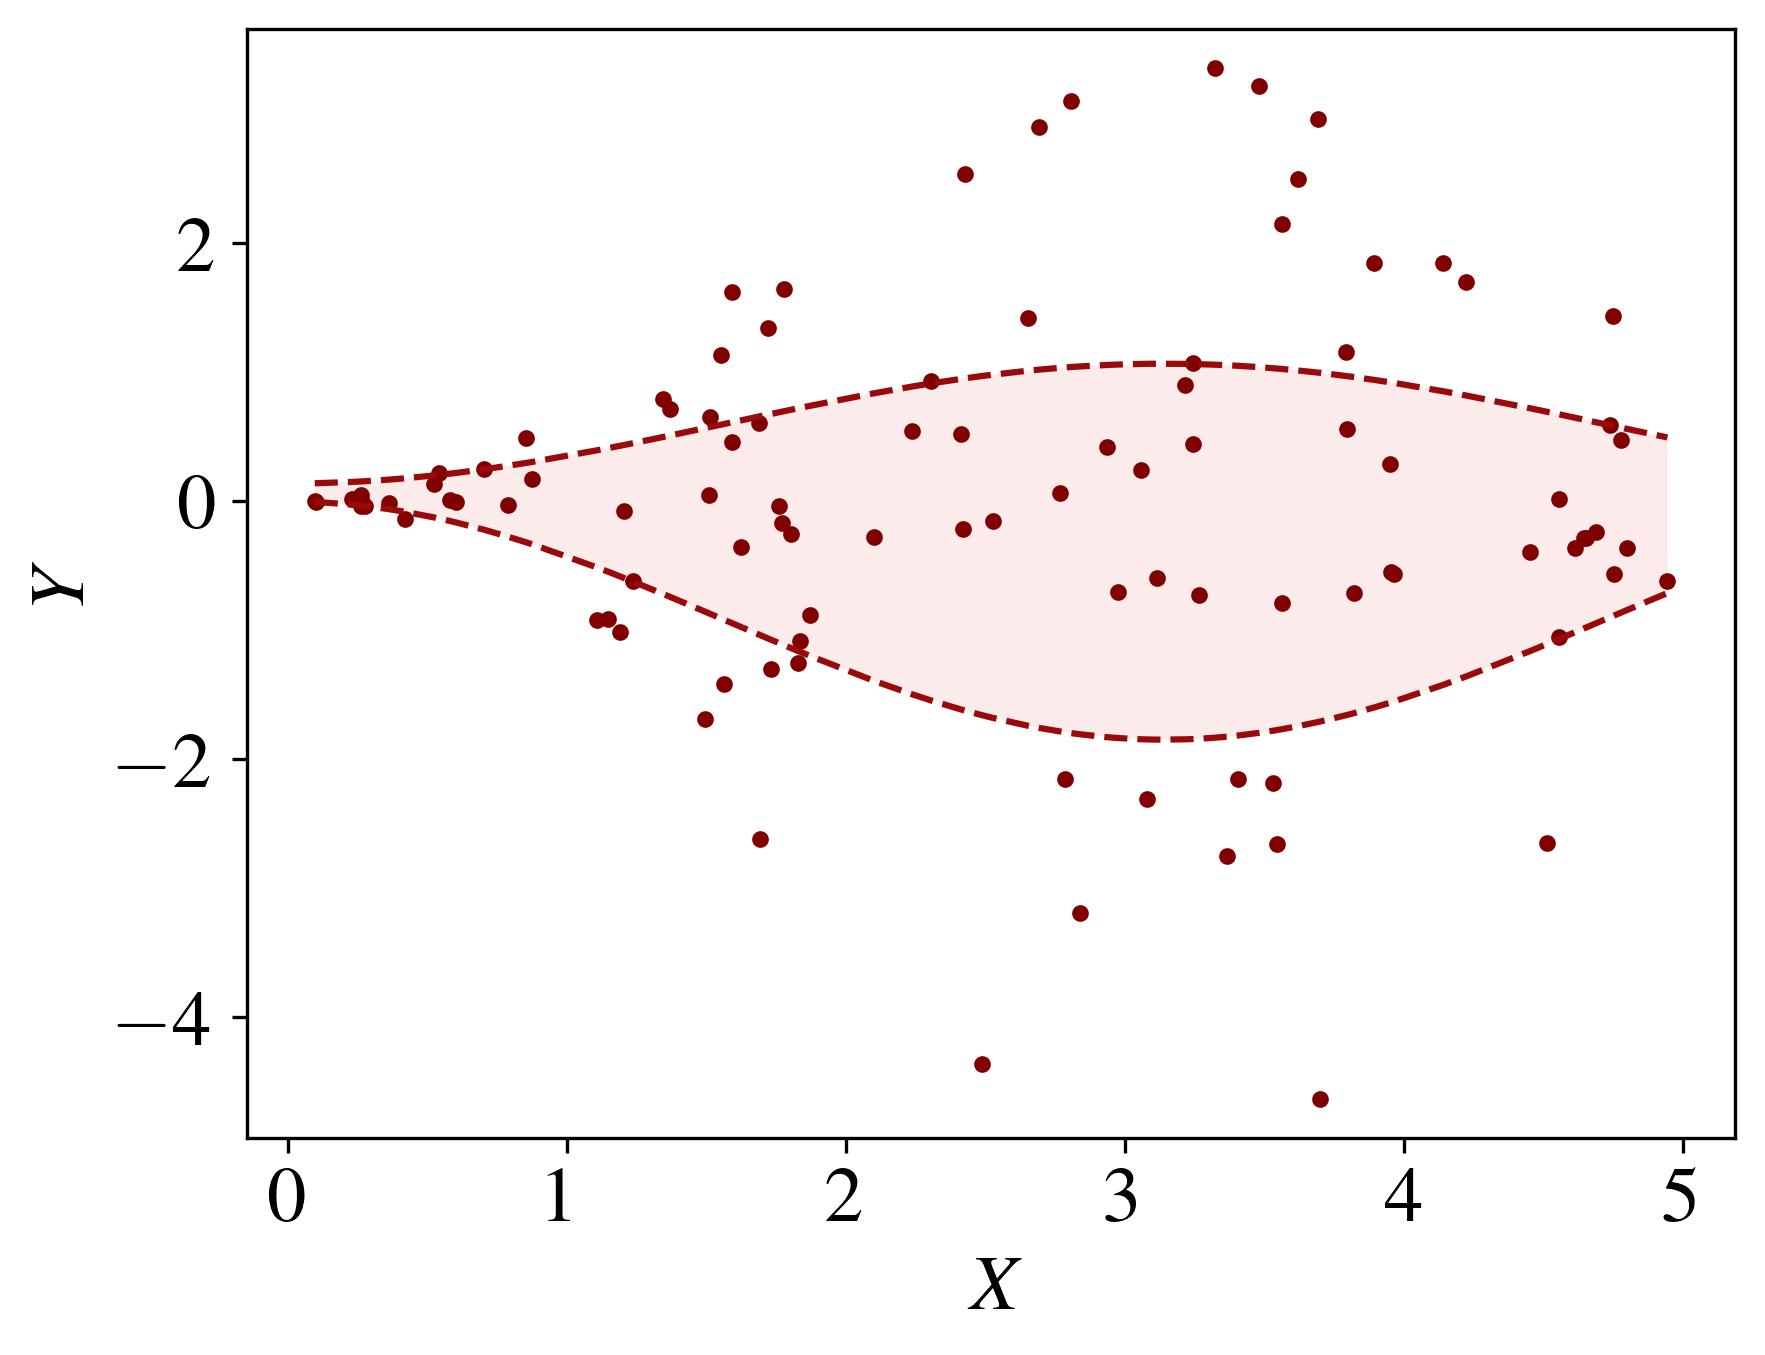
\includegraphics[width=\textwidth]{Figures/coverage/no-coverage.png}
        \caption{No coverage}
        \label{fig:coverage:no-cover}
    \end{subfigure}
    \hfill
    \begin{subfigure}[b]{0.3\textwidth}
        \centering
        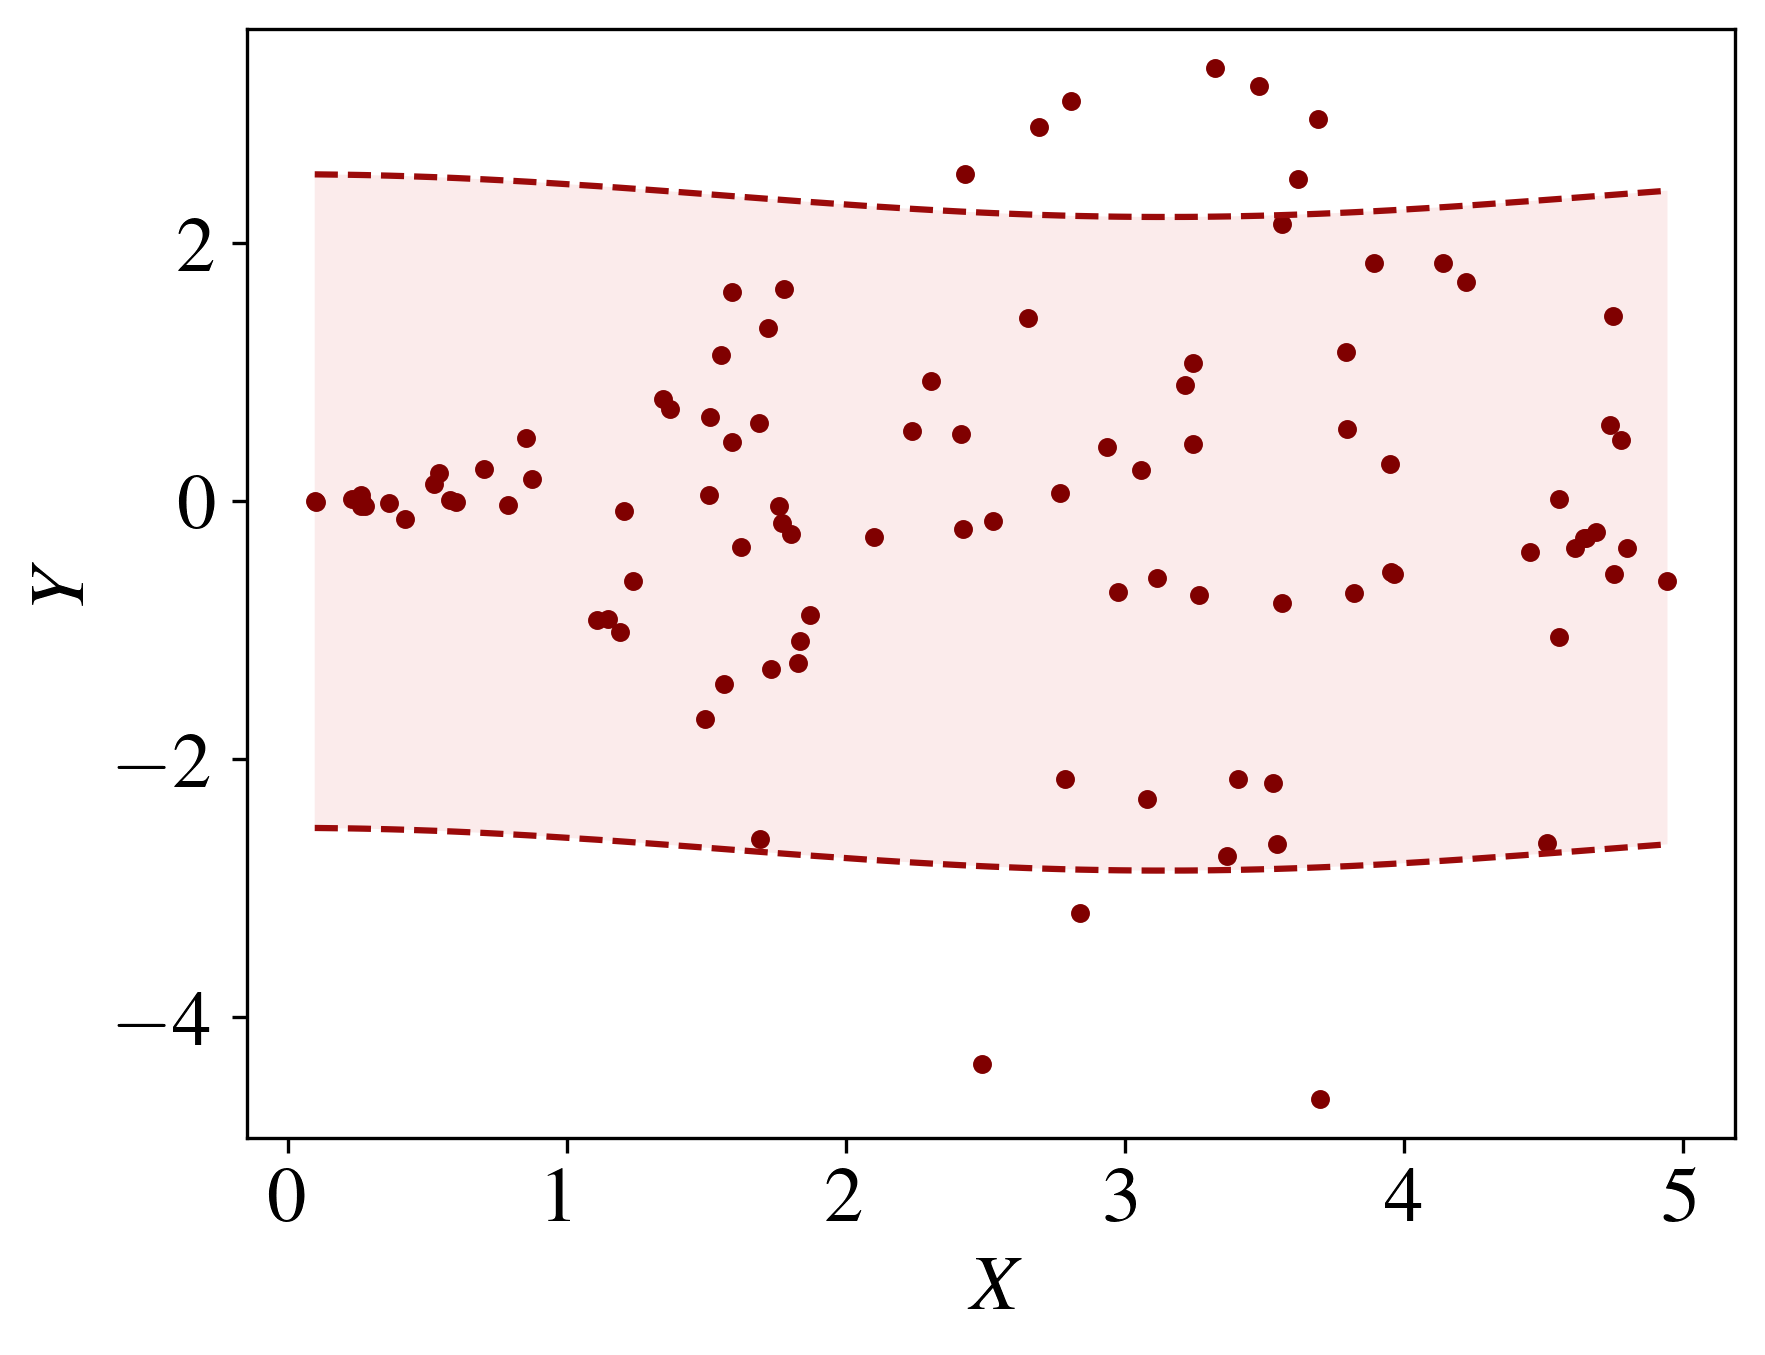
\includegraphics[width=\textwidth]{Figures/coverage/marginal-coverage.png}
        \caption{Marginal coverage}
        \label{fig:coverage:marg-cover}
    \end{subfigure}
    \hfill
    \begin{subfigure}[b]{0.3\textwidth}
        \centering
        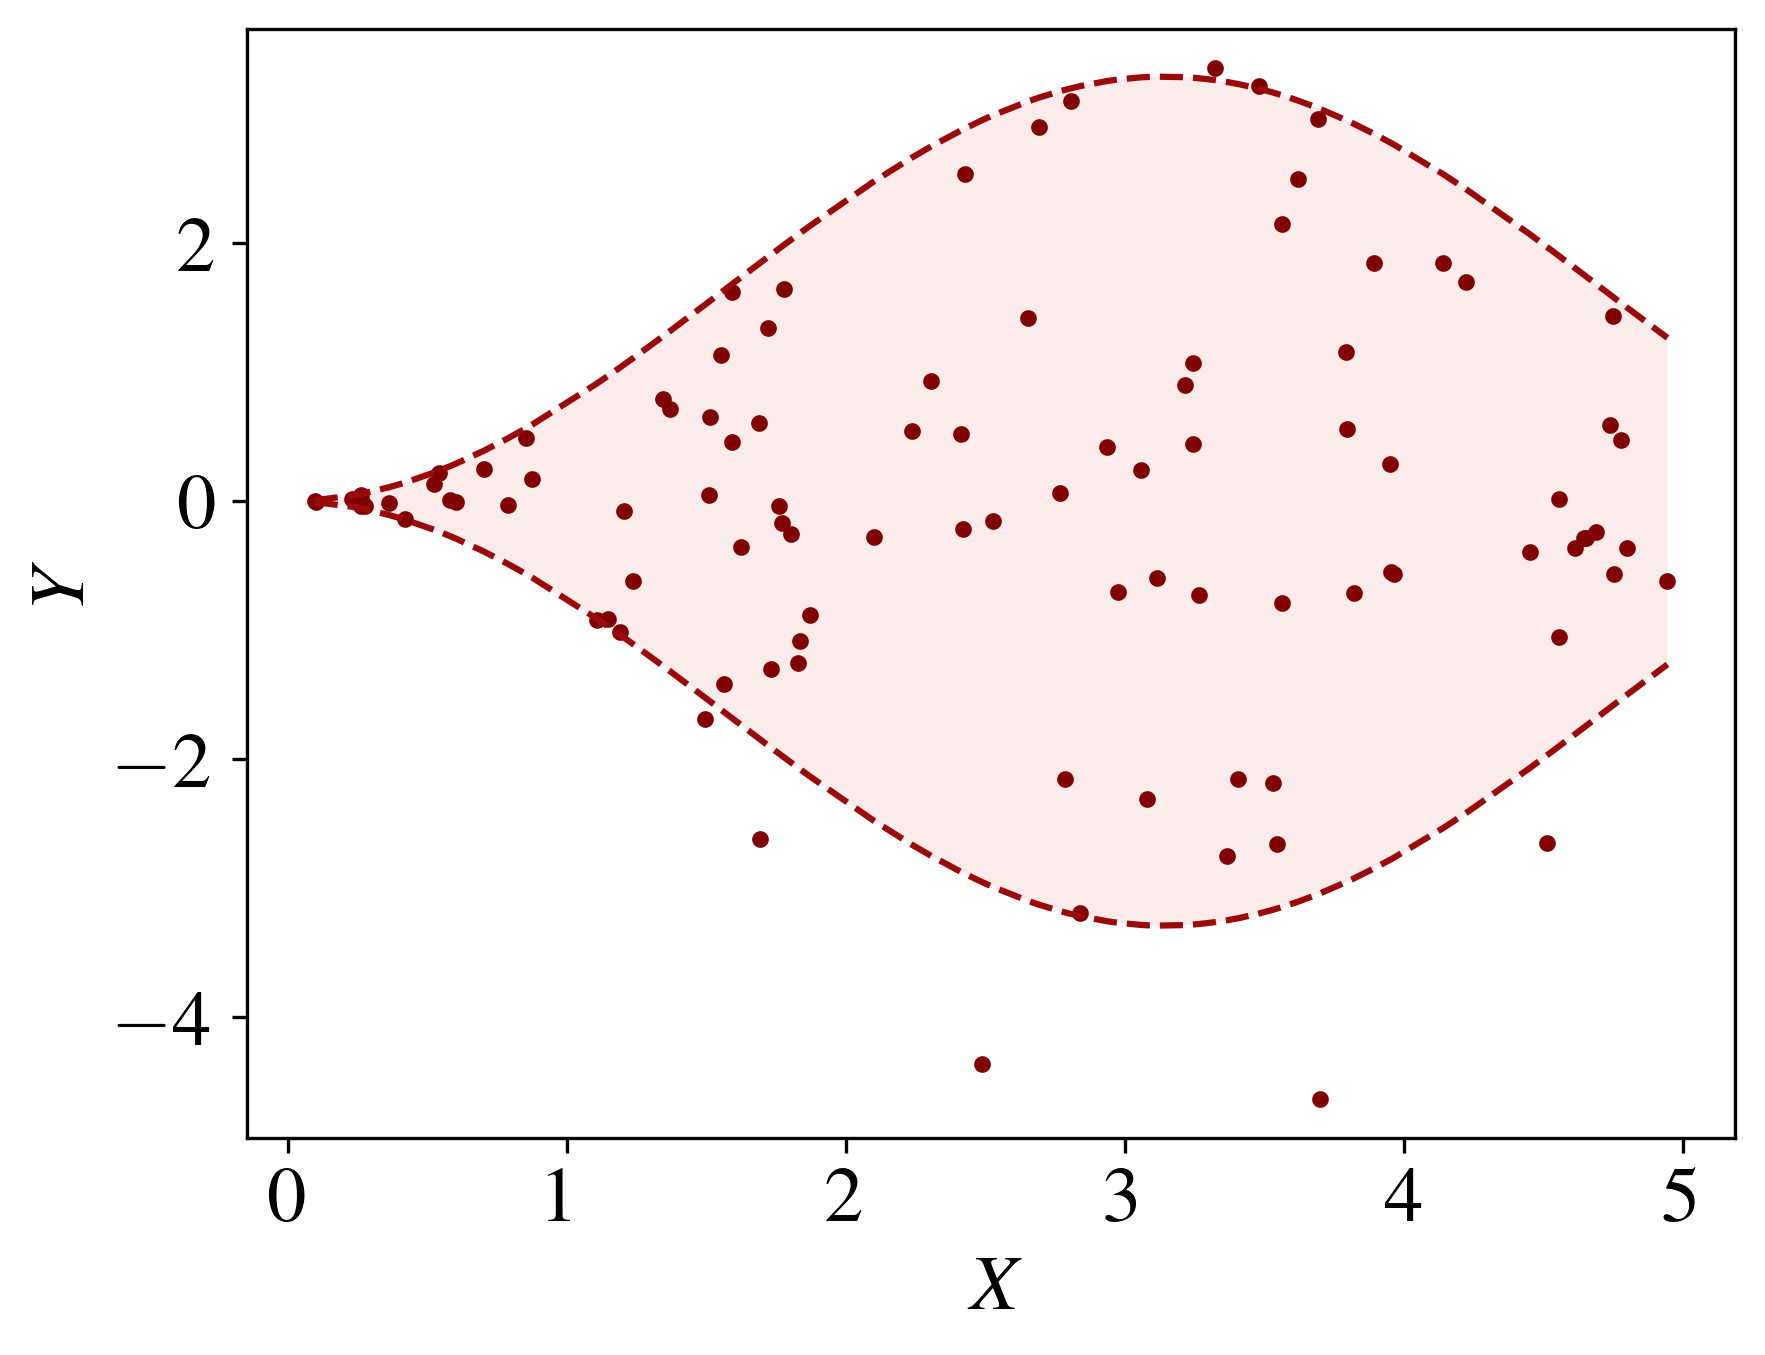
\includegraphics[width=\textwidth]{Figures/coverage/conditional-coverage.png}
        \caption{Conditional coverage}
        \label{fig:coverage:cond-cover}
    \end{subfigure}
    \caption{Different types of coverage. Plots based in \cite{cptuto}.}
    \label{fig:coverage}
\end{figure}

Now, in the general setup, these predictions intervals $\Ca$ should be valid in finite samples and agnostic not only to the data distribution but also to the model used to predict $\Hat{Y}_{n+1}$. 

Within this data-agnostic setup, in section \ref{sec:intro-quantile} quantile regression is reviewed as a historical baseline; then, in section \ref{sec:intro-conformal} conformal prediction will be presented as means of producing $\Ca$ with statistical valid coverage.

\section{Quantile regression}\label{sec:intro-quantile}

Introduced by \cite{koenker}, quantile regression focuses on estimating either boundaries of the distribution (quantiles) for a regression problem. Unlike classical linear regression, which predicts dependent variable's median given independent variables; quantile regression predicts a quantile, providing a more comprehensive analysis of possible outcome distributions.\\

Essentially, given the quantile level $\beta\in\left[0,\ 1\right]$, one can find a estimator for $\beta$ by adapting the loss function using the so-called \textit{pinball loss}:
$$ \ell_\beta\left(Y, Y^{\prime}\right)=\beta\left|Y-Y^{\prime}\right| \mathbb{1}_{\left\{\left|Y-Y^{\prime}\right| \geq 0\right\}}+(1-\beta)\left|Y-Y^{\prime}\right| \mathbb{1}_{\left\{\left|Y-Y^{\prime}\right| \leq 0\right\}} $$

Thence, during the fitting process of a estimator $\mu_\beta$ for the quantile $\beta$ - where $Y\sim \mu\left(X\right)$ -, the following loss function can be defined: $$L_{\mu_\beta}(X, Y):= \mathbb{E}\left[\ell_\beta\left(Y,\Hat{\mu_{\beta}}(X)\right)\right],$$ as the loss function.

As discussed by \cite{cptuto}, if $\Hat{\mu}\in \mathrm{argmin}_{\mu} L_{\mu_\beta}$, then $\Hat{\mu}\equiv Q_{X|Y}(\beta):=\mathrm{inf}\{x\in\R,\mathbb{P}(X\leq x|Y)\geq \beta\}$ is the $\beta$ quantile function.\\

Thus, the naive approach to obtain a predictive interval with $\alpha$ miscoverage level ($1-\a$ confidence) could be to fit the dependent variable's distribution, in terms of the independents $X$, with this adapted loss function and, then, prescribe:
$$ \Ca(X_{n+1}) = \left[ \Hat{\mu}_{\frac{\a}{2}}\left(X_{n+1}\right),\ \Hat{\mu}_{1-\frac{\a}{2}}\left(X_{n+1}\right) \right], $$ for a new sample $X_{n+1}$.

However, since $\mu_{\frac{\a}{2}}$ \& $\mu_{1-\frac{\a}{2}}$ have been trained just with $\{(X_i,Y_i)_{i=1}^n\}$, it could happen $\Ca$ is under/over-confident out of training. Namely, for a finite sample, there is no theoretical guarantee $\Ca$ has statistical valid coverage: $$ \mathbb{P}\left(Y_{n+1} \in \left[ \Hat{\mu}_{\frac{\a}{2}}\left(X_{n+1}\right),\ \Hat{\mu}_{1-\frac{\a}{2}}\left(X_{n+1}\right) \right] \right) \ne 1 - \a $$

In conclusion, though providing an approximate measure of the target's variability, quantile regression (QR) does not inherently constitute a framework for providing statistically valid predictive sets.

\section{Conformal prediction}\label{sec:intro-conformal}

Initially developed in the early 2000s by Vladimir Vovk, Alexander Gammerman, and Glenn Shafer; conformal prediction (CP) was born as a framework for producing statistically valid, data-agnostic \& distribution-free predictive sets. 

Heuristically, CP is based on the idea of using the samples data, not only to train the estimator $\mu$, but also to "conformalize" the model with the data so that the predictive sets attain the expected coverage (unlike in QR \ref{sec:intro-quantile}). 

In this sense, CP is based on the idea of using this "past" (sample) data to determine how the model errors are distributed and, thus, its conformity to the "reality". This is measured in terms of the so-called conformity score.\\ 

Notice, nevertheless, CP requires at least one assumption to ensure its validity. Since the model conformity measure is evaluated on the same samples from which the training set is created, the data needs to be \textbf{exchangeable} (\textit{i.e.} any permutation of samples should not affect the joint distribution). A thorough explanation and theoretical justification of CP, along the different methodologies to implement CP (with options for trading-off computational or statistical efficiency), is presented in chapter \ref{chap:conformal-prediction}.
% Introduction

\chapter{Conformal prediction}

\label{chap:conformal-prediction}

%---------------------------------------
%	SECTION 1: Conformal Prediction (CP)
%---------------------------------------

% \section{Conformal Prediction}\label{sec:cp}

Leveraging same notation as in chapter \ref{chap:intro}, and given $(X, Y)\in \R^d\times\R$ random variables with unknown marginal and joint probability distributions, we want to obtain a $\Ca$ predictive interval. Let us address the case in which $Y=\mu(X) + \epsilon$, where $\mu$ is the model function to be determined and $\epsilon_i\sim P_{Y|X}$ the noise. From now on, we will only assume the data to be \textbf{exchangeable}. 

% For this regression problem we will use the formerly mentioned $n$ samples $(X_i, Y_i)_{i=1}^{n}$, and from now on we will only assume the data to be \textbf{exchangeable}. 

\begin{definition}[Exchangeability]
$\left(X_i, Y_i\right)_{i=1}^n$ are exchangeable if, for any permutation $\sigma$ of $\left[ 1, n \right]$ :
$$
\mathcal{L}\left(\left(X_1, Y_1\right), \ldots,\left(X_n, Y_n\right)\right)=\mathcal{L}\left(\left(X_{\sigma(1)}, Y_{\sigma(1)}\right), \ldots,\left(X_{\sigma(n)}, Y_{\sigma(n)}\right)\right),
$$
where $\mathcal{L}$ designates the joint distribution.
\end{definition}

\begin{example}
    Independent identically distributed (\textit{i.i.d}) samples, or the components of a multidimensional normal distribution, are exchangeable data.
\end{example}
\begin{example}
    Time series data, as well as data obtained from a random variable under any kind of distribution shift, are examples of non-exchangeable data.
\end{example}

Furthermore, as mentioned in section \ref{sec:intro-conformal}, conformal prediction is ultimately based in using the so-called \textit{conformality scores} to construct the predictive interval. These scores, $s_{\Hat{\mu}}$ or directly $s$, allow to transform a heuristic notion of uncertainty from a model $\Hat{\mu}$ into a rigorous measure of it.

Formally, any function $s(X, Y)\in\R$ can be chosen as score if it returns larger values the worse the agreement between $X$ and $Y$ is. Note the choice of conformity score will determine the way confidence intervals are built. 
In particular, the simplest choice is the absolute residual score (namely, the residual) as score for the regression problems: $s_i := s_{\Hat{\mu}}(X_i,Y_i) = \left| Y_i - \Hat{\mu}(X_i) \right|$. 

In this case, then, the predictive intervals is built as 
\begin{equation*}
    \Hat{\Ca} = \left[ 
\Hat{\mu}(X) - q(\mathcal{S}),\ \Hat{\mu}(X) + q(\mathcal{S}) \right],
\end{equation*} where $q(\mathcal{S})$ is the $1-\a$ empirical quantile of the conformity scores $\mathcal{S}=\{s_i\}_{i}$.

\begin{note}
    The \textit{conformity score} election can play a pivotal role in the uncertainty quantification process. In particular, useless or no informative intervals can be obtained in function of the chosen score, as explained in \cite{gentleintro}.
\end{note}

\begin{example}
    There are other well-known scores, for instance those implemented by \cite{mapie:scores}:
    \begin{itemize}
        \item Gamma score $s_{\Hat{\mu}}(X,Y) := \frac{\left| Y - \Hat{\mu}(X) \right|}{\Hat{\mu}(X)}$, such that: \begin{equation*}
            \Hat{\Ca} = \left[ 
\Hat{\mu}(X)\left(1 - q(s)\right),\ \Hat{\mu}(X)\left(1 + q(s)\right) \right]
        \end{equation*}
        \item Residual normalized score $s_{\Hat{\mu}}(X,Y) := \frac{\left| Y - \Hat{\mu}(X) \right|}{\Hat{\sigma}(X)}$, where $\Hat{\sigma}(X)$ is another model which predicts residuals from $X$ (trained on $(X, \left|Y-\Hat{\mu}(X)\right|)$), and it is such that: \begin{equation*}
            \Hat{\Ca} = \left[ 
\Hat{\mu}(X) - q(s)\Hat{\sigma}(X),\ \Hat{\mu}(X) + q(s)\Hat{\sigma}(X)\right]
        \end{equation*}
    \end{itemize}
\end{example}

Within the same conformity score setup, however, several approaches for CP can be applied in function of the user needs regarding computational and statistical efficiency. In this sense, from sections \ref{sec:scp} to \ref{sec:other-flavours}, different CP flavours will be presented; while, in section \ref{sec:cqr}, a way of "\textit{conformalizing}" the quantile regression method is reviewed. Finally, section \ref{sec:guarantees-limits} is devoted the theoretical guarantees and limits of CP and its flavours.

% \subsection{Naive method}

% This approach computes the residuals of the training data to estimate the typical error obtained on a new test data point. Thus, the interval is given by the prediction $\Hat{\mu}(X)$ and adding/subtracting the quantiles of the conformity scores $q(s)$ of the \textbf{same training set}:

% \begin{equation*}
%     \Hat{\Ca}^{\mathrm{naive}}_{n, \a}(X_{n+1}) = \Hat{\mu}(X_{n+1}) \pm \Hat{q}^{+}_{n,\a}(\left|Y_i - \Hat{\mu}(X_i)\right|) =: \Hat{\mu}(X_{n+1}) \pm \Hat{q}^{+}_{n,\a}(s_i), 
% \end{equation*} if we set $s_i:=\left|Y_i - \Hat{\mu}(X_i)\right|$ from now on.

% Of course, however, this method does not attain valid statistical coverage and underestimates the width of prediction intervals because of a potential overfit (the conformity scores are estimate only on the training set).

\section{Split Conformal Prediction}\label{sec:scp}

Split Conformal Prediction (SCP) is the most widely-used flavour of conformal prediction and it is based in splitting the data in a training $\mathrm{Tr}$ set and a calibration $\mathrm{Cal}$ set. Thus, if we used the absolute residual as conformity score, SCP would prescribe as it follows:

\begin{enumerate}
    \item Split the data set into a \textbf{training set} of size $\#\mathrm{Tr}$ and a \textbf{calibration set} of size $\#\mathrm{Cal}$
    \item Obtain $\Hat{\mu}$ by training the algorithm in the $\mathrm{Tr}$ set
    \item Obtain a set $\S$ of conformity scores by using the $\mathrm{Cal}$ set: $\S_{\mathrm{Cal}}:=\{ s_i \}_{i\in \mathrm{Cal}}=\{ \left|Y_i - \Hat{\mu}(X_i)\right|, i\in \mathrm{Cal}\}$
    \item Compute $q_{1-\a^{\mathrm{SCP}}}(\S_{\mathrm{Cal}})$, namely the $(1-\a)\left(\frac{1}{\#\mathrm{Cal}}+1\right)$ quantile of $\S_{\mathrm{Cal}}$. From now on, we will indistinctly write $q_{1-\a^{\mathrm{SCP}}}(\S_{\mathrm{Cal}})\equiv q_{1-\a}(\S_{\mathrm{Cal}})$
    \item For a new sample $X_{n+1}$, return the predictive interval
    \begin{equation}
        \label{eq:scp}
        \Hat{\Ca} = \left[\Hat{\mu}(X_{n+1}) - q_{1-\a}(\S_{\mathrm{Cal}}),\ \Hat{\mu}(X_{n+1}) + q_{1-\a}(\S_{\mathrm{Cal}})\right]
    \end{equation}
\end{enumerate}

\begin{note}
    To attain at least $1 - \a$ coverage taking into account the finite number of samples in the $\mathrm{Cal}$ set, in step 4 the quantile of conformity scores $q_{1-\a^{\mathrm{SCP}}}(\S)\equiv q_{1-\a}(\S)$ must be computed as a $(1-\a)\left(\frac{1}{\#\mathrm{Cal}}+1\right)$-quantile (instead of a $(1-\a)$-quantile), the so-called \textbf{$1-\a$ empirical quantile}.
\end{note}

Let us, in Algorithm \ref{alg:SCP}, state the algorithm independently of the conformity score $s$ choice.

\begin{algorithm}
\caption{SCP algorithm}\label{alg:SCP}
\begin{algorithmic}[1] 
\REQUIRE Regression algorithm $\A$, miscoverage level $\a$, data samples $\{\left(X_t,Y_t\right)\}^T_{t=1}$. 
\ENSURE Prediction interval $\Ca(X) \text { for any } X \in \R^d$. 
\STATE Randomly split $\{1, \ldots, T\}$ into two disjoint sets $\mathrm{Tr}$ and $\mathrm{Cal}$. 
\STATE Fit a mean regression function: $\hat{\mu}(\cdot) \leftarrow \mathcal{A}\left(\left\{\left(X_t,Y_t\right), t \in \mathrm{Tr}\right\}\right)$. 
\FOR {$j \in \mathrm{Cal} $} 
\STATE Set $s_j$ the \textit{conformity scores}. 

\hspace{4mm} Note if we chose \textit{e.g.} the absolute residual as conformity score, then $s_j := s_{\Hat{\mu}}(X_j, Y_j) = |Y_j-\hat{\mu}(X_j)|$.

\ENDFOR
\STATE Set $\S_{\mathrm{Cal}} = \{s_j, j\in \mathrm{Cal}\}$.
\STATE Compute $q_{1-\a}\left(\S_{\mathrm{Cal}}\right)$, the $(1-\a )\left(1+1/\left|\mathrm{Cal}\right|\right)$ quantile of $\S_{\mathrm{Cal}}$ (\textit{i.e.} the $1-\a$ empirical quantile).
\STATE Return $\Ca(X) = \{Y \in \R\ |\ s_{\Hat{\mu}}(X, Y) \leq q_{1-\a}(\S_{\mathrm{Cal}}) \}$, for any $X \in \R^d$. 

\hspace{4mm} Note the explicit form of $\Ca(x)$ depends on the conformality score; \textit{e.g.} if we chose the absolute residual, then $\Ca(X) = \left[\hat{\mu}(X)\pm q_{1-\a}\left(\S_{\mathrm{Cal}}\right)\right]$.

\end{algorithmic}
\end{algorithm}

Notice SCP requires that one must have enough observations to split its original dataset into train and calibration, but at least it attains the expected coverage of $\geq 1 -\a$. This will be theoretically backed later at section \ref{guarantees:scp}, particularly through Theorem \ref{thm:scp}.

\section{Full Conformal Prediction}\label{sec:fcp}

Even though SCP attains expected coverage and just needs to fit a model $\mu$ once (thus, it is not computationally demanding), the dataset needs to be large enough for $\Ca$ to be informative. 

Full Conformal Prediction (FCP) is born as a workaround to this problem. Unlike SCP, FCP leverages the whole dataset as training and its core idea is as stated at \cite{gentleintro}.\\

Let us assume the dataset $\{(X_t, Y_t)\}_{t=1}^{T}$ is available and, for a new sample $X_{T+1}$, the user wants to provide the interval $\Ca(X_{T+1})$. Then, since the true label $Y_{T+1}$ lies somewhere in $\mathcal{Y} := \mathrm{Im}(\mu)\subset\R$, looping over all possible $Y\in\mathcal{Y}$ will eventually hit in the $(X_{T+1}, Y_{T+1})$ data point which is exchangeable with the first $T$ points; specifically, the most probable labels will have a low enough conformity score.\\

FCP, as explained in Algorithm \ref{alg:FCP}, consists in: "\textit{discretizing}" the target space $\mathcal{Y}$ into $N$ candidates $Y_j$, traversing this loop fitting the estimator to the data \& $(X_{T+1},Y_{j})$ as new data point, and finally returning those candidates $Y_{j}$ such that they "conform enough" to the data. The latter condition will be translated to asserting whether the conformity score of $Y_{j}$ candidate is "low enough" (lower than the $1-\alpha$ empirical quantile of all conformity scores $\mathcal{S}$).\\

\begin{algorithm}
\caption{FCP algorithm}\label{alg:FCP}
\begin{algorithmic}[1] 
\REQUIRE Regression algorithm $\A$, miscoverage level $\a$, data samples $\{\left(X_t,Y_t\right)\}^T_{t=1}$ and new $X_{T+1}$ feature sample. 
\ENSURE Prediction interval $\Ca(X_{T+1}) \text { for any given } X_{T+1} \in \R^d$. 
\STATE Discretize the target space $\mathcal{Y}$ reducing into $N$ candidates $Y_j$. 
\STATE Initialize $\Hat{\mathcal{Y}}_{\mathrm{low}} = \{\}$ the array for candidates with "low enough" conformity score
\FOR {$j \in \{1, \ldots, N\},\ Y_j$ candidate} 
\STATE Fit a mean regression function $\mu_j$ using $\mathrm{Tr}_j=\{\left(X_t,Y_t\right)\}^T_{t=1}\cup \{(X_{T+1}, Y_j)\}$ as training data: $$\hat{\mu}_j(\cdot) \leftarrow \mathcal{A}\left(\left\{\left(X_t,Y_t\right), t \in \mathrm{Tr}_j\right\}\right)\ .$$
\STATE Set $\S_j=\{ s_{\Hat{\mu}_j}(X_i, Y_i) \}_{i=1}^T\cup \{s_{\Hat{\mu}_j}(X_{T+1}, Y_j)\}$ the conformity scores obtained in the same $\mathrm{Tr}_j$ training data.
\STATE Set $q^j_{1 - \a}(\S_{j})$ the $(1-\a )\left(1+\frac{1}{T+1}\right)$ quantile of $\S_{j}$ (\textit{i.e.} the $1-\a$ empirical quantile)
\IF {$s_{\Hat{\mu}_j}(X_{T+1}, Y_j) \leq q^j_{1 - \a}(\S_{j})$}
\STATE Add $Y_j$ to $\Hat{\mathcal{Y}}_{\mathrm{low}}$
\ENDIF

\ENDFOR
\STATE Return $\Ca(X_{T+1}) = \Hat{\mathcal{Y}}_{\mathrm{low}}$.

\end{algorithmic}
\end{algorithm}

Note FCP solves the problem of effectively reducing the dataset through a split, at expenses of a huge computational efforts. In particular, FCP requires to re-fit the model $N$ times for every new $X_{T+1}$ feature sample.

Of course, the existence of $N$ is due to the fact we need to discretize $\mathcal{Y}$ to compute $\Ca(X_{T+1})$. In this sense, the larger $N$ the more accurate FCP will be, but then the more time it will take to infer the predictive set. 

Notice that in the non-discrete case (\textit{i.e.} when $N\rightarrow+\infty$) we would be returning the continuous set $$\Ca(X_{T+1}) = \{Y \in\R\ |\ s_{\Hat{\mu}_j}(X_{T+1}, Y) \leq q^j_{1 - \a}(\S_{j}) \}\ .$$

\section{Other flavours}\label{sec:other-flavours}

On the one hand, in \ref{sec:scp} it is shown split conformal prediction requires only one model fitting step, but sacrifices statistical efficiency. On the other hand, in \ref{sec:fcp} is reviewed how full conformal prediction requires a very large number of model fitting steps, but has high statistical efficiency. These are not the only two achievable points on the spectrum: but there are techniques that precisely fall in between, trading off statistical efficiency and computational efficiency differently.

As represented in Figure \ref{fig:trade-off}, this is the case of cross-conformal prediction CV+ (\cite{vovk2015}) and Jackknife+ (\cite{barber2021b}), methods which both use a small number of model fits, but still leveraging all data for both model fitting and calibration.\\

\begin{figure}%[h]
    \centering
    % \includegraphics{}
    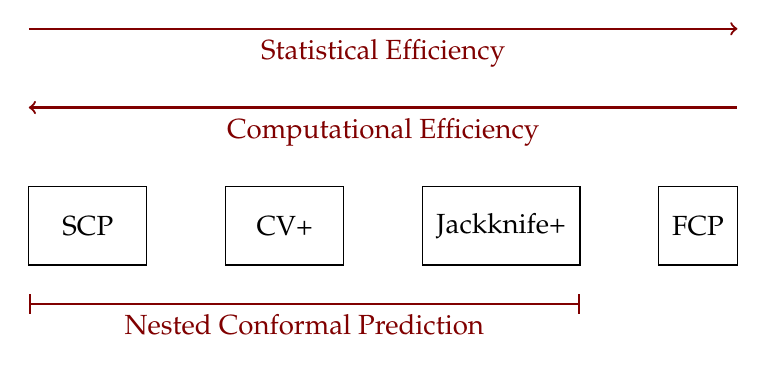
\begin{tikzpicture}
        \definecolor{tred}{HTML}{800000}
        % Draw the horizontal arrows
        \draw[thick, ->, tred] (1, 0) -- (10, 0) node[anchor=north, pos=0.5] {Statistical Efficiency};
        \draw[thick, <-, tred] (1, -1) -- (10, -1) node[anchor=north, pos=0.5] {Computational Efficiency};
        % Draw the boxes
        \draw (1, -3) rectangle (2.5, -2) node[pos=0.5] {SCP};
        \draw (3.5, -3) rectangle (5, -2) node[pos=0.5] {CV+};
        \draw (6, -3) rectangle (8, -2) node[pos=0.5] {Jackknife+};
        \draw (9, -3) rectangle (10, -2) node[pos=0.5] {FCP};
        % Draw the nested conformal prediction arrow
        \draw[thick, |-|, tred] (1, -3.5) -- (8, -3.5) node[anchor=north, pos=0.5] {Nested Conformal Prediction};
    \end{tikzpicture}

    \caption{Representation of the trade-off between statistical and computational efficiencies for the different approaches. Based on \cite{cptuto}.}
    \label{fig:trade-off}
\end{figure}

On the one hand, the so-called Jackknife+ method is based on leave-one-out (LOO) and, for a new $X_{n+1}$, it heuristically prescribes:
\begin{enumerate}
    \item For each $i\in\mathcal{D}:=\{1,\ldots, T\}$ sample of the training data:
    \begin{itemize}
        \item Fit a mean regression function $\mu_{-i}$ training $\mathcal{A}$ in $\mathcal{D}\setminus (X_i, Y_i)$: $$\hat{\mu}_{-i}(\cdot) \leftarrow \mathcal{A}\left(\left\{\left(X_t,Y_t\right), t \in \mathcal{D}\setminus (X_i, Y_i)\right\}\right)\ .$$
        \item Get the conformity scores $$\S^i_{\mathrm{up/down}} = \hat{\mu}_{-i}(X_{n+1}) \pm s_{\hat{\mu}_{-i}}(X_i, Y_i) $$
    \end{itemize}
    \item Set the conformity scores' sets: $\S_{\mathrm{up}} = \{\S^i_{\mathrm{up}}\}_{i\in\mathcal{D}}$ and $\S_{\mathrm{down}} = \{\S^i_{\mathrm{down}}\}_{i\in\mathcal{D}}$
    \item Defining $q_{\beta,\mathrm{inf}}(Z_1, \ldots,Z_n)$ as the $\lfloor\beta\times n\rfloor$ smallest value of $(Z_1, \ldots,Z_n)$, and $q_{1-\a}$ the $1-\a$ empirical quantile; the following predictive interval is returned: $$ \Hat{\Ca}(X_{n+1}) = \left[q_{\a,\mathrm{inf}}(\S_{\mathrm{down}}),\ q_{1-\a}(\S_{\mathrm{up}})\right] $$
\end{enumerate}

Note, however, J$+$aB may be more computationally demanding even than FCP if the dataset is large such $T>N$ (more samples $T$ than $N$ points needed to \textit{discretize} the $\mathcal{Y}$ space in FCP). 

On the other hand, the CV+ method is based on cross-validation residuals and precisely extends the previous idea into a "batch" of samples. Thence, the following differences must be taken into account:
\begin{itemize}
    \item Instead of leaving one out of $\mathcal{D}$,  CV+ splits the data into $K$ folds $F_1,\ldots, F_K$.
    \item Then, for each $k\in\{1,\ldots, K\}$ fold:
    \begin{itemize}
        \item A mean regression function $\mu_{-{F_K}}$ is fit training $\mathcal{A}$ in $\mathcal{D}\setminus F_k$, instead of $\mathcal{D}\setminus (X_i, Y_i)$.
        \item The conformity scores are no longer a value (for each $i\in\{1,\ldots,N\}$) but a subset (obtained with samples within each fold $k$): $$\S^k_{\mathrm{up/down}} = \{\hat{\mu}_{-k}(X_{n+1}) \pm s_{\hat{\mu}_{-k}}(X_i, Y_i)\}_{i\in F_k} $$
    \end{itemize}
\end{itemize}

Notice this method enhances the computational efficiency at expenses of the statistical's, by training $\A$ less times (and with less data). For a precise and complete description of the algorithms, we refer the reader to the former works (\cite{vovk2015} and \cite{barber2021b}).

%---------------------------------------
%	SECTION 1: Conformalized QR (CQR)
%---------------------------------------

\section{Conformalized Quantile Regression}\label{sec:cqr}

While the former flavours of conformal prediction have theoretical guarantees for its statistical coverage, just marginal coverage is sought thus providing non-adaptive predictive intervals: $$ \mathbb{P}\left\{Y_{n+1} \in \Hat{\Ca}\left(X_{n+1}\right) \cancel{ \mid X_{n+1}=x }\right\} \geq 1-\a $$

In this section, thence, we present the Conformalized Quantile Regression (CQR) as means of obtaining more adaptive intervals $\Ca$. As discussed in \ref{guarantees:limits}, notice that while approximate and asymptotic conditional coverage can be sought, conformal prediction (even within CQR) does not guarantee it without further assumptions than data exchangeability. Nevertheless, at practice, CQR will allow us to obtain more informative intervals.\\

CQR proposes to fit not one $\mu$ but two models $\mu_{\mathrm{down}}$ and $\mu_{\mathrm{up}}$ and adjusting the conformality score $s_{\mu}$ to: \begin{equation}\label{eq:cqr-score}
    s_{\A}(X_i,Y_i):=\mathrm{max}\left( {\hat{\mu}}_{\mathrm{down}}(X_i) - Y_i,\ Y_i - {\hat{\mu}}_{\mathrm{up}}(X_i)\right)
\end{equation}

The model $\mu_{\mathrm{down}}$ and $\mu_{\mathrm{up}}$ are no longer trying to capture the mean value of $(X,Y)$, but rather the low and high quantiles of their distribution (\textit{e.g.} $\mu_{\mathrm{down}}$ \& $\mu_{\mathrm{up}}$ could be estimators of the $\a/2$ and $1-\a/2$ quantiles). In this sense, CQR achieve adaptive predictive intervals by adding/subtracting the conformity score to the inferred values of 2 different estimators.

Thus, CQR is not a different methodology but another "choice" of conformity score definition and it is compatible with the SCP or FCP approaches (or others such as Jackknife+, CV+...). 

Let us see, as an example in Algorithm \ref{alg:CQR}, what CQR prescribes if we use the SCP approach:

\begin{algorithm}
\caption{CQR algorithm (using split prediction)}\label{alg:CQR}
\begin{algorithmic}[1] 
\REQUIRE Regression algorithm $\A$, miscoverage level $\a$, data samples $\{\left(X_t,Y_t\right)\}^T_{t=1}$. 
\ENSURE Prediction interval $\Ca(X) \text { for any } X \in \R^d$. 
\STATE Randomly split $\{1, \ldots, T\}$ into two disjoint sets $\mathrm{Tr}$ and $\mathrm{Cal}$. 
\STATE Fit 2 regression functions, one for the lower quantile $\hat{\mu}_{\mathrm{down}}$ and one for the upper $\hat{\mu}_{\mathrm{up}}$: $$\hat{\mu}_{\mathrm{down}}(\cdot), \hat{\mu}_{\mathrm{up}}(\cdot) \leftarrow \mathcal{A}\left(\left\{\left(X_t,Y_t\right), t \in \mathrm{Tr}\right\}\right)\ .$$ 
\vspace{-4mm}

\FOR {$j \in \mathrm{Cal} $} 
\STATE Set $s_j$ the \textit{conformity score} using \ref{eq:cqr-score}: $$s_j := s_{\A}(X_j, Y_j)=\mathrm{max}\left(\hat{\mu}_{\mathrm{down}}(X_i) - Y_i,\ Y_i - \hat{\mu}_{\mathrm{up}}(X_i)\right)$$ 
\vspace{-5mm}
\ENDFOR
\STATE Set $\S_{\mathrm{Cal}} = \{s_j, j\in \mathrm{Cal}\}$.
\STATE Compute $q_{1-\a}\left(\S_{\mathrm{Cal}}\right)$, the $(1-\a )\left(1+1/\left|\mathrm{Cal}\right|\right)$ quantile of $\S_{\mathrm{Cal}}$ (\textit{i.e.} the $1-\a$ empirical quantile).
\STATE Return $\Ca(X_{n+1}) = \left[\hat{\mu}_{\mathrm{down}}(X_{n+1}) - q_{1-\a}\left(\S_{\mathrm{Cal}}\right),\ \hat{\mu}_{\mathrm{up}}(X_{n+1}) + q_{1-\a}\left(\S_{\mathrm{Cal}}\right)\right]$ for any new $X_{n+1} \in \R^d$. 
\end{algorithmic}
\end{algorithm}

%%%%%%%%%%%%%%%%%%%%%%%%%%%%%%%%%%%%%%%%%%%%%%%%%%%%%%%%%%%%%%%

\section{Theoretical guarantees and limits}\label{sec:guarantees-limits}

Even though the heuristic notion justifying the validity of the different paradigms of conformal prediction may be clear, we have not discussed its theoretical guarantees and limits yet. Yet, this is precisely the objective in this section: while in \ref{guarantees:scp} and \ref{guarantees:fcp} we will proof $1-\a$ coverage can be sought in SCP and FCP respectively, in \ref{guarantees:others} we will discuss which are the guarantees for Jackknife+ and CV+, and we will conclude by reviewing the known limits of conformal prediction in \ref{guarantees:limits}.

\subsection{Split Conformal Prediction}\label{guarantees:scp}

Henceforth, in Theorem \ref{thm:scp} and through Lemma \ref{lemma:quantile}, the theoretical guarantee of SCP (algorithm \ref{alg:SCP}) is proven. We reproduce the proof found at \cite{cptuto}, which is general for any conformity score $s$ choice; however, note that:
\begin{itemize}
    \item The proof for the lower bound initially appeared at \cite{papadopoulos} for \textit{i.i.d.} data. Then, \cite{vovk2005} proved that the theorem also holds if the observations satisfy the weaker condition of exchangeability.
    \item The upper bound case was initially proved with Theorem 2.2 of \cite{lei2018} (along the lower bound case, see A.1) but specifically for the absolute residual score case. The proof required the residuals to have a continuous joint distribution, but as mentioned in \cite{gentleintro} this condition is not important because the user can always add a vanishing amount of random noise to the score. 
    \item Both lower and upper bound cases were later stated for the CQR case in Theorem 1 of \cite{romano2019} (and proved in its supplementary material).
\end{itemize}

\begin{lemma}[Quantile lemma]\label{lemma:quantile}
    If $\left(U_1, \ldots, U_n, U_{n+1}\right)$ are exchangeable, then for any $\left.\beta \in\right] 0,1[$: $$ \mathbb{P}\left(U_{n+1} \leq q_\beta\left(U_1, \ldots, U_n,+\infty\right)\right) \geq \beta . $$
    Additionally, if $U_1, \ldots, U_n, U_{n+1}$ are almost surely distinct, then:
$$ \mathbb{P}\left(U_{n+1} \leq q_\beta\left(U_1, \ldots, U_n,+\infty\right)\right) \leq \beta+\frac{1}{n+1} $$
\end{lemma}
\begin{proof}
    First note that $U_{n+1} \leq q_\beta\left(U_1, \ldots, U_n,+\infty\right) \Longleftrightarrow U_{n+1} \leq q_\beta\left(U_1, \ldots, U_n, U_{n+1}\right)$.
Then, by definition of $q_\beta$ :
$$
U_{n+1} \leq q_\beta\left(U_1, \ldots, U_n, U_{n+1}\right) \Longleftrightarrow \operatorname{rank}\left(U_{n+1}\right) \leq\lceil\beta(n+1)\rceil
$$

By exchangeability, $\operatorname{rank}\left(U_{n+1}\right) \sim \mathcal{U}\{1, \ldots, n+1\}$. Thus:
$$
\mathbb{P}\left(\operatorname{rank}\left(U_{n+1}\right) \leq\lceil\beta(n+1)\rceil\right) \geq \frac{\lceil\beta(n+1)\rceil}{n+1} \geq \beta .
$$

If $U_1, \ldots, U_n, U_{n+1}$ are almost surely distinct (without ties):
$$
\begin{aligned}
\mathbb{P}\left(\operatorname{rank}\left(U_{n+1}\right) \leq\lceil\beta(n+1)\rceil\right) & =\frac{\lceil\beta(n+1)\rceil}{n+1} \\
& \leq \frac{1+\beta(n+1)}{n+1}=\beta+\frac{1}{n+1} . \end{aligned}
$$
\end{proof}

% proof for SCP's guarantees
\begin{theorem}[SCP guarantees]\label{thm:scp}
    Suppose $\left(X_i, Y_i\right)_{i=1}^{n+1}$ are exchangeable. SCP applied on $\left(X_i, Y_i\right)_{i=1}^n$ yields $\Hat{\Ca}(\cdot)$ such that:
$$ \mathbb{P}\left\{Y_{n+1} \in \Hat{\Ca}\left(X_{n+1}\right)\right\} \geq 1-\a . $$

Additionally, if the scores $\left\{S_i\right\}_{i \in \mathrm{Cal}} \cup\left\{S_{n+1}\right\}$ are a.s. distinct: $$
\mathbb{P}\left\{Y_{n+1} \in \Hat{\Ca}\left(X_{n+1}\right)\right\} \leq 1-\a+\frac{1}{\# \mathrm{Cal}+1}
$$
\end{theorem}
\begin{proof}
    When $\left(X_i, Y_i\right)^{n+1}_{i=1}$ are exchangeable, the scores $\{S_i\}_{i\in\mathrm{Cal}}\cup \{S_{n+1}\}$ are also exchangeable. Applying Lemma \ref{lemma:quantile} to the scores concludes the proof.
\end{proof}

\subsection{Full Conformal Prediction}\label{guarantees:fcp}

Even though it leverages all data samples, FCP also attains the expected $1-\a$ statistical coverage and the idea in which the proof relies is really similar to the SCP proof (in particular, it strongly relies on the exchangeability of the $s_{n+1}$ conformity score \textit{w.r.t.} $s_{1},\ldots,s_{n}$). 

However, an additional hypothesis is needed and, although related to exchangeability, consists in the algorithm $\A$ being \textit{symmetrical}.  

\begin{definition}[Symmetrical algorithm]
A deterministic algorithm $\A: \left(U_1, \ldots, U_n\right)\rightarrow\hat{A}$ is symmetric if, for any permutation $\sigma$ of $\left[ 1, n \right]$ :
$$ \mathcal{A}\left(U_1, \ldots, U_n\right)\myeq 
 \mathcal{A}\left(U_{\sigma(1)}, \ldots,U_{\sigma(n)}\right)\ .$$
\end{definition}

With this new restraint, the following theorem can now be announced:

% proof for FCP's guarantees
\begin{theorem}[FCP guarantees]\label{thm:fcp}
    Suppose $\left(X_i, Y_i\right)_{i=1}^{n+1}$ are exchangeable and $\A$ is symmetric. FCP applied on $\left(X_i, Y_i\right)_{i=1}^n\cup \{X_{n+1}\}$ yields $\Hat{\Ca}(\cdot)$ such that:
$$ \mathbb{P}\left\{Y_{n+1} \in \Hat{\Ca}\left(X_{n+1}\right)\right\} \geq 1-\a . $$

Additionally, if the scores are a.s. distinct: $$
\mathbb{P}\left\{Y_{n+1} \in \Hat{\Ca}\left(X_{n+1}\right)\right\} \leq 1-\a+\frac{1}{n+1}
$$
\end{theorem}

For sake of length and in view of the similarity of FCP proof \textit{w.r.t.} to SCP's, Theorem \ref{thm:fcp} proof will be skipped. Nevertheless, for a detailed version, the reader can refer to \cite{vovk2005} or \cite{lei2018} (A.1 appendix proof of Theorem 2.1). % see https://arxiv.org/pdf/1604.04173.pdf

% \textcolor{red}{En el teorema de la secció 6.1 de \url{https://arxiv.org/pdf/2107.07511.pdf} citen Vovk 2005.}

\subsection{Other flavours}\label{guarantees:others}

Whereas SCP sacrificed statistical efficiency at expenses of computational efforts by splitting the available dataset in two, FCP proposed the contrary leveraging all the data but at the price of much more model fits; and, so far, we have seen these both two opposite methodologies guarantee $1-\a$ statistical coverage.

In this section, we briefly discuss the state of 2 approaches in-between the spectrum: the Jackknife+ \& the CV+.\\

In this sense, in general, it is seen the Jackknife+ method does not guarantee $1-\a$ statistical coverage. Nevertheless, as proved in \cite{barber2021b}, if $\{(X_i, Y_i)\}_{i=1}^{n+1}$ are exchangeable and $\mathcal{A}$ symmetric, then: $$ \mathbb{P}\left(Y_{n+1}\in \Hat{\Ca}(X_{n+1})\right) \geq 1 - 2\a$$

Yet, \cite{barber2021b} proposes the so-called "\textit{jackknife-minmax}" method to attain $1-\a$ coverage within the jackknife setting; in practice, it is seen the yielded prediction intervals are too conservative.\\

We can refer to the same former reference to find out the CV+ method, proposed in \cite{vovk2015}, is another case in which $1-\a$ coverage is no attained without further assumptions.

Actually, within the same hypothesis of $\{(X_i, Y_i)\}_{i=1}^{n+1}$ being exchangeable and $\mathcal{A}$ symmetric, one can prove that, for CV+:
 $$ \mathbb{P}\left(Y_{n+1}\in \Hat{\Ca}(X_{n+1})\right) \geq 1 - 2\a - \mathrm{min}\left(\frac{2\left(1 - 1/K\right)}{n/K + 1}, \frac{1 - K/n}{K + 1}\right) \geq 1 - 2\alpha - \sqrt{2/n}$$

It is beyond the scope of this work offer complete proof for these results; however, to obtain an exhaustive overview, the user is referred to \cite{barber2021b}.

\subsection{Impossibility results}\label{guarantees:limits}

So far, it has been shown SCP (and FCP) just requires data exchangeability (as well as $\A$ to be symmetrical) in order to achieve guaranteed $1-\a$ statistical coverage. 

Of course, even though useful and informative predictive intervals can be obtained (precisely, this is the purpose of CP), the type of coverage we can expect is marginal rather than conditional.\\

This is precisely the impossibility result \cite{lei2014}; \cite{vovk2012} and \cite{barber2021a} have reached to: without distribution assumption, in finite sample, a perfectly conditionally valid $\Hat{\Ca}$ is such that $\mathbb{P}\left\{\operatorname{mes}\left(\Hat{\Ca}(x)\right)=\infty\right\}=1$ for any non-atomic $x$. Namely, the measure of $\Hat{\Ca}(x)$ will be, with all probability, infinite.\\
    
However, for certain problems and in function of the sample size, approximate or even asymptotic conditional coverage can be reached. Below, several of these results are cited so that the user can refer to them: 
\begin{itemize}
\item \textbf{Approximate conditional coverage}: $\mathbb{P}\left(Y_{n+1} \in \Hat{\Ca} \mid X_{n+1} \in \mathcal{R}(x)\right) \geq 1-\a$ for certain $\mathcal{R}(x)$ clusters or aggregations of the features samples.
\begin{itemize}
    \item \cite{romano2020a}: in classification problems, approximate conditional coverage can be sought for specialized versions of Jackknife+ and CV+ techniques and categorical \& unordered response labels.
    \item \cite{guan2022}: additional local coverage guarantees (under suitable assumptions) by offering a single-test-sample adaptive construction that emphasizes a local region around this test sample.
    \item \cite{jung2022}: CP algorithms are proposed in order to attain multivalid coverage on exchangeable data in the batch setting (a little bit stronger than conditional coverage on group membership).
    \item \cite{gibbs2023}: reformulates conditional coverage as coverage over a class of covariate shifts and, when the target class of shifts is finite dimensional, finite sample coverage over all possible shifts is achieved.
\end{itemize} 
\item \textbf{Asymptotic (with the sample size) conditional coverage}: 
\begin{itemize}
    \item \cite{kivaranovic2020a}: a neural network is proposed so that it outputs three values instead of a single point estimate and optimizes a loss function motivated by the standard quantile regression loss, achieving stronger coverage. 
    \item \cite{izbicki2020a} and \cite{izbicki2022}: both introduce some conformal methods based on conditional density estimators to obtain asymptotic conditional coverage; most based on the idea of creating prediction bands (in a data-driven way) locally on a partition of the features space.
    \item \cite{chernozhukov2021}: a method is proposed to construct conditionally valid prediction intervals based on models for conditional distributions (such as quantile and distribution regression).
    \item \cite{sesia2021}: a conformal method is proposed to compute prediction intervals for non-parametric regression that can automatically adapt to skewed data (with probably marginal coverage in finite samples, while asymptotically achieving conditional coverage if the model is consistent).
\end{itemize}
\end{itemize}

\chapter{Beyond exchangeability}\label{chap:exchangeability}

As discussed in chapters \ref{chap:intro} \& \ref{chap:conformal-prediction}, the (data) exchangeability assumption is crucial as it ensures the error rates of the predictions are controlled across all possible partitions of the data. However, real-world data often challenge this assumption, presenting scenarios where exchangeability is not preserved.

In particular, we can distinguish two principal cases where exchangeability fails: distribution shifts and auto-correlation.\\

On one hand, distribution shifts occur when the process generating the test data differs from the process that generated the training data. These shifts can significantly impact the performance of predictive models, not only by rendering the previously learned patterns obsolete or less effective; but also in the CP case, by affecting the distribution of error rates.

For instance, some common types of shifts are: 
\begin{itemize}
    \item \textbf{Covariate shift}: changes in the input features' distribution.
    \item \textbf{Label shift}: changes in the target variable's distribution.
\end{itemize}

On the other hand, when there is auto-correlation between samples, training and calibration samples might be similar in such a way the model error rates is not evenly distributed. For instance, in the case of time series and their temporal nature of data. 

In this chapter, we delve into the application of CP in such contexts. In particular, in sections \ref{sec:covariate-shift} and \ref{sec:label-shift} we review the heuristic ideas on how to make CP to work under shifts in data distribution (covariate \& label shifts, respectively). Then, in section \ref{sec:time-series}, we present how can CP be adapted to work with time series data.

%Nevertheless, the theoretical guarantees of CP beyond the exchangeability assumption are out of the scope of this work. If the reader is interested, though, we refer them to the major results (cited by \cite{cptuto} too):
%\begin{itemize}
%    \item \cite{chernozhukov2018}: if the learnt model is accurate and the data noise is strongly mixing, then CP is asymptotically valid.
%    \item \cite{barber2022}: it proposes a new algorithm based in re-weighting, as well as it quantifies the coverage loss depending on the strength of the "exchangeability violation".
%\end{itemize}

\section{Covariate shift}\label{sec:covariate-shift}

Covariate shift describes the phenomenon by which the input features' distribution has suffered changes $P_X\rightarrow \Tilde{P}_X$.
 
Thus, within this case, we can formally state the following setting:
\begin{itemize}
    \item $\{\left(X_i, Y_i\right)\}_{i=1}^n \overset{\mathrm{exch.}}{\sim} P_X\times P_{Y|X}$
    \item $\left(X_{n+1}, Y_{n+1}\right) \sim \Tilde{P}_X\times P_{Y|X}$
\end{itemize}

Then, the heuristic idea in order to keep the error rates of the predictions somewhat controlled is to give more "relevance" to those calibration points that are closer in distribution to the test point. 

In practice, this can be translated in the following algorithm:
\begin{enumerate}
    \item Estimate how "close" a sample $X_i$ ($\sim P_X$) is \textit{w.r.t.} to the test point ($\sim \Tilde{P}_X$) using the likelihood ratio: $w(X_i):= \frac{d\Tilde{P}_X(X_i)}{dP_X(X_i)}$.
    \item Normalize the weights: $\omega_i:=\frac{w(X_i)}{\sum_{j=1}^{n+1} w(X_j)}$. 
    \item Build the predictive interval $\Ca$ using the weighted calibration samples:
    \begin{equation}\label{eq:cp-covariate}
        \Hat{\Ca}\left(X_{n+1}\right) = \{ Y: \ s_{\Hat{\mu}}\left(X_{n+1}, Y\right) \leq q_{1-\a}\left(\{\omega_i S_i\}_{i\in\rm{Cal}}\right)  \}
    \end{equation} 
\end{enumerate}

This approach not only works in practice, but also theoretically attains \textbf{at least} $1-\a$ coverage if the samples are \textit{i.i.d.} drawn, as announced by Theorem \ref{thm:cp-covariate}:

\begin{theorem}[CP guarantees under covariate shift]\label{thm:cp-covariate} Suppose $\{\left(X_i, Y_i\right)\}_{i=1}^n$ are drawn \textit{i.i.d.} from $P_X \times P_{Y \mid X}$, and $\left(X_{n+1}, Y_{n+1}\right)$ is drawn independently from $\Tilde{P}_{X} \times P_{Y \mid X}$. Then, $\Hat{\Ca}$ from \ref{eq:cp-covariate} is such that:
$$
\mathbb{P}\left(Y_{n+1} \in \Hat{\Ca}\left(X_{n+1}\right)\right) \geq 1-\alpha .
$$
\end{theorem}

Further details of the implementation and theoretical guarantees can be found at \cite{tibshirani}.

\section{Label shift}\label{sec:label-shift}

Label shift refers to the change in the target variable's distribution $P_Y\rightarrow \Tilde{P}_Y$.
 
Formally, thus, this case can be stated as it follows:
\begin{itemize}
    \item $\{\left(X_i, Y_i\right)\}_{i=1}^n \overset{\mathrm{exch.}}{\sim} P_{X|Y}\times P_{Y}$
    \item $\left(X_{n+1}, Y_{n+1}\right) \sim P_{X|Y}\times \Tilde{P}_{Y}$
\end{itemize}

The essential idea here is analogous to section \ref{sec:covariate-shift}: to give more "relevance" to those calibration points that are closer to the test point; with the added difficulty, however, that for a new sample $X_{n+1}$, its label $Y_{n+1}$ is unknown.

In practice, this can be circumvented letting the weights $\omega_i$ as function of $Y$:
\begin{enumerate}
    \item Estimate how "close" a label $Y_i$ ($\sim P_Y$) is \textit{w.r.t.} to the hypothetical point ($\sim \Tilde{P}_Y$) using the likelihood ratio: $w(Y_i):= \frac{d\Tilde{P}_Y(Y_i)}{dP_Y(Y_i)}$.
    \item Normalize the weights: $\omega_i^Y:=\frac{w(Y_i)}{\sum_{j=1}^{n} w(Y_j) + w(Y)}$. 
    \item Build the predictive interval $\Ca$ traversing all the variable output's space and using the weighted calibration samples:
    \begin{equation}\label{eq:cp-label}
    \Hat{\Ca}\left(X_{n+1}\right) = \{ Y: \ s_{\Hat{\mu}}\left(X_{n+1}, Y\right) \leq q_{1-\a}\left(\{\omega^Y_i S_i\}_{i\in\rm{Cal}}\right)  \}
    \end{equation}
\end{enumerate}

For a more exhaustive overview, the user can refer to \cite{podkopaev}. Apart from a detailed implementation of the procedure, the author adapts the covariate-shift results of \cite{tibshirani} (based on the "\textit{weighted exchangeability}" concept) into this label-shift case through Theorem \ref{thm:cp-label}:

\begin{theorem}[CP guarantees under label shift]\label{thm:cp-label} Suppose $\{\left(X_i, Y_i\right)\}_{i=1}^n$ are drawn \textit{i.i.d.} from $P_{X\mid Y} \times P_{Y}$, $\left(X_{n+1}, Y_{n+1}\right)$ is drawn independently from ${P}_{X\mid Y} \times \Tilde{P}_{Y}$ and the true likelihood ratios $\omega_i^y$ are known for all $Y$. Then, $\Hat{\Ca}$ from \ref{eq:cp-label} is such that:
$$
\mathbb{P}\left(Y_{n+1} \in \Hat{\Ca}\left(X_{n+1}\right)\right) \geq 1-\alpha .
$$
\end{theorem}

\section{Conformal prediction for time-series}\label{sec:time-series}

Time series are, in general, a great example of data with strong auto-correlation amongst samples. Examples abound \textit{e.g.} in financial markets (stock prices are influenced by their historical values) or in meteorology (with spatial auto-correlation as well, since weather conditions are influenced by their own regimes and variability modes).\\

In this case we have a setup such that $Y_t = \mu\left(X_t\right) + \epsilon_t$, where $\epsilon_t$ are identically distributed according to a common cumulative distribution function $F$. Assuming the first $T$ sample points $\{\left(X_t, Y_t\right)_{t=1}^T\}$ are training data, we want to construct a sequence of $s\geq 1$ prediction intervals of $\a$ miscoverage level, $\{\mathcal{C}^\alpha_{T,T+i}\}_{i=1}^s$, for the unknown labels $\{{Y}^\alpha_{T+i}\}_{i=1}^s$ (being $s$ a fixed batch size corresponding to how many steps we want to look ahead). 

Once new samples $\{\left(X_{T+i}, Y_{T+i}\right)\}_{i=1}^s$ become available, we would like to also leverage them using the most recent $T+s$ points for the predictive intervals of $Y_j$ for $j=T+s+1$ onward.\\

We will focus on the so-called "\textit{EnbPI}" methodology, proposed by \cite{chenxu2021a}, which allows the use of CP when there is samples auto-correlation, particularly specializing in the case of time series.

This flavour resembles the "\textit{Jackknife+ after bootstrap}" technique (\cite{byol}), in the sense it applies CP to ensemble methods; but unlike the former work, EnbPI does not assume exchangeability and it does leverage new (sequentially) revealed observations.

Yet, as in section \ref{sec:other-flavours}, the $i$-th "leave-one-out" (LOO) estimator\footnote{Note its training data, then, will include the rest of $T-1$ points and just exclude the $i$-th $(X_i, Y_i)$ point).} of $\mu$ will be denoted by $\Hat{\mu}_{-i}$.\\

Besides, as discussed below, EnbPI has several other benefits: it requires no data-splitting, avoids model overfitting and does not refit models during test time.

\subsection{EnbPI implementation}\label{subsec:enbpi-implementation}

Below, it is listed the essential idea which EnbPI algorithm\footnote{We no longer use $S$ for the conformity scores, but for the $S$ index sets. In EnbPI, the idea of conformity score is represented through $\epsilon$ and $w$.} uses to return the $T_1$ future predictive intervals (indices $T+1, \ldots, T+T_1$; as there are $T$ training samples):
\begin{itemize}
    \item Obtain $B$ bootstrapped models (henceforth denoted by $\mu^b$) by:
    \begin{itemize}
        \item Sampling, with replacement, an index set $S_b:=\left(i_1,\ldots, i_T\right)$ from indices $(1,\ldots,T)$.
        \item Fit the bootstrapped model, with $S_b$: $$\hat{\mu}^b(\cdot) \leftarrow \mathcal{A}\left(\left\{\left(X_i,Y_i\right), i \in S_b\right\}\right)\ .$$
    \end{itemize}
    \item For each $i$ of the $T$ training samples, aggregate the bootstrapped models (with an aggregation function denoted $\phi$) obtaining: $\Hat{\mu}^\phi_{-i}$. Then, compute the conformity scores using the absolute residual: $\epsilon_i^{\phi}:=\left|Y_i-\Hat{\mu}^\phi_{-i}(X_i)\right|$.
    \item For each $t$ of the future $T_1$ timestamps (test data), return in a $s$-sized batch the predictive interval: $$ \Hat{\mathcal{C}}_{T, t}^{\alpha}\left(X_t\right) = \left[\Hat{\mu}^\phi_{-t}(X_t) - w_t^\phi,\ \Hat{\mu}^\phi_{-t}(X_t) + w_t^\phi \right],$$
    where: 
    \begin{itemize}
        \item $\Hat{\mu}^\phi_{-t}(X_t)$ is the $1-\a$ quantile of $\{\Hat{\mu}^\phi_{-i}(X_t)\}_{i=1}^T$. 
        \item $w_t^\phi$ is the $1-\a$ quantile of $\{\epsilon_{i}^\phi \}_{i=1}^T$.
    \end{itemize}
    \item Lastly, note this interval's retrieval is made sequentially using "batch". This means that, for each $s$ returned intervals, the conformity score $w^\phi_t$ will be re-computed leveraging the most recent observations as well (steps 15-19 in Algorithm \ref{alg:EnbPI}). 
\end{itemize}

More formally, the algorithm is adapted from \cite{chenxu2021a} and stated in Algorithm \ref{alg:EnbPI}.

Note the authors later proposed, in \cite{chenxu2021b}, a slight modification in the calculation of $\Hat{\mu}^\phi_{-t}(X_t)$ (leveraging $\phi$) and $w_t^\phi$ (introducing a new quantity $\Hat{\beta}$ to affect the quantile level).

% \textcolor{red}{Should I mention the 'online setting SCP' (OSSCP), as \cite{cptuto} last slide \& \cite{zaffran2022}? In that case, I should mention it is not as good as '\textit{EnbPI}' which is specially for time series.} 

\begin{algorithm}
\caption{EnbPI algorithm}\label{alg:EnbPI}
\begin{algorithmic}[1] 
\REQUIRE Regression algorithm $\A$, miscoverage level $\a$, aggregation function $\phi$, number of bootstrap models $B$, batch size $s$, training data $\{\left(X_i,Y_i\right)\}^{T}_{i=1}$ and test data $\{\left(X_t,Y_t\right)\}^{T+T_1}_{t=T+1}$ with $Y_t$ revealed only after the batch of $s$ prediction intervals with $t$ in the batch are constructed. 
\ENSURE Ensemble prediction interval $\{ \Hat{\mathcal{C}}_{T, t}^{\alpha}\left(X_t\right) \}^{T+T_1}_{t=T+1}$. 

\FOR {$b=1,\ldots, B$}
\STATE Sample with replacement an index set $S_b=\left(i_1, \ldots, i_T\right)$ from indices $(1, \ldots, T)$
\STATE Compute $\hat{\mu}^b(\cdot) \leftarrow \mathcal{A}\left(\left\{\left(X_i,Y_i\right), i \in S_b\right\}\right)$.
\ENDFOR

\STATE Initialise $\epsilon = \{\}$
\FOR {$i=1,\ldots, T$}
\STATE $\hat{\mu}_{-i}^{\phi}\left(X_i\right)=\phi\left(\left\{\hat{\mu}^b\left(X_i\right) \mid i \notin S_b\right\}\right)$
\STATE Compute $\hat{\epsilon}_i^{\phi}=\left|Y_i-\hat{\mu}_{-i}^{\phi}\left(X_i\right)\right|$

\STATE $\epsilon=\epsilon \cup\left\{\hat{\epsilon}_i^{\phi}\right\}$
\ENDFOR

\FOR {$t=T+1,\ldots, T+T_1$}
\STATE Let $\hat{\mu}_{-t}^{\phi}\left(X_t\right)=(1-\alpha)$ quantile of $\left\{\hat{\mu}_{-i}^{\phi}\left(X_t\right)\right\}_{i=1}^T$
%\hspace{4mm} \textcolor{magenta}{EnbPI V2: this is replaced by $\hat{\mu}_{-t}^{\phi}\left(X_t\right)=\phi\left(\left\{\hat{\mu}_{-i}^{\phi}\left(X_t\right)\right\}_{i=1}^T\right)$.}
\STATE Let $w_t^{\phi}=(1-\alpha)$ quantile of $\epsilon$
\STATE Return $\Hat{\mathcal{C}}_{T, t}^{\alpha}\left(X_t\right)=\left[\hat{\mu}_{-t}^{\phi}\left(X_t\right) \pm w_t^{\phi}\right]$

\IF {$t-T=0\ \mathrm{mod}\ s$}
\FOR {$j=t-s,\ldots, t-1$}
\STATE Compute $\hat{\epsilon}_j^{\phi}=\left|Y_j-\hat{\mu}_{-j}^{\phi}\left(X_t\right)\right|$
\STATE $\epsilon=\left(\epsilon-\left\{\hat{\epsilon}_1^{\phi}\right\}\right) \cup\left\{\hat{\epsilon}_i^{\phi}\right\}$ and reset index of $\epsilon$
\ENDFOR
\ENDIF
\ENDFOR

\end{algorithmic}
\end{algorithm}

\subsection{Theoretical guarantees}\label{subsec:enbpi-guarantees}

An exhaustive review of the theoretical proofs of EnbPI coverage is much beyond of the scope of this work.

Nevertheless, the reader can refer to \cite{chenxu2021b} where the main results are provided.

In particular, conditional coverage is attained not in an absolute sense but in an asymptotic sense; all this up to two hypotheses:
\begin{itemize}
    \item Errors are short-term \textit{i.i.d} (independent and identically distributed) according to a common CDF Lipschitz continuous. See Assumption 1 of \cite{chenxu2021b}.
    \item Estimation quality (Assumption 2): there exists a real sequence $\{\delta_T\}_{T>0}$ that converges to zero such that:
    \begin{align*}
        & \frac{1}{T} \sum_{t=1}^T\left(\hat{\mu}_{-t}\left(X_t\right)-\mu\left(X_t\right)\right)^2\geq \delta_T^2\ \mathrm{ and } \\ 
        & \left|\hat{\mu}_{-t}\left(X_{T+1}\right)-\mu \left(X_{T+1}\right)\right| \leq \delta_T.
    \end{align*}
\end{itemize}

As discussed, these are mild assumptions. However, since are talking about asymptotic coverage, notice the coverage level depends on the size of the training set and on $\left(\delta_T\right)_{T>0}$. 

Furthermore, though weaker, the authors also present a theorem showing marginal asymptotic coverage is sought too. 

The proof (see Appendix A of \cite{chenxu2021b}) removes the assumptions on data exchangeability by replacing them with general and verifiable assumptions on the error process and estimation quality. Without loss of generality, just guarantees are shown for $t = T +1$ (one-step-ahead prediction); but, in Remark 1, it is explained how it can be extended to $t = T +2,\ldots,T+T_1$.
\chapter{Results}\label{chap:results}

After a survey of the main theoretical CP findings \& modern flavours (Chapter \ref{chap:conformal-prediction}), and the recent workarounds to enable this framework in the non-exchangeable case (Chapter \ref{chap:exchangeability}); this chapter will be devoted to the assessment of two different practical use-cases.

First, in section \ref{sec:implementation} we will briefly review the code implementation in Python and, in section \ref{sec:assessment}, we will discuss how the user can assess several important attributes of the obtained predictive intervals.

Lastly, in section \ref{sec:results-exchangeable} we will present the results of applying CP to a tabular data regression problem; while the non-exchangeable case will be covered in section \ref{sec:results-ts}, in which CP will be applied to a energy demand forecasting problem.

\section{Implementation}\label{sec:implementation}

The code developed for this work can be found at the corresponding author's \href{https://github.com/gcastro-98/conformal-prediction}{repository}. Essentially, the scripts leverage the Python library \href{https://mapie.readthedocs.io/en/stable/index.html#}{\texttt{mapie}}, both for the computation of predictive intervals and the assessment of results.

In particular, regarding the uncertainty quantification procedure, we can distinguish the following Python classes:
\begin{itemize}
    \item \href{https://mapie.readthedocs.io/en/stable/generated/mapie.regression.MapieRegressor.html#mapie.regression.MapieRegressor}{\texttt{mapie.regression.MapieRegressor}}: it deduces valid confidence intervals by evaluating out-of-fold conformity scores on hold-out validation sets. Depending on the different parameters election, one strategy or another can be implemented. In particular, to apply
    \begin{itemize}
        \item SCP:$\ $ \texttt{method$=$"base"} \& \texttt{cv$=$"split"} must be selected.
        \item CV$+$:$\ $ \texttt{method$=$"plus"} \& \texttt{cv$=$K} must be selected, with \texttt{K} the number of cross-validation folds (\textit{e.g.} $10$).
        \item Jackknife's J$+$aB:$\ $ \texttt{method$=$"plus"} \& \texttt{cv$=$Subsample(n\_{}resamplings=n)} must be selected, initializing the \href{https://mapie.readthedocs.io/en/stable/generated/mapie.subsample.Subsample.html#mapie.subsample.Subsample}{\texttt{mapie.subsample.Subsample}} class with a certain \texttt{n} number of bootstrapped resamples (\textit{e.g.} $50$).        
    \end{itemize}
    All the former is implemented in the \href{https://github.com/gcastro-98/conformal-prediction/blob/main/cp/exchangeable.py}{\texttt{cp.exchangeable}} author's module.
    \item \href{https://mapie.readthedocs.io/en/stable/generated/mapie.regression.MapieQuantileRegressor.html#mapie.regression.MapieQuantileRegressor}{\texttt{mapie.regression.MapieQuantileRegressor}}: enables CQR strategy, as proposed by \cite{romano2019}, with the only valid selections: \texttt{method$=$"quantile"} \& \texttt{cv$=$"split"}. The author implements it in the same \href{https://github.com/gcastro-98/conformal-prediction/blob/main/cp/exchangeable.py}{\texttt{cp.exchangeable}} module.
    \item \href{https://mapie.readthedocs.io/en/stable/generated/mapie.regression.MapieTimeSeriesRegressor.html#mapie.regression.MapieTimeSeriesRegressor}{\texttt{mapie.regression.MapieTimeSeriesRegressor}}: enables the conformal prediction framework for single-output time series data by predicting intervals calibrated with out-of-fold residuals. The \texttt{method$=$"enbpi"} implements the EnbPI strategy, as proposed by \cite{chenxu2021a}, which allows you to continuously update conformal scores using the \href{https://mapie.readthedocs.io/en/stable/generated/mapie.regression.MapieTimeSeriesRegressor.html#mapie.regression.MapieTimeSeriesRegressor.partial_fit}{\texttt{partial\_{}fit}} class method. The author leverages this class in the \href{https://github.com/gcastro-98/conformal-prediction/blob/main/cp/ts.py}{\texttt{cp.ts}} module.
\end{itemize}

\section{Assessment}\label{sec:assessment}

When it comes to assessing the benefits of each strategy certain attributes must be taken into account. For instance:
\begin{itemize}
    \item \textbf{Coverage level}: \textit{i.e.} the fraction of true labels which lie within the prediction intervals, with \href{https://mapie.readthedocs.io/en/stable/generated/mapie.metrics.regression_coverage_score_v2.html#mapie.metrics.regression_coverage_score}{\texttt{mapie.metrics.regression\_{}coverage\_{}score\_{}v2}} as metric.
    \item \textbf{Interval width}: the intervals' mean width, which can be turned into score as prescribed by \href{https://mapie.readthedocs.io/en/stable/generated/mapie.metrics.regression_mean_width_score.html} {\texttt{mapie.metrics.regression\_{}mean\_{}width\_{}score}}.
    \item \textbf{"\textit{Informativeness}"}: a trade-off exists between the interval's width (the smaller, the more informative they are) and the statistical coverage. A clear way of assessing this, combining both the $w$ mean width score and the $c$ coverage score, is through the CWC score. 
    
    This metric, implemented by \href{https://mapie.readthedocs.io/en/latest/theoretical_description_metrics.html#coverage-width-based-criterion}{\texttt{mapie.metrics.coverage\_{}width\_{}based}}, was proposed by \cite{khosravi} and is computed as:
    $$ \mathrm{CWC} = (1 - w) * \exp{\left(-\eta (c - (1-\alpha))^2\right)}\ , $$
    where $\eta$ is a balancing term devoted to reward narrow intervals and penalize those that do not achieve a specified coverage probability. 
    \item \textbf{Adaptability}: the ability of achieving (approximate) conditional coverage, measured by the score \href{https://mapie.readthedocs.io/en/stable/generated/mapie.metrics.regression_ssc_score.html#mapie-metrics-regression-ssc-score}{\texttt{mapie.metrics.regression\_{}ssc\_{}score}}. The SSC (Size Stratified Coverage) score computes the maximum violation of the coverage. In particular, the intervals are grouped by width and the coverage is computed for each group. The lower coverage is the maximum coverage violation. An adaptive method is one where this maximum violation is as close as possible to the global coverage. 

    However, it is very important to check that the intervals widths are well spread before drawing conclusions, because this metric is only usable if the predicted intervals have non-constant width.    
    \item \textbf{Computational efficiency}: the amount of computational resources needed to implement each strategy, which could be measured in terms of CPU time (both training and inference).

\end{itemize}
In this work, we use the author's repository \href{https://github.com/gcastro-98/conformal-prediction/blob/main/cp/validate.py}{\texttt{cp.validate}} \& \href{https://github.com/gcastro-98/conformal-prediction/blob/main/cp/visualize.py}{\texttt{cp.visualize}} modules to respectively compute and represent all the former metrics.

\section{Exchangeable data}\label{sec:results-exchangeable}

In this work, we use (through the author's \href{https://github.com/gcastro-98/conformal-prediction/blob/main/cp/data.py}{\texttt{cp.data}} module) the same dataset as the \href{https://mapie.readthedocs.io/en/stable/examples_regression/4-tutorials/plot_cqr_tutorial.html}{\texttt{mapie}'s CQR tutorial} to present the exchangeable data use-case: the \texttt{sklearn} built-in \href{https://scikit-learn.org/stable/modules/generated/sklearn.datasets.fetch_california_housing.html}{California Housing dataset}. 

Chosen in view of being simple and reproducible, in particular no feature engineering is needed; it is composed of 20,640 samples of the following 8 different features:
\begin{itemize}
    \setlength{\itemsep}{0pt}      % space between items
    % \setlength{\parsep}{0pt}        % space between paragraphs
    % \setlength{\baselineskip}{20pt} % space between lines
    \item The median income in block group
    \item The median house age in block group
    \item The average number of rooms per household
    \item The average number of bedrooms per household
    \item The block group population
    \item The average number of household members
    \item The location (latitude \& longitude) of the block group
    \item The label variable: the median house price for a given block group. 
\end{itemize}

The marginal distributions of the dataset are shown in Figure \ref{fig:app-regression-data-distribution} at Appendix \ref{app:regression-problem}, where the complete set of visualizations and plots for the results' analysis can also be found.\\

Due to the dataset complexity and its potential non-linear relationships, a gradient boosting model is chosen as base estimator. In particular, the \texttt{LGBM} regressor is implemented through the library's \href{https://lightgbm.readthedocs.io/en/latest/pythonapi/lightgbm.LGBMRegressor.html#lightgbm.LGBMRegressor}{\texttt{lightgbm.LGBMRegressor}} Python class. 

Furthermore, to automate the hyper-parameters fine-tuning task, a randomized grid-search is implemented using a 5-fold cross-validation. For this particular problem, the found best settings are:
\begin{itemize}
    \setlength{\itemsep}{0pt}
    \item \texttt{learning\_{}rate}: $0.34318$
    \item \texttt{max\_{}depth}: $18$
    \item \texttt{n\_{}estimators}: $75$
    \item \texttt{num\_{}leaves}: $29$
\end{itemize}

Then, 4 strategies are implemented with \texttt{mapie} according to section \ref{sec:implementation} configuration; these are: the Split Conformal Prediction (SCP), the Cross-Validation $+$ (CV$+$), the Jackknife$+$ after Bootstrapping (J$+$aB) and the Conformalized Quantile Regression (CQR).

While all the 4 strategies are able to provide informative prediction intervals, they present differences in their attributes as shown in Table \ref{tab:regression-metrics}. All the code used to generate these results and visualizations can be found at the author's \href{https://github.com/gcastro-98/conformal-prediction/blob/main/regression.ipynb}{regression.ipynb} notebook.

\begin{table}[ht]
\centering

\begin{subtable}{.5\textwidth}
    \hspace{-28mm}
    \begin{tabular}{|c|c|c|c|c|}
    % \hline
    \rowcolor{ColHead}\textcolor{white}{Strategy} & \textcolor{white}{Coverage} & \textcolor{white}{RMSE} & \textcolor{white}{Training time} & \textcolor{white}{Inference time} \\ \hline
    \cellcolor{RowHead}SCP & 0.806 $\pm$ 0.008 & 0.472 $\pm$ 0.007 & 1.602 $\pm$ 0.174 & 0.068 $\pm$ 0.054\\
    \cellcolor{RowHead}CV+ & 0.853 $\pm$ 0.004 & 0.467 $\pm$ 0.009 & 9.329 $\pm$ 2.804 & 7.986 $\pm$ 0.302\\
    \cellcolor{RowHead}J+aB & 0.734 $\pm$ 0.007 & 0.467 $\pm$ 0.009 & 51.210 $\pm$ 5.609 & 9.698 $\pm$ 0.424 \\
    \cellcolor{RowHead}CQR & 0.805 $\pm$ 0.010 & 0.494 $\pm$ 0.013 & 2.601 $\pm$ 0.087 & 0.095 $\pm$ 0.044 \\
    \hline
    \end{tabular}
\caption{Coverage, RMSE, training \& inference times.}
\label{subtab:regression-metrics-1}
\end{subtable}

\begin{subtable}{.5\textwidth}
    \hspace{-28mm}
    \begin{tabular}{|c|c|c|c|c|}
    \rowcolor{ColHead}\textcolor{white}{Strategy} & \textcolor{white}{Coverage} & \textcolor{white}{Width} & \textcolor{white}{CWC} & \textcolor{white}{SSC} \\ \hline
    \cellcolor{RowHead}SCP & 0.806 $\pm$ 0.008 & 0.971 $\pm$ 0.015 & 0.798 $\pm$ 0.004 & --- \\
    \cellcolor{RowHead}CV+ & 0.853 $\pm$ 0.004 & 1.042 $\pm$ 0.005 & 0.784 $\pm$ 0.002 & 0.650 $\pm$ 0.012 \\
    \cellcolor{RowHead}J+aB & 0.734 $\pm$ 0.007 & 0.710 $\pm$ 0.003 & 0.853 $\pm$ 0.001 & --- % 0.390 $\pm$ 0.018 
    \\
    \cellcolor{RowHead}CQR & 0.805 $\pm$ 0.010 & 1.013 $\pm$ 0.013 & 0.790 $\pm$ 0.004 & 0.745 $\pm$ 0.043 \\
    \hline
    \end{tabular}
\caption{Coverage, width, coverage width-based criterion (CWC) score \& size-stratified coverage (SSC) score.}
\label{subtab:regression-metrics-2}
\end{subtable}

\caption{Different strategies' metrics after a 5-fold cross-validation for $\a=0.2$ regression problem.}
\label{tab:regression-metrics}
\end{table}

In particular, some remarks can be drawn:
\begin{itemize}
    \item CQR \&  SCP are those with most statistical efficiency in terms of coverage (the attained "\textit{Coverage}" is closer to the expected $0.80$). 
    \item On the one hand, CQR \& SCP are both based in a 1-fold split of the dataset. Consequently, while their training and prediction times are significantly lower than CV$+$ \& J$+$aB strategies; the predictive power of the base estimator (trained just with $70\%$ of the data) is also slightly lower.
    \item On the other hand, and spite of its large training and inference times, \& J$+$aB offers the best coverage-width ratio (and thus, informative intervals) according to the CWC score. 
    \item Unlike J$+$aB or SCP, CV$+$ \& CQR offers some interval adaptability. In this sense, according to the SSC score, CQR is better not only achieving global coverage but also approximate conditional coverage.
\end{itemize}

In conclusion, CQR seems the best strategy in order to achieve the best marginal and conditional coverage; thus, resulting a specially good choice in those applications needing for a conservative and statistical efficient tool.
The training and inference times constitute good reasons for its election too, but it should be taken into account a large enough dataset is needed for the method to be informative (since the dataset will be split). 

On the contrary, in case predictive power is to be maximized, while minimizing intervals width, and at expenses of some potential coverage loss and almost no adaptability, then J$+$aB should be chosen. Thus, this strategy seems suitable for those applications in which more reckless guesses can be afforded and the highest predictive power with the minimal width is desired.\\

Finally, to provide more in-depth detail about the coverage capabilities of the former strategies, some plots regarding a specific experiment are displayed in Figure \ref{fig:regression-width-coverage}.

In particular, at sub-figures \ref{subfig:regression-width-histograms} \& \ref{subfig:regression-coverage-width}, the ability of CQR \& CV$+$ to adapt the interval width to the situation is displayed opposed to J$+$aB's. Besides, more adaptability is achieved by CQR, because sub-figure \ref{subfig:regression-width-histograms} shows the intervals' width histograms and how CQR features much more variability than CV$+$ (also wider intervals' bins are occupied more frequently). 

Then, sub-figure \ref{subfig:regression-coverage-width} presents the attained coverage in function of the interval widths each strategy yielded, showing how CQR effectively attains more coverage per different width.\\

And lastly, sub-figure \ref{subfig:regression-coverage-alpha} shows the ability to attain global coverage but in function of different $\a$ values (through a 5-fold cross-validation for 5 $\a$ values evenly spaced from $0.20$ to $0.01$). The same conclusions for the $\a=0.2$ analysis apply: CQR \& SCP, and independently of $\a$, are the best when it comes to attaining global coverage.

\begin{figure}[ht]
    \centering
    %\hspace{-10mm}
    \begin{subfigure}[b]{0.32\textwidth}
        \centering
        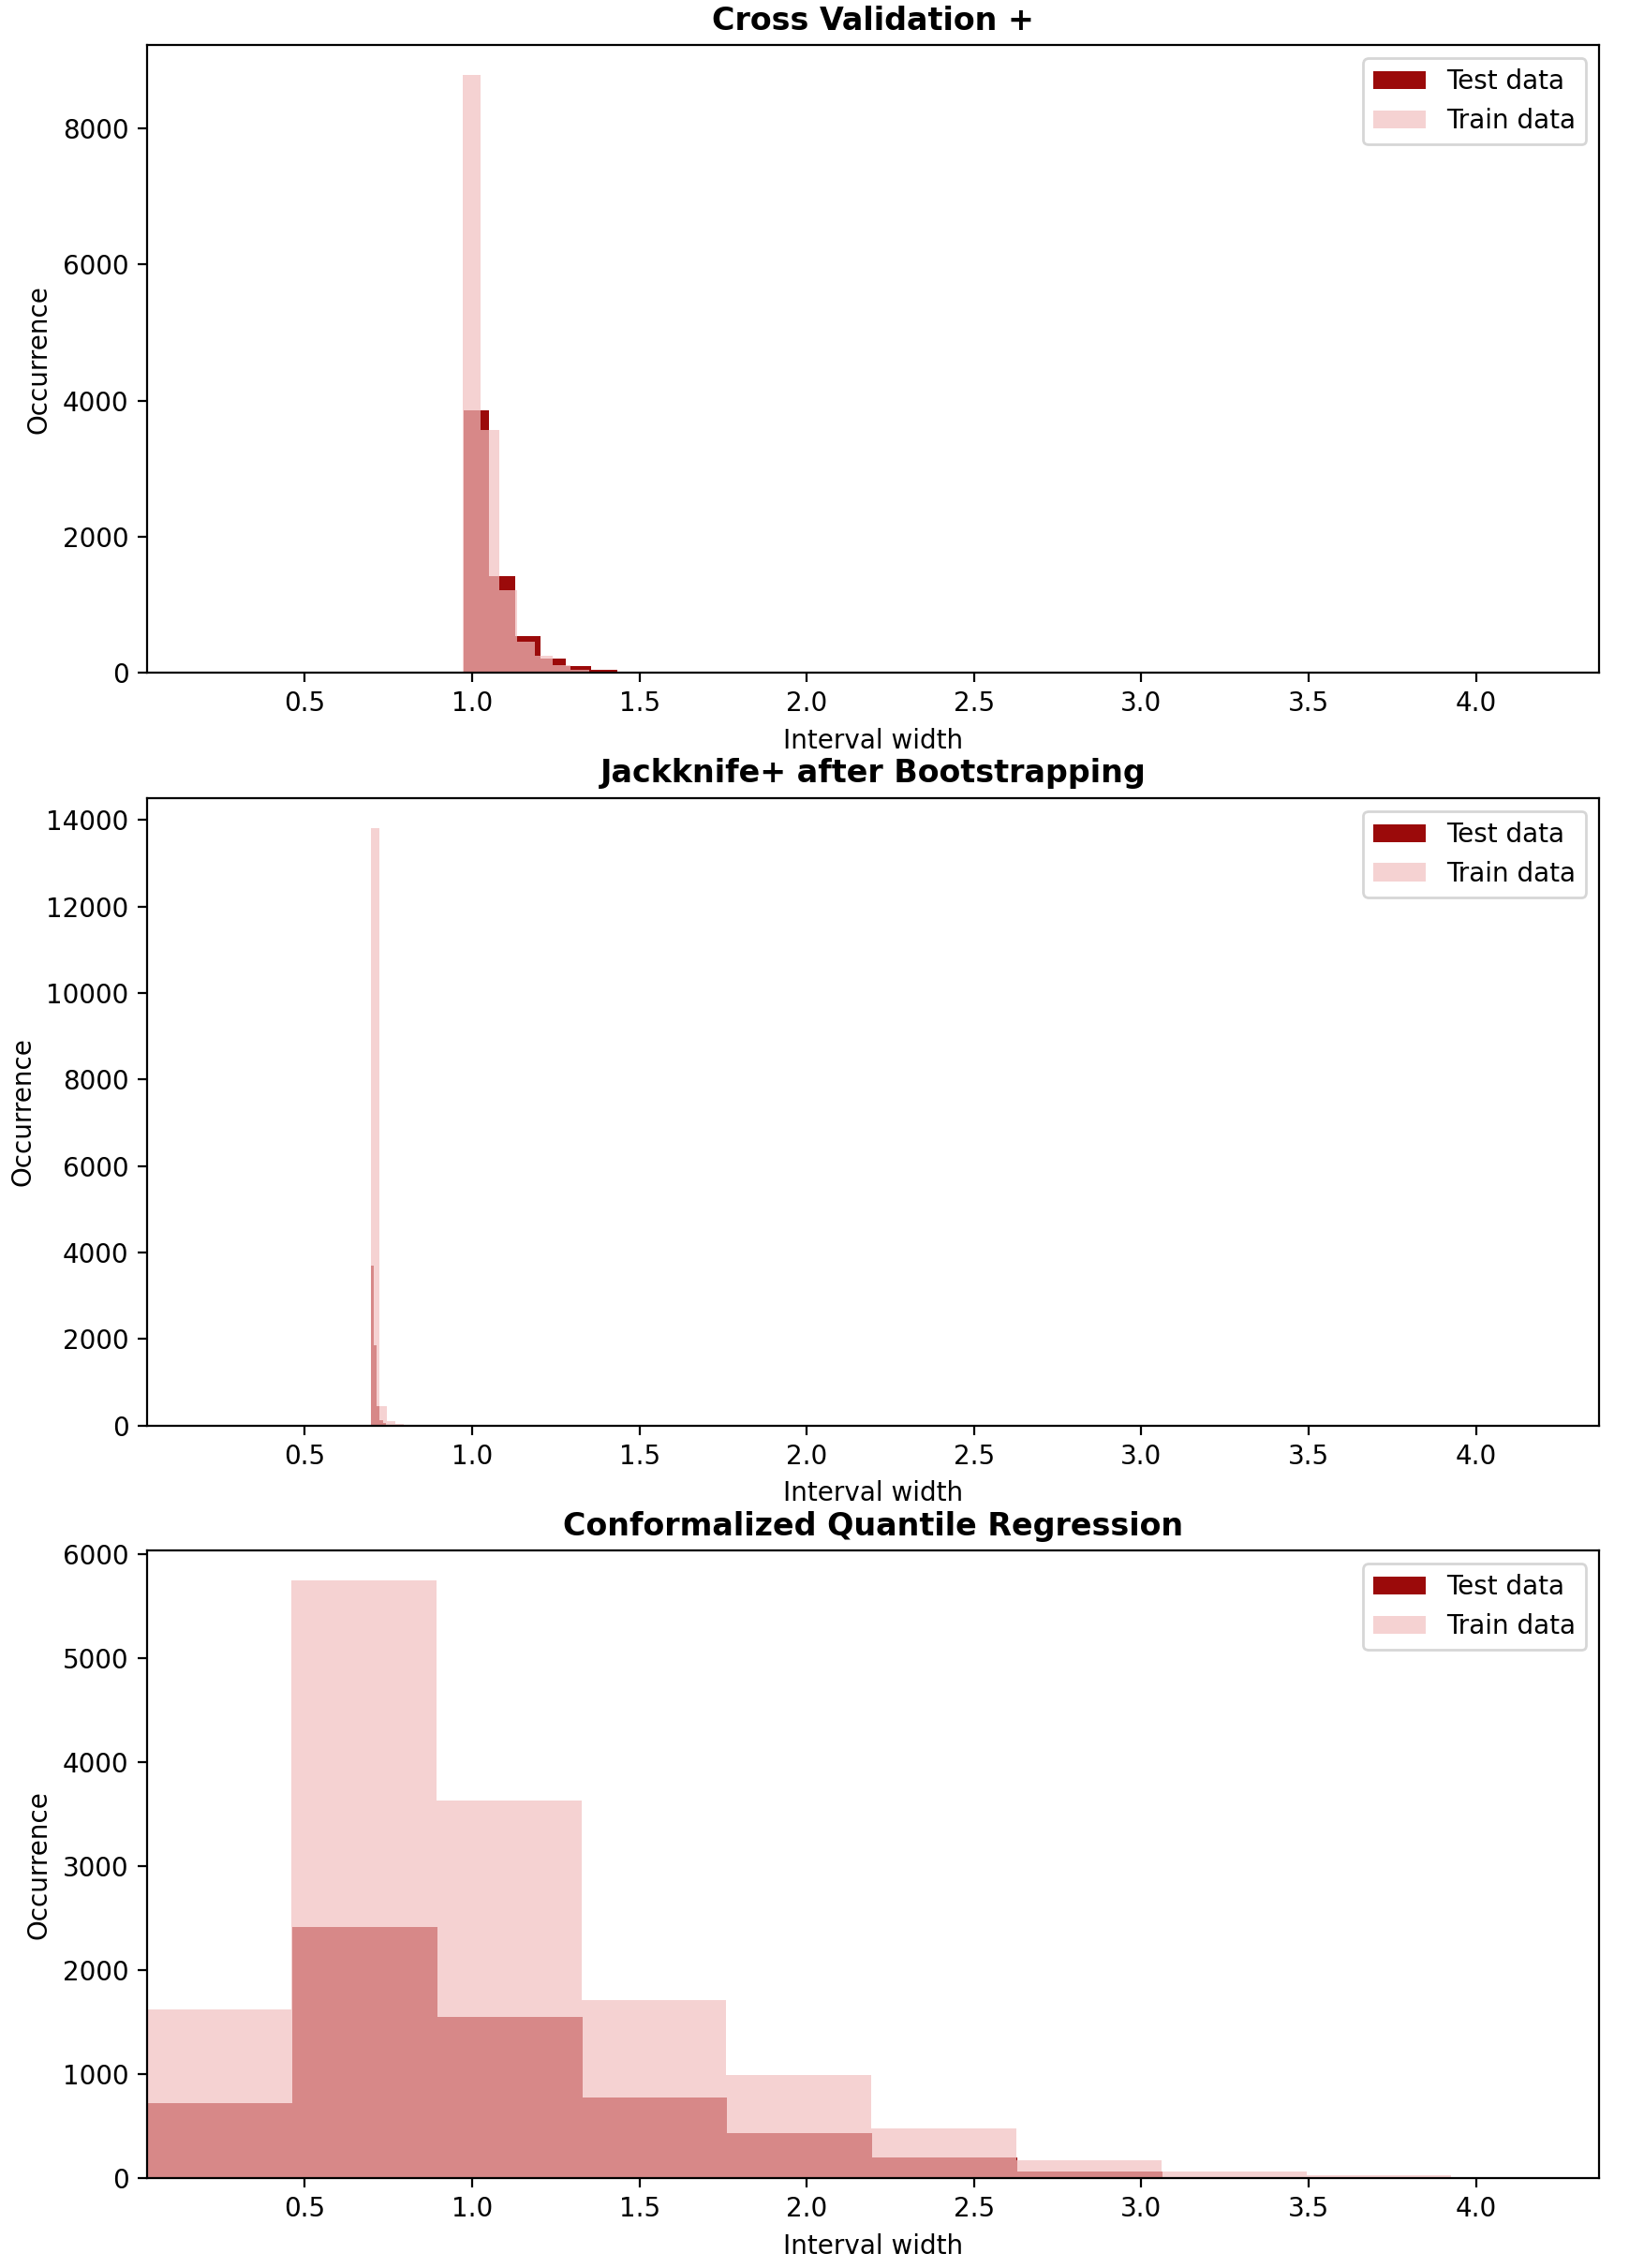
\includegraphics[width=1.15\textwidth, height=2.15\textwidth]{Figures/regression/width-occurrence-regression-problem.png}
        \caption{Intervals' width histograms}
        \label{subfig:regression-width-histograms}
    \end{subfigure}
    \hfill
    \begin{subfigure}[b]{0.32\textwidth}
        \centering
        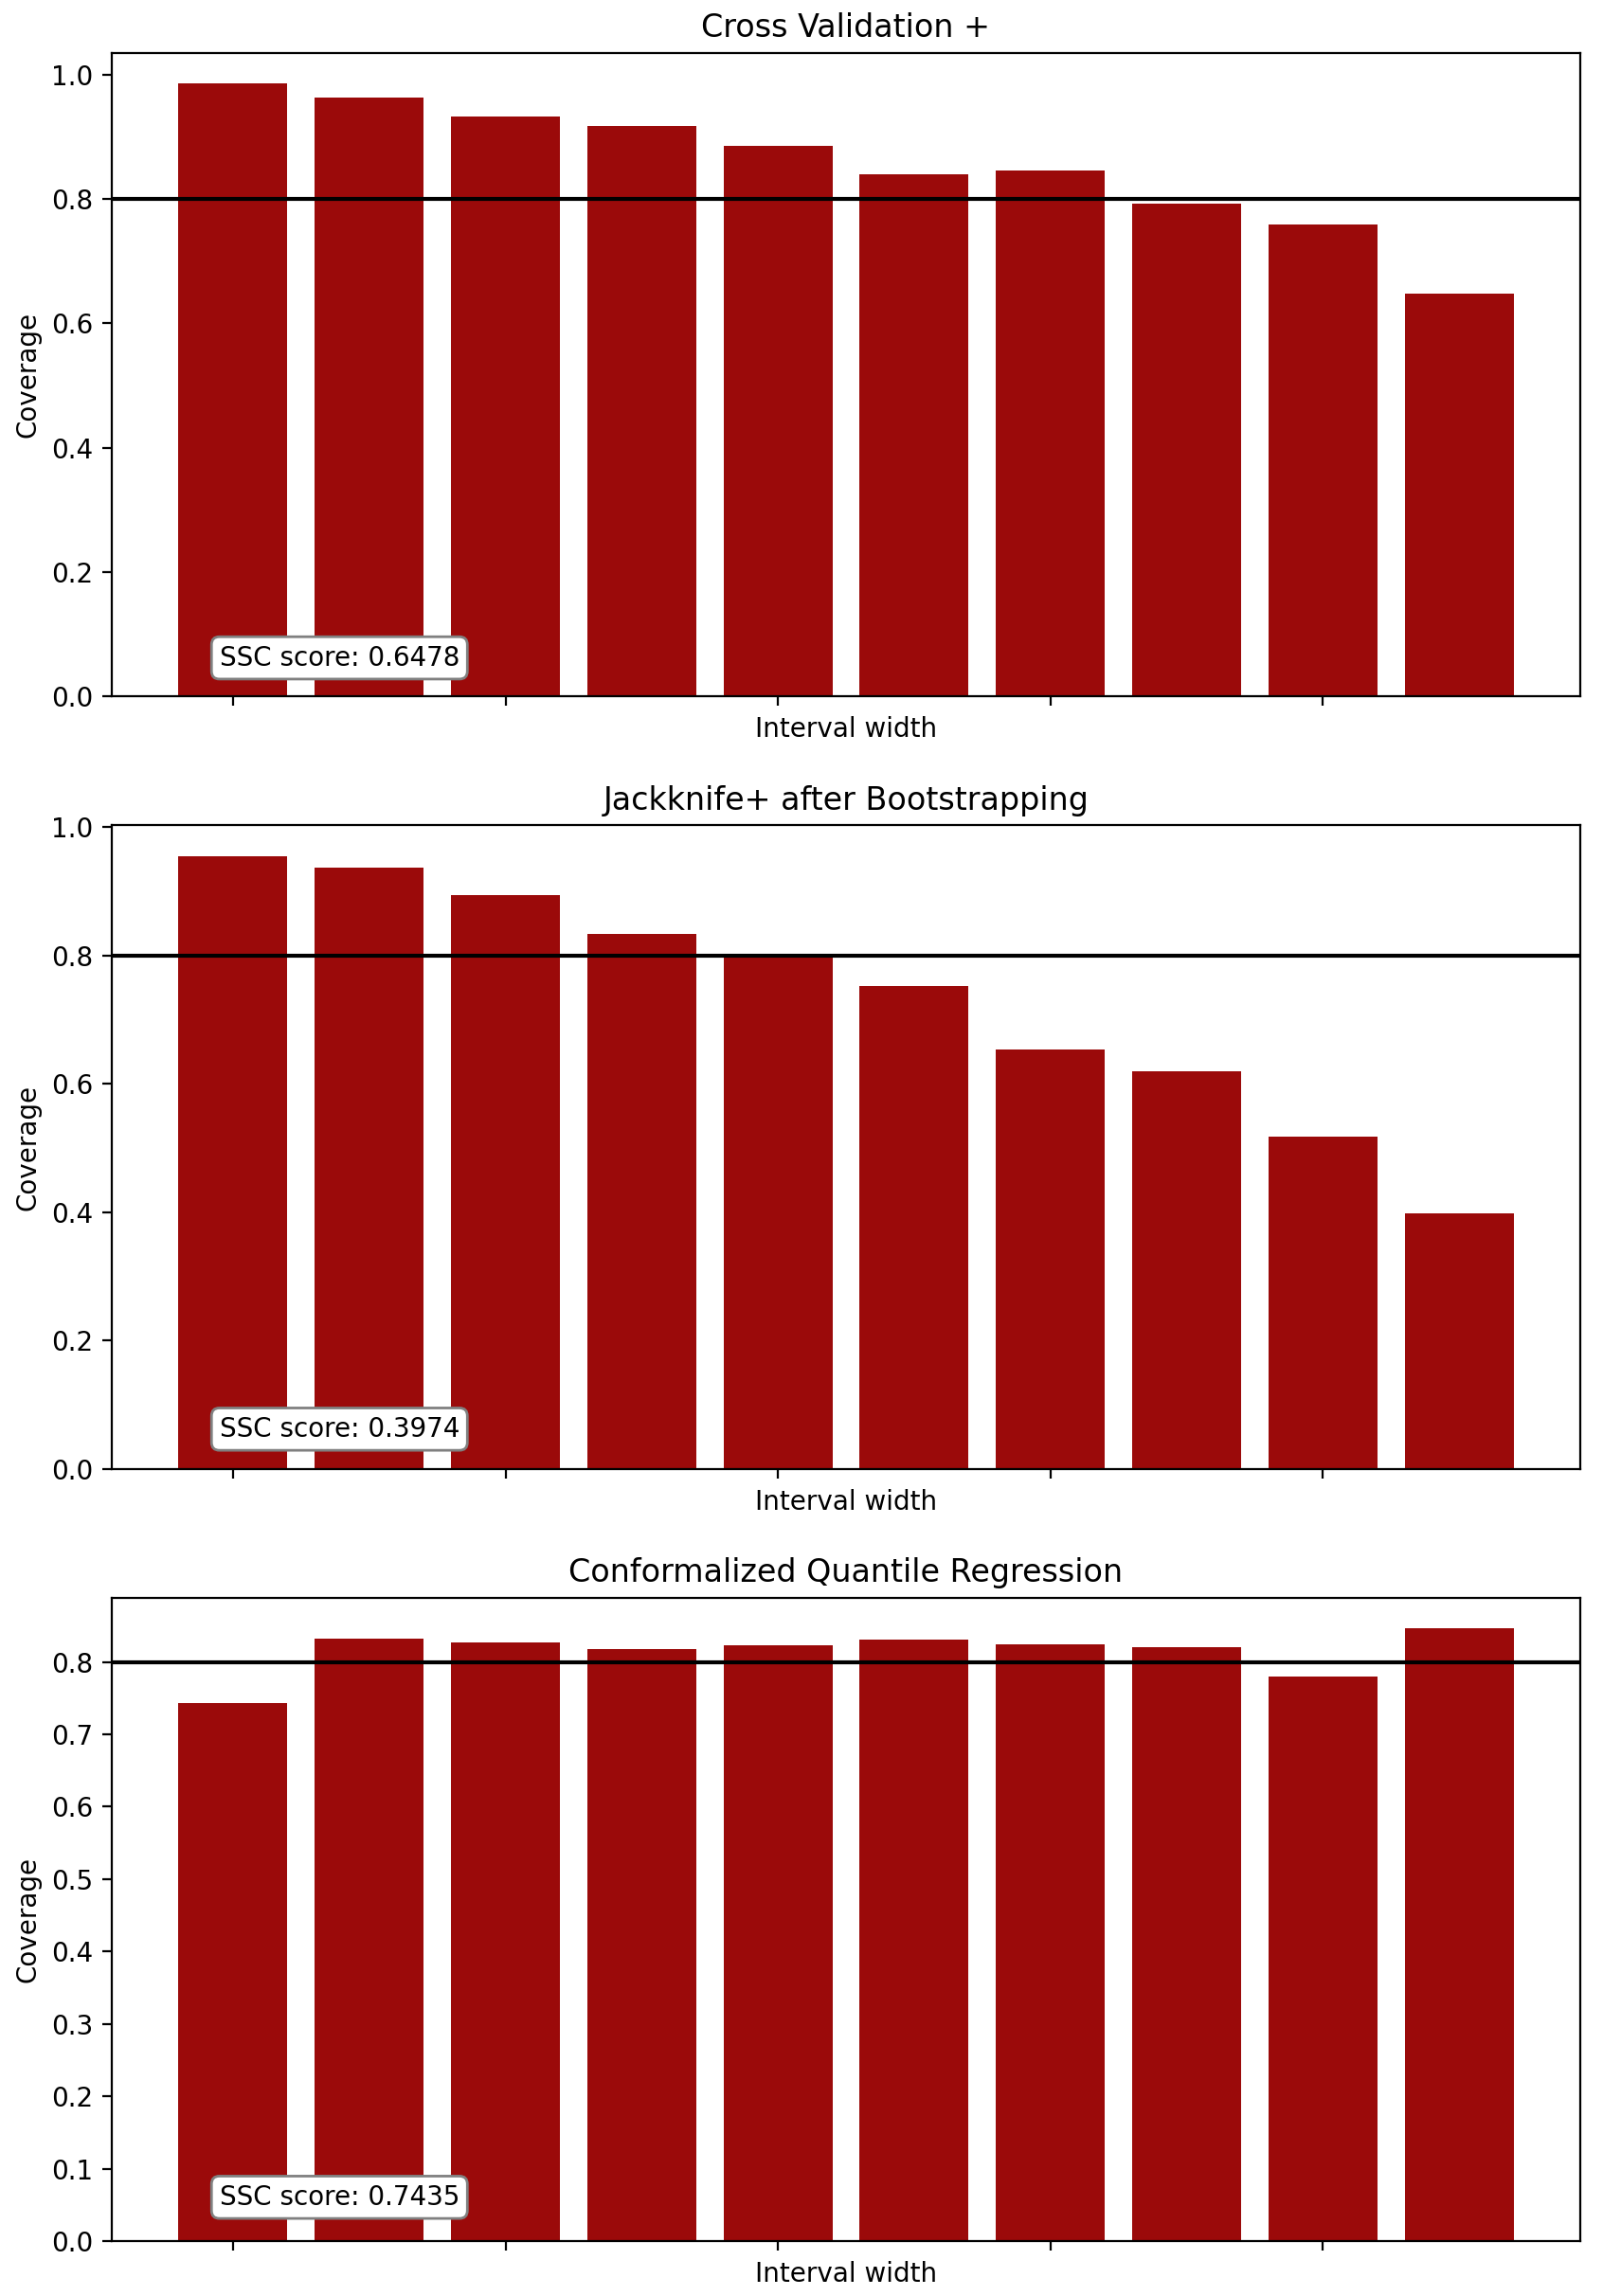
\includegraphics[width=1.15\textwidth, height=2.05\textwidth]{Figures/regression/coverage-vs-width-regression-problem.png}
        \caption{Coverage in function of intervals' width}
        \label{subfig:regression-coverage-width}
    \end{subfigure}
    \hfill % adds horizontal space between figures
    \begin{subfigure}[b]{0.32\textwidth} % Adjust the width to fit your needs
        \centering
        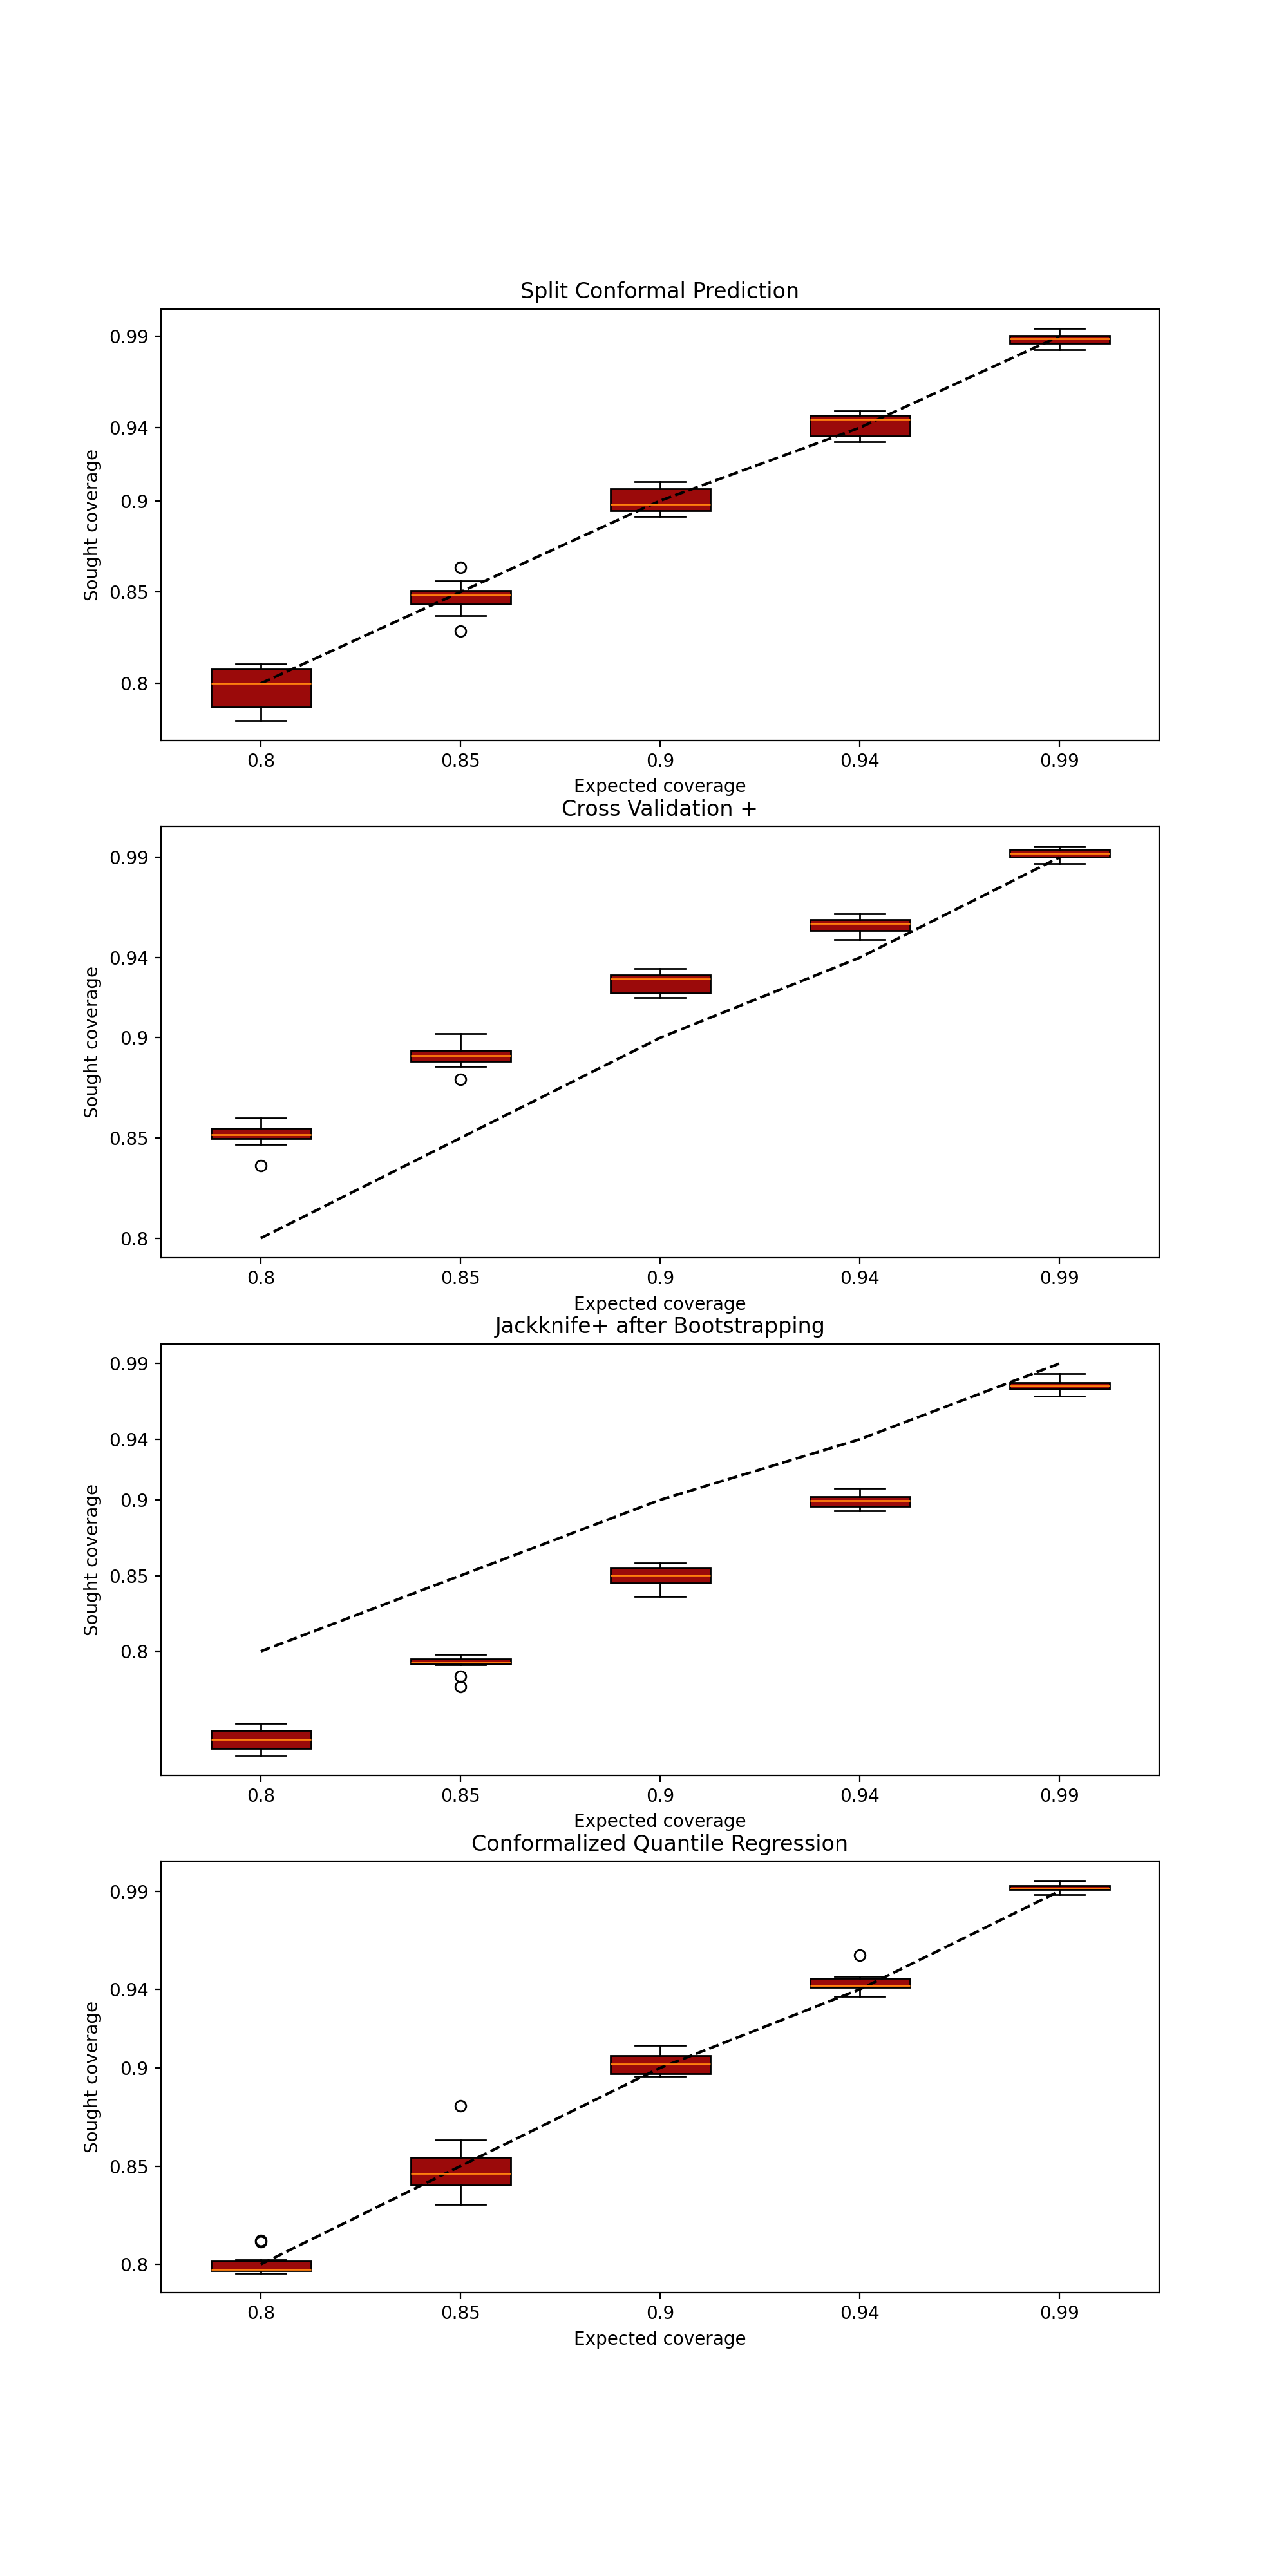
\includegraphics[width=1.15\textwidth, height=3\textwidth]{Figures/regression/coverage-vs-alpha-regression-problem.png} % Adjust the filename and path
        \caption{Coverage in function of $\a$}
        \label{subfig:regression-coverage-alpha}
    \end{subfigure}
    \caption{Visualizations related to width \& coverage distributions for the test data and 4 different strategies, from top to bottom: SCP, CV$+$, J$+$aB \& CQR. The first 2 plots just display the last 3 strategies, since SCP displays no adaptability at all (whereas J$+$aB slight to none adaptability).}
    \label{fig:regression-width-coverage}
\end{figure}

\section{Time series data}\label{sec:results-ts}

For the non-exchangeable data use-case, the same dataset as the \href{https://mapie.readthedocs.io/en/stable/examples_regression/4-tutorials/plot_ts-tutorial.html}{\texttt{mapie}'s time series tutorial} was chosen. This is the Victoria electricity demand dataset, used in the book “\textit{Forecasting: Principles and Practice}” (\cite{hyndman}), and contains a total of 1340 hourly samples. It deals with an electricity demand forecasting problem, which not only features daily and weekly seasonality, but it is also impacted by temperature. Thus, apart from the demand lagged up to 7 days (and other time features), temperature will be used as exogenous variable.

The dataset can be visualized in Figure \ref{fig:app-timeseries-data} at Appendix \ref{app:timeseries-original-problem}, where the complete set of visualizations and plots for the results' analysis can also be found.\\

In this case, a different ensemble model than gradient boosting (section \ref{sec:results-exchangeable}) is chosen as base estimator; in particular, a random forest regressor is implemented through \texttt{sklearn} library's \href{https://scikit-learn.org/stable/modules/generated/sklearn.ensemble.RandomForestRegressor.html}{\texttt{sklearn.ensemble.RandomForestRegressor}} Python class. 

Similarly to section \ref{sec:results-exchangeable}, a randomized grid-search is implemented using a 5-fold cross-validation to automate the hyper-parameters fine-tuning task. For this particular problem, the found best settings are:
\begin{itemize}
    \setlength{\itemsep}{0pt}
    \item \texttt{max\_{}depth}: $23$
    \item \texttt{n\_{}estimators}: $99$
\end{itemize}

Then, 2 strategies based in \texttt{mapie}'s \texttt{EnbPI} implementation (see the configuration at section \ref{sec:implementation}) are implemented, these are: \texttt{EnbPI} without partial fit (EnbPI\_{}nP), \textit{i.e.} the test residuals are not used to further adjust the model (steps 15-19 of Algorithm \ref{alg:EnbPI}); and \texttt{EnbPI} with partial fit (EnbPI).

In both cases, the prediction batches were implemented using the \texttt{mapie}'s class for bootstrapping blocks of data, \href{https://mapie.readthedocs.io/en/latest/generated/mapie.subsample.BlockBootstrap.html}{\texttt{mapie.subsample.BlockBootstrap}}, with:
\begin{itemize}
    \setlength{\itemsep}{0pt}
    \item \texttt{n\_{}resamplings}$=100$
    \item \texttt{length}$=48$ (i.e. batch size of $s=48\ \mathrm{h}$ samples).
\end{itemize}

All the code used to generate these results and visualizations can be found at the author's \href{https://github.com/gcastro-98/conformal-prediction/blob/main/timeseries.ipynb}{timeseries.ipynb} notebook.

\subsection{Original dataset}\label{subsec:timeseries-original}

For the original Victoria electricity demand dataset, both EnbPI\_{}nP and EnbPI are able to provide informative prediction intervals, presenting some minor differences in their attributes as shown in Table \ref{tab:timeseries-metrics}.

\begin{table}[ht]
\centering

\begin{subtable}{.5\textwidth}
    \hspace{-28mm}
    \begin{tabular}{|c|c|c|c|}
    \rowcolor{ColHead}\textcolor{white}{Strategy} & \textcolor{white}{Coverage} & \textcolor{white}{RMSE} & \textcolor{white}{Total time  (train $+$ infer)} \\ \hline
    \cellcolor{RowHead}EnbPI\_{}nP & 0.780 $\pm$ 0.069 & 0.165 $\pm$ 0.067 & 6.157 $\pm$ 0.334 \\
    \cellcolor{RowHead}EnbPI & 0.789 $\pm$ 0.058 & 0.165 $\pm$ 0.067 & 528.343 $\pm$ 0.359\\
    \hline
    \end{tabular}
\caption{Coverage, RMSE, total time (training \& inference with residuals adjustment if applies).}
\label{subtab:timeseries-metrics-1}
\end{subtable}

\begin{subtable}{.5\textwidth}
    \hspace{-28mm}
    \begin{tabular}{|c|c|c|c|c|}
    \rowcolor{ColHead}\textcolor{white}{Strategy} & \textcolor{white}{Coverage} & \textcolor{white}{Width} & \textcolor{white}{CWC} & \textcolor{white}{SSC} \\ \hline
    \cellcolor{RowHead}EnbPI\_{}nP & 0.780 $\pm$ 0.069 & 0.293 $\pm$ 0.013 & 0.935 $\pm$ 0.018 & ---  \\
    \cellcolor{RowHead}EnbPI & 0.789 $\pm$ 0.058 & 0.300 $\pm$ 0.007 & 0.934 $\pm$ 0.016 & 0.518 $\pm$ 0.209\\
    \hline
    \end{tabular}
\caption{Coverage, width, coverage width-based criterion (CWC) score \& size-stratified coverage (SSC) score}
\label{subtab:timeseries-metrics-2}
\end{subtable}

\caption{Different strategies' metrics after the Figure \ref{fig:ts-5-folds}'s 5-fold cross-validation for the time series problem with $\a=0.2$.}
\label{tab:timeseries-metrics}
\end{table}

Note these results stem from a 5-fold cross-validation, with the batches (not shuffled samples, to break temporal auto-correlation) shown in Figure \ref{fig:ts-5-folds}.

\begin{figure}[ht]
    %\centering
    \hspace{-10mm}
    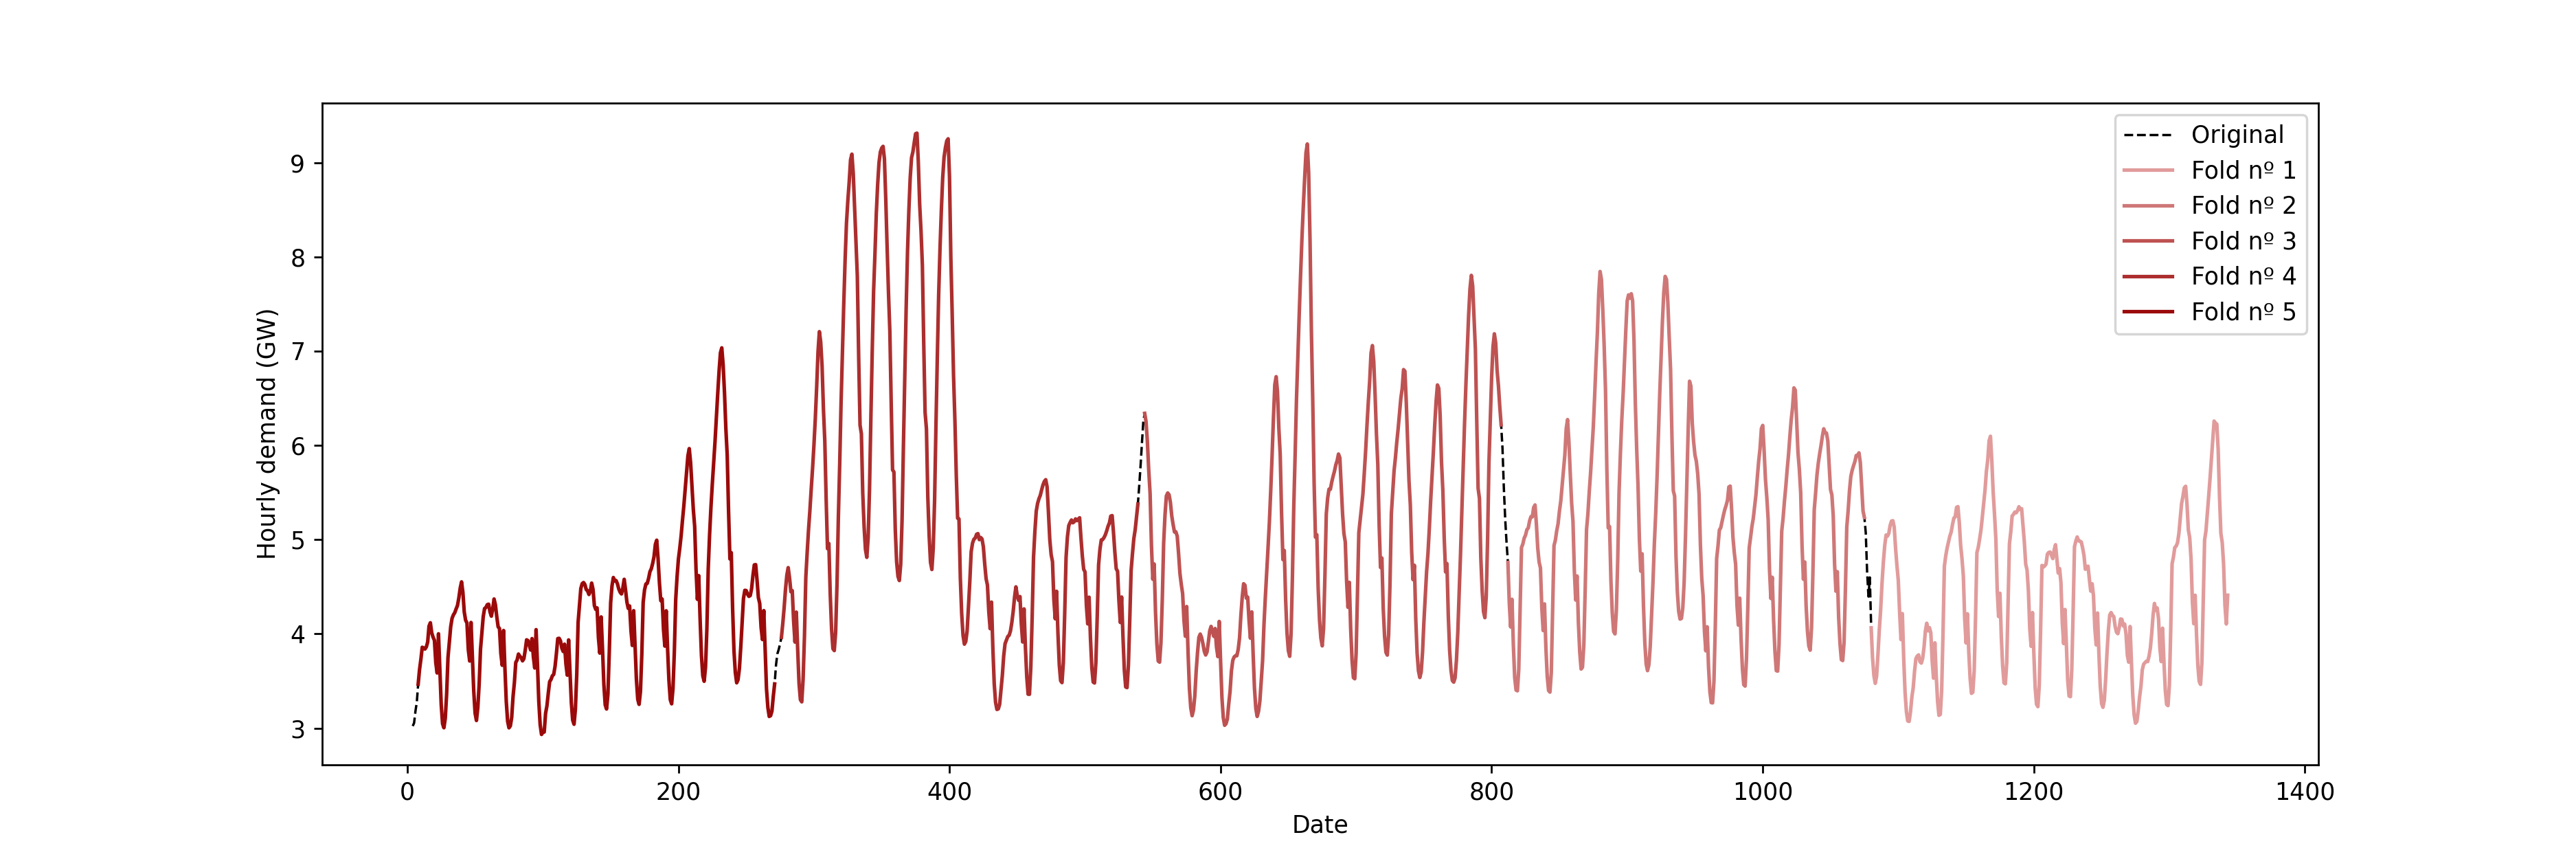
\includegraphics[width=1.15\textwidth]{Figures/timeseries/without-change-point/ts-5-folds.png}
    \caption{5-fold splits from the original dataset.}
    \label{fig:ts-5-folds}
\end{figure}

In particular, it is easy to conclude the benefits of adjusting the intervals with the test residuals (steps 15-19 of Algorithm \ref{alg:EnbPI}) since EnbPI is better than EnbPI\_{}nP. Despite a slight $0.001$ loss width-coverage ratio score, the global coverage improved. Not only global coverage was improved, but also adaptive intervals were enabled achieving a $0.518\pm 0.209$ SSC score (with respect to the non-adaptive intervals of EnbPI\_{}nP).

The latter can be easily checked in sub-figures \ref{subfig:timeseries-width-histograms} \& \ref{subfig:timeseries-coverage-width}, where not only EnbPI features several sized intervals, but it also attains uniform coverage in every of them (and almost the expected one). Also, the ability to attain global coverage for different $\a$ values is shown in sub-figure \ref{subfig:timeseries-coverage-alpha}.

\begin{figure}[ht]
    \centering
    %\hspace{-10mm}
    \begin{subfigure}[b]{0.32\textwidth}
        \centering
        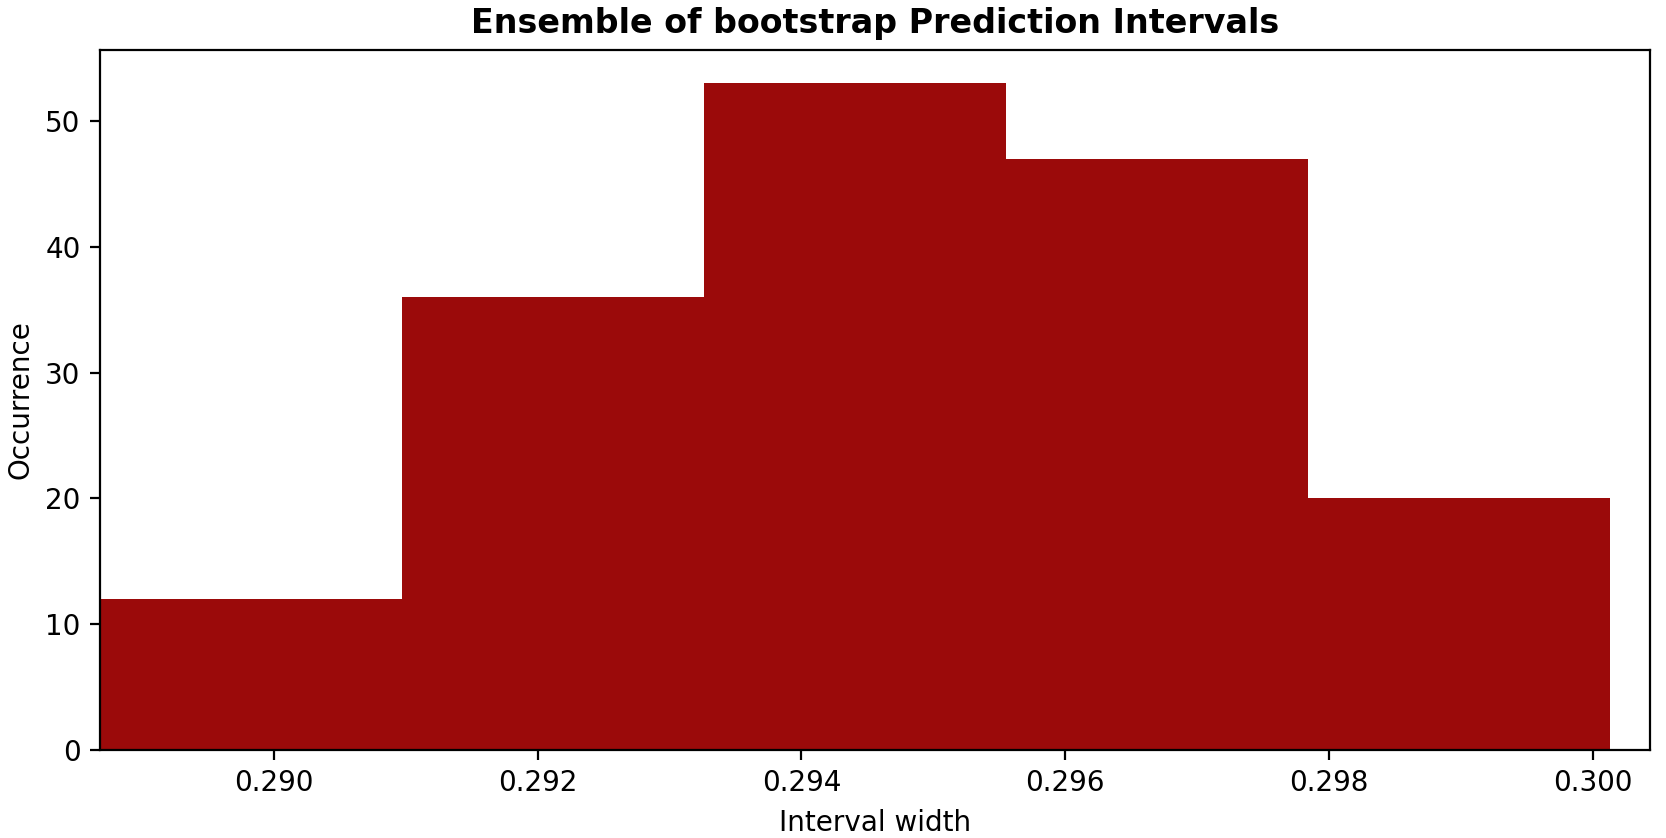
\includegraphics[width=1.05\textwidth, height=0.85\textwidth]{Figures/timeseries/without-change-point/width-occurrence-timeseries-problem.png}
        \caption{Intervals' width histograms}
        \label{subfig:timeseries-width-histograms}
    \end{subfigure}
    \hfill
    \begin{subfigure}[b]{0.32\textwidth}
        \centering
        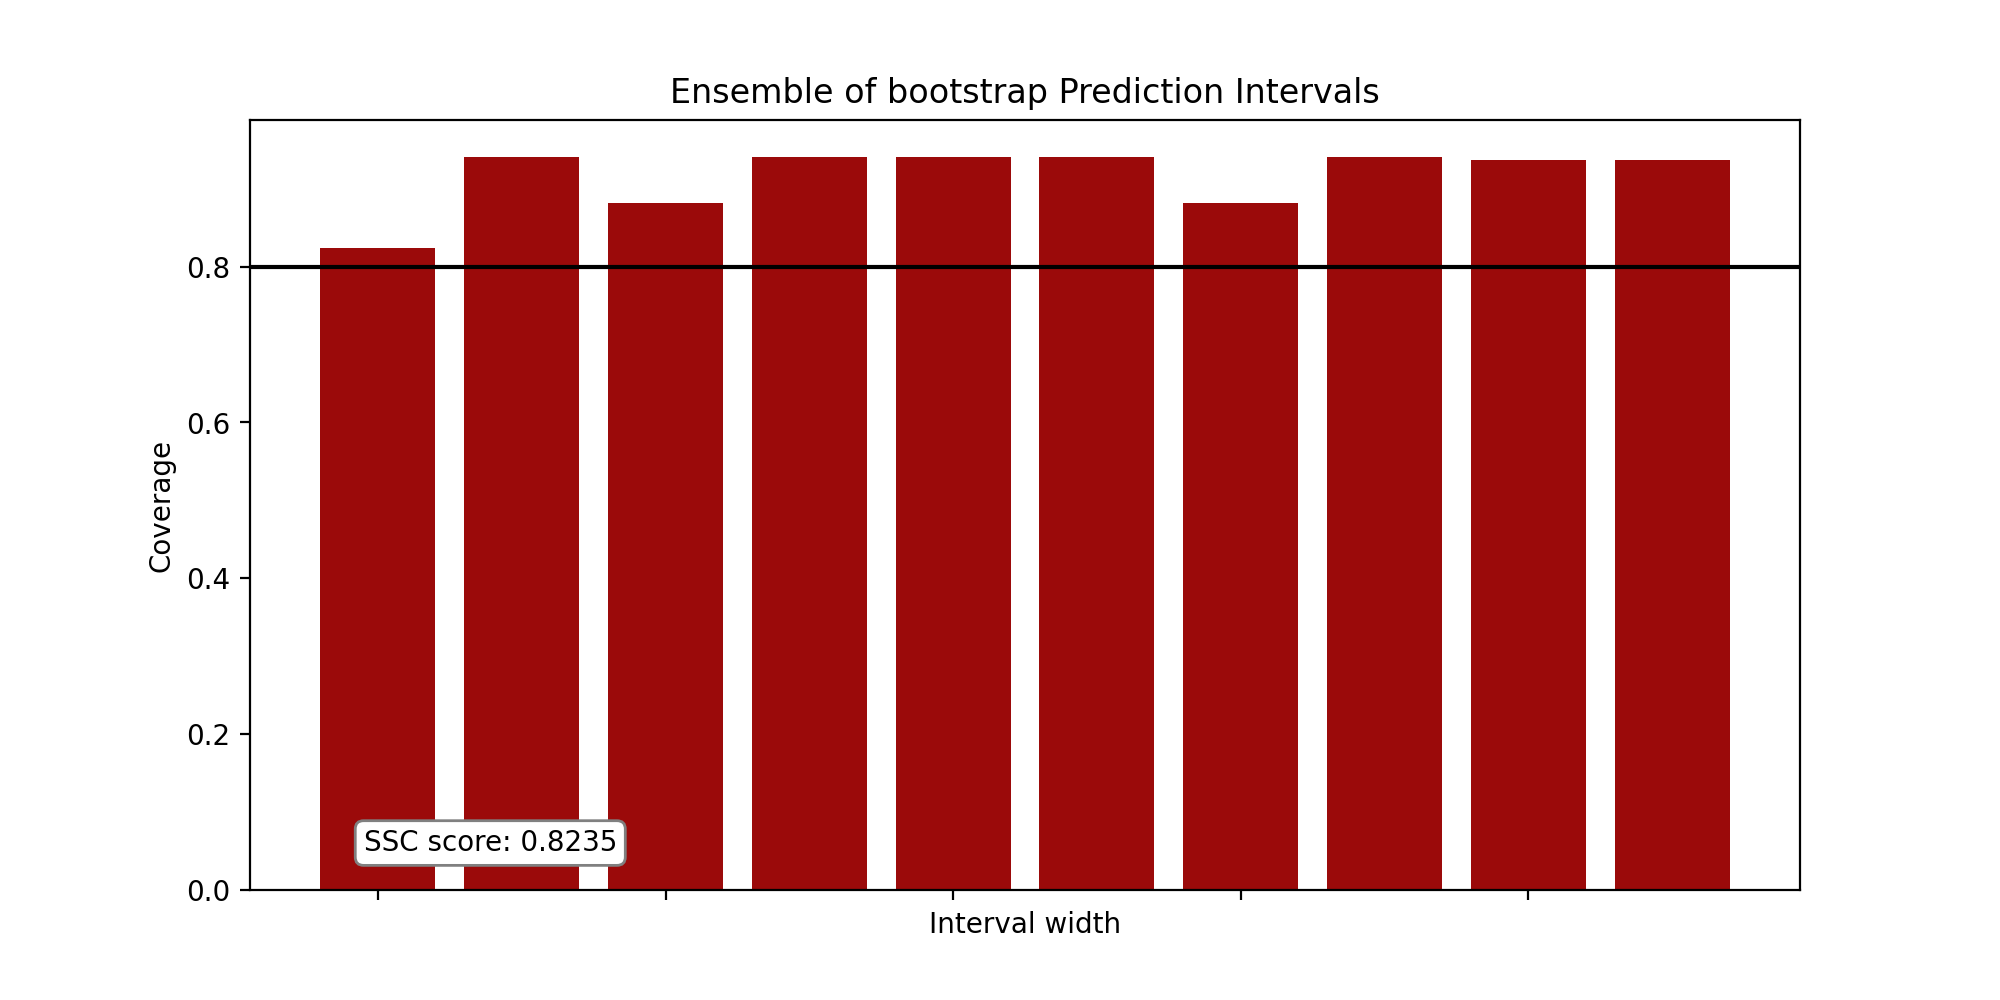
\includegraphics[width=1.15\textwidth, height=0.85\textwidth]{Figures/timeseries/without-change-point/coverage-vs-width-timeseries-problem.png}
        \caption{Coverage in function of intervals' width}
        \label{subfig:timeseries-coverage-width}
    \end{subfigure}
    \hfill % adds horizontal space between figures
    \begin{subfigure}[b]{0.32\textwidth} % Adjust the width to fit your needs
        \centering
        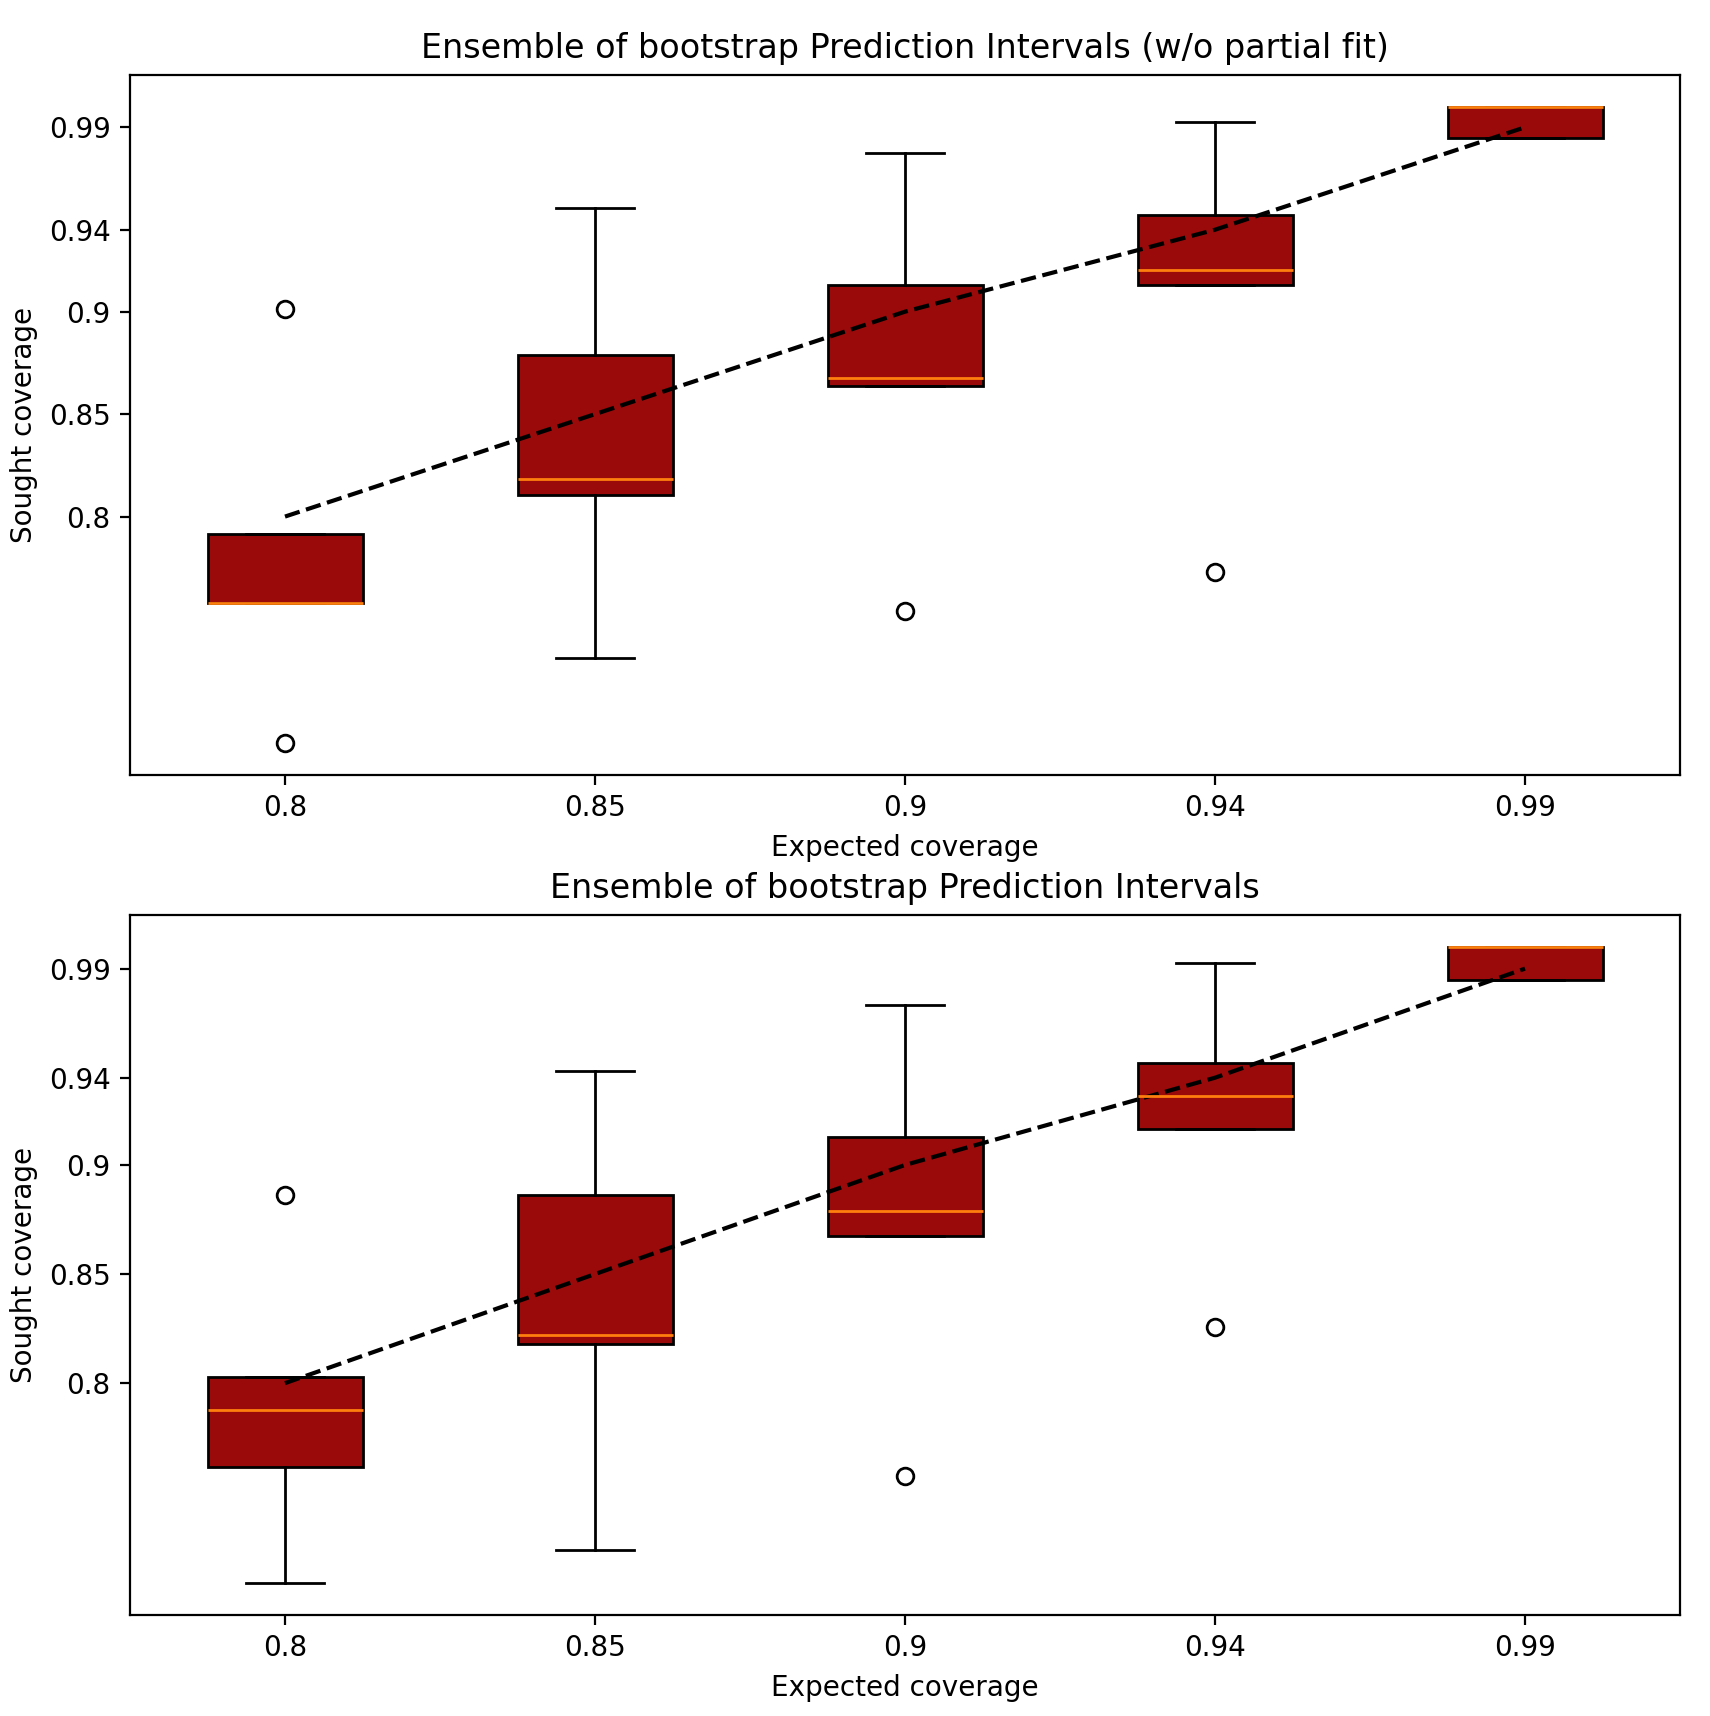
\includegraphics[width=1.15\textwidth, height=1.75\textwidth]{Figures/timeseries/without-change-point/coverage-vs-alpha-timeseries-problem.png} % Adjust the filename and path
        \caption{Coverage in function of $\a$}
        \label{subfig:timeseries-coverage-alpha}
    \end{subfigure}
    \caption{Intervals width \& coverage distributions for the test data and the EnbPI strategy (without partial fit, top; and with it, bottom).}
    \label{fig:timeseries-width-coverage}
\end{figure}

Of course, despite its complexity and multiple seasonality, this dataset is very consistent presenting almost neither trend nor strong distribution shifts as shown in Figure \ref{fig:ts-5-folds}. Due to this reason, EnbPI\_{}nP \& EnbPI performances are really similar.

To avoid outshining EnbPI adaptive ability, a special strong-shift case is presented in subsection \ref{subsec:ts-with-cpoint}.

\subsection{Change point in the test data}\label{subsec:ts-with-cpoint}

Henceforth in this subsection, a special case of the time series problem is considered. In particular, a change point will be added in the test split (by artificially subtracting $2\ \mathrm{GW}$) to mock off the situation in which there is a sudden strong distribution shift in the middle of the test data. Also, in this case and unless otherwise is specified, $\a=0.05$ is chosen as miscoverage level.

The dataset with this change point can be visualized in Figure \ref{fig:app-timeseries-data-cpoint} at Appendix \ref{app:timeseries-cpoint-problem} (where the rest of visualizations can also be found).\\

For this particular scenario, EnbPI\_{}nP and EnbPI do present significance differences in their performance, as shown in Table \ref{tab:timeseries-metrics-cpoint}.

\begin{table}[ht]
\centering

\begin{subtable}{.5\textwidth}
    \hspace{-28mm}
    \begin{tabular}{|c|c|c|c|}
    \rowcolor{ColHead}\textcolor{white}{Strategy} & \textcolor{white}{Coverage} & \textcolor{white}{RMSE} & \textcolor{white}{Total time (train $+$ infer)} \\ \hline
    \cellcolor{RowHead}EnbPI\_{}nP & 0.439 $\pm$ 0.075 & 1.431 $\pm$ 0.024 & 6.047 $\pm$ 0.307 \\
    \cellcolor{RowHead}EnbPI & 0.696 $\pm$ 0.042 & 1.431 $\pm$ 0.024 & 529.902 $\pm$ 1.319\\
    \hline
    \end{tabular}
\caption{Coverage, RMSE, total time (training \& inference with residuals adjustment if applies).}
\label{subtab:timeseries-metrics-1-cpoint}
\end{subtable}

\begin{subtable}{.5\textwidth}
    \hspace{-18mm}
    \begin{tabular}{|c|c|c|c|}
    \rowcolor{ColHead}\textcolor{white}{Strategy} & \textcolor{white}{Coverage} & \textcolor{white}{Width} %& \textcolor{white}{CWC} 
    & \textcolor{white}{SSC} \\ \hline
    \cellcolor{RowHead}EnbPI\_{}nP & 0.439 $\pm$ 0.075 & 0.569 $\pm$ 0.043 % & --- %0.899 $\pm$ 0.031 
    & ---  \\
    \cellcolor{RowHead}EnbPI & 0.696 $\pm$ 0.042 & 1.300 $\pm$ 0.034 % & --- %0.777 $\pm$ 0.060 
    & 0.069 $\pm$ 0.120\\
    \hline
    \end{tabular}
\caption{Coverage, width % , %coverage width-based criterion (CWC) score 
\& size-stratified coverage (SSC) score.}
\label{subtab:timeseries-metrics-2-cpoint}
\end{subtable}

\caption{Different strategies' metrics after the Figure \ref{fig:ts-5-folds-cpoint}'s 5-fold cross-validation for the time series problem (with a change point in test) and $\a=0.05$.}
\label{tab:timeseries-metrics-cpoint}
\end{table}

Note these metrics are obtained from the batched 5-fold cross-validation splits shown in Figure \ref{fig:ts-5-folds-cpoint} (just the test splits are shown, the train split is the rest of the dataset for each case).

\begin{figure}[ht]
    \hspace{-12mm}
    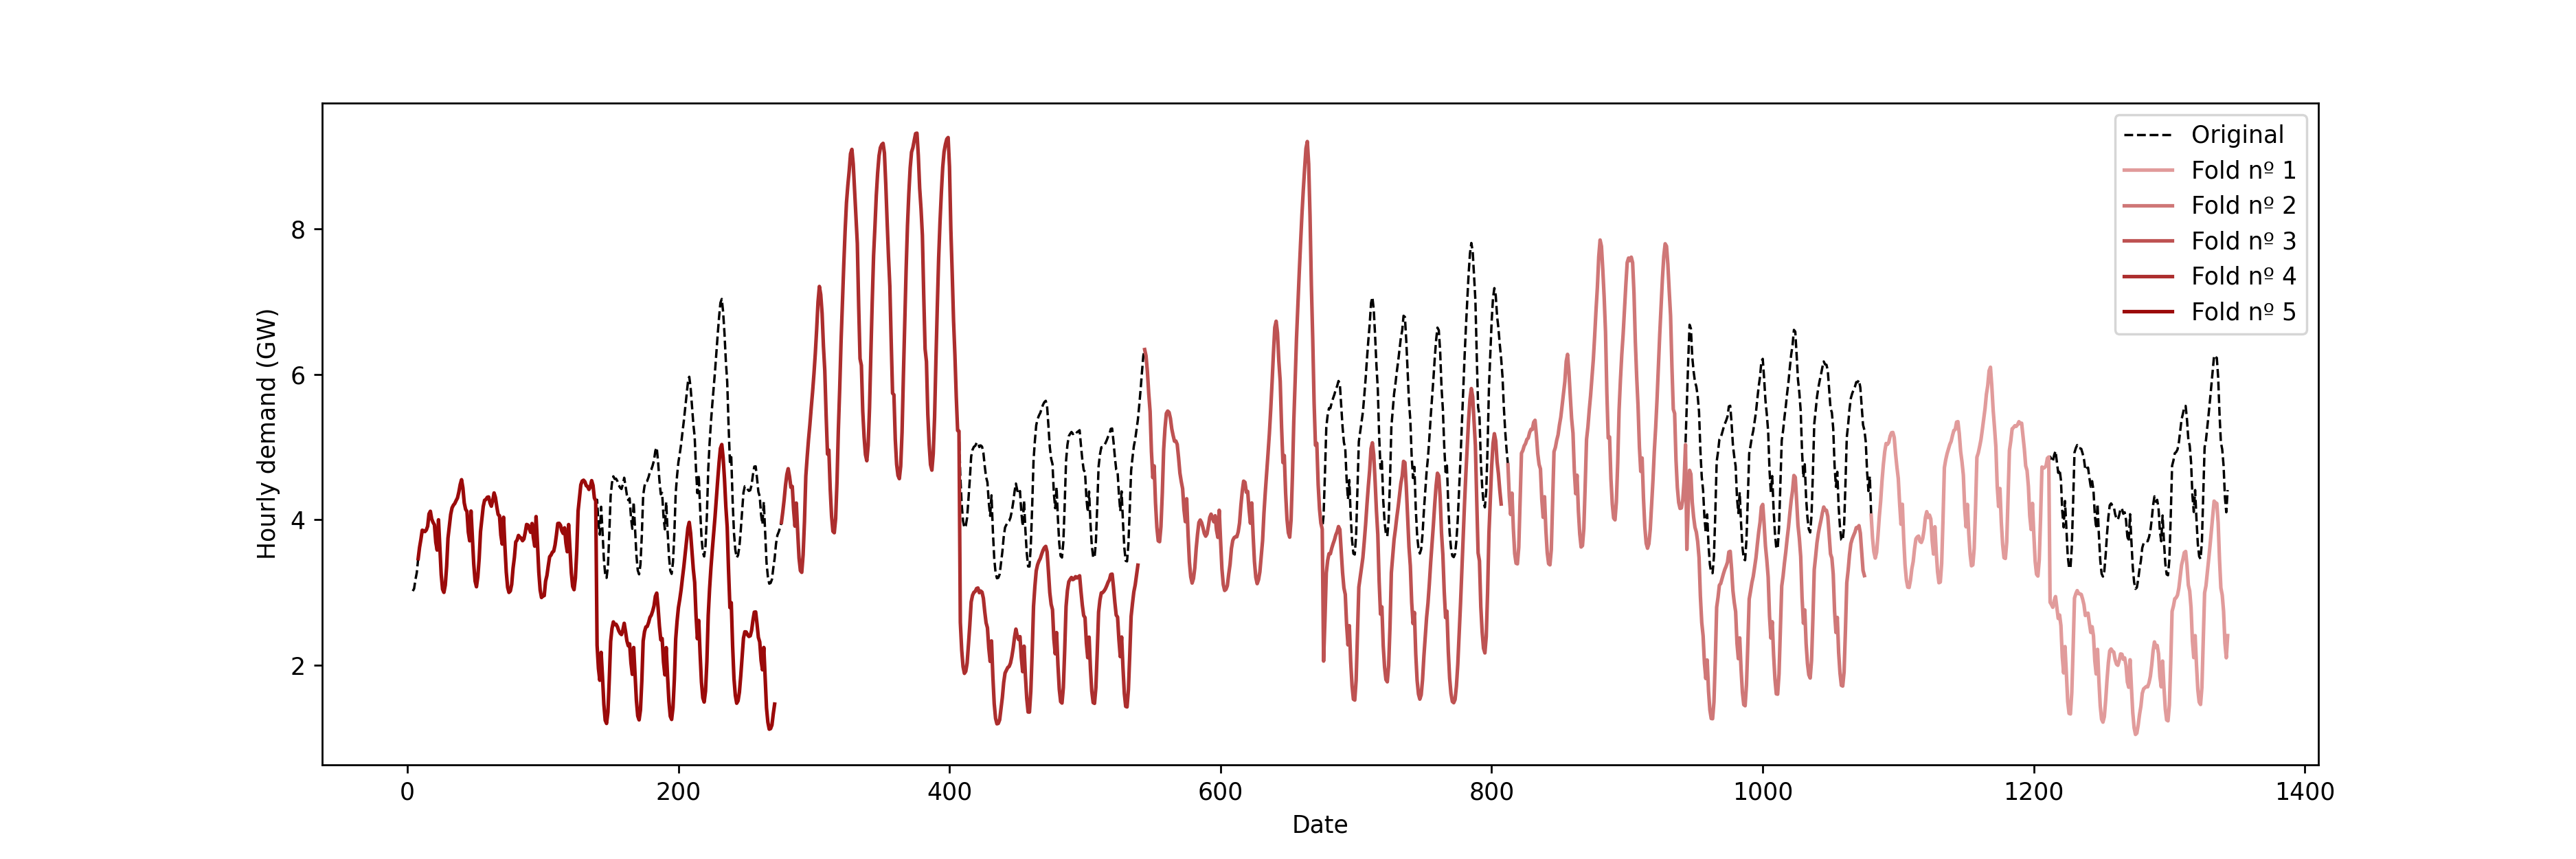
\includegraphics[width=1.15\textwidth]{Figures/timeseries/with-change-point/ts-with-change-point-5-folds.png}
    \caption{5-fold splits from the dataset with change point in the test split(s).}
    \label{fig:ts-5-folds-cpoint}
\end{figure}

These results clearly justify the need of adjusting the intervals with the test residuals (EnbPI) despite of significantly increasing the computational times.\\

Specifically, EnbPI's ability of increasing the intervals width after the strong-shift in the middle of the test split, allows the methodology to recover and yields a $58.54\%$ coverage increase. This justified need of suddenly increasing intervals width (making them less informative) is the reason why the CWC score is not shown in Table \ref{tab:timeseries-metrics-cpoint}, since it could lead to wrong interpretations (the metric would penalize this behavior).

This behavior by which EnbPI, and after the change point, tries to compensate the lack of coverage in their future predictions (by increasing intervals width) is easily observed at Figure \ref{fig:timeseries-prediction-intervals-cpoint}.\\

\begin{figure}[ht]
    \centering
    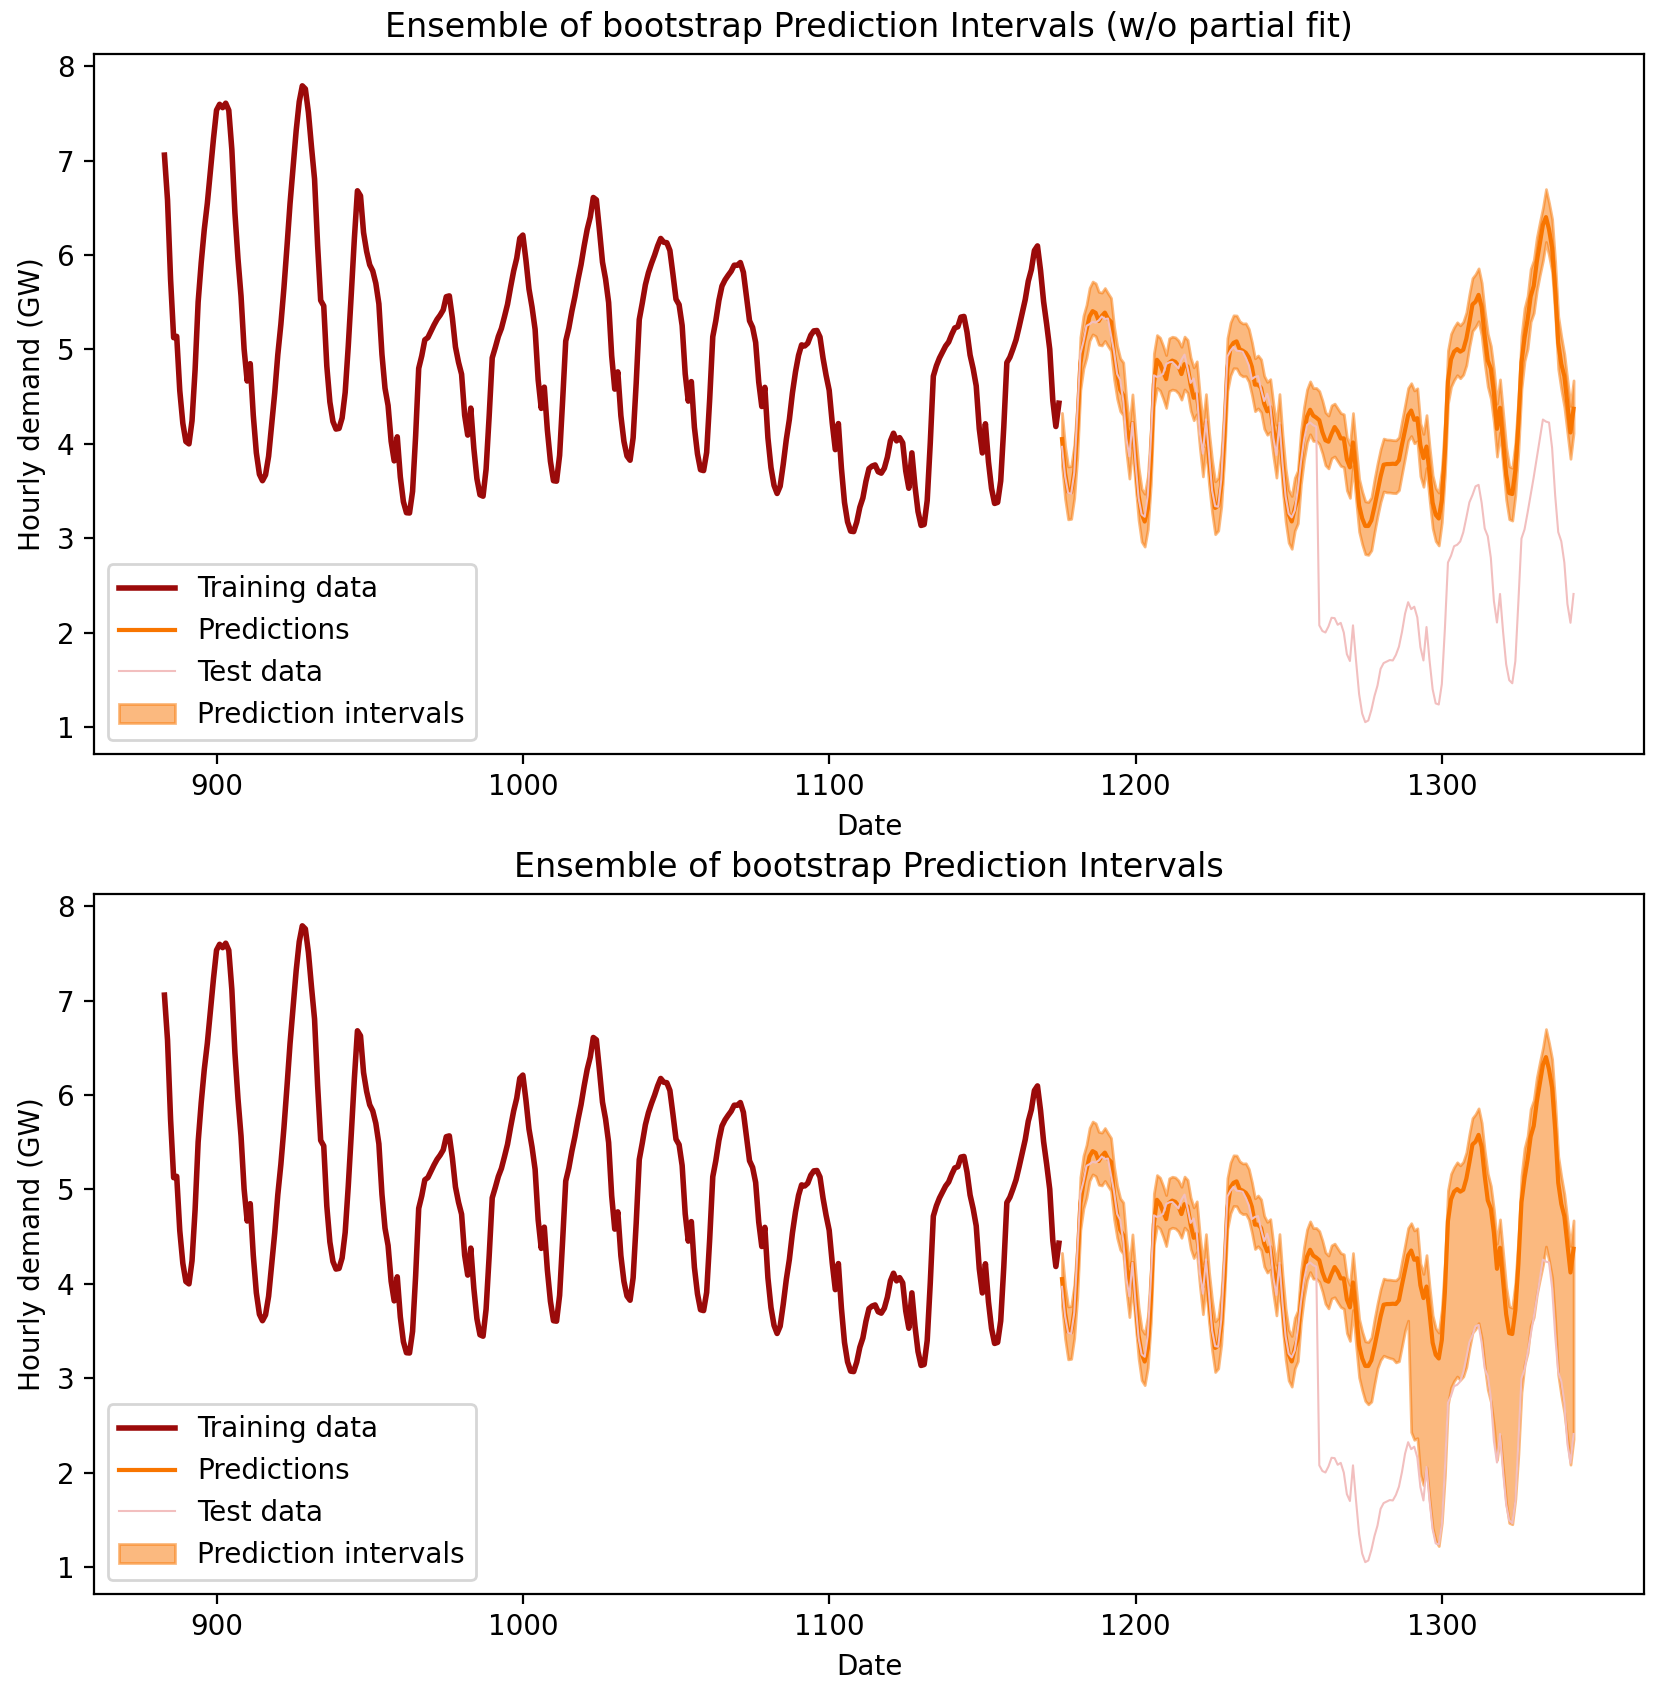
\includegraphics[width=\textwidth]{Figures/timeseries/with-change-point/prediction-intervals-timeseries-problem-with-change-point.png}
    \caption{EnbPI increasing interval width through its partial fit feature, for a particular experiment with $\a=0.05$.}
    \label{fig:timeseries-prediction-intervals-cpoint}
\end{figure}

However, note that this recover speed is directly related to the tolerated miscoverage level. Namely, the lower the miscoverage $\a$ level, the quicker this change will be featured. In particular, in Figure \ref{fig:timeseries-intervals-alpha-cpoint}, it can be seen how EnbPI has no time to recover for $\a=0.20, 0.15$ ($80\%$, $85\%$ confidence levels; top \& middle sub-figures), while it effectively does for $\a=0.10$ (but, of course, later than Figure \ref{fig:timeseries-prediction-intervals-cpoint}'s $\a=0.05$).

\begin{figure}[ht]
    \centering
    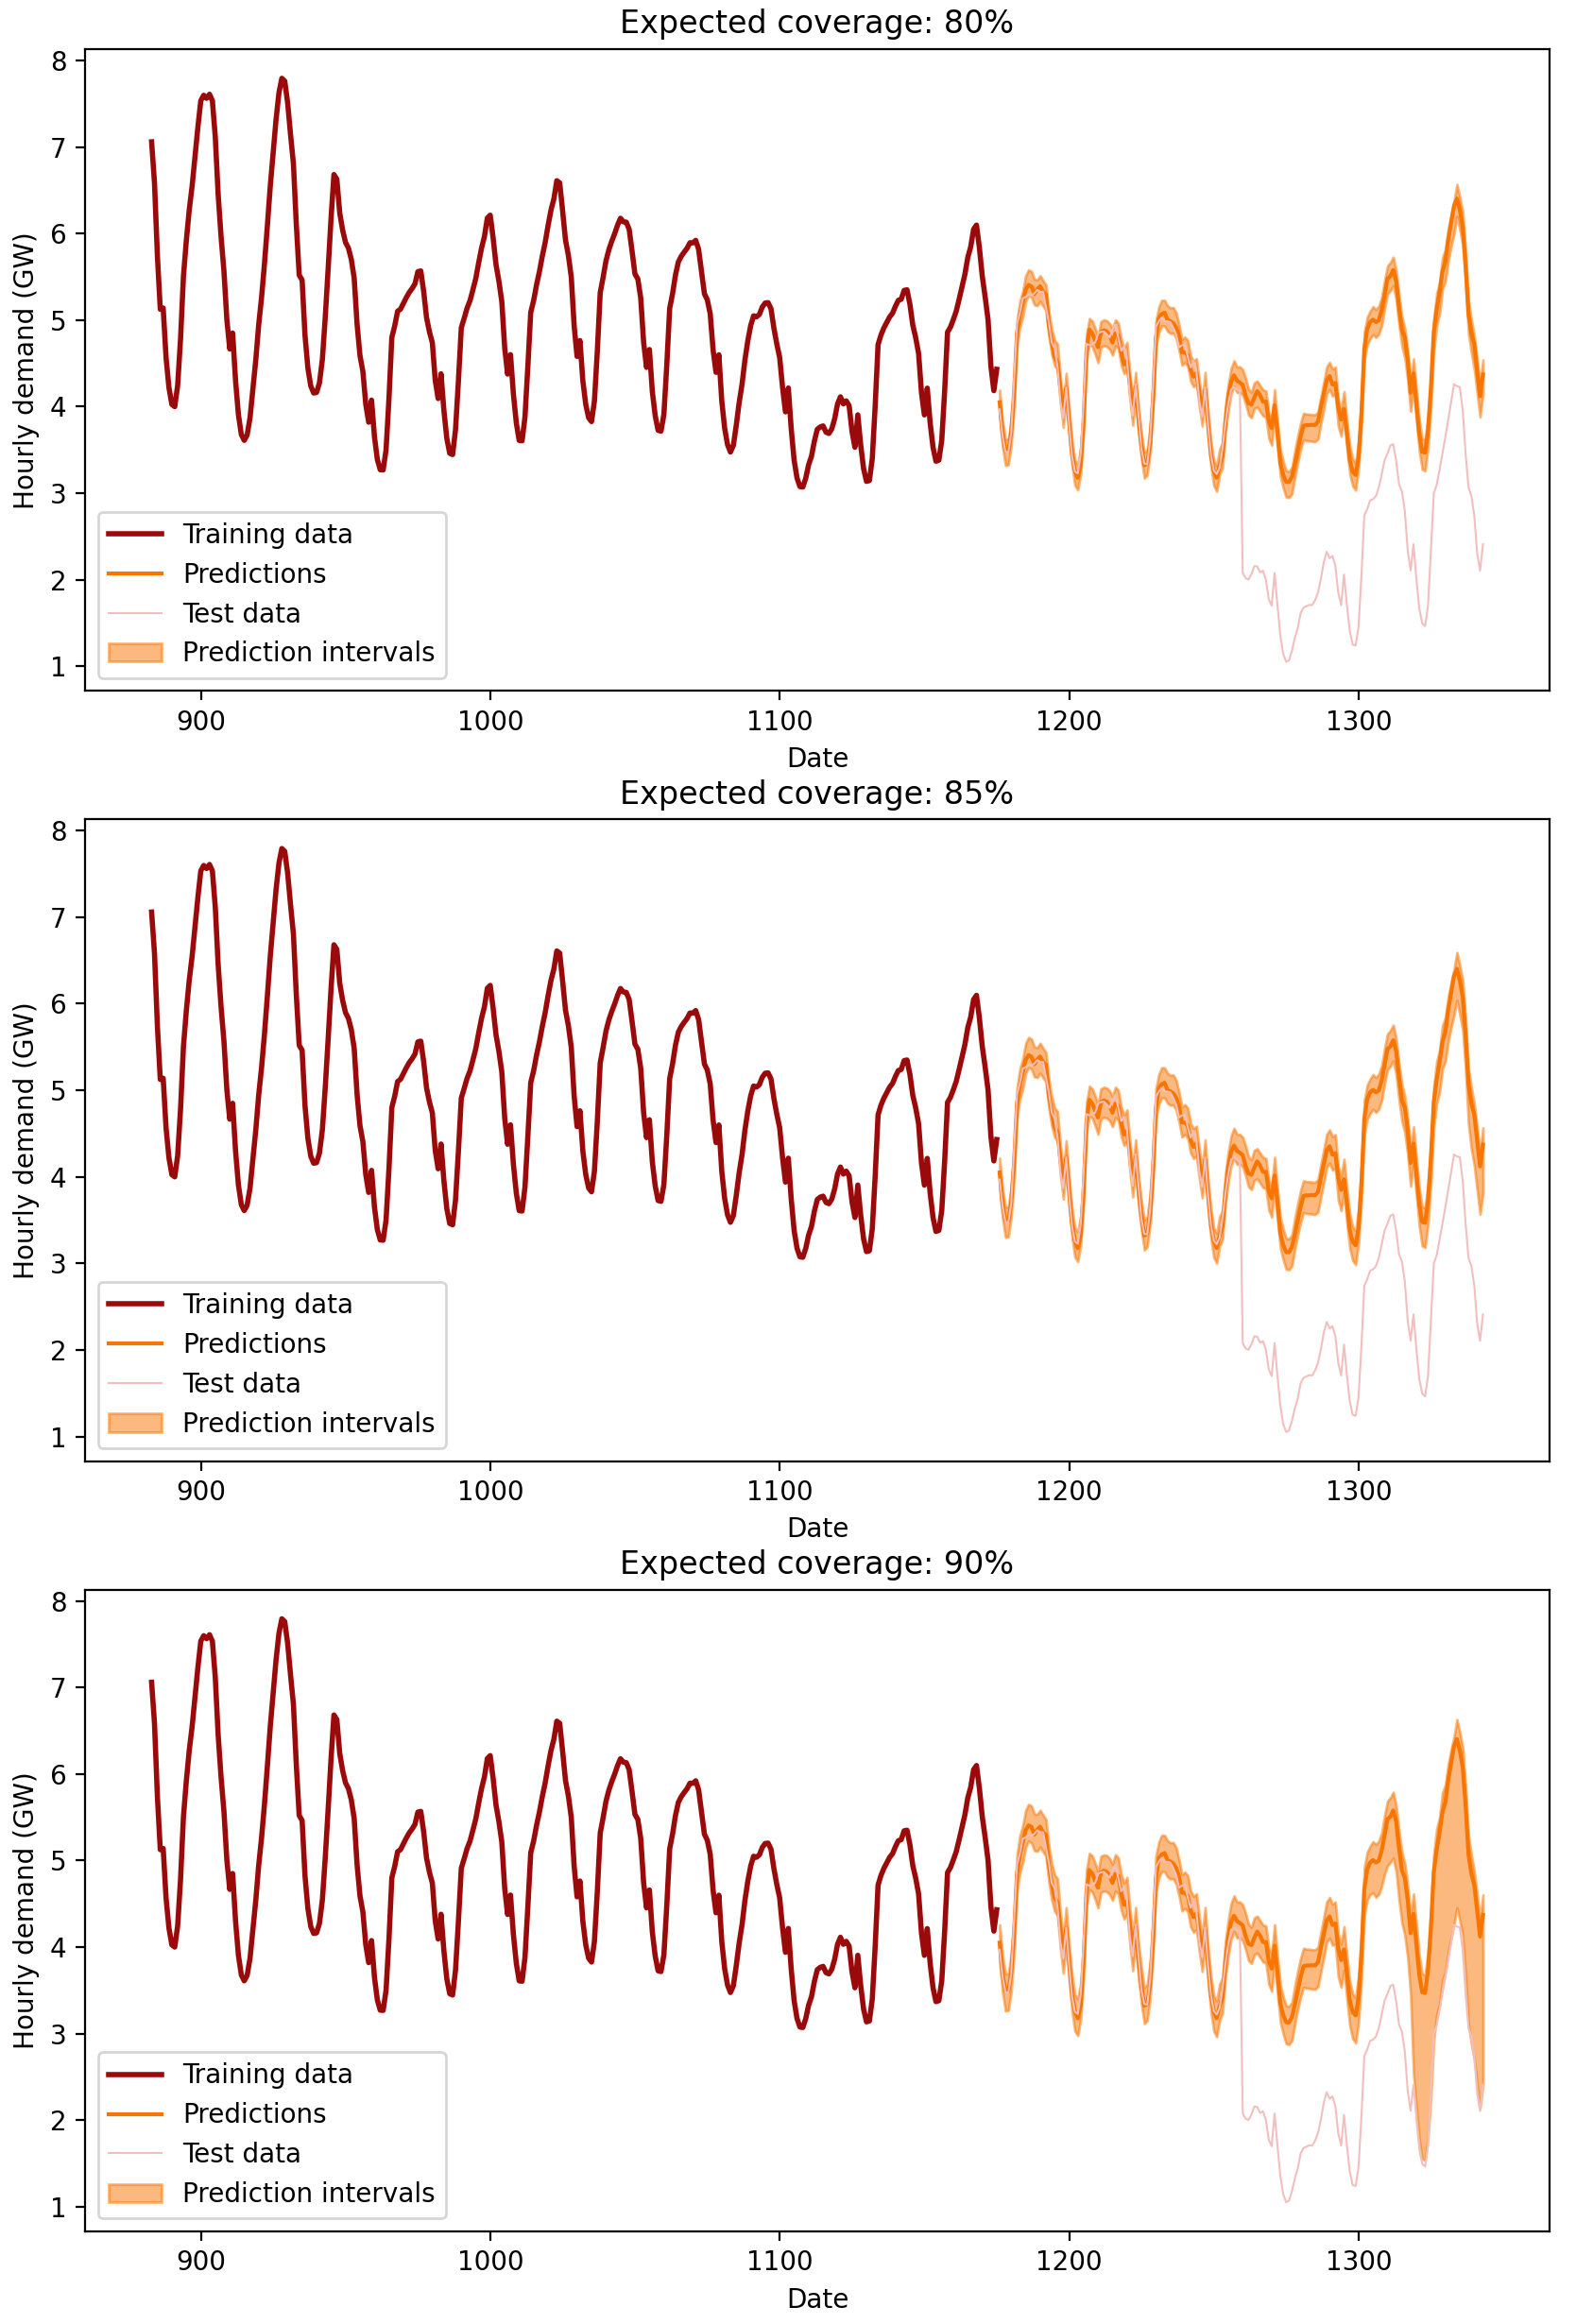
\includegraphics[width=\textwidth, height=1.25\textwidth]{Figures/timeseries/with-change-point/prediction-intervals-in-function-of-miscoverage.png}
    \caption{EnbPI with partial fit recovering intervals' width at different pace, for different $\a$ values (from top to bottom: $\a=0.20, 0.15, 0.10$).}
    \label{fig:timeseries-intervals-alpha-cpoint}
\end{figure}

These different speeds can also be noted at sub-figure \ref{subfig:timeseries-coverage-alpha-cpoint}, in which the attained global coverage for the EnbPI strategy varies non-linearly with $\a$.\\  

\begin{figure}[ht]
    \centering
    %\hspace{-10mm}
    \begin{subfigure}[b]{0.32\textwidth}
        \centering
        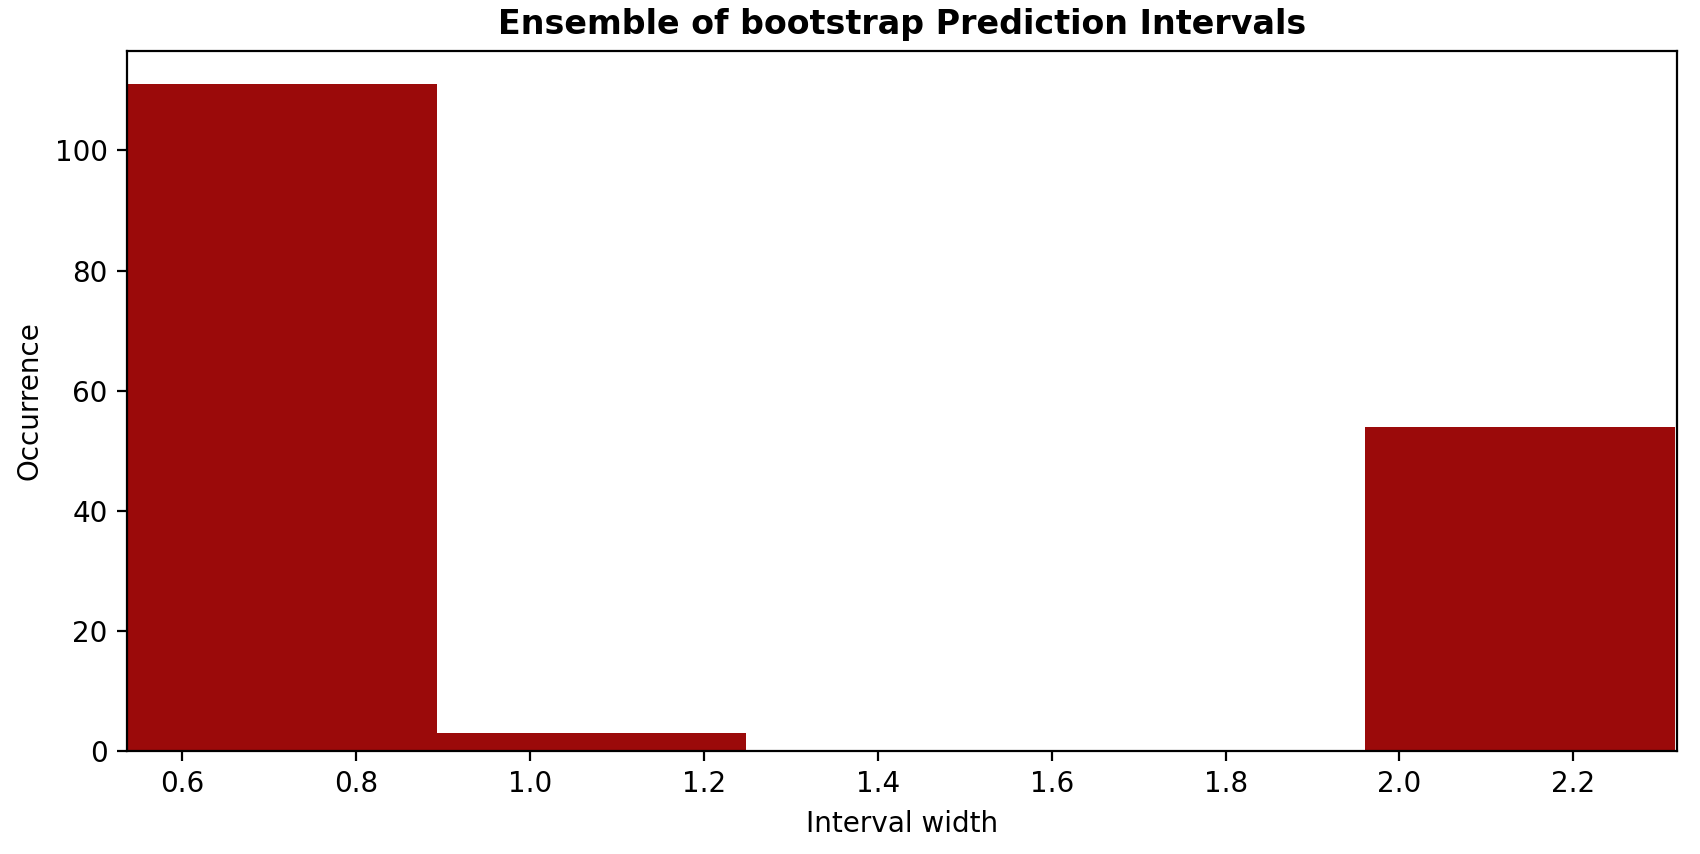
\includegraphics[width=1.05\textwidth, height=0.85\textwidth]{Figures/timeseries/with-change-point/width-occurrence-timeseries-problem-with-change-point.png}
        \caption{Intervals' width histograms}
        \label{subfig:timeseries-width-histograms-cpoint}
    \end{subfigure}
    \hfill
    \begin{subfigure}[b]{0.32\textwidth}
        \centering
        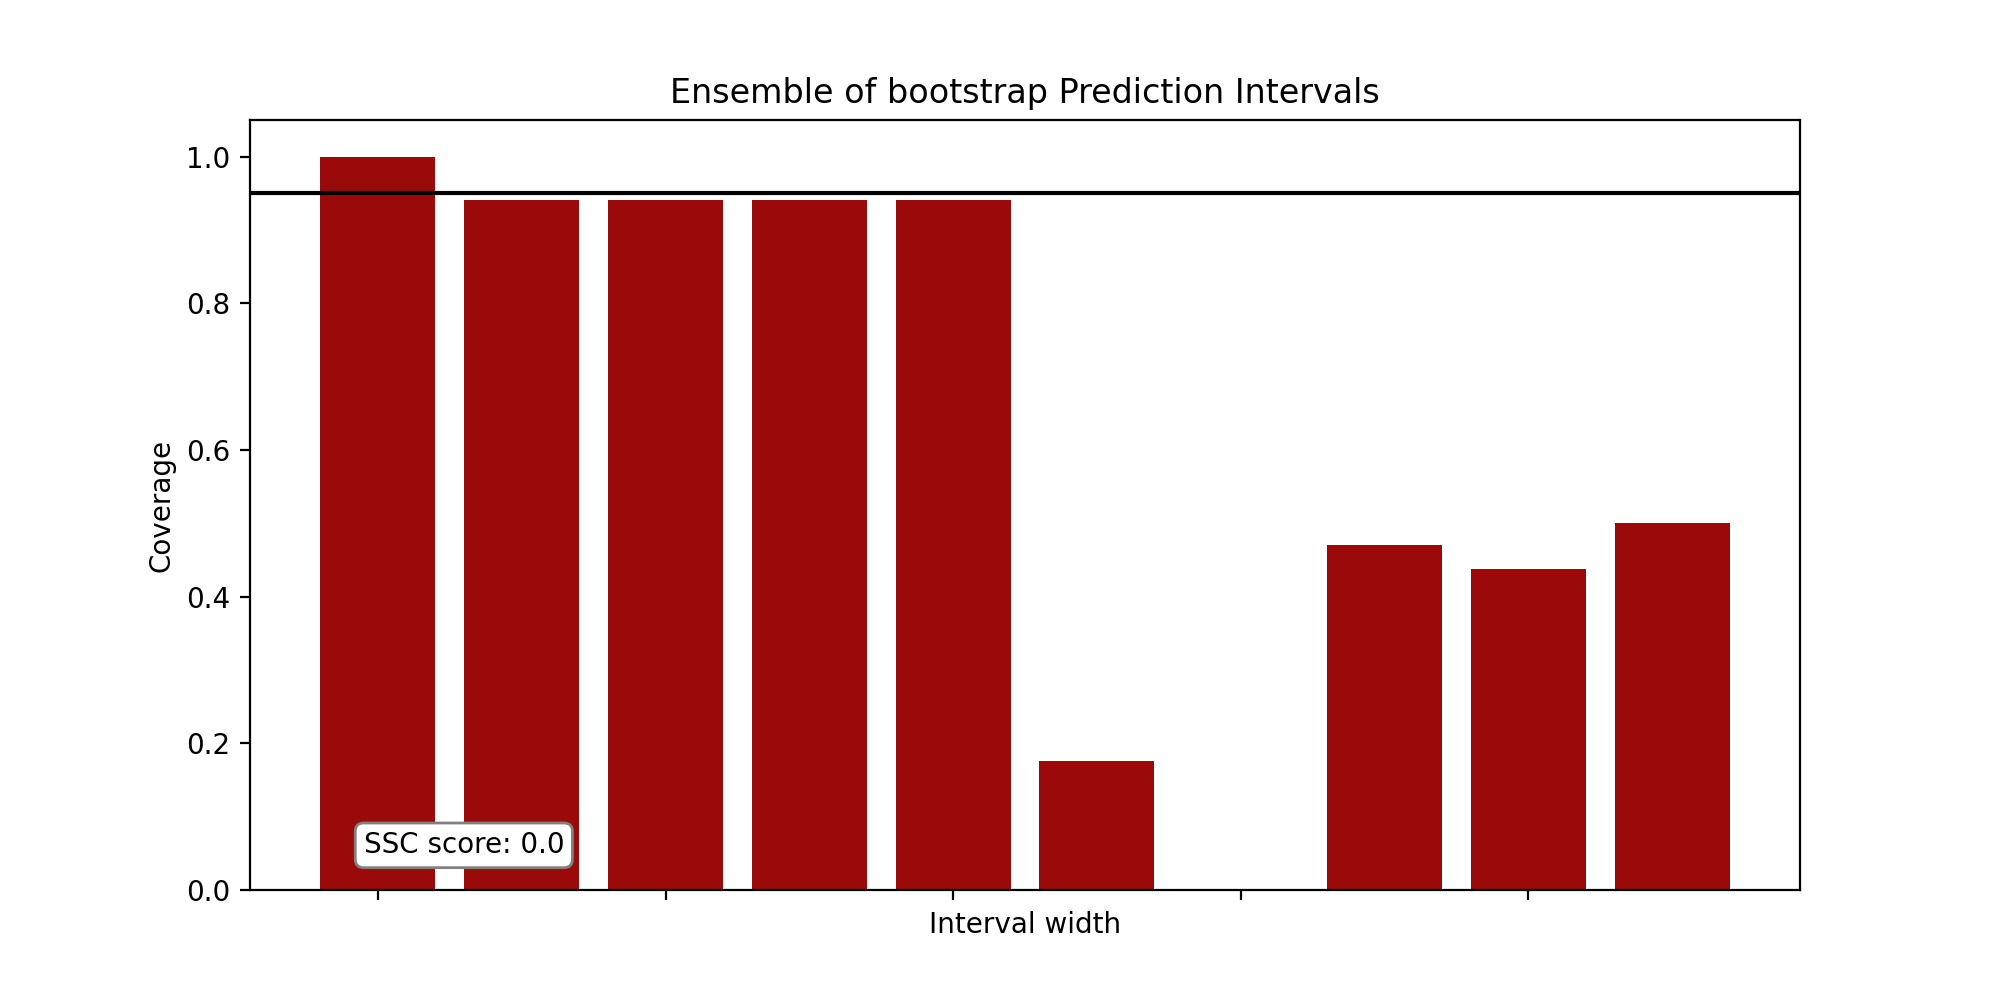
\includegraphics[width=1.15\textwidth, height=0.85\textwidth]{Figures/timeseries/with-change-point/coverage-vs-width-timeseries-problem-with-change-point.png}
        \caption{Coverage in function of intervals' width}
        \label{subfig:timeseries-coverage-width-cpoint}
    \end{subfigure}
    \hfill % adds horizontal space between figures
    \begin{subfigure}[b]{0.32\textwidth} % Adjust the width to fit your needs
        \centering
        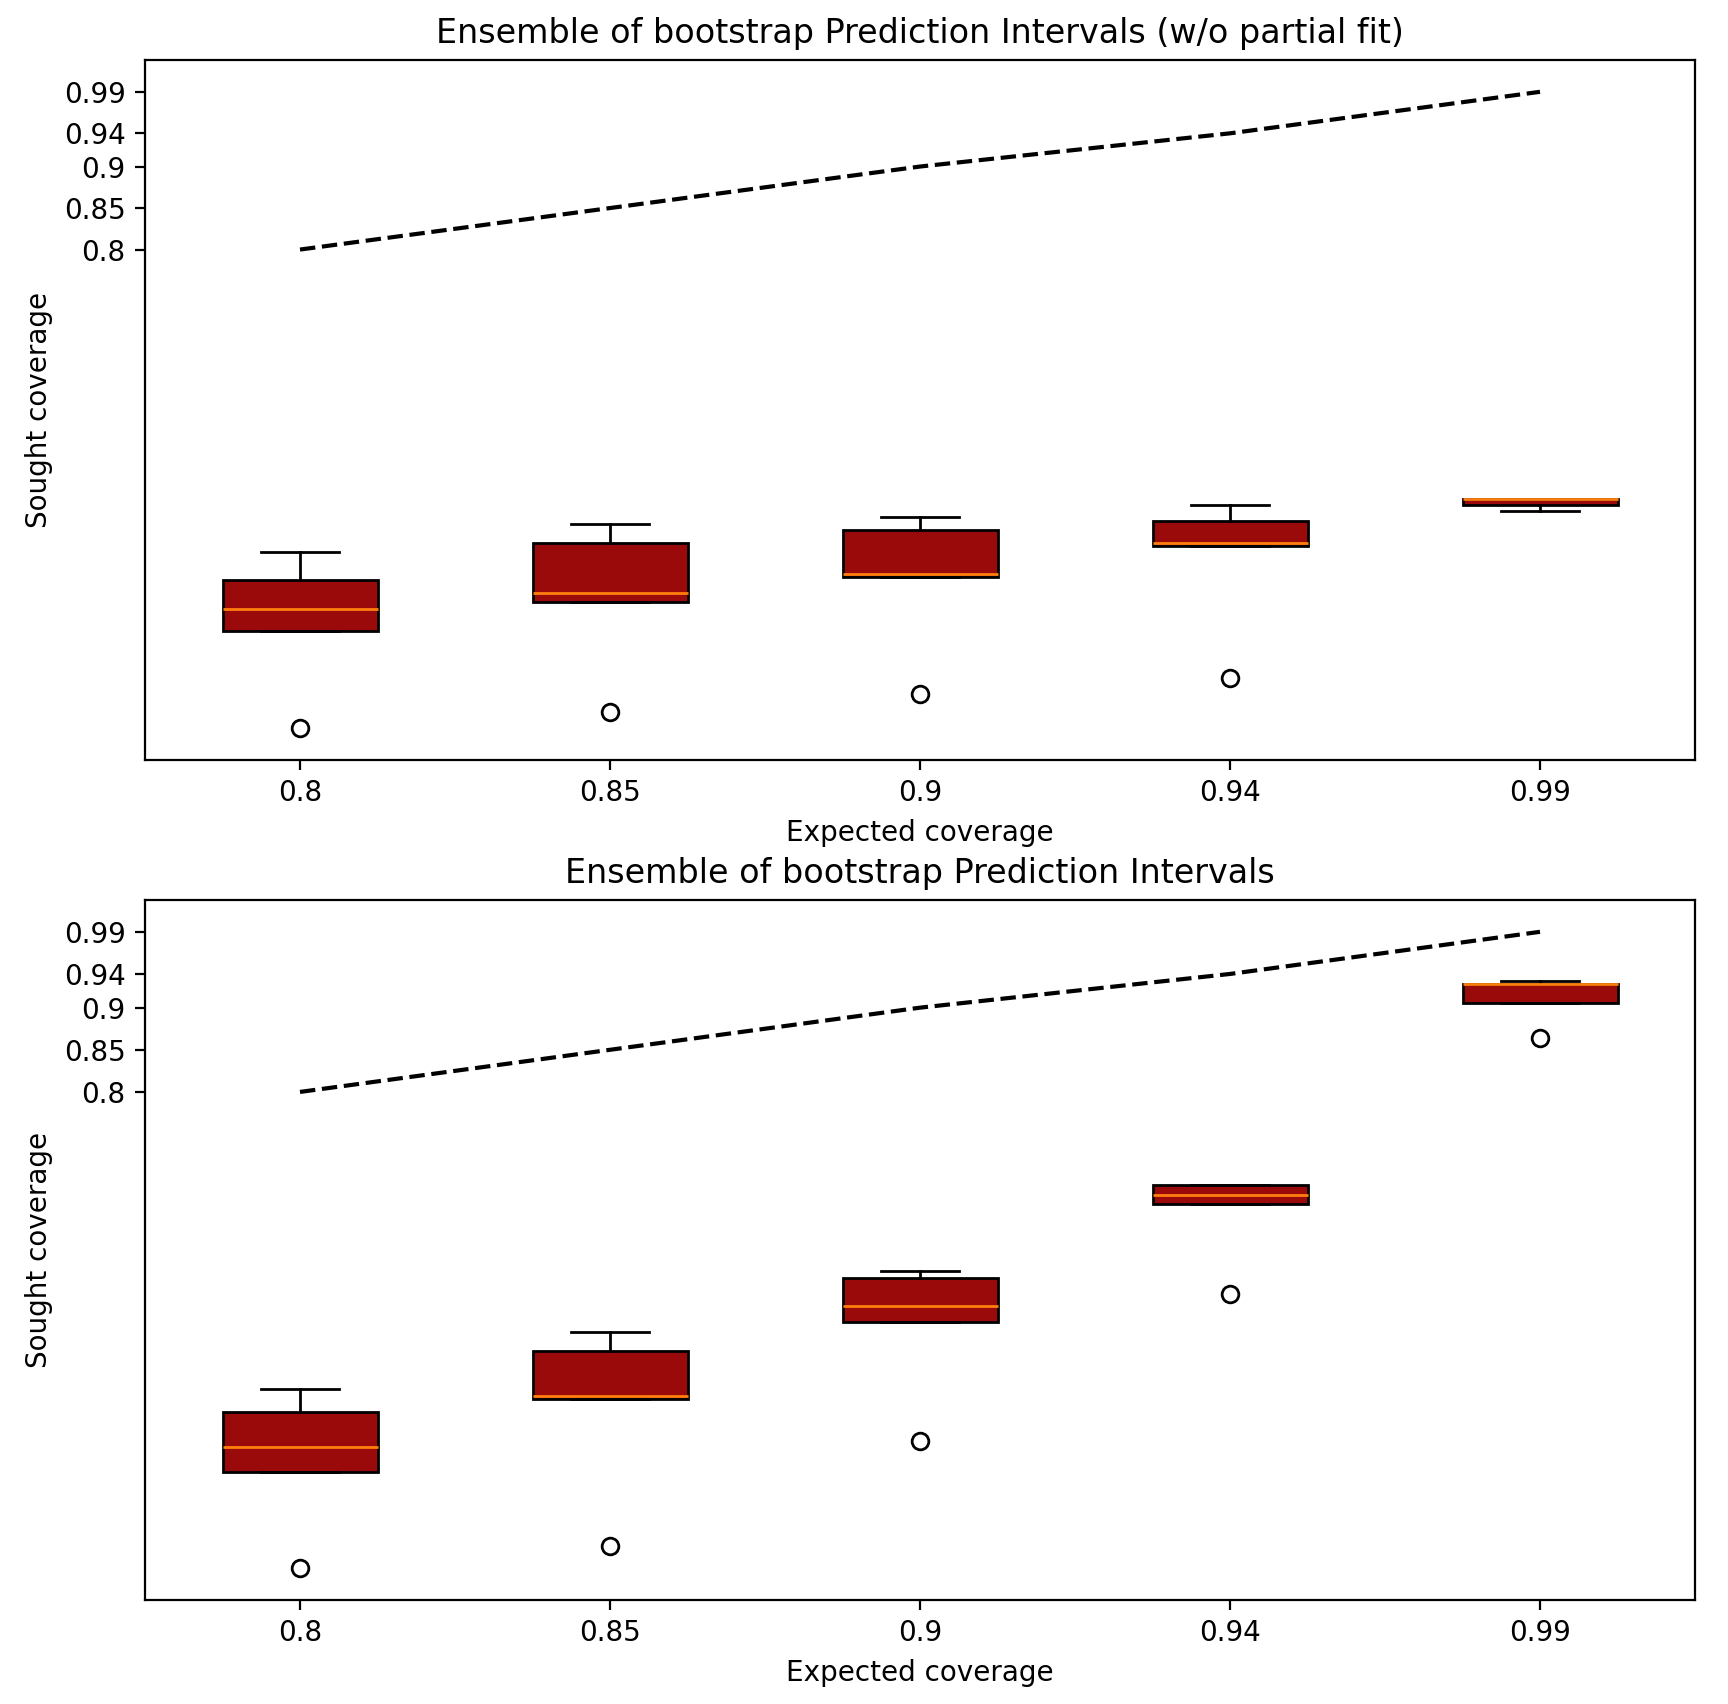
\includegraphics[width=1.15\textwidth, height=1.75\textwidth]{Figures/timeseries/with-change-point/coverage-vs-alpha-timeseries-problem-with-change-problem.png} % Adjust the filename and path
        \caption{Coverage in function of $\a$}
        \label{subfig:timeseries-coverage-alpha-cpoint}
    \end{subfigure}
    \caption{Width \& coverage distributions for the change point's (test) data ($\a=0.05$) for EnbPI. At subfigure \ref{subfig:timeseries-coverage-alpha-cpoint}, EnbPI\_{}nP \& EnbPI are displayed (top \& bottom, respectively).}
    \label{fig:timeseries-width-coverage-cpoint}
\end{figure}

Finally, while in sub-figures \ref{subfig:timeseries-width-histograms-cpoint} \& \ref{subfig:timeseries-coverage-width-cpoint} the adaptive feature of EnbPI intervals\footnote{Note the change point is also perceived with these 2 visualizations: the widest intervals correspond to those with less conditional coverage, since those were issued after the change point's recovery.} is shown; in Figure \ref{fig:timeseries-rolling-coverage-cpoint} the EnbPI's progressive coverage recovery is featured in function of time with a rolling window (while indeed EnbPI\_{}nP does not recover at all).

\begin{figure}[ht]
    \centering
    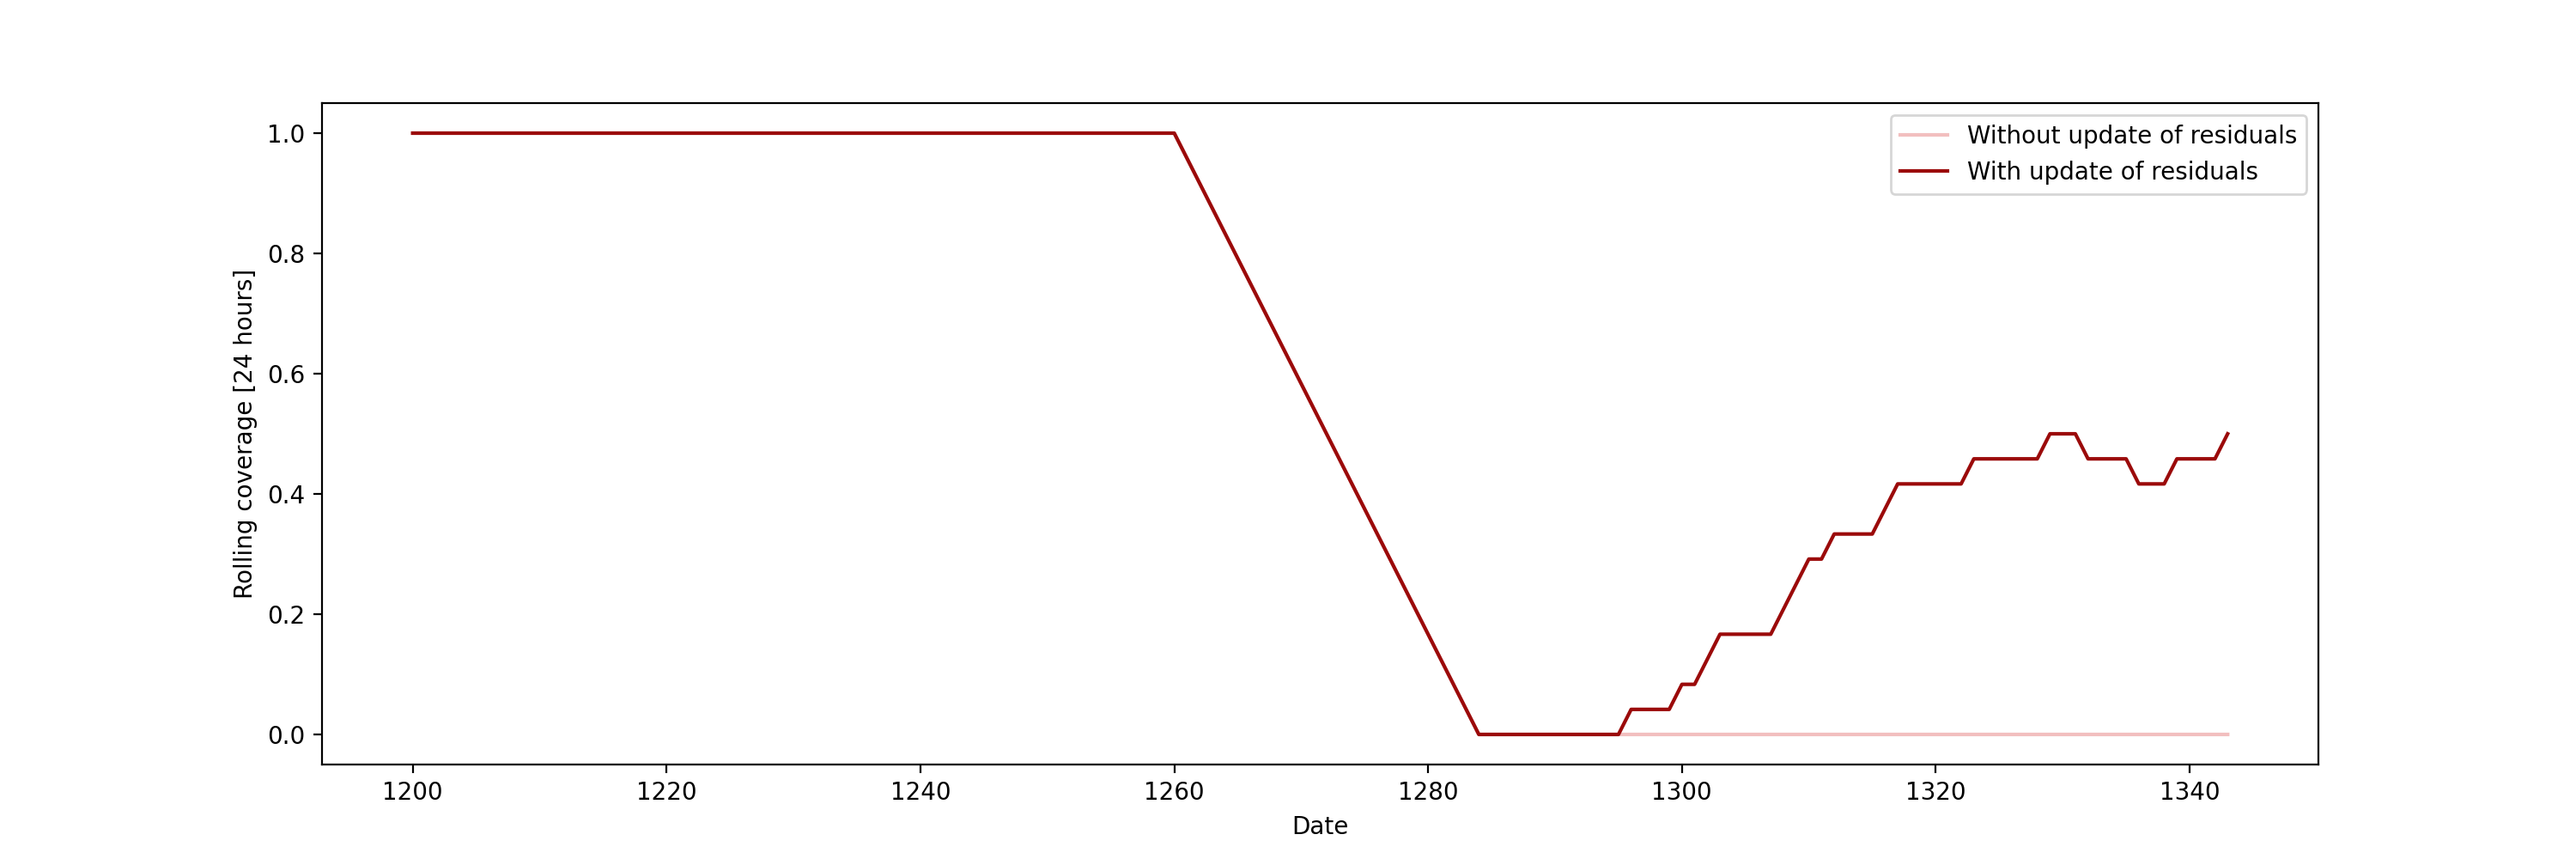
\includegraphics[width=\textwidth]{Figures/timeseries/with-change-point/rolling-coverage-with-change-point.png}
    \caption{Coverage in function of time (grouped within 24h rolling windows) for the EnbPI strategies (and change point's data).}
    \label{fig:timeseries-rolling-coverage-cpoint}
\end{figure}
\chapter{Conclusions}\label{chap:conclusions}

Throughout this work, several methods have been theoretically justified and successfully applied to quantify the prediction uncertainty both for regression and time series problem. These strategies are distribution-free \& model-agnostic and stem from the notion of "\textit{conformalizing}" predictions to data and using the residuals to understand the errors distribution. That is why they are grouped within the so-called "conformal prediction" (CP) methodologies.\\

Even though CP paradigm was classically applied only under "\textit{data exchangeability}" conditions, this work has reviewed some of the most recent \& non-trivial efforts to enable CP when this hypothesis is not fulfilled. 

In particular, while SCP, CV$+$, J$+$aB \& CQR were studied for the exchangeable case; regarding the time series case, "\textit{EnbPI}" (\cite{chenxu2021a}) was presented as the strategy to effectively obtain prediction intervals with statistically valid coverage.

While all the former strategies were successfully applied to practical case, generally providing valid intervals, below the more fine-grained conclusions are listed:
\begin{itemize}
    \item \textbf{Exchangeable case} (regression problem):
    \begin{itemize}
        \item The best strategies, \textbf{decreasingly ordered} by:
        \begin{itemize}
            \item \textit{Statistical efficiency} are: CQR, SCP, CV$+$, J$+$aB. This is fulfilled independently of $\a$.
            \item \textit{Computational efficiency} are: SCP, CQR, CV$+$, J$+$aB.
            \item \textit{Predictive power} are: CV$+$ \& J$+$aB, SCP, CQR.
            \item "\textit{Informativeness}" (coverage-width ratio) are: J$+$aB, SCP, CQR, CV$+$.
            \item \textit{Adaptability} are: CQR, CV$+$, J$+$aB (slight to none). Contrarily, SCP intervals are not adaptive at all. 
        \end{itemize}
        \item \textbf{CQR} seems the best \textbf{strategy} to achieve the best \textbf{marginal} \& \textbf{conditional coverage}, when dataset is large enough. 

        Thus, it may result suitable when a conservative and statistical efficient tool is needed.
        \item \textbf{J$+$aB} seems the best \textbf{strategy} to achieve the best \textbf{informative intervals} (maximizing predictive power, while minimizing intervals width), at expenses of no-adaptability \& losing some coverage. 
        
        Thus, it may result suitable when more reckless guesses can be afforded and low training \& inference times are not a requirement.
    \end{itemize}
    \item \textbf{Non-exchangeable case} (time series problem):
    \begin{itemize}
        \item \textbf{EnbPI} is a \textbf{suitable option} to provide valid intervals for \textbf{time series problems}.
        \item In general, and particularly when there might be strong shifts in data, EnbPI's intervals adjustment using test residuals (its "partial fit" feature) is of crucial importance.
        \item This "\textbf{partial fit}" option will not only allow the intervals' coverage \textbf{recover from change points}, but also will allow all the issued \textbf{intervals} to be \textbf{adaptive}.
    \end{itemize}
\end{itemize} 

\section{Further research}\label{sec:further-research}

There a huge number of relevant other inquiries and research lines which could extend this work, but were out of the scope of this thesis. 
Below, some of them are reviewed: 
\begin{itemize}
\item Leverage cross-validation folds in the CQR strategy, instead of a simple train-test split of the dataset, to improve the predictive power and reduce the need of a large dataset. 
\item Implement other contemporary CP methodologies for time series problems, such as \textit{Adaptive Conformal Inference}, ACI (\cite{gibbs2021}) and the more recent \textit{Hopfield Conformal Prediction Trees}, HopCPT (\cite{auer2023}); in order to compare performance differences and their suitability.
\item Extend all these methods to the multi-dimensional output variables' case, to broaden their applicability to multi-output regression \& time series problems.
\item Apply the former methodologies to classification problems (discrete target variables) and discuss whether similar conclusions to their continuous counter-part can be drawn.
\end{itemize}

%----------------------------------------------------------------------------------------
%	THESIS CONTENT - APPENDICES
%----------------------------------------------------------------------------------------

\appendix % Cue to tell LaTeX that the following "chapters" are Appendices
\chapter{Regression problem}
\label{app:regression-problem} 

Unless it is specified otherwise, the miscoverage level was set to $\a=0.2$ (\textit{i.e.} $80\%$ of expected coverage) for the visualizations.

\begin{figure}[ht]
    \centering
    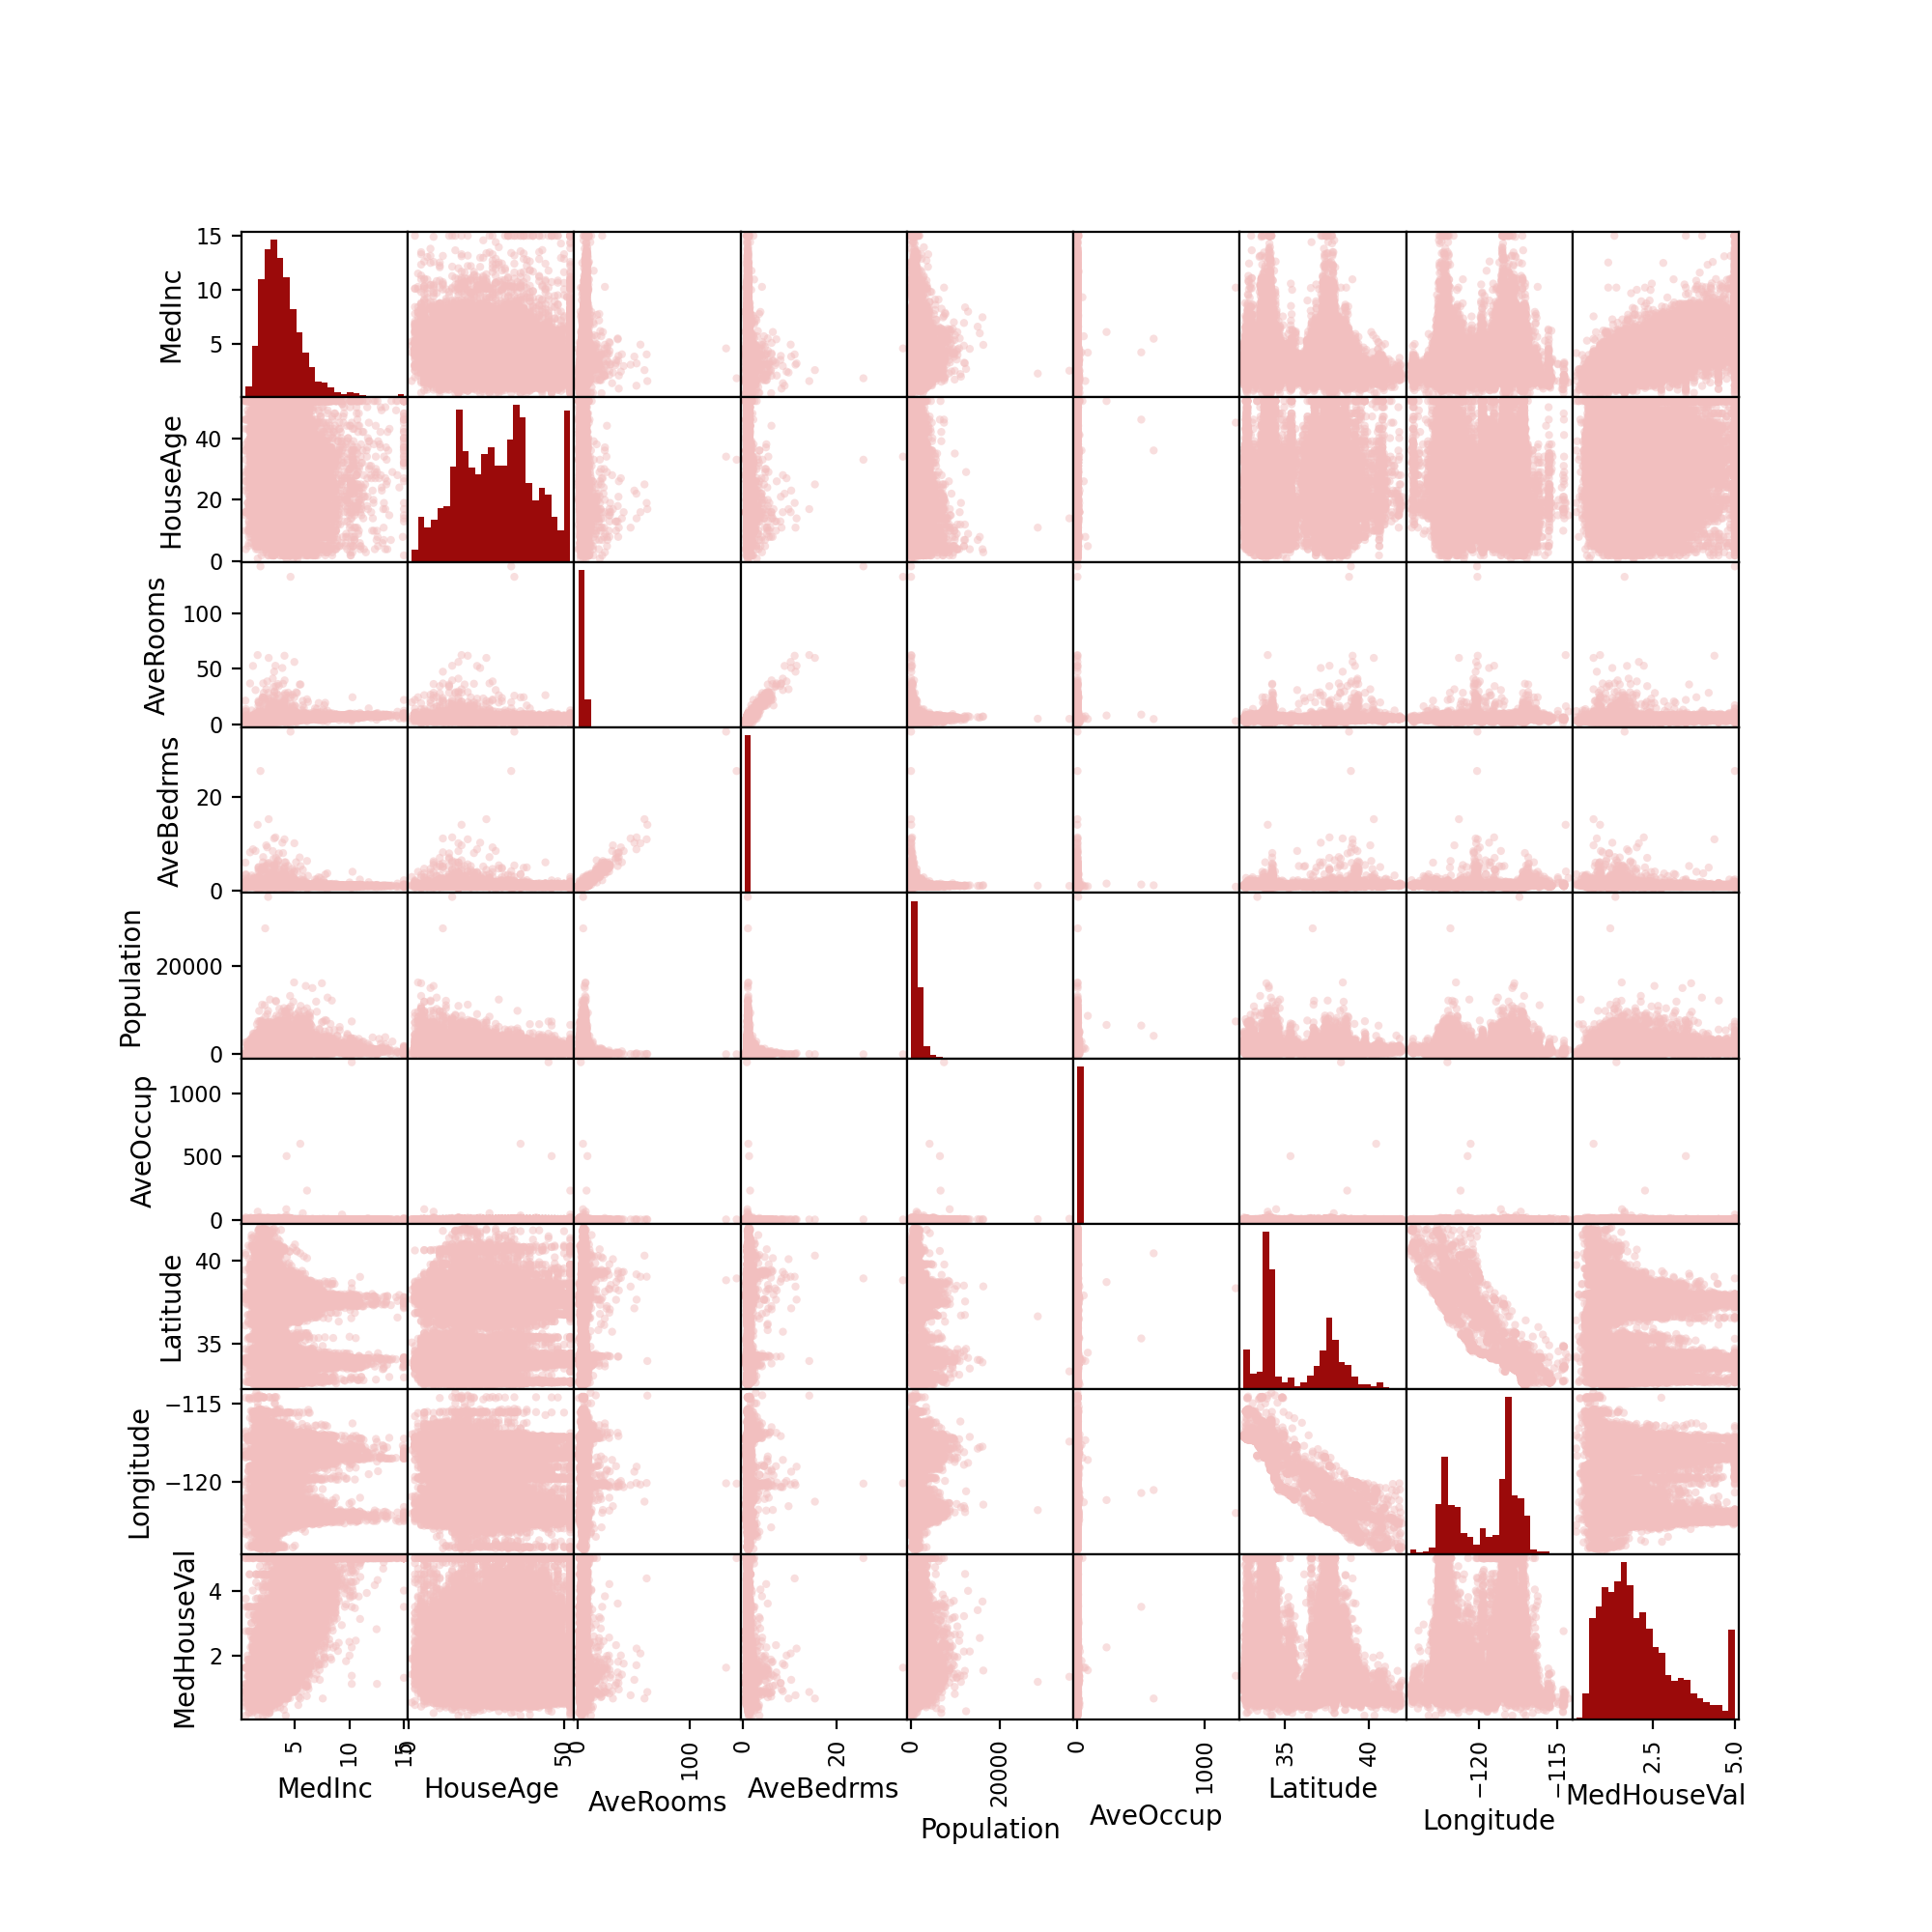
\includegraphics[width=0.8\textwidth]{Figures/regression/data-regression-problem.png}
    \caption{Marginal distributions for each of the possible combinations of the regression problem's features.}
    \label{fig:app-regression-data-distribution}
\end{figure}

\begin{figure}[ht]
    \centering
    \hspace{-10mm}
    \begin{subfigure}[b]{0.48\textwidth}
        \centering
        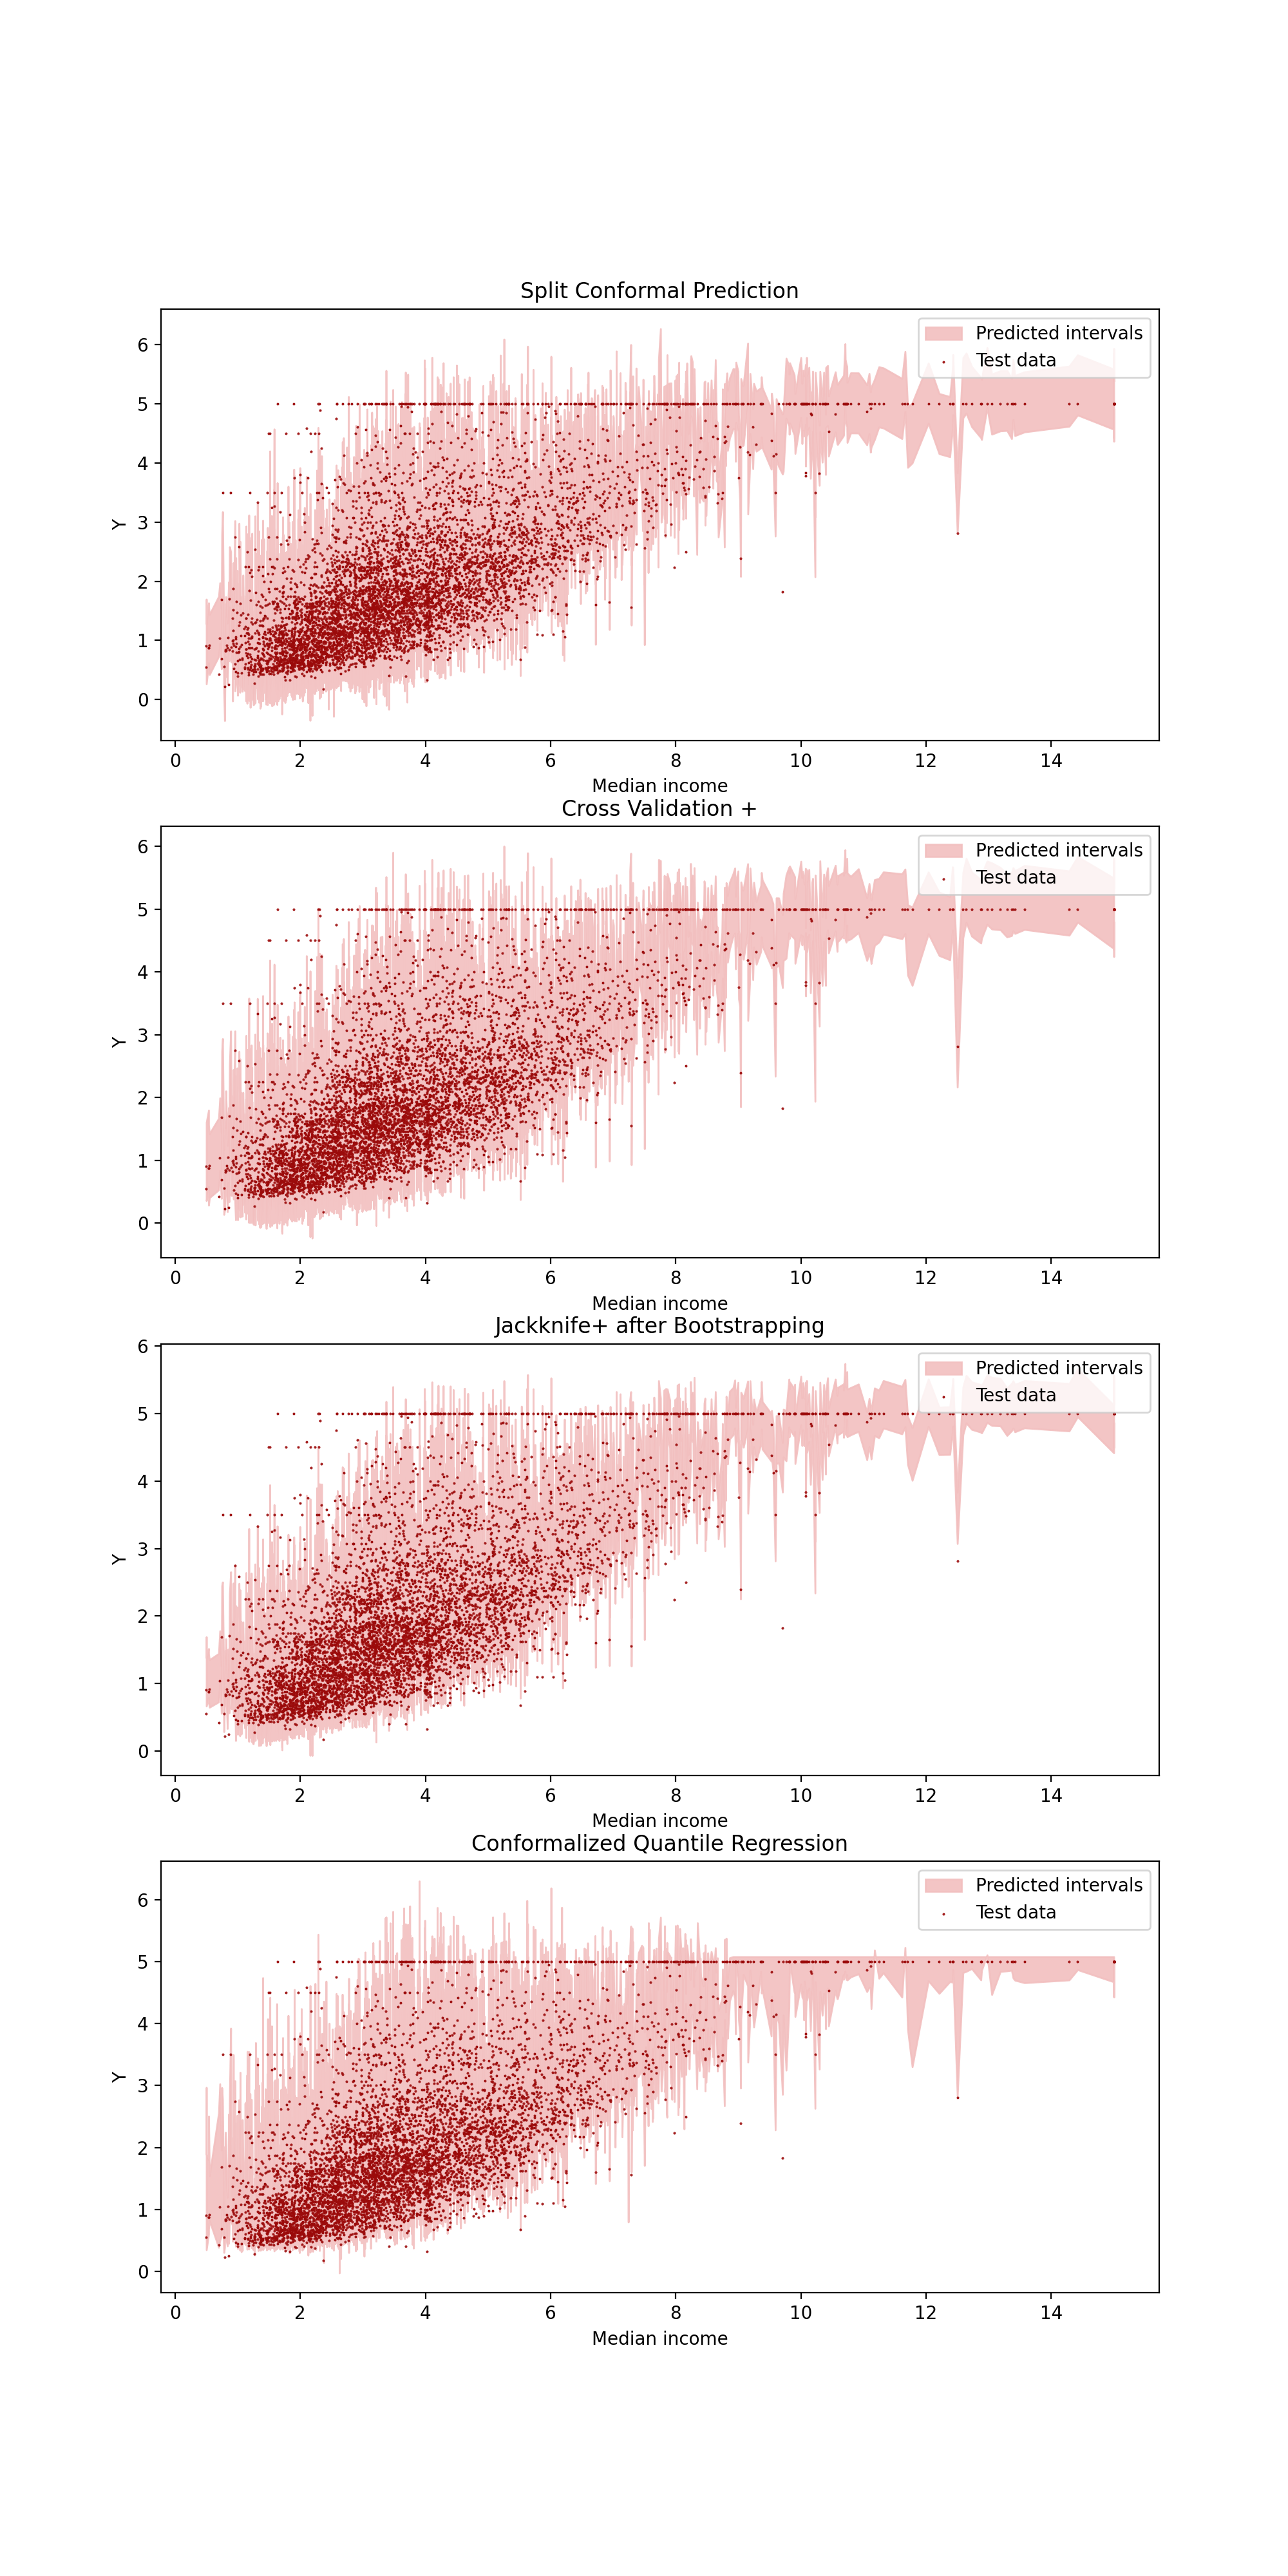
\includegraphics[width=1.2\textwidth, height=3.35\textwidth]{Figures/regression/prediction-intervals-regression-problem.png}
        \caption{Prediction intervals}
        \label{subfig:app-regression-prediction-intervals}
    \end{subfigure}
    \hfill % adds horizontal space between figures
    \begin{subfigure}[b]{0.48\textwidth} % Adjust the width to fit your needs
        \centering
        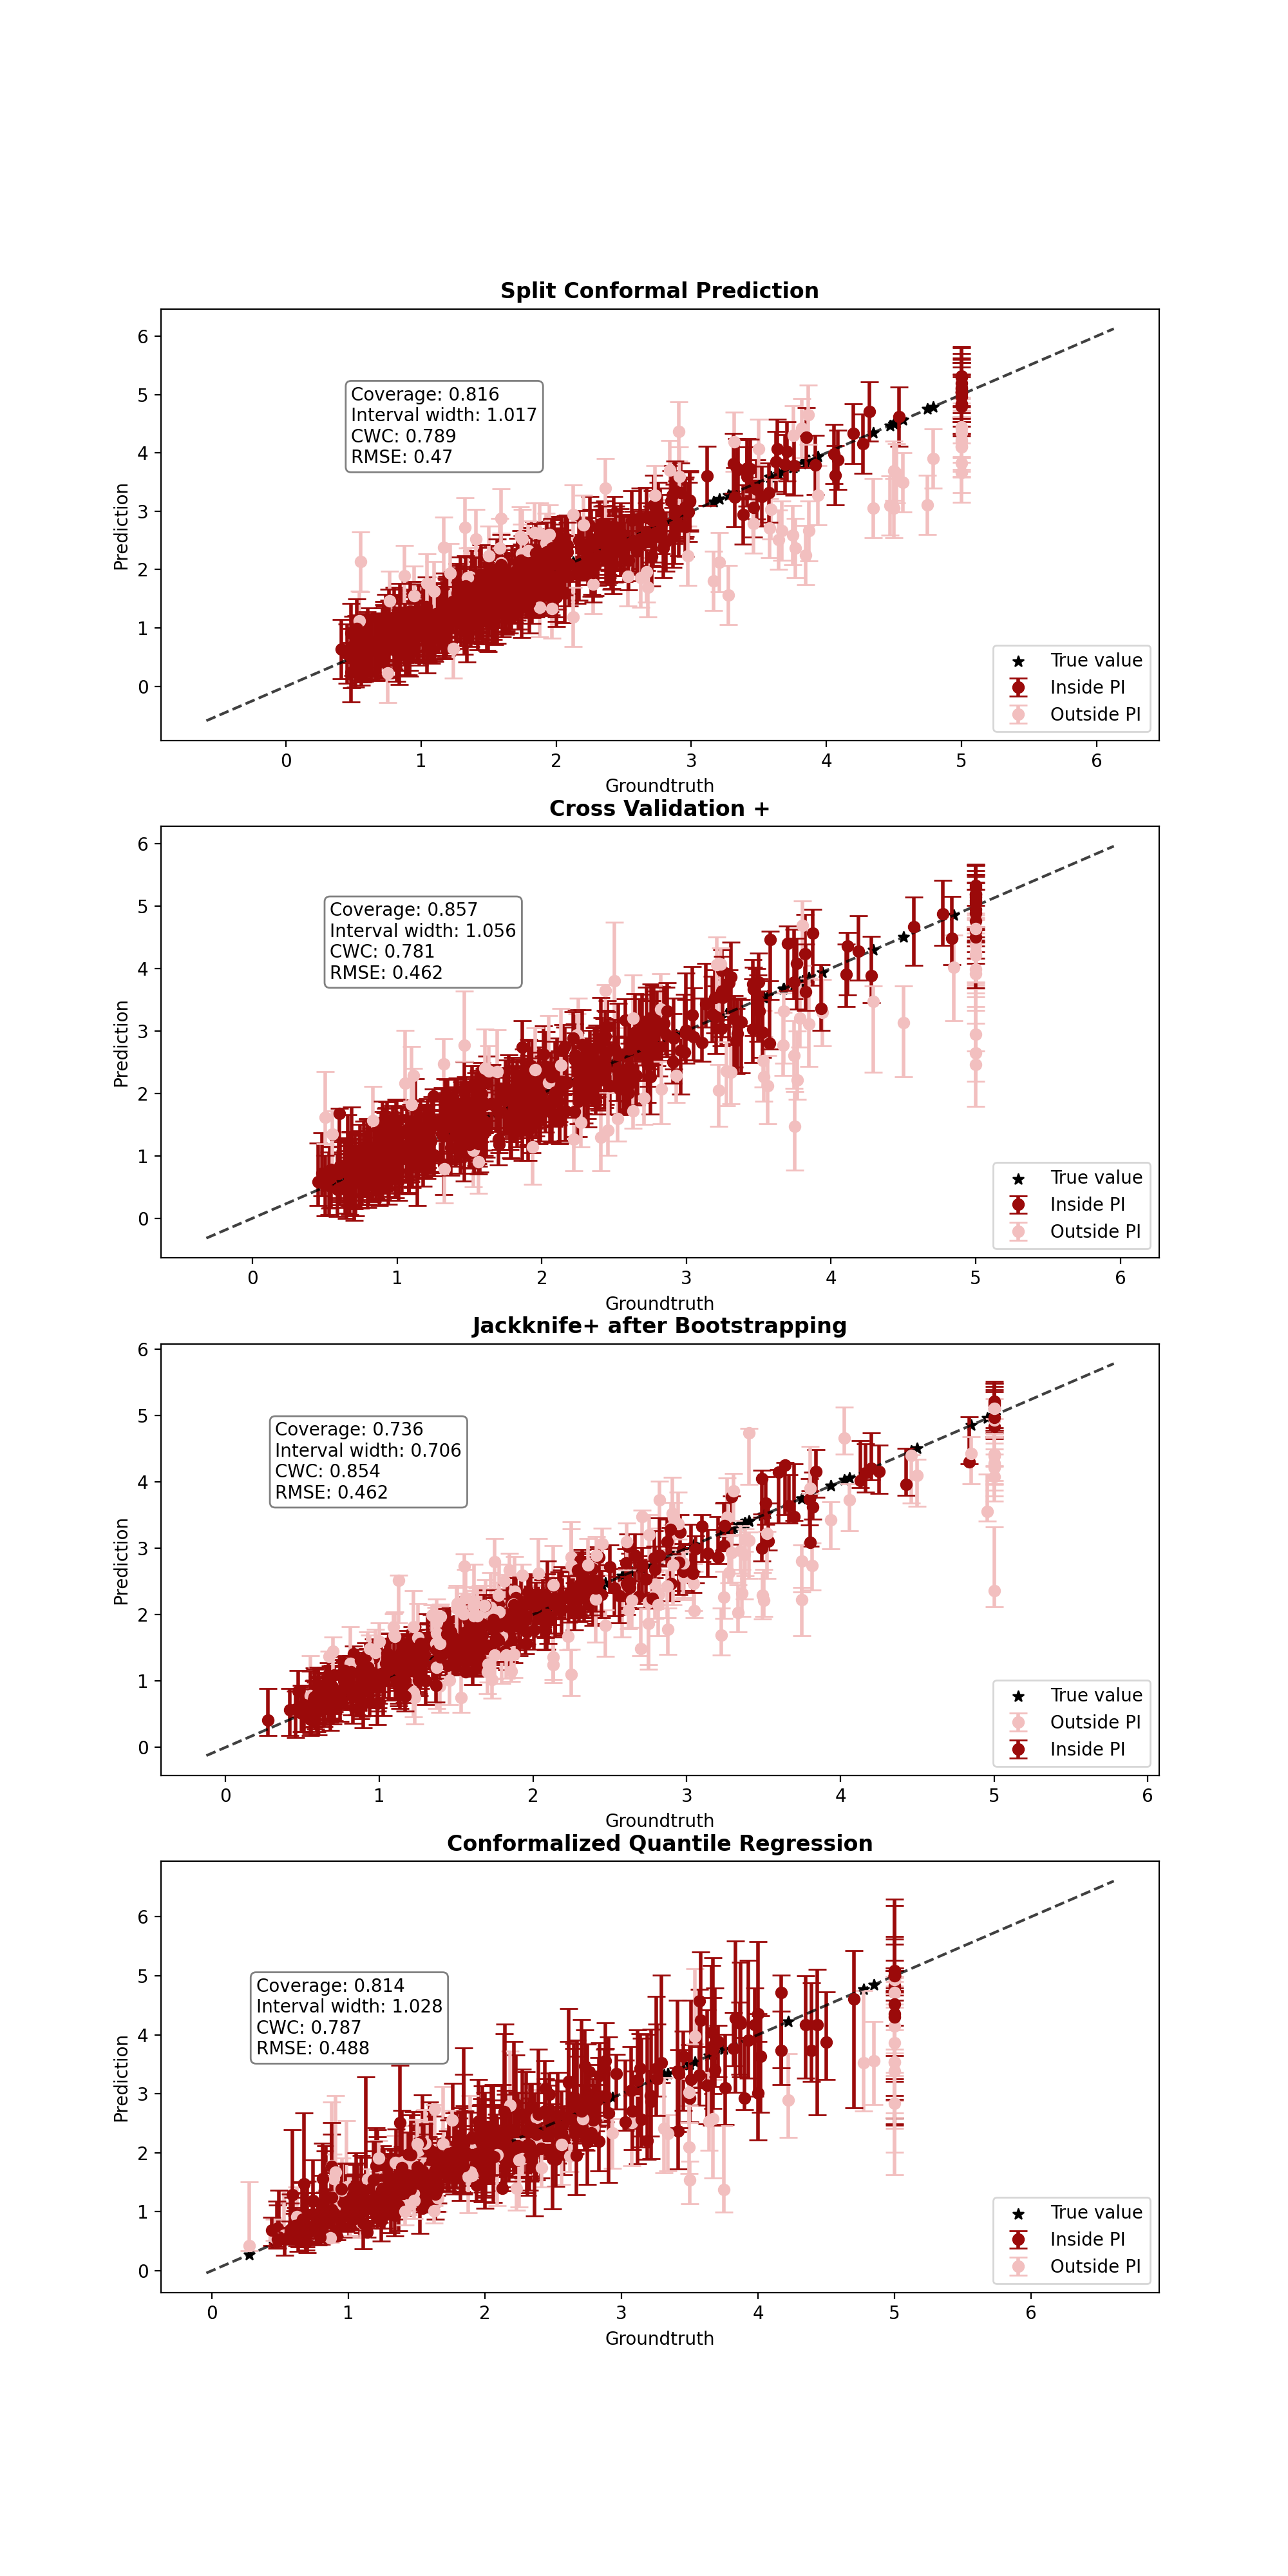
\includegraphics[width=1.2\textwidth, height=3.35\textwidth]{Figures/regression/average-goodness-regression-problem.png} % Adjust the filename and path
        \caption{Goodness of the prediction intervals (prediction vs. ground truth). Just $7.5\%$ was used for visualization purposes.}
        \label{subfig:app-regression-intervals-goodness}
    \end{subfigure}
    \caption{Visualizations related to the prediction intervals for the test data and 4 different strategies, from top to bottom: SCP, CV$+$, J$+$aB and CQR.}
    \label{fig:app-regression-intervals}
\end{figure}

\begin{figure}[ht]
    \centering
    %\hspace{-10mm}
    \begin{subfigure}[b]{0.32\textwidth}
        \centering
        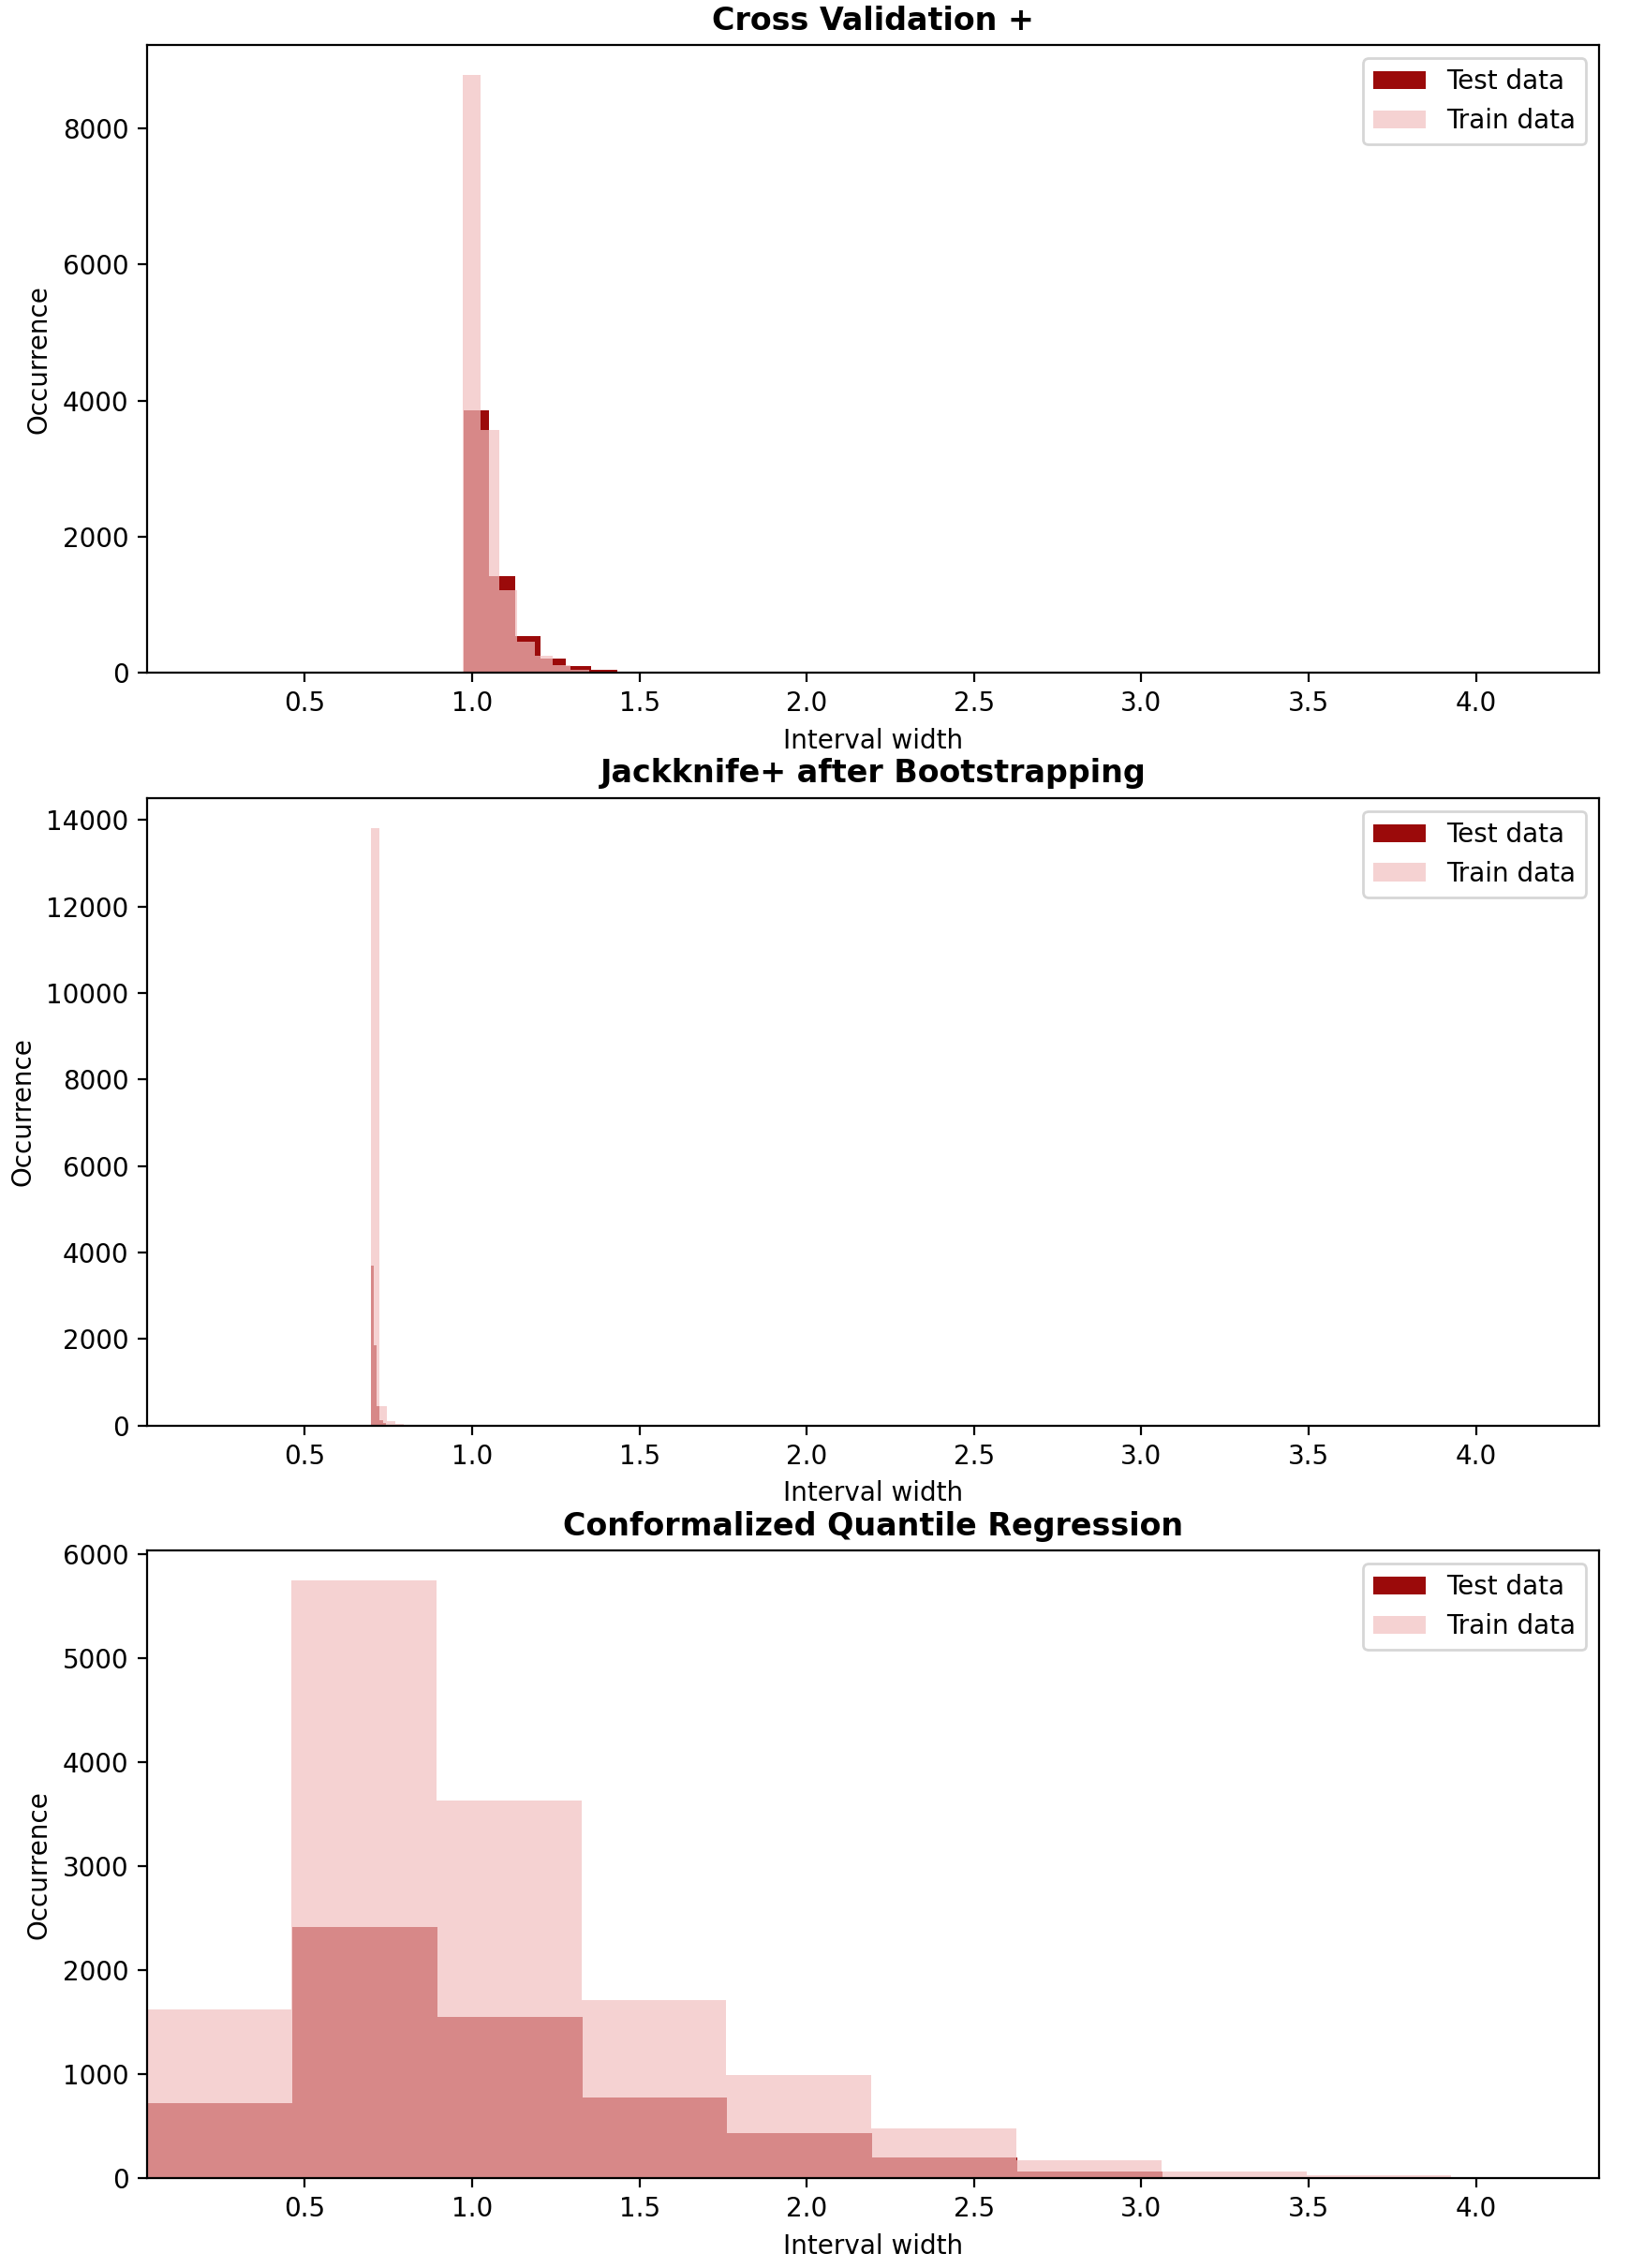
\includegraphics[width=1.15\textwidth, height=3.05\textwidth]{Figures/regression/width-occurrence-regression-problem.png}
        \caption{Intervals' width histograms}
        \label{subfig:app-regression-width-histograms}
    \end{subfigure}
    \hfill
    \begin{subfigure}[b]{0.32\textwidth}
        \centering
        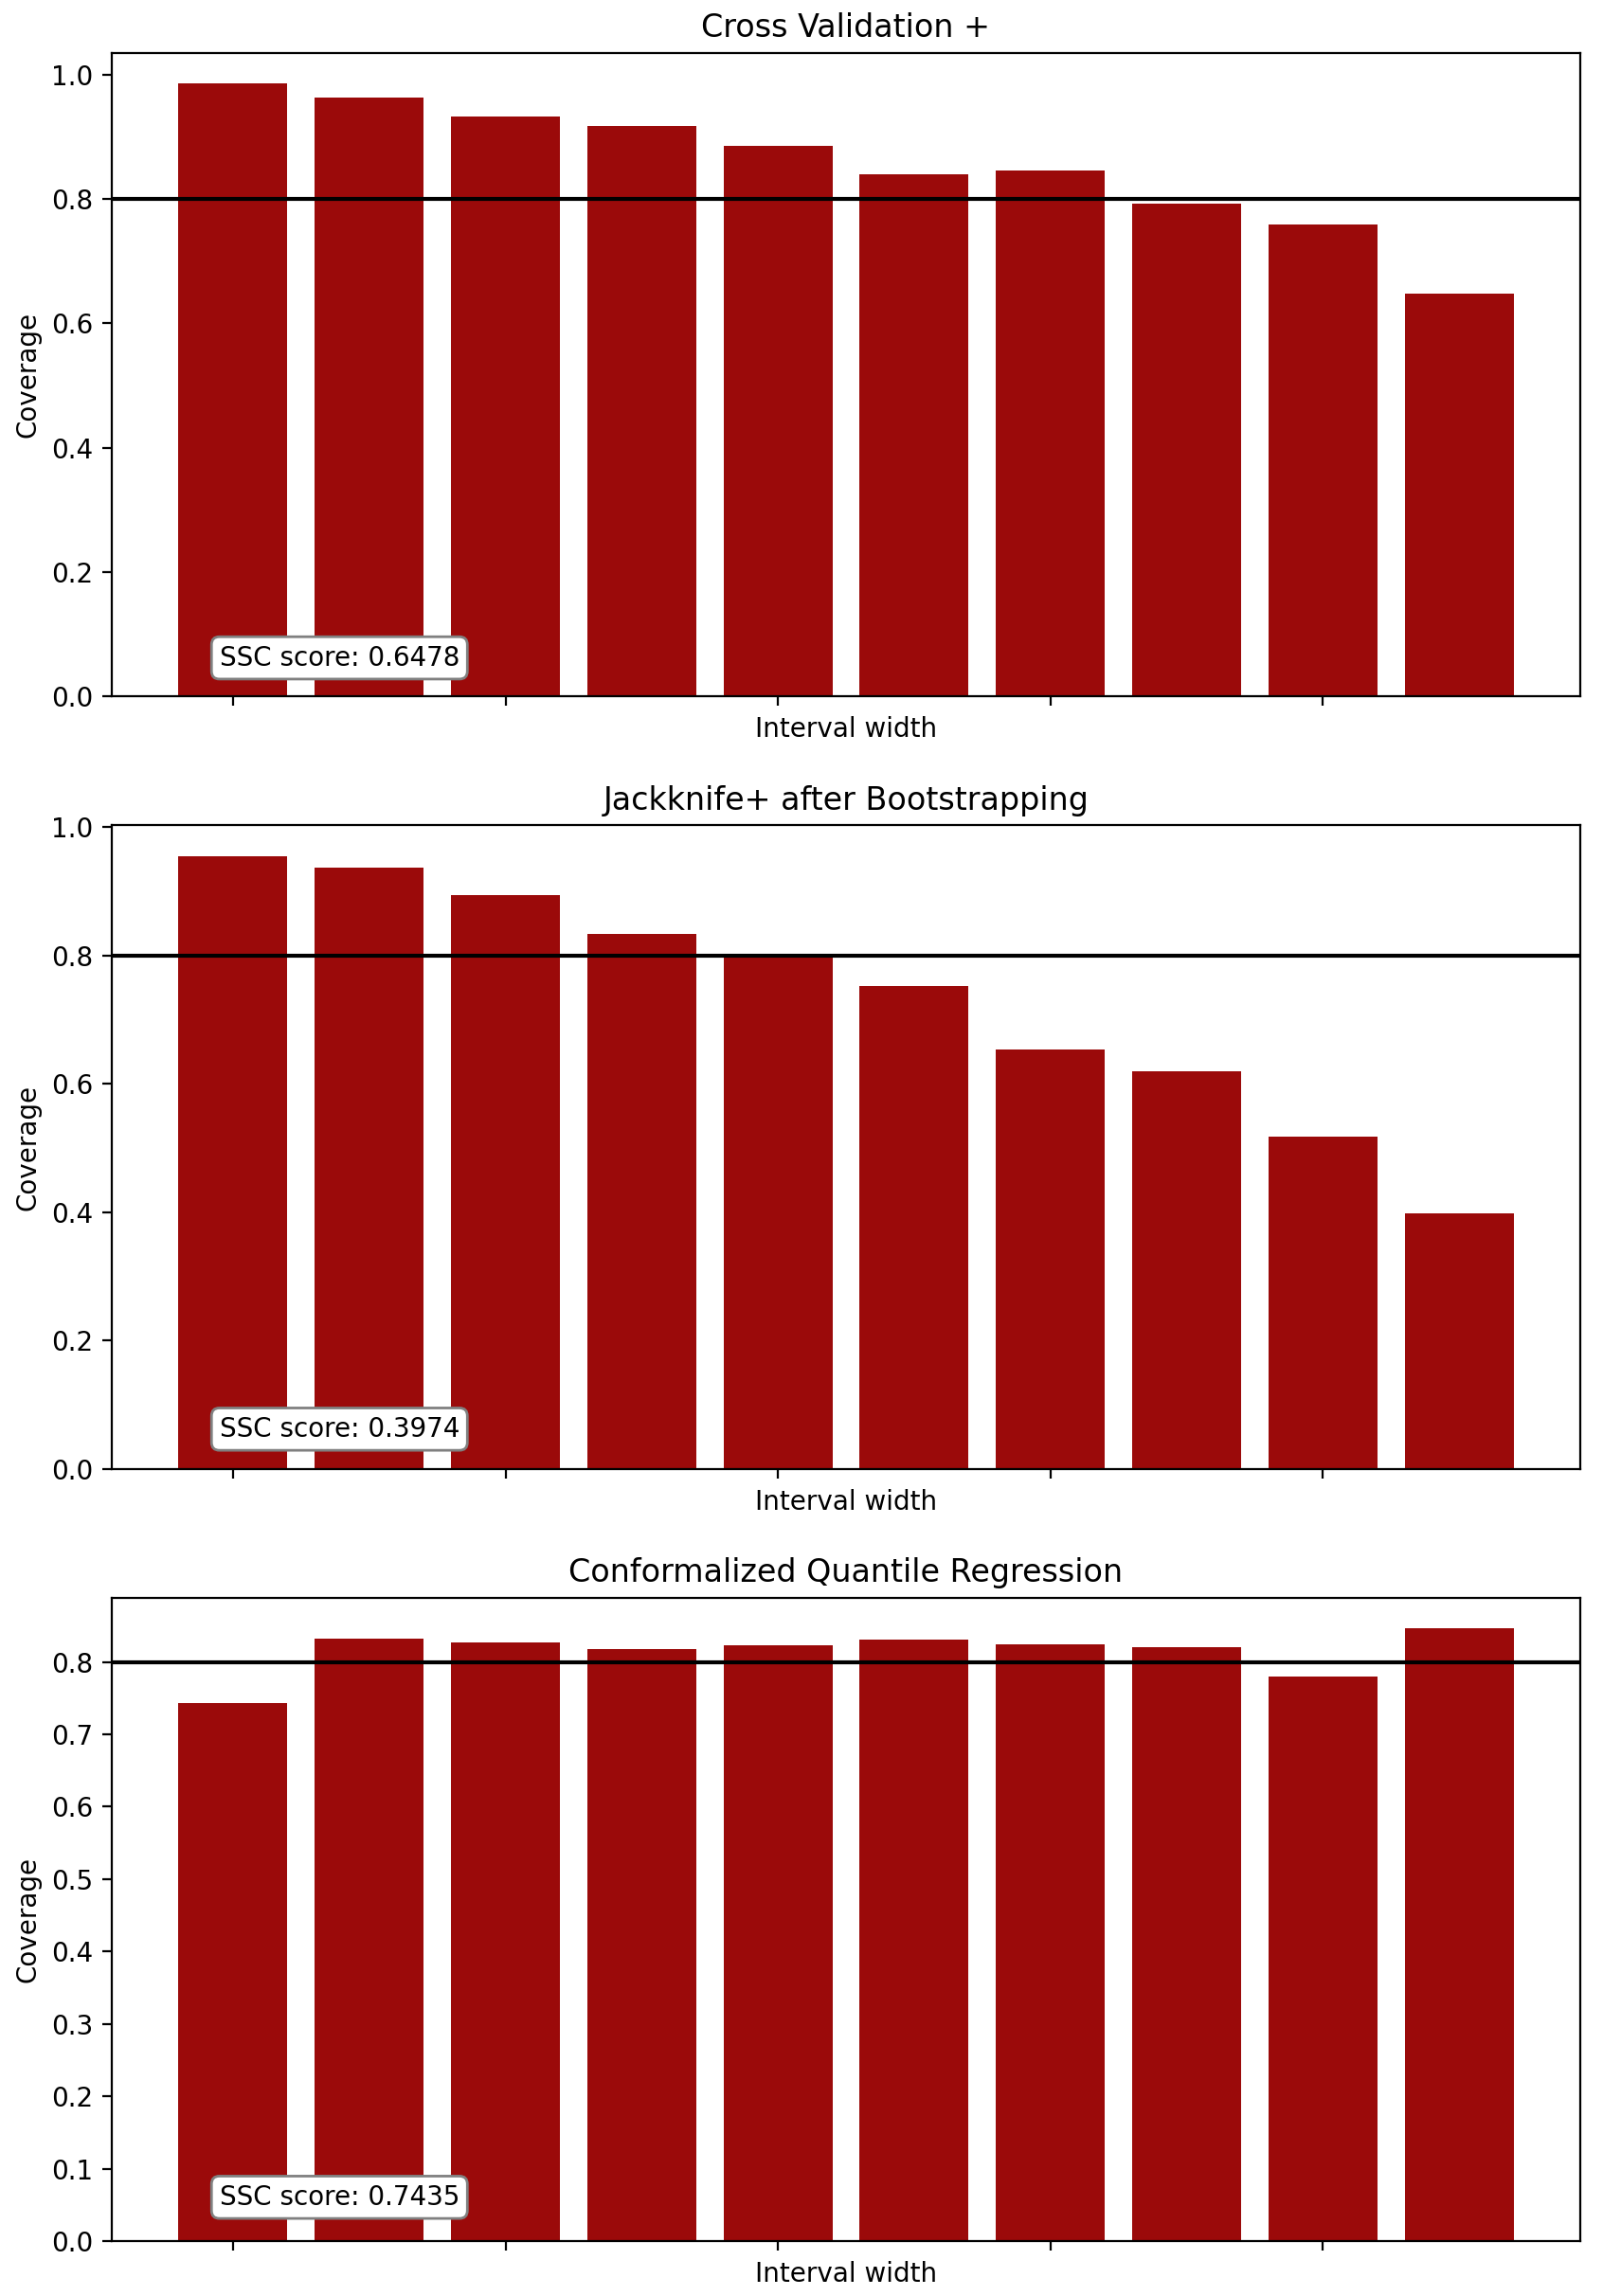
\includegraphics[width=1.15\textwidth, height=2.95\textwidth]{Figures/regression/coverage-vs-width-regression-problem.png}
        \caption{Coverage in function of intervals' width}
        \label{subfig:app-regression-coverage-width}
    \end{subfigure}
    \hfill % adds horizontal space between figures
    \begin{subfigure}[b]{0.32\textwidth} % Adjust the width to fit your needs
        \centering
        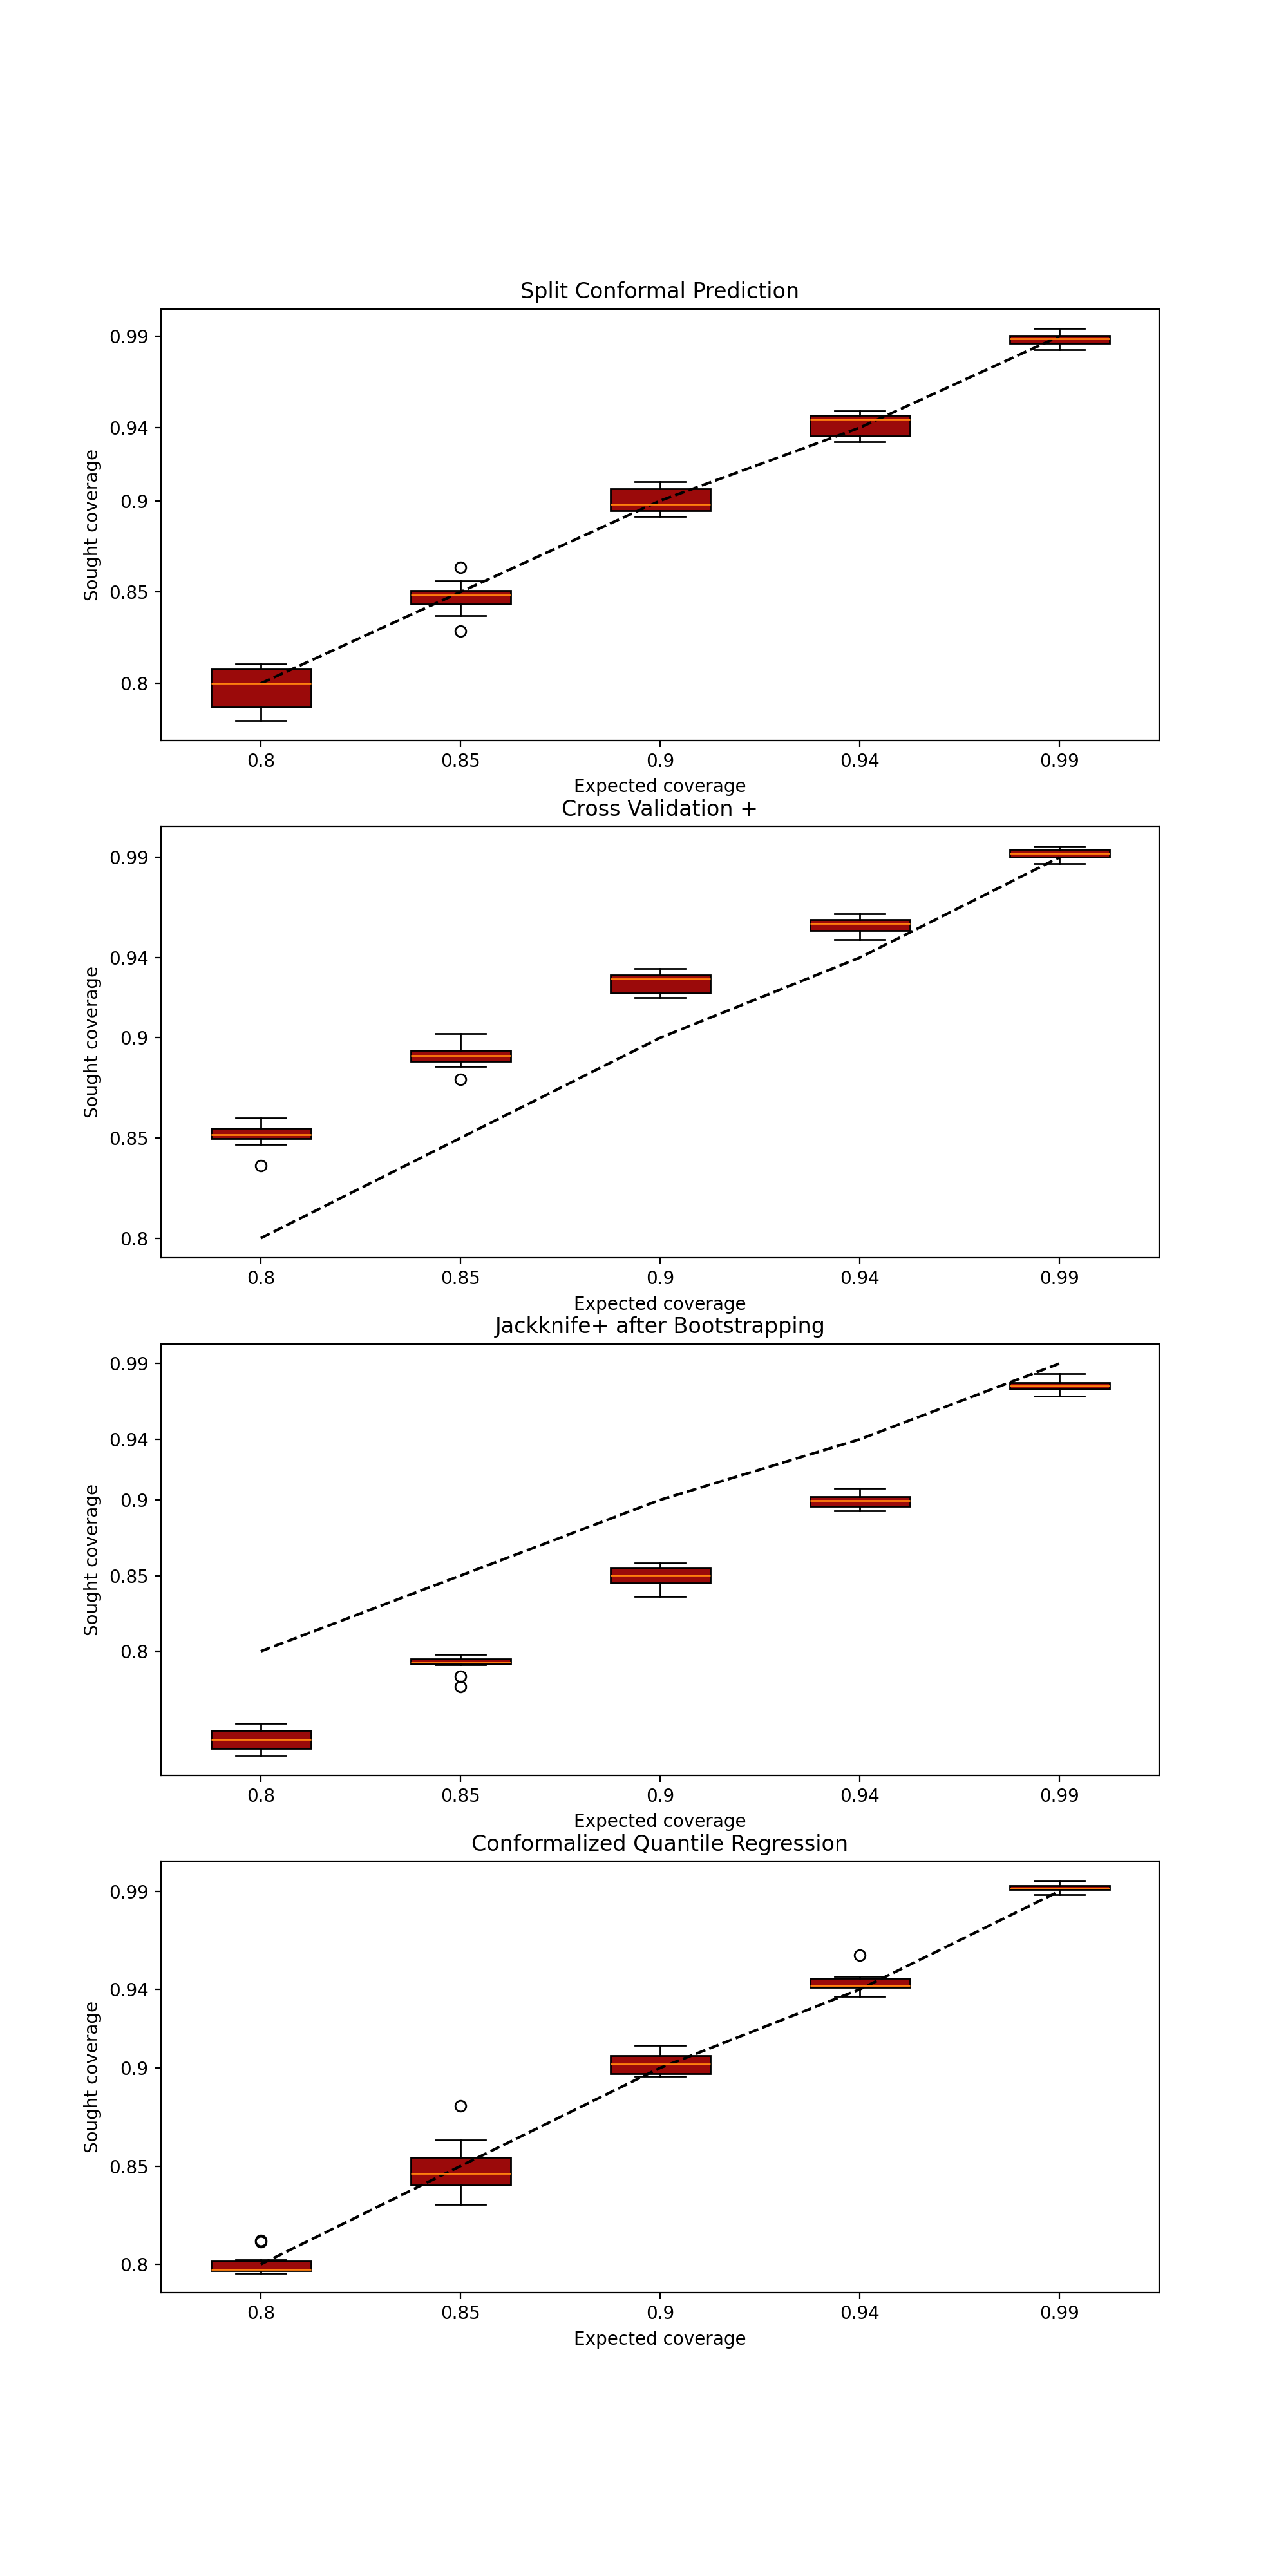
\includegraphics[width=1.15\textwidth, height=4\textwidth]{Figures/regression/coverage-vs-alpha-regression-problem.png} % Adjust the filename and path
        \caption{Coverage in function of $\a$}
        \label{subfig:app-regression-coverage-alpha}
    \end{subfigure}
    \caption{Visualizations related to width \& coverage distributions for the test data and 4 different strategies; from top to bottom: SCP, CV$+$, J$+$aB \& CQR. The first 2 plots just display the last 3 strategies, since SCP displays no adaptability at all (whereas J$+$aB slight to none adaptability).}
    \label{fig:app-regression-width-coverage}
\end{figure}

\begin{figure}[ht]
    \centering
    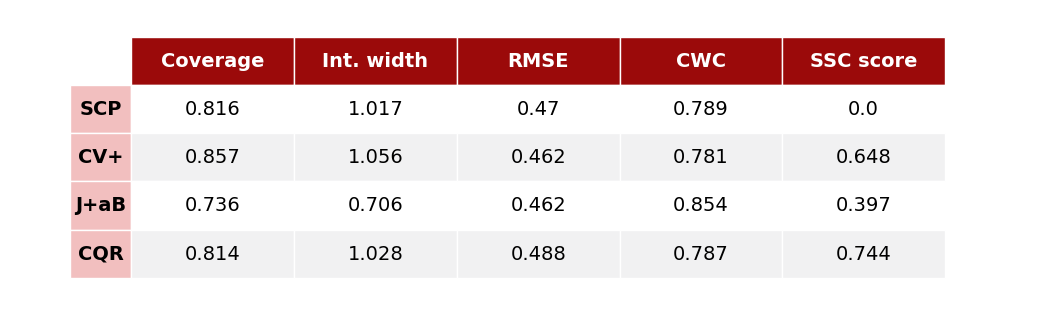
\includegraphics[width=\textwidth]{Figures/regression/metrics-table-regression-problem.png}
    \caption{Test data metrics for the 4 different strategies and 1 particular experiment (no 5-folds CV) for $\a=0.20$. From top to bottom: SCP, CV$+$, J$+$aB and CQR.}
    \label{fig:app-regression-metrics}
\end{figure}
\chapter{Time series original problem}
\label{app:timeseries-original-problem} 

Unless it is specified otherwise, the miscoverage level was set to $\a=0.2$ (\textit{i.e.} $80\%$ of expected coverage) for the visualizations.

\begin{figure}[ht]
    \centering
    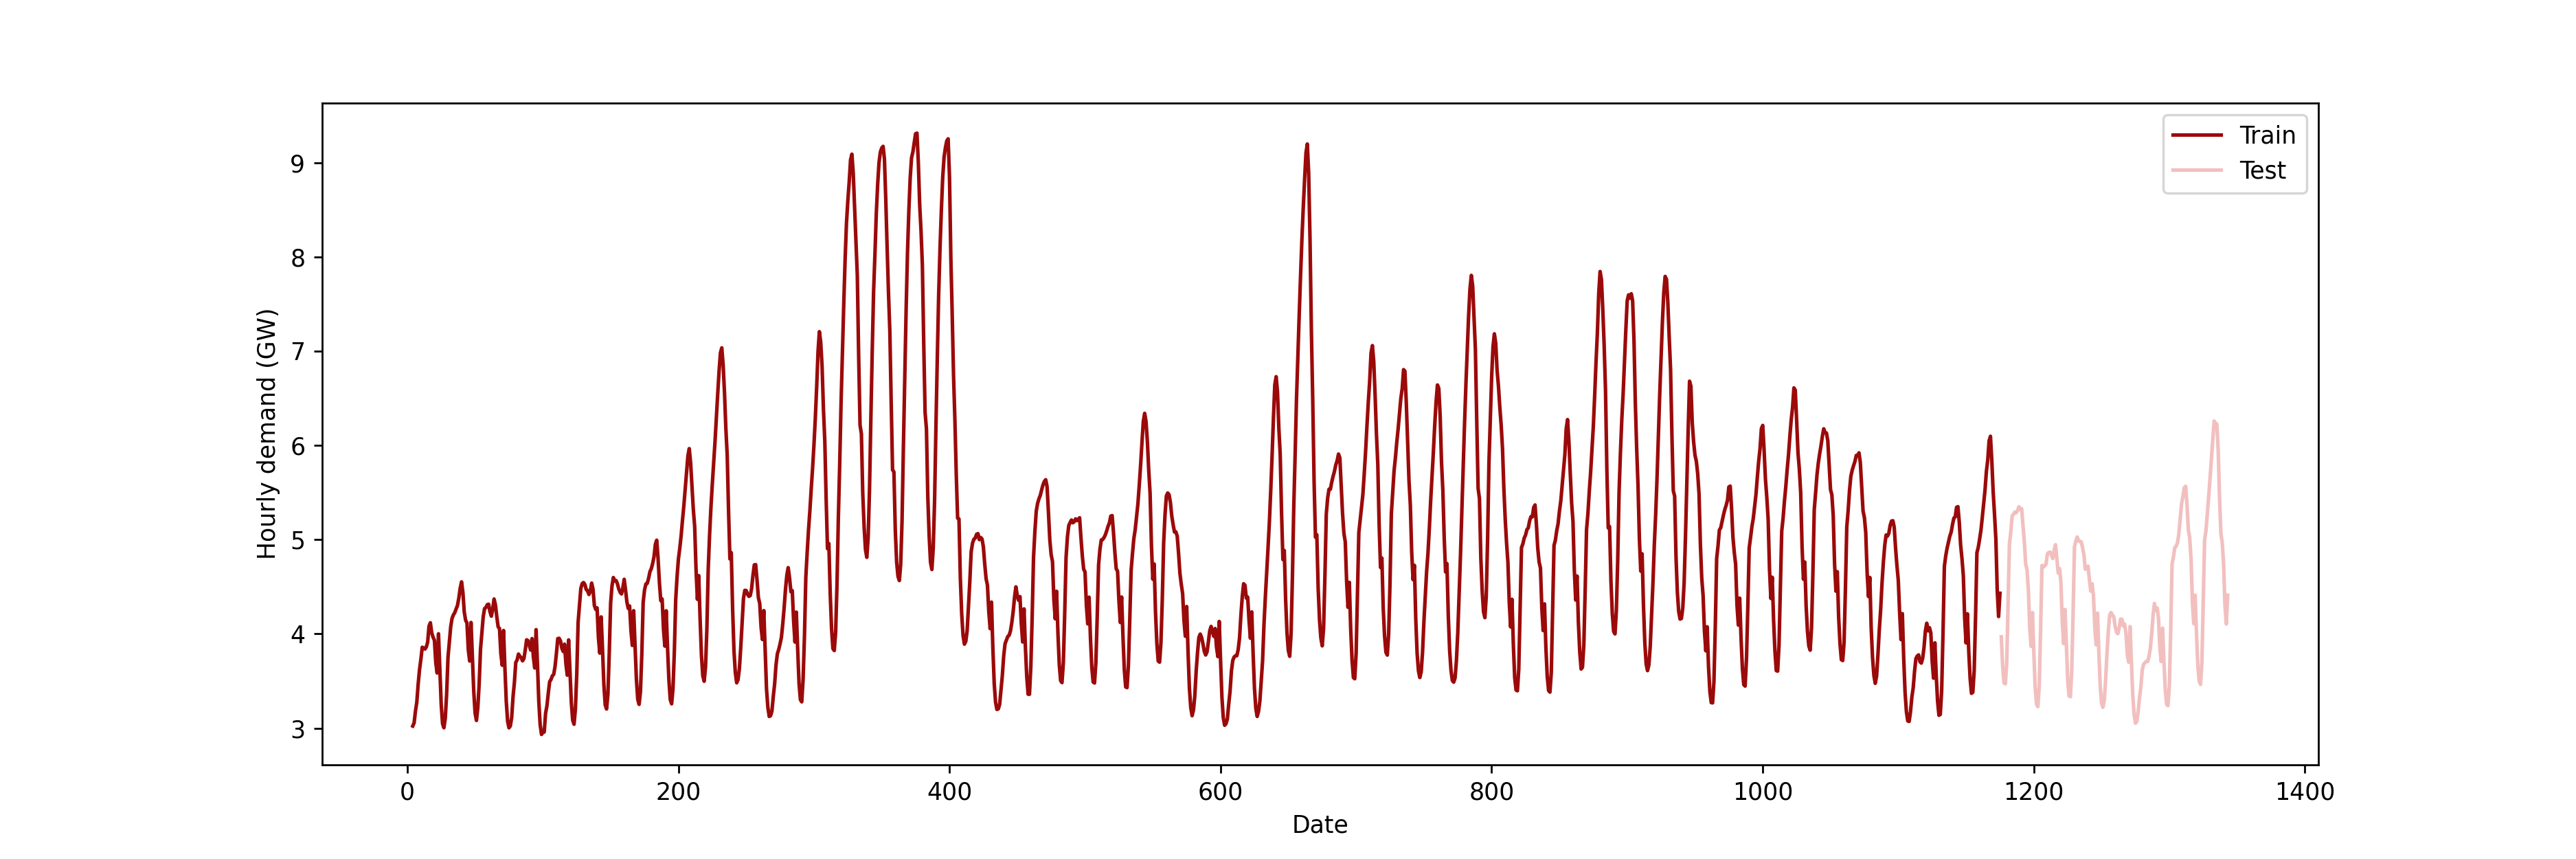
\includegraphics[width=1\textwidth]{Figures/timeseries/without-change-point/data-timeseries.png}
    \caption{Time series problem's dataset.}
    \label{fig:app-timeseries-data}
\end{figure}

\begin{figure}[ht]
    \centering
    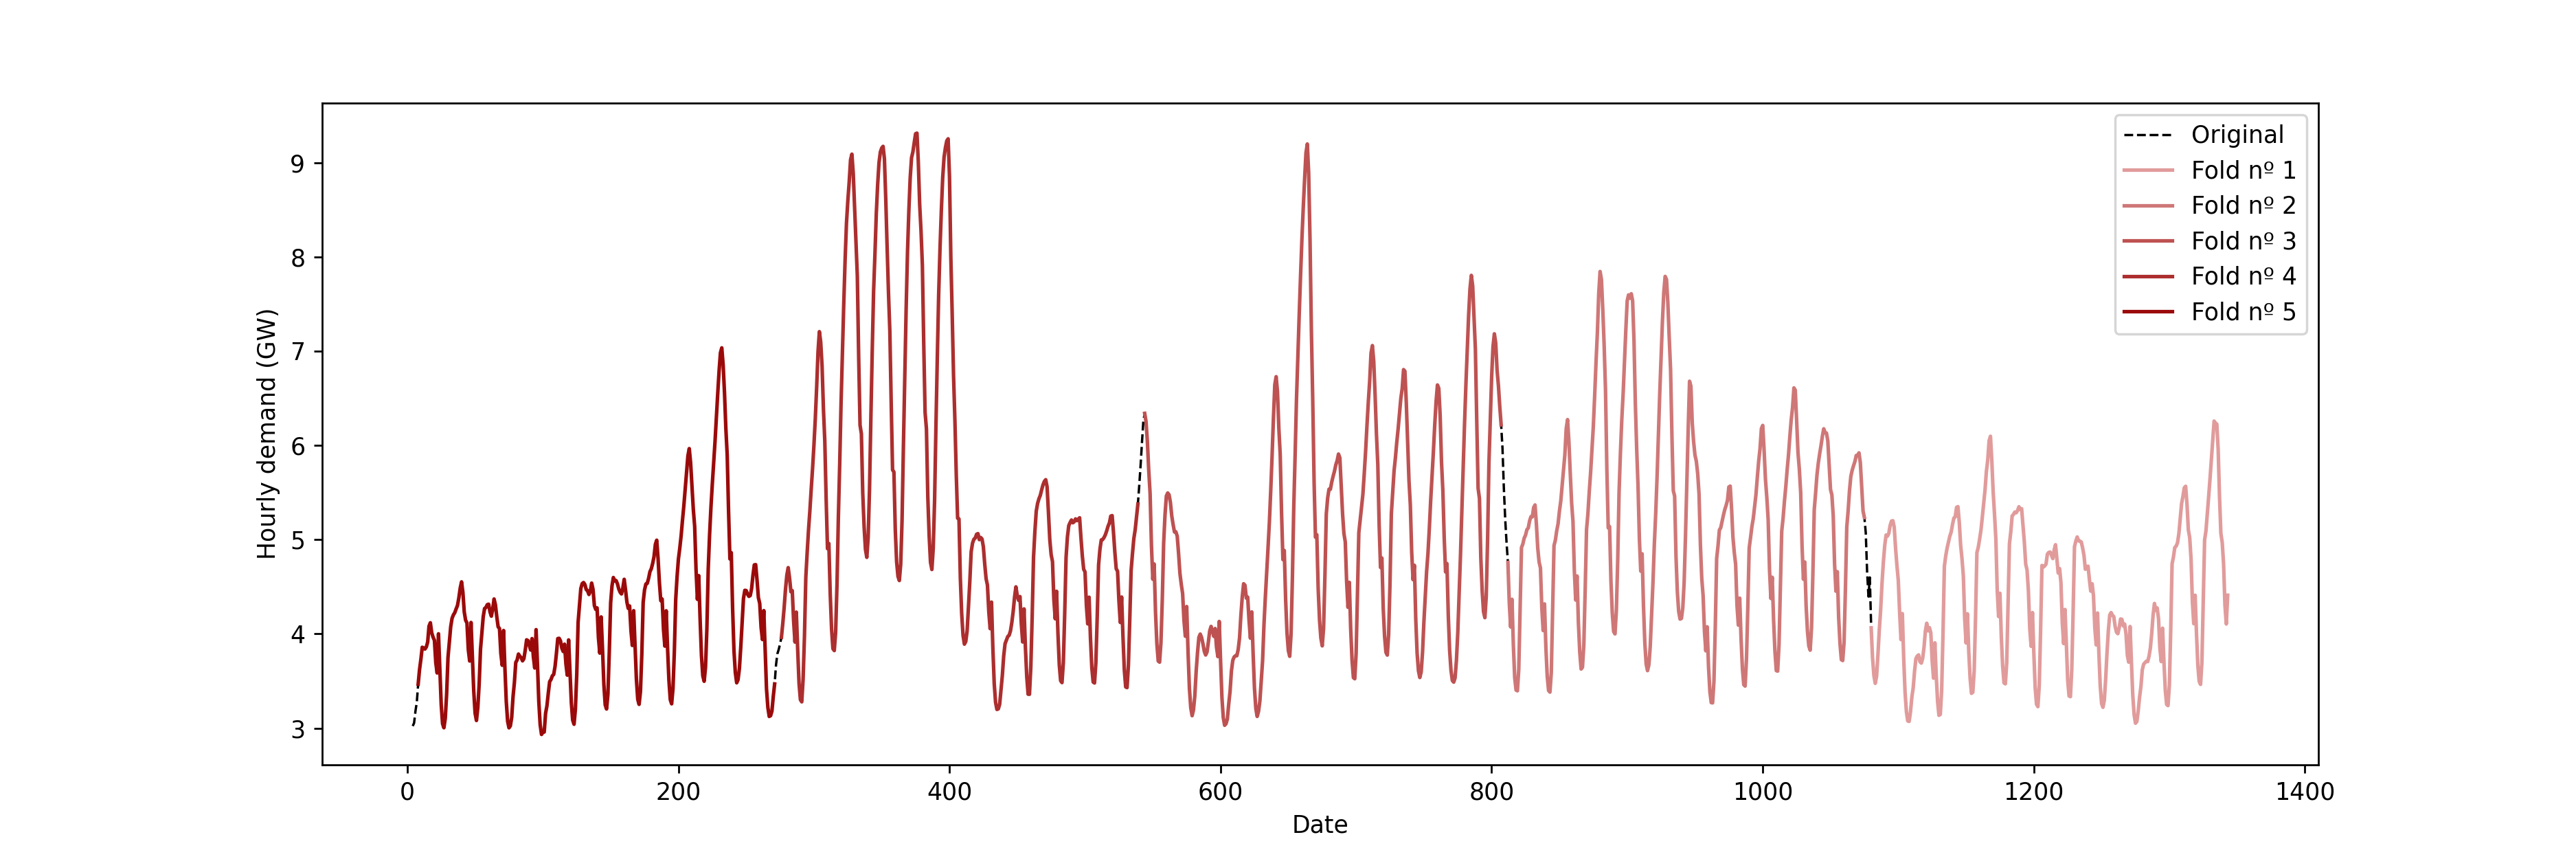
\includegraphics[width=1\textwidth]{Figures/timeseries/without-change-point/ts-5-folds.png}
    \caption{5-fold splits from the original dataset and for the assessments based on cross-validations.}
    \label{fig:app-timeseries-5-folds}
\end{figure}

\begin{figure}[ht]
    \centering
    \begin{subfigure}[b]{\textwidth}
        \centering
        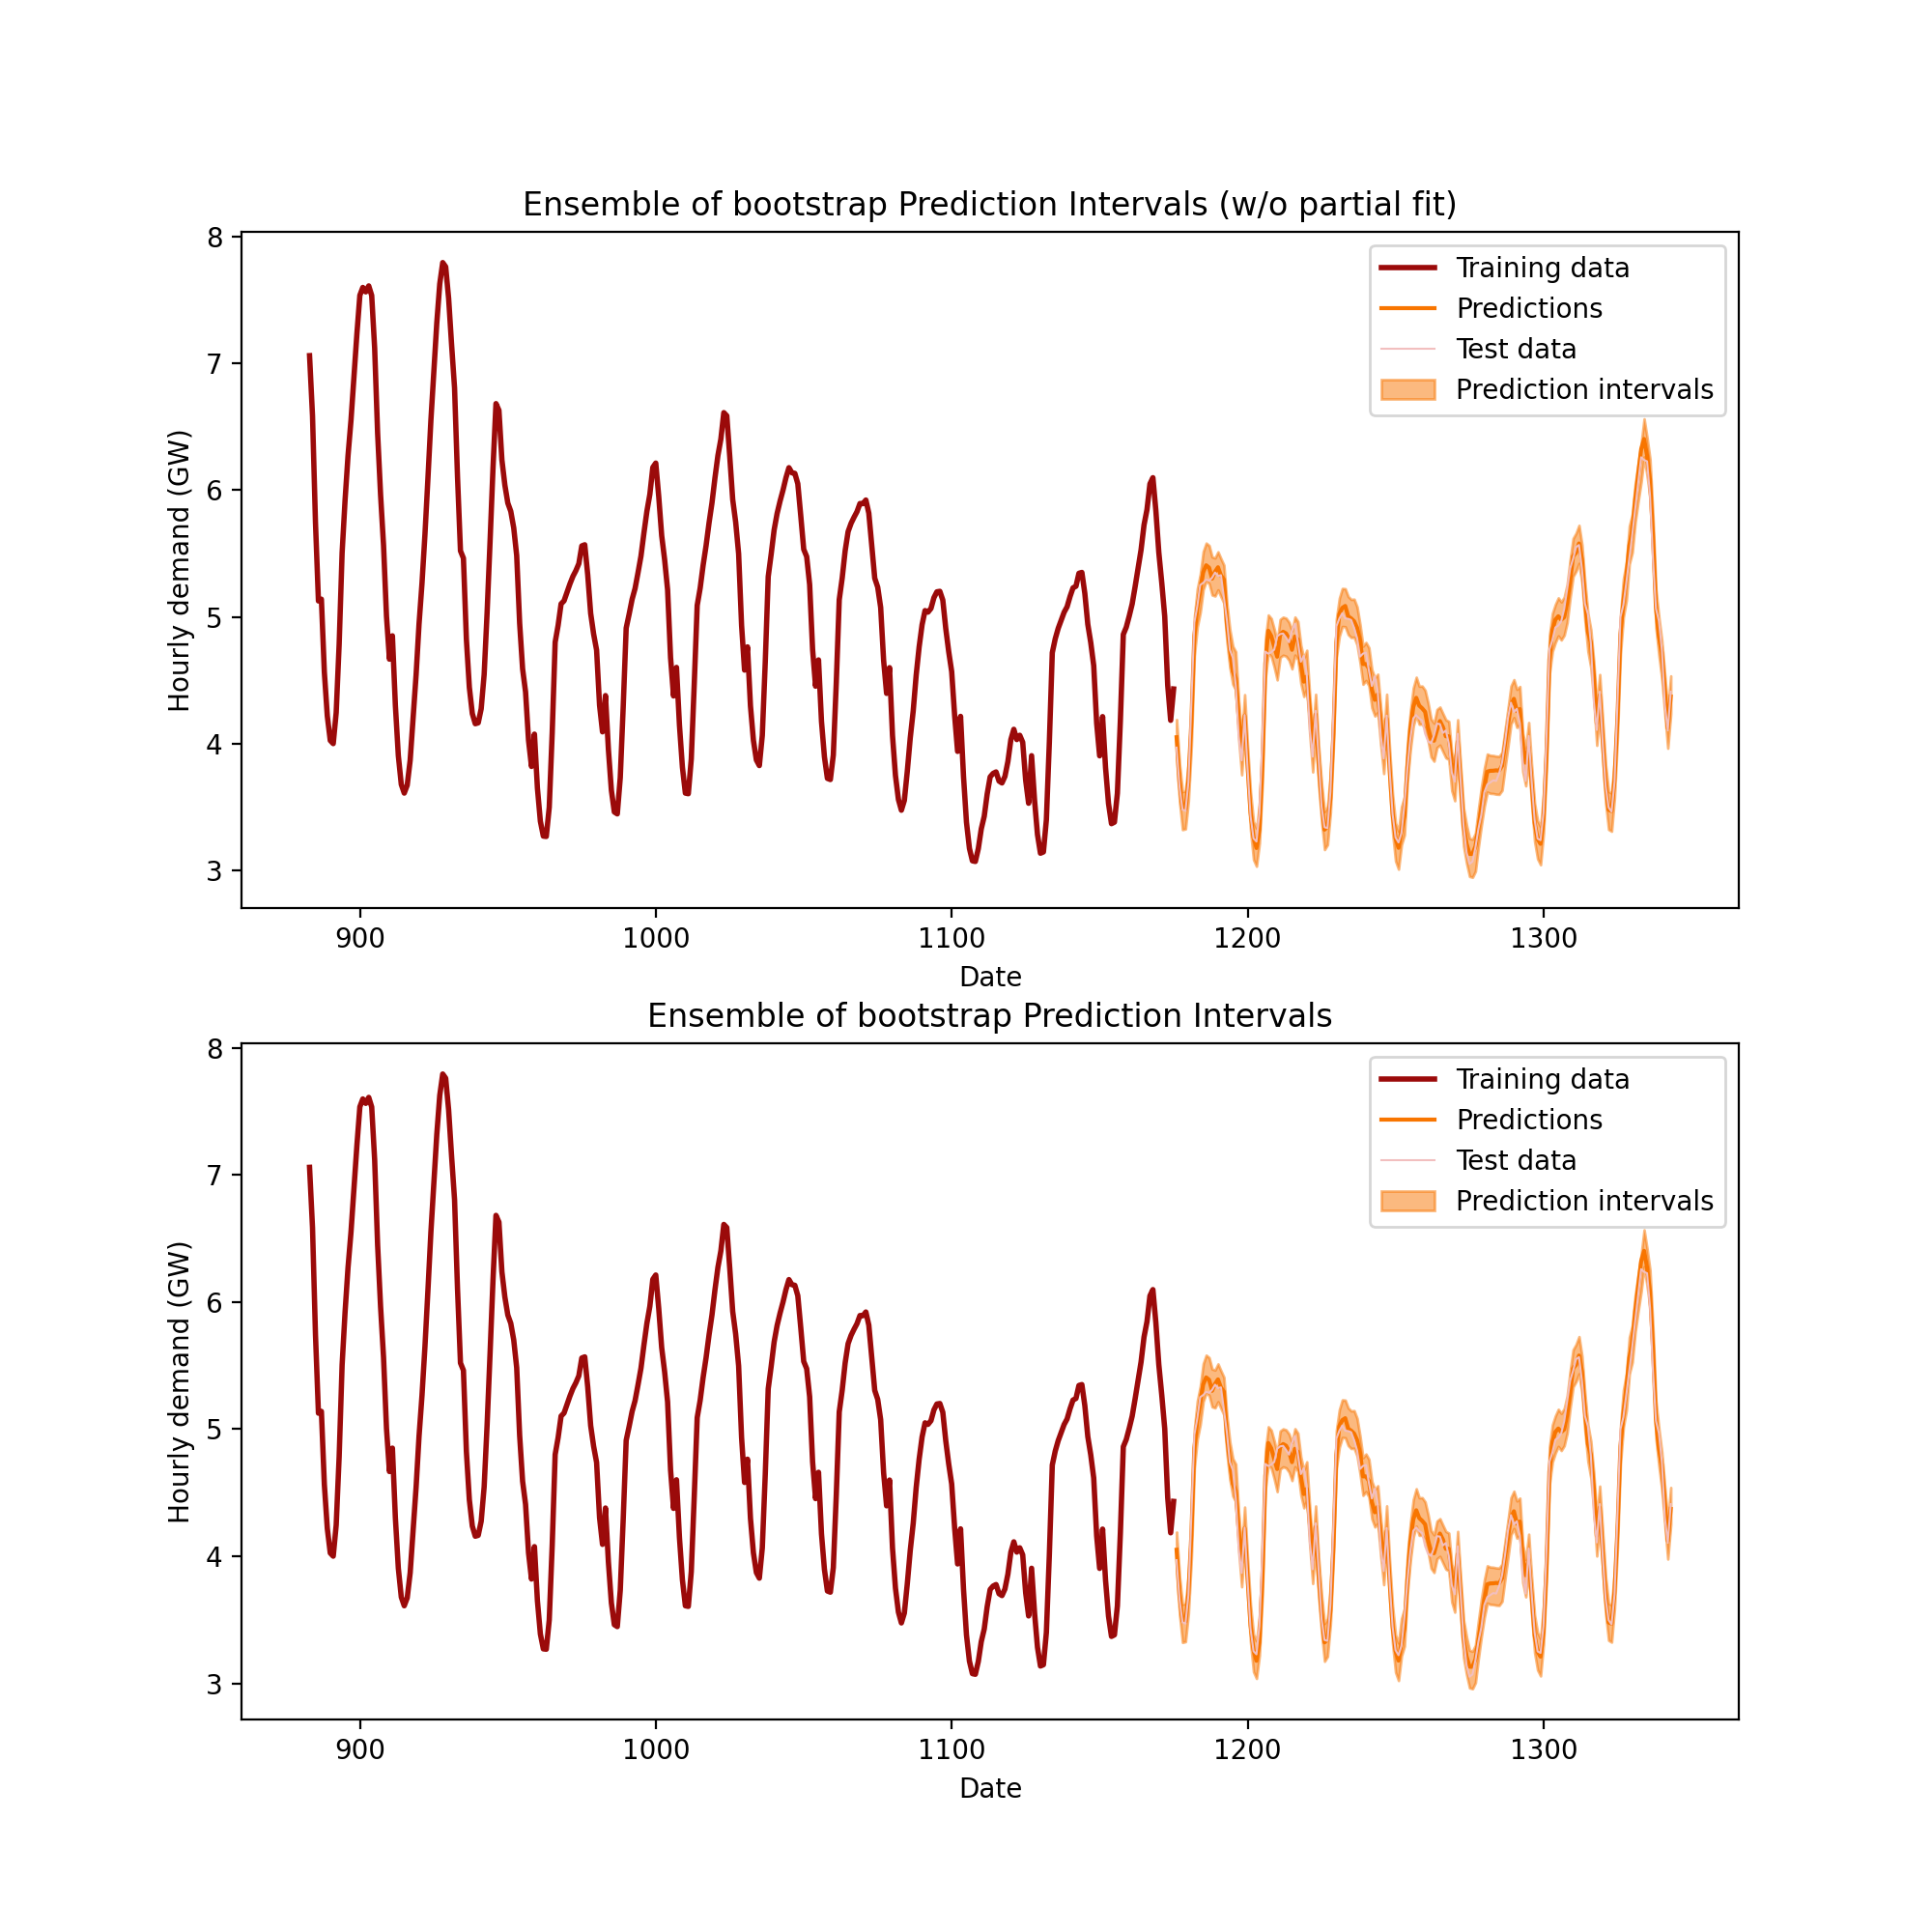
\includegraphics[width=.8\textwidth]{Figures/timeseries/without-change-point/prediction-intervals-timeseries-problem.png}
        \caption{Prediction intervals}
        \label{subfig:app-timeseries-prediction-intervals}
    \end{subfigure}
    \hfill % adds horizontal space between figures
    \begin{subfigure}[b]{\textwidth} % Adjust the width to fit your needs
        \centering
        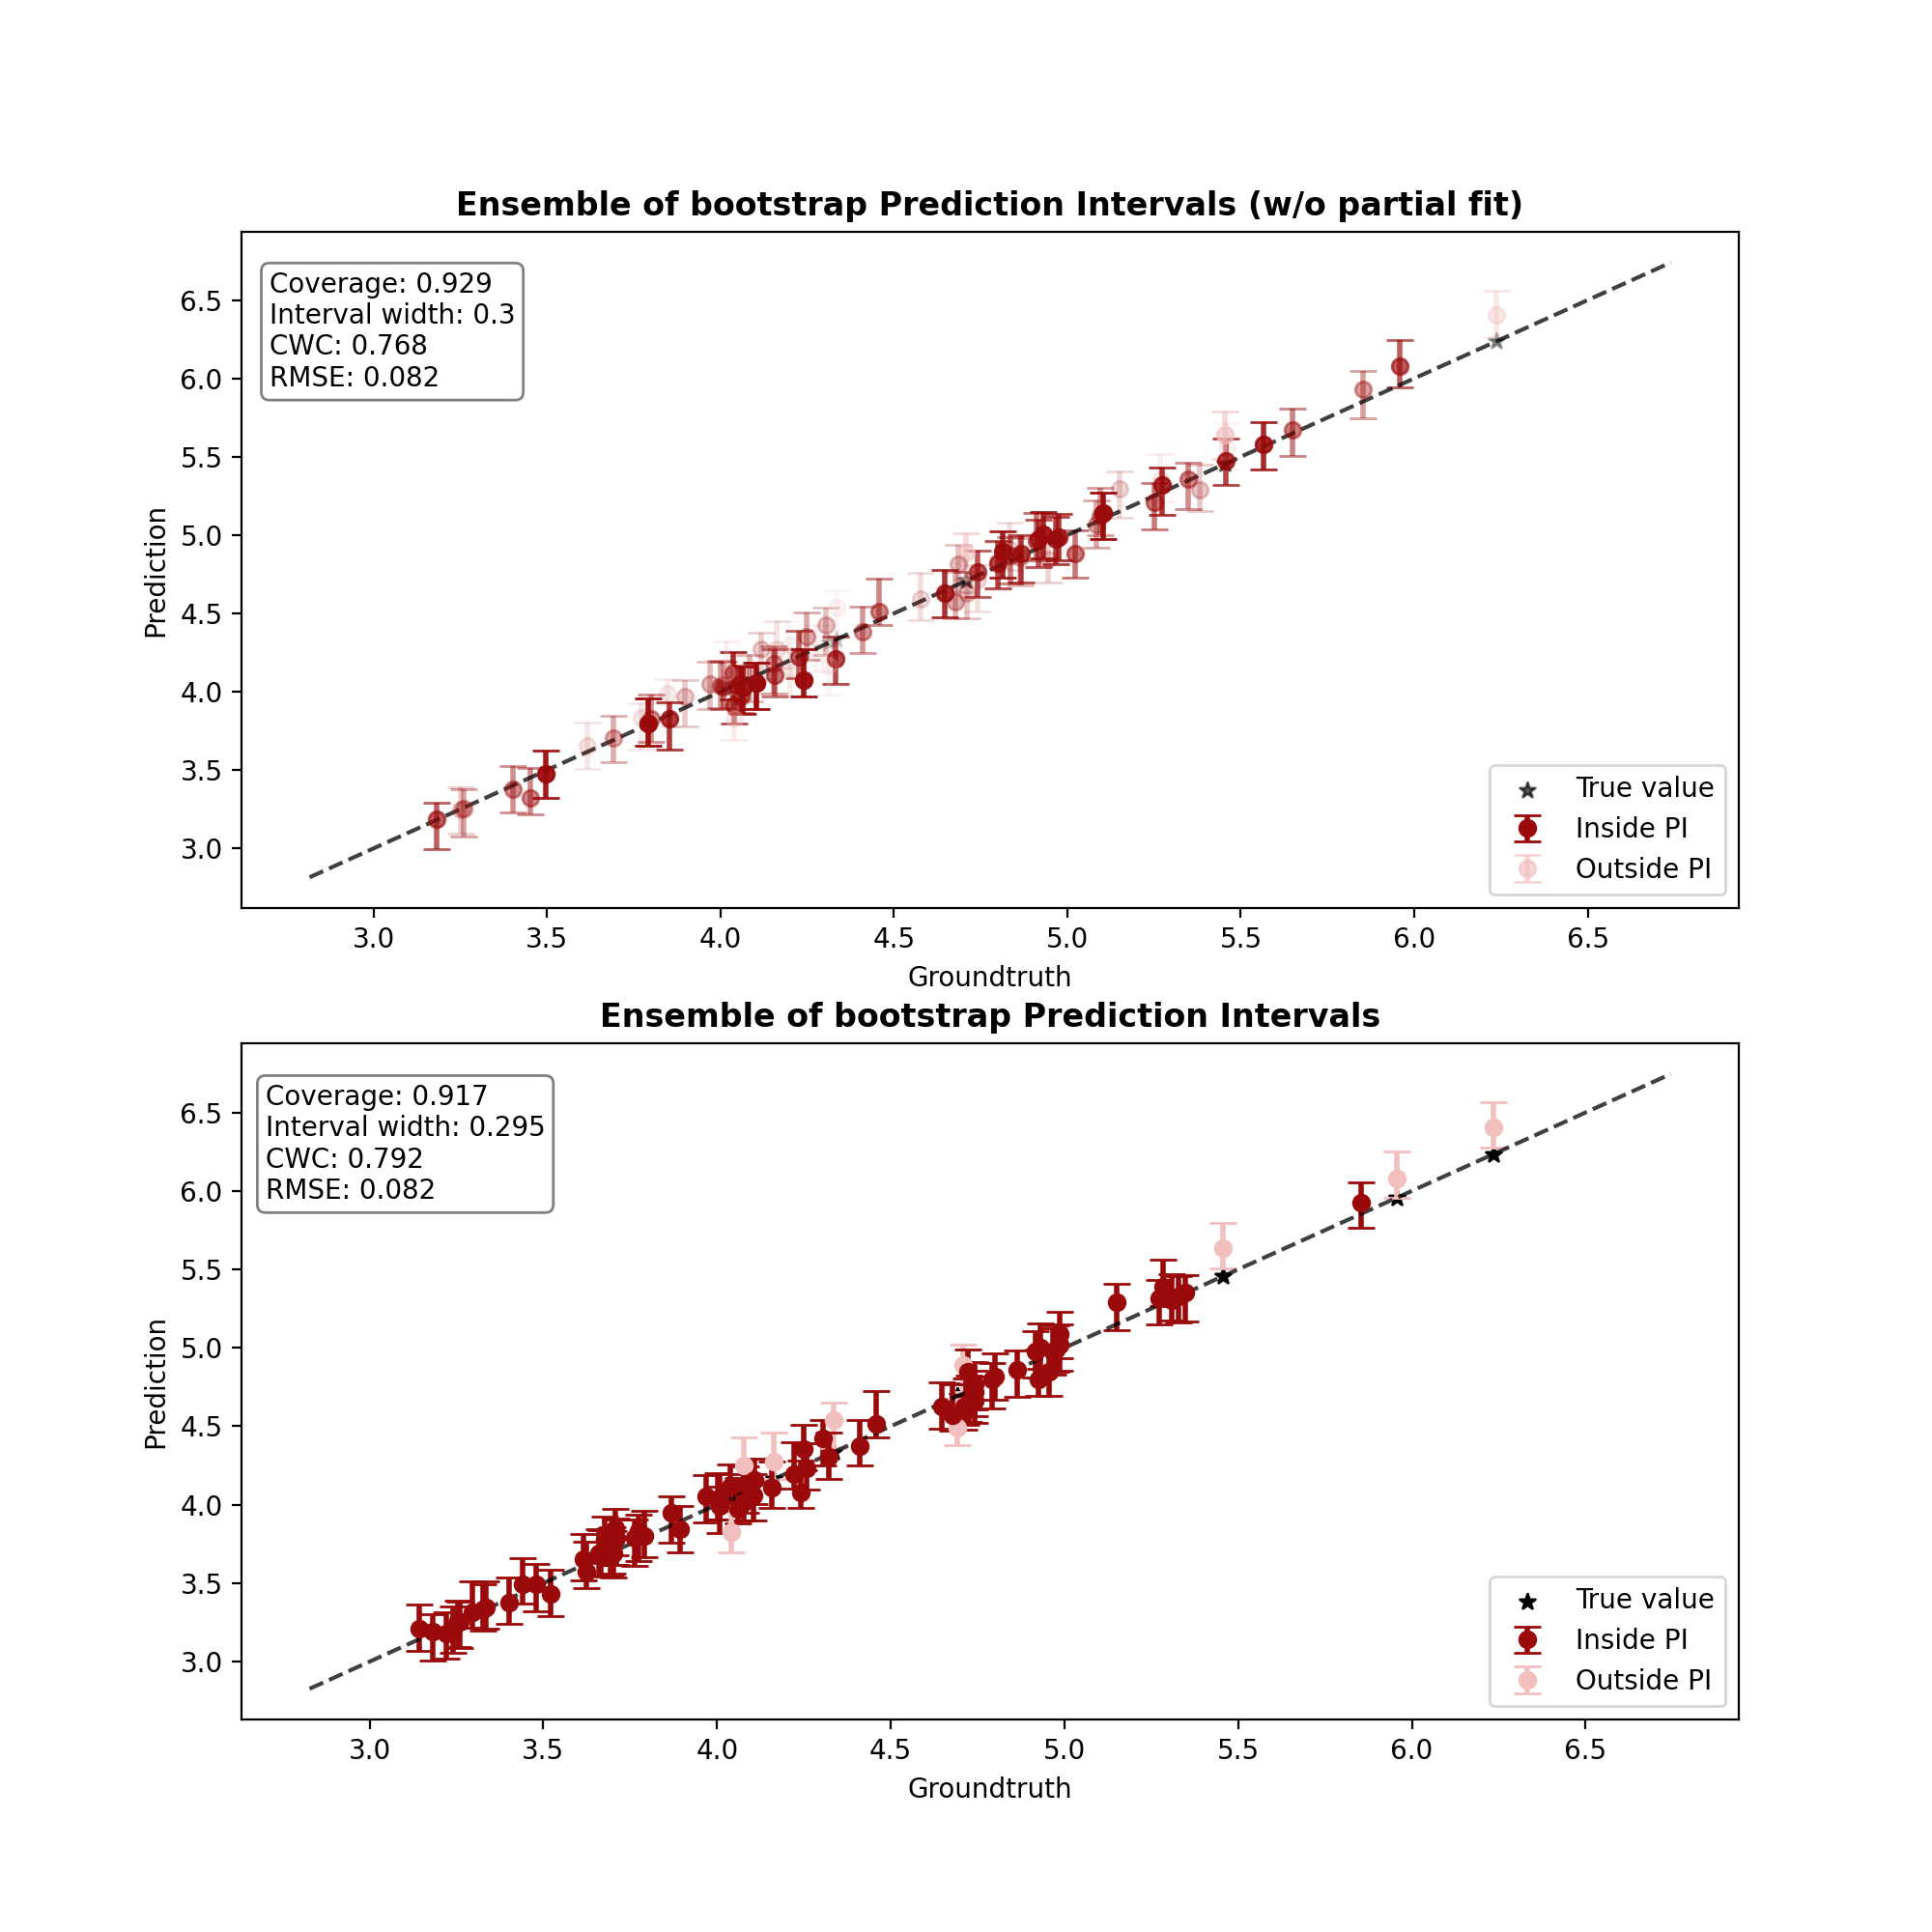
\includegraphics[width=.8\textwidth]{Figures/timeseries/without-change-point/average-goodness-timeseries-problem.png} % Adjust the filename and path
        \caption{Goodness of the prediction intervals (prediction vs. ground truth). Just a $50\%$ of the data is shown due to visualization reasons.}
        \label{subfig:app-timeseries-intervals-goodness}
    \end{subfigure}
    \caption{Visualizations related to the prediction intervals for the test data and the EnbPI strategy (without partial fit, top; and with it, bottom).}
    \label{fig:app-timeseries-intervals}
\end{figure}

\begin{figure}[ht]
    \centering
    %\hspace{-10mm}
    \begin{subfigure}[b]{0.32\textwidth}
        \centering
        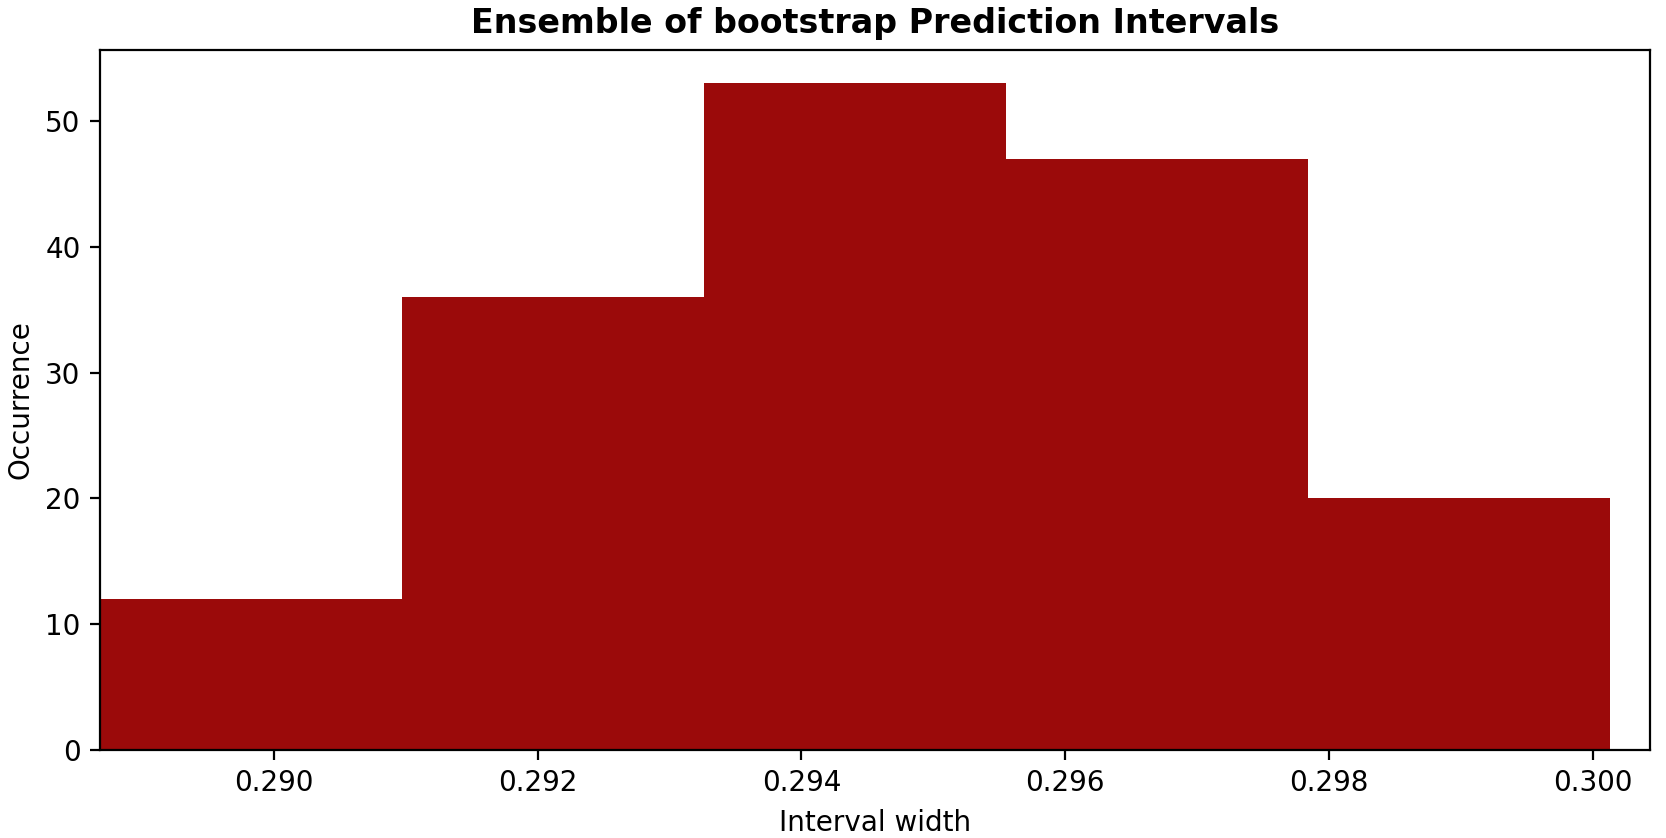
\includegraphics[width=1.15\textwidth, height=1.75\textwidth]{Figures/timeseries/without-change-point/width-occurrence-timeseries-problem.png}
        \caption{Intervals' width histograms}
        \label{subfig:app-timeseries-width-histograms}
    \end{subfigure}
    \hfill
    \begin{subfigure}[b]{0.32\textwidth}
        \centering
        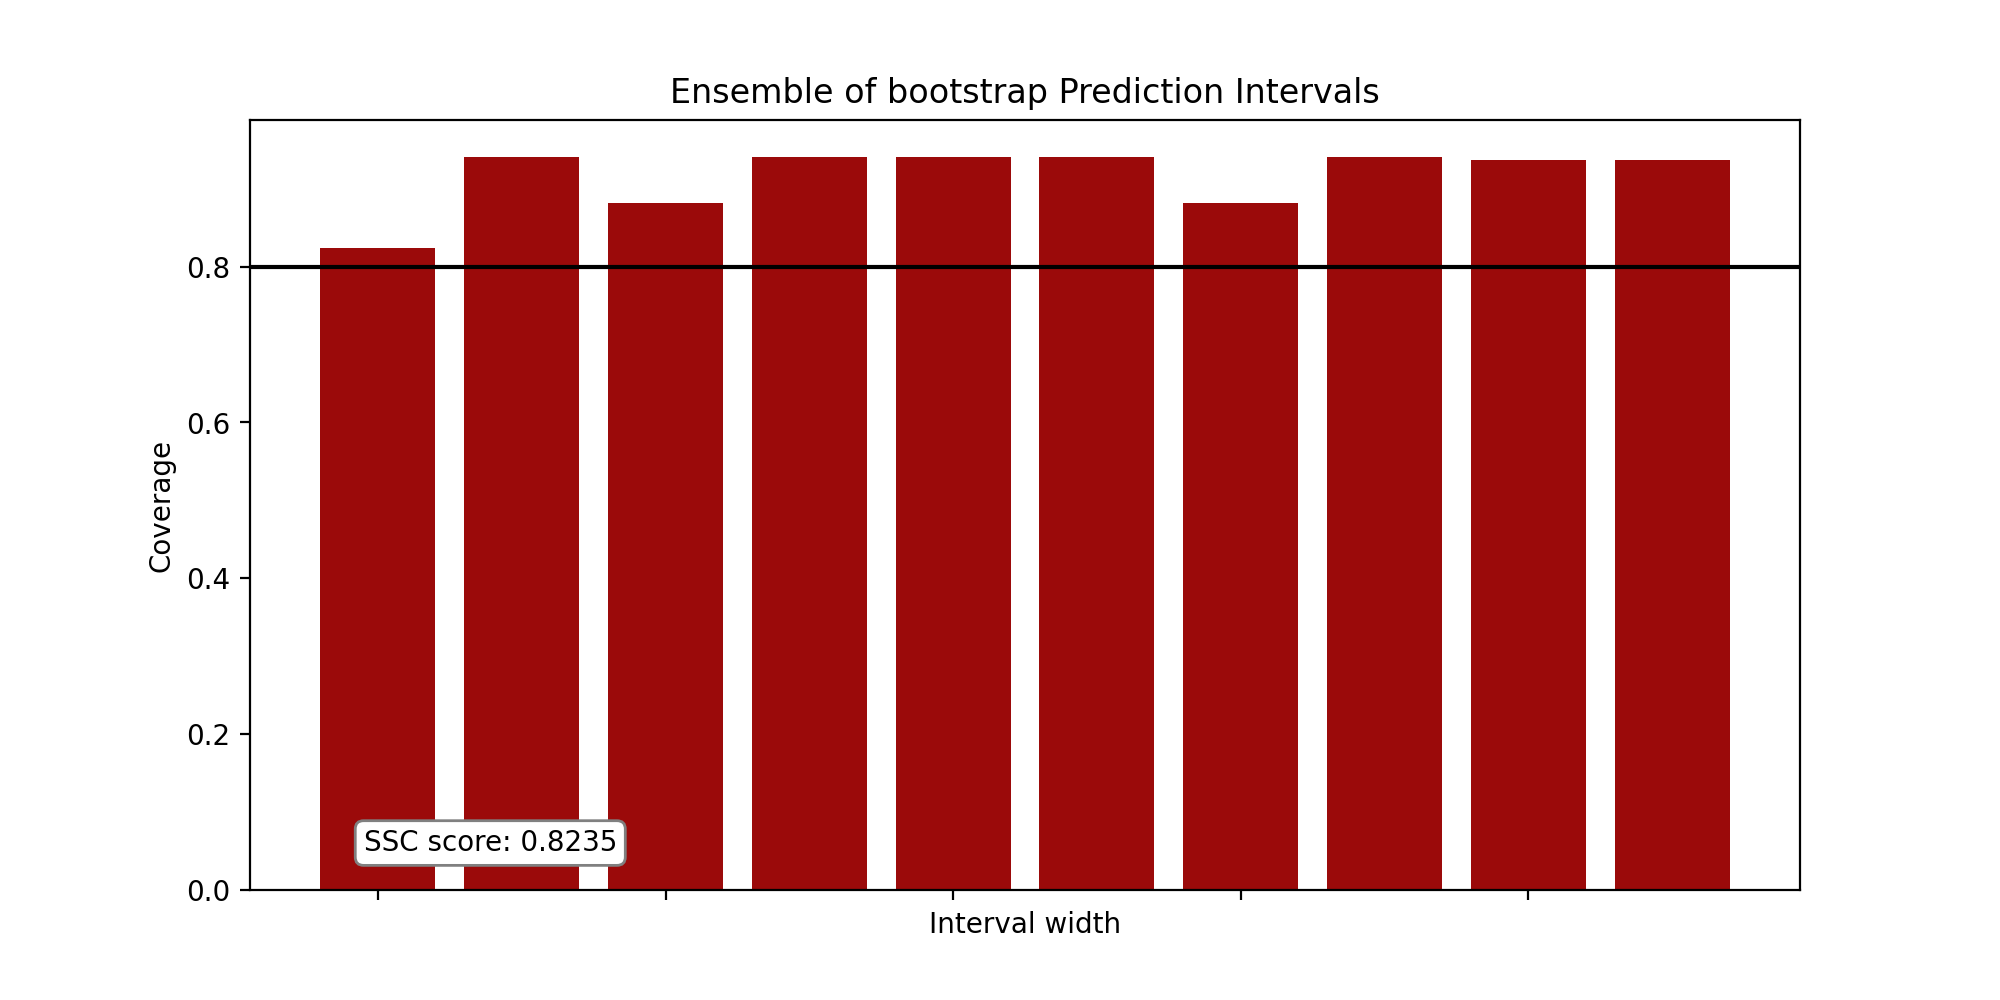
\includegraphics[width=1.15\textwidth, height=0.85\textwidth]{Figures/timeseries/without-change-point/coverage-vs-width-timeseries-problem.png}
        \caption{Coverage in function of intervals' width}
        \label{subfig:app-timeseries-coverage-width}
    \end{subfigure}
    \hfill % adds horizontal space between figures
    \begin{subfigure}[b]{0.32\textwidth} % Adjust the width to fit your needs
        \centering
        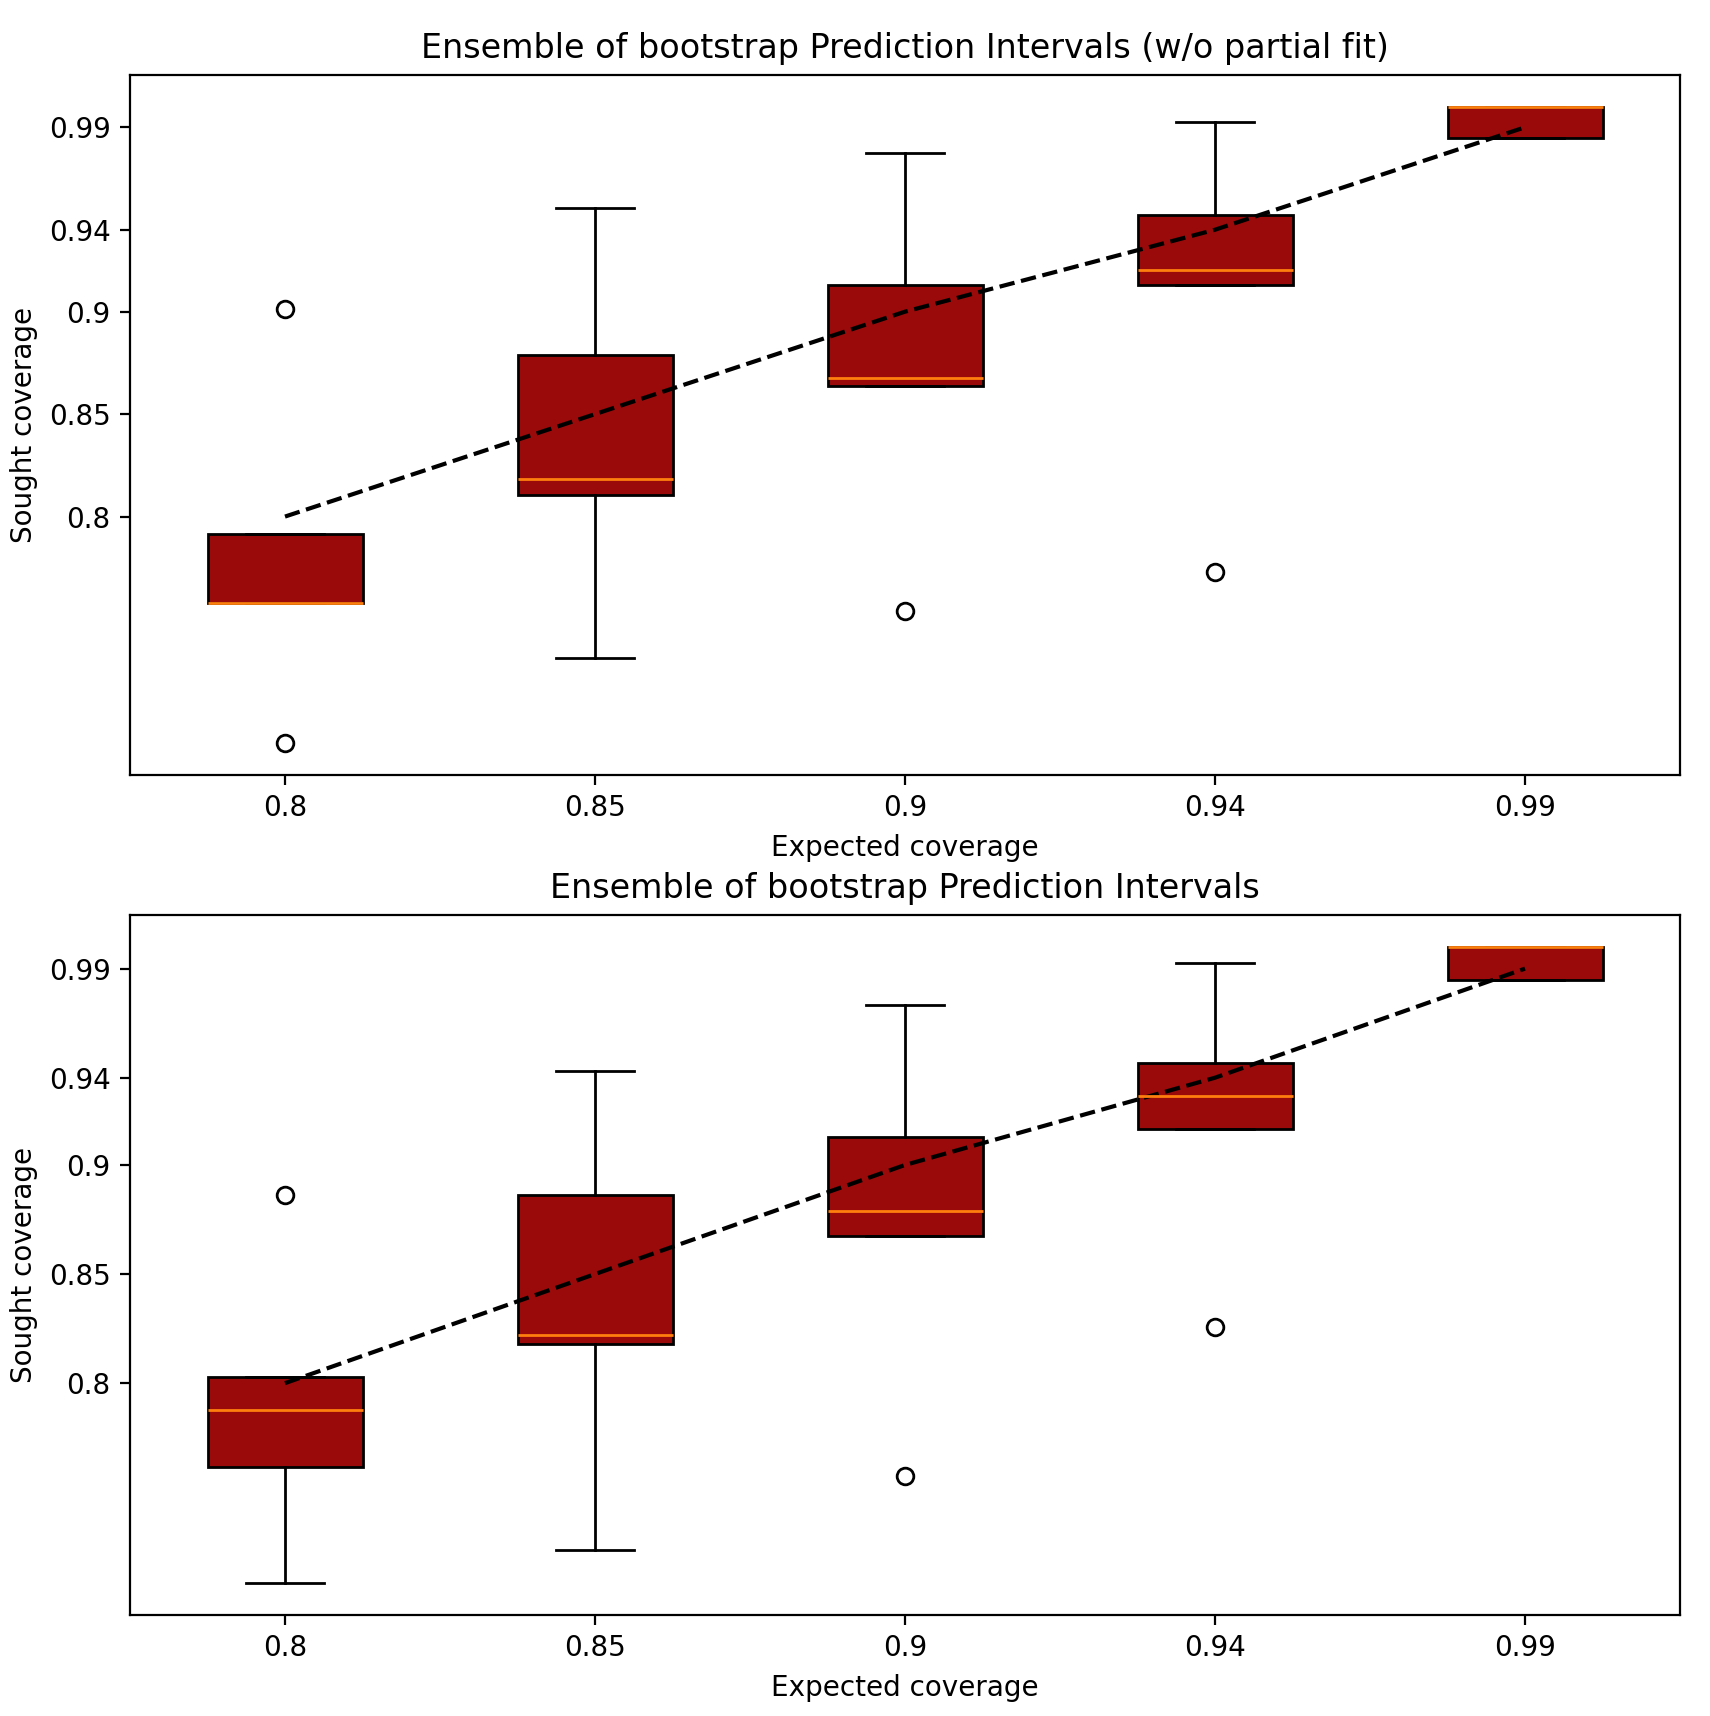
\includegraphics[width=1.15\textwidth, height=1.75\textwidth]{Figures/timeseries/without-change-point/coverage-vs-alpha-timeseries-problem.png} % Adjust the filename and path
        \caption{Coverage in function of $\a$}
        \label{subfig:app-timeseries-coverage-alpha}
    \end{subfigure}
    \caption{Visualizations related to width \& coverage distributions for the test data and the EnbPI strategy (without partial fit, top; and with it, bottom).}
    \label{fig:app-timeseries-width-coverage}
\end{figure}

\begin{figure}[ht]
    \centering
    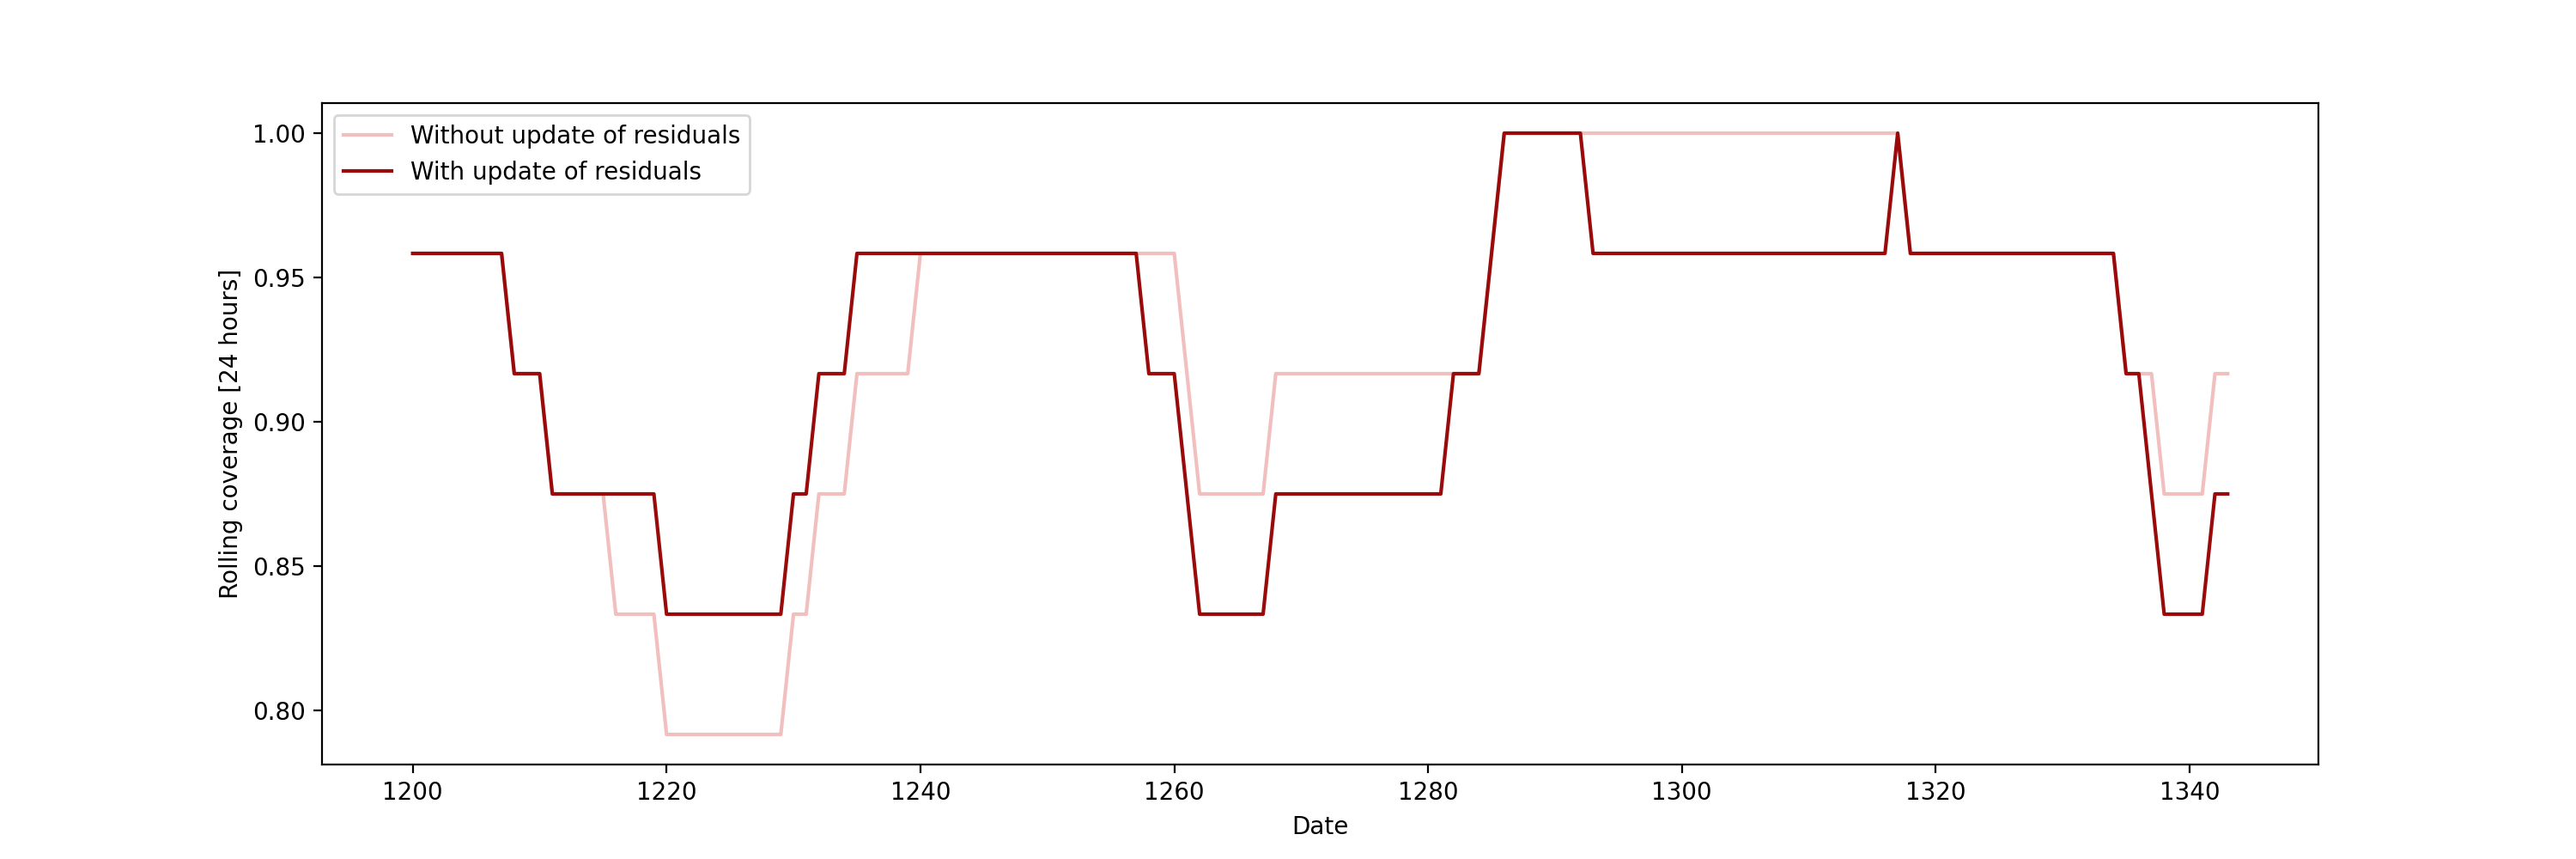
\includegraphics[width=\textwidth]{Figures/timeseries/without-change-point/rolling-coverage.png}
    \caption{Test data coverage, for the EnbPI strategies, in function of time (grouped within 24h rolling windows).}
    \label{fig:app-timeseries-rolling-coverage}
\end{figure}

\begin{figure}[ht]
    \centering
    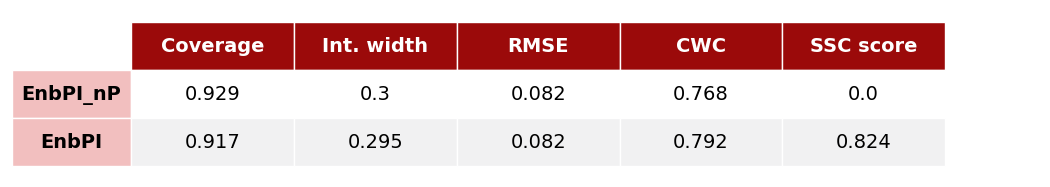
\includegraphics[width=\textwidth]{Figures/timeseries/without-change-point/metrics-table-timeseries-problem.png}
    \caption{Test data metrics for the EnbPI strategy and 1 particular experiment (no 5-folds CV) for $\a=0.20$. From top to bottom: EnbPI without partial fit (EnbPI\_{}nP), EnbPI with it (EnbPI).}
    \label{fig:app-timeseries-metrics}
\end{figure}
\chapter{Time series problem with change point in test}
\label{app:timeseries-cpoint-problem} 

Unless it is specified otherwise, the miscoverage level was set to $\a=0.05$ (\textit{i.e.} $95\%$ of expected coverage) for the visualizations.

\begin{figure}[ht]
    \centering
    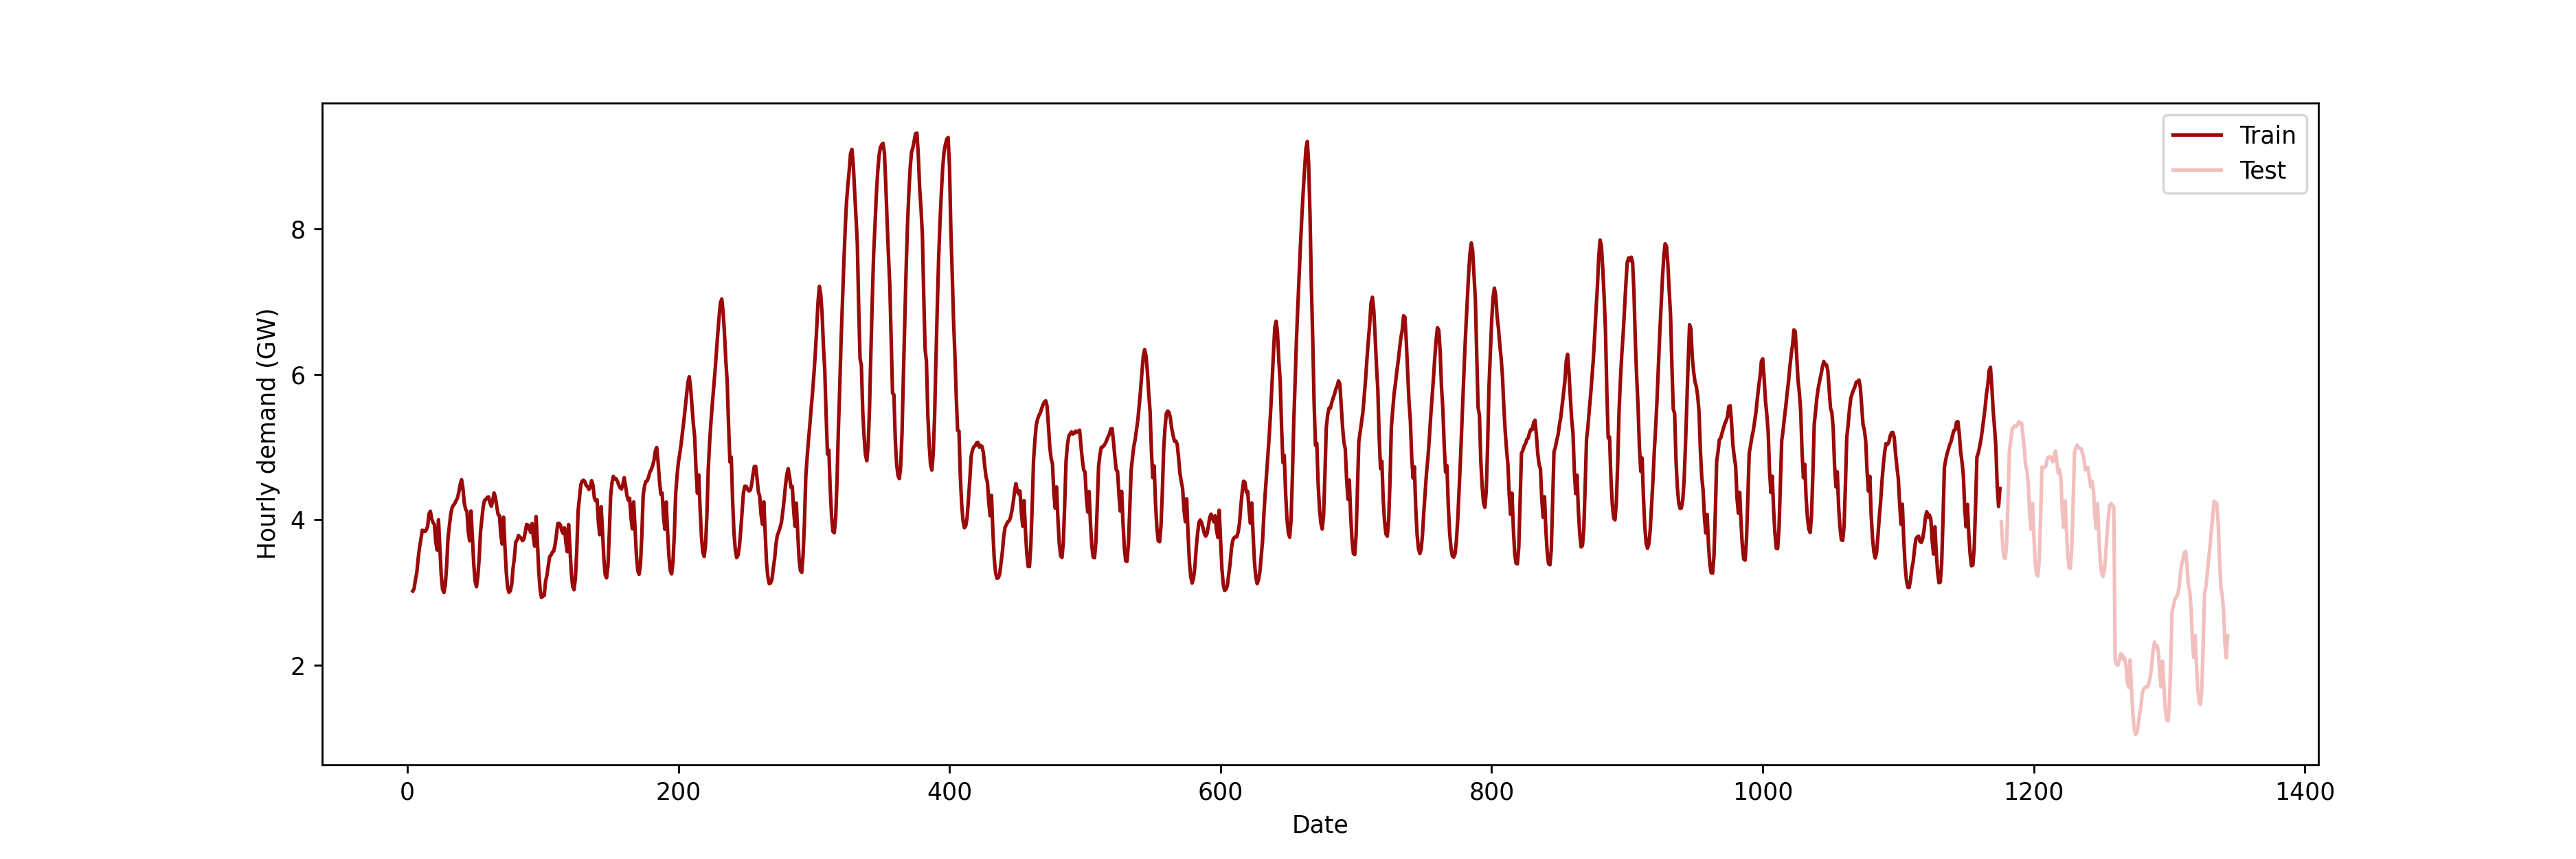
\includegraphics[width=1\textwidth]{Figures/timeseries/with-change-point/data-with-change-point-timeseries.png}
    \caption{Time series problem's dataset when a change point is added to the test split.}
    \label{fig:app-timeseries-data-cpoint}
\end{figure}

\begin{figure}[ht]
    \centering
    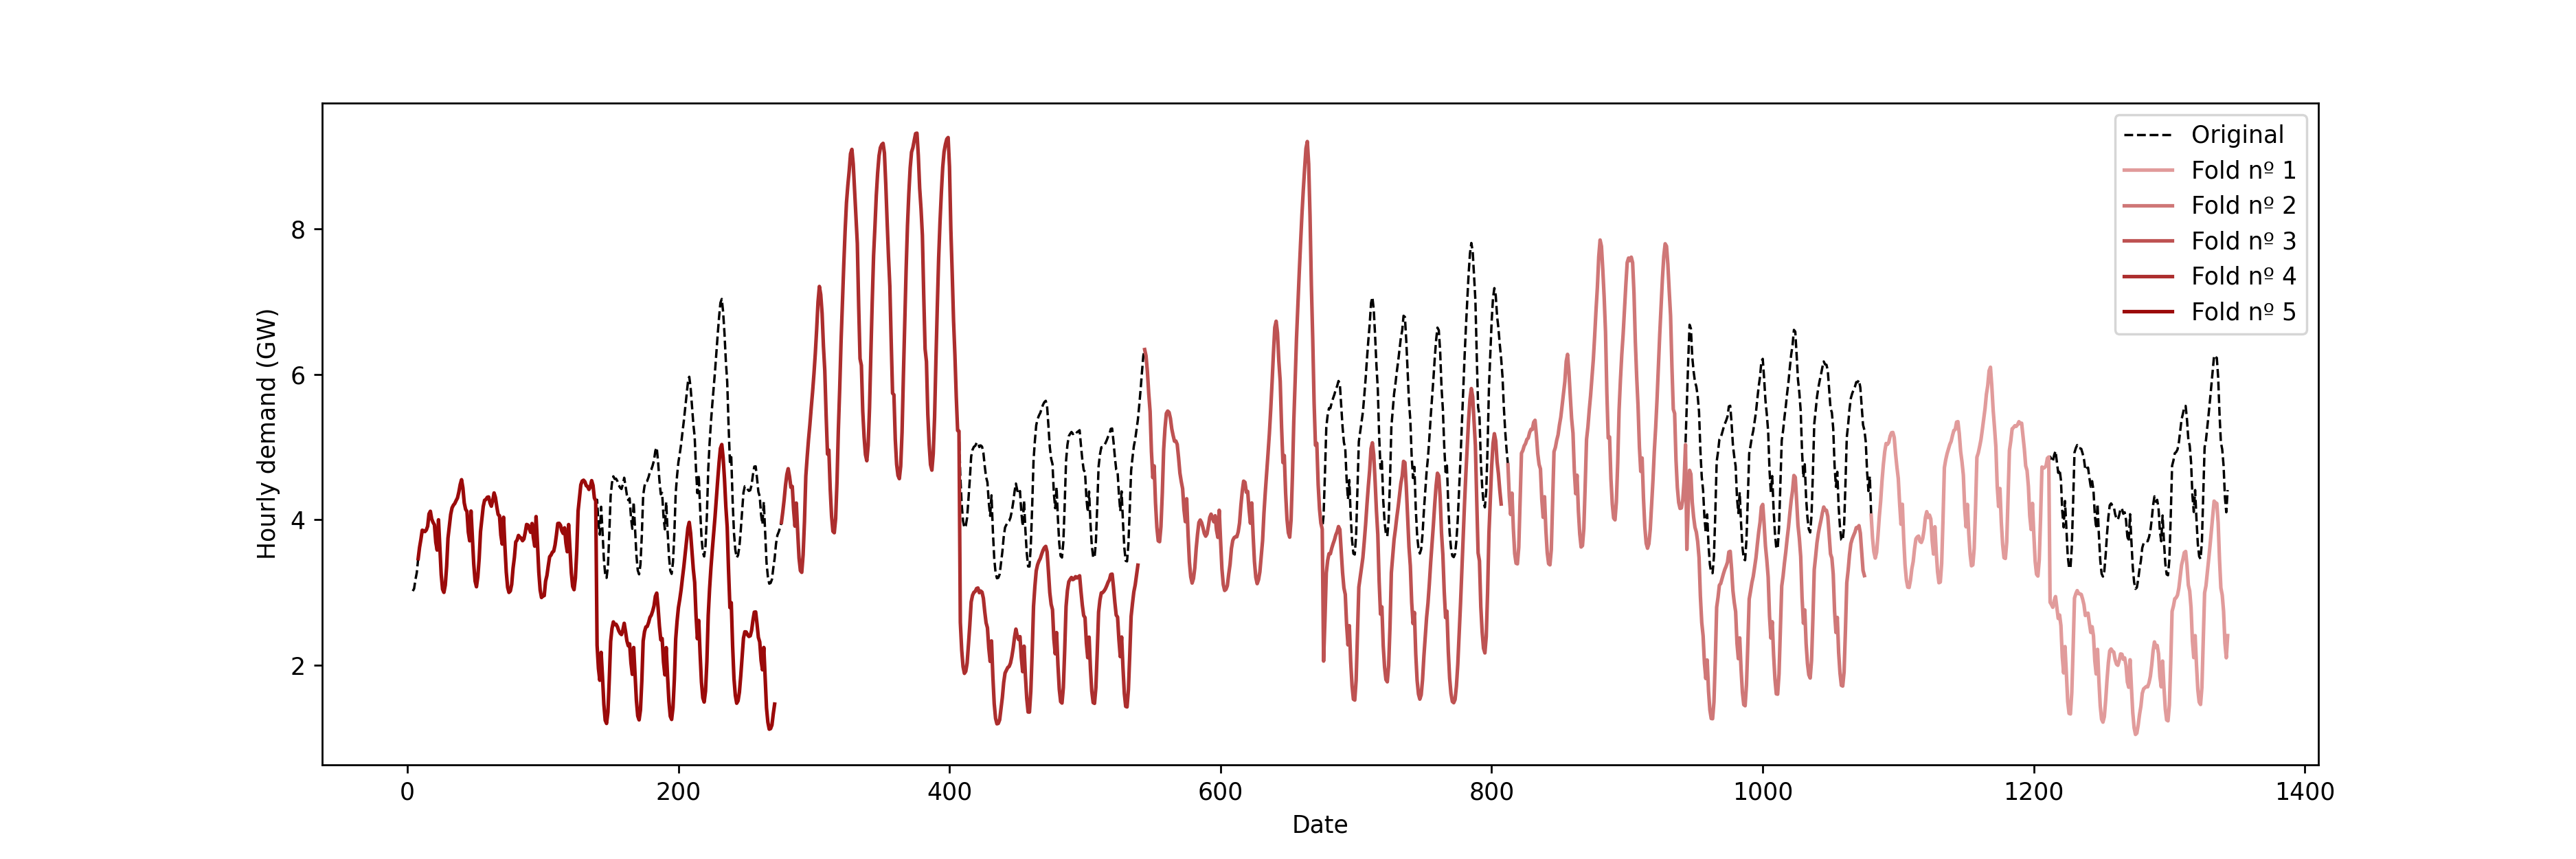
\includegraphics[width=1\textwidth]{Figures/timeseries/with-change-point/ts-with-change-point-5-folds.png}
    \caption{5-fold splits from the original dataset and with a change point in the test split.}
    \label{fig:app-timeseries-5-folds-cpoint}
\end{figure}

\begin{figure}[ht]
    \centering
    \begin{subfigure}[b]{\textwidth}
        \centering
        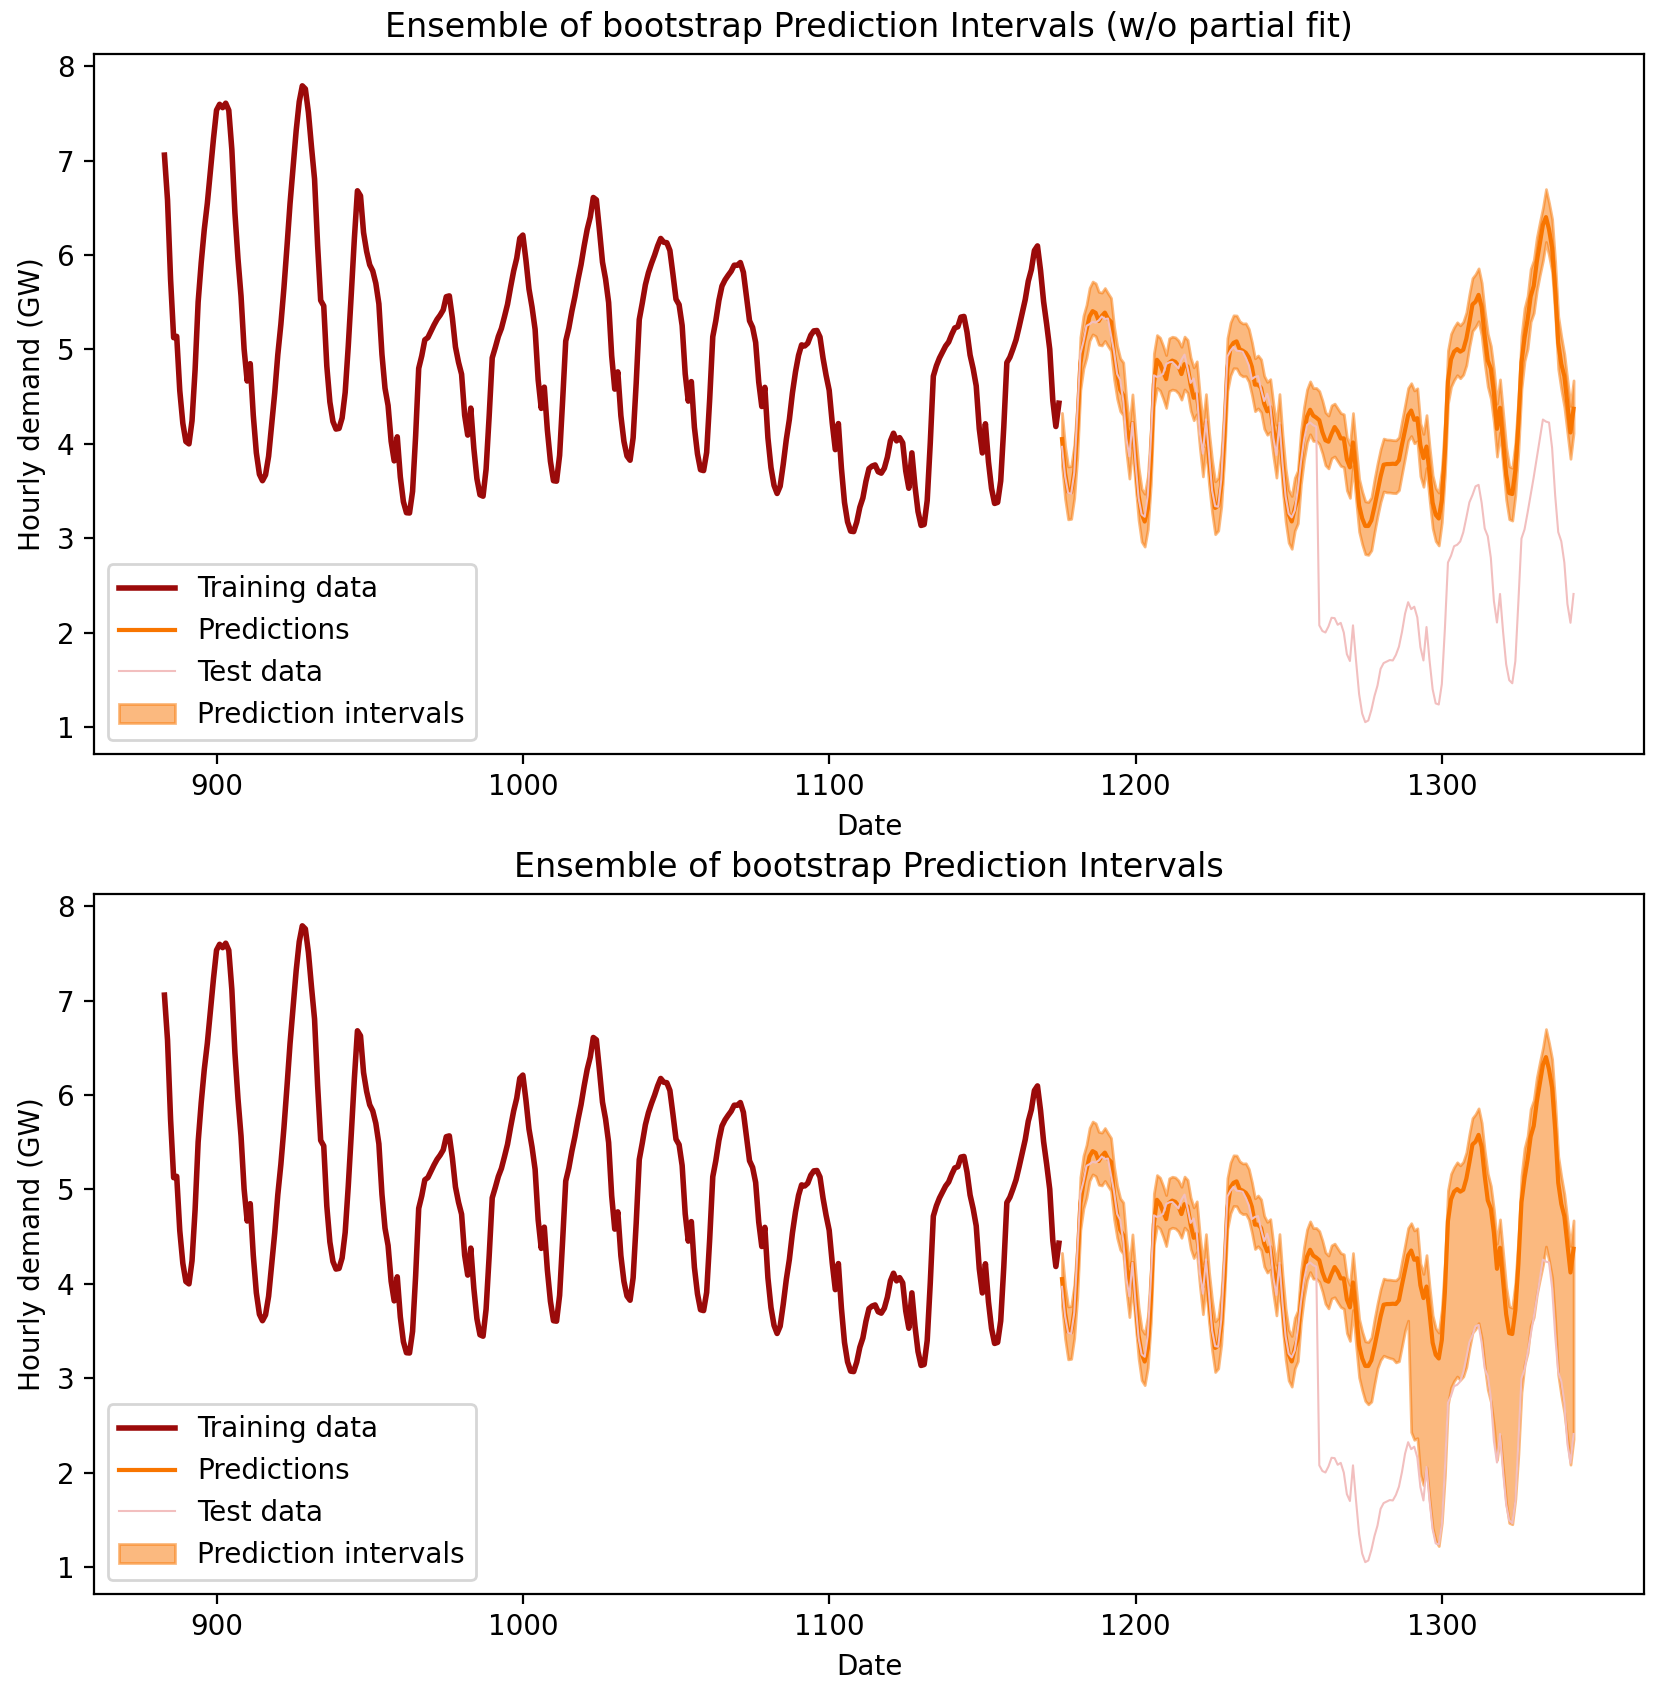
\includegraphics[width=.8\textwidth]{Figures/timeseries/with-change-point/prediction-intervals-timeseries-problem-with-change-point.png}
        \caption{Prediction intervals}
        \label{subfig:app-timeseries-prediction-intervals-cpoint}
    \end{subfigure}
    \hfill % adds horizontal space between figures
    \begin{subfigure}[b]{\textwidth} % Adjust the width to fit your needs
        \centering
        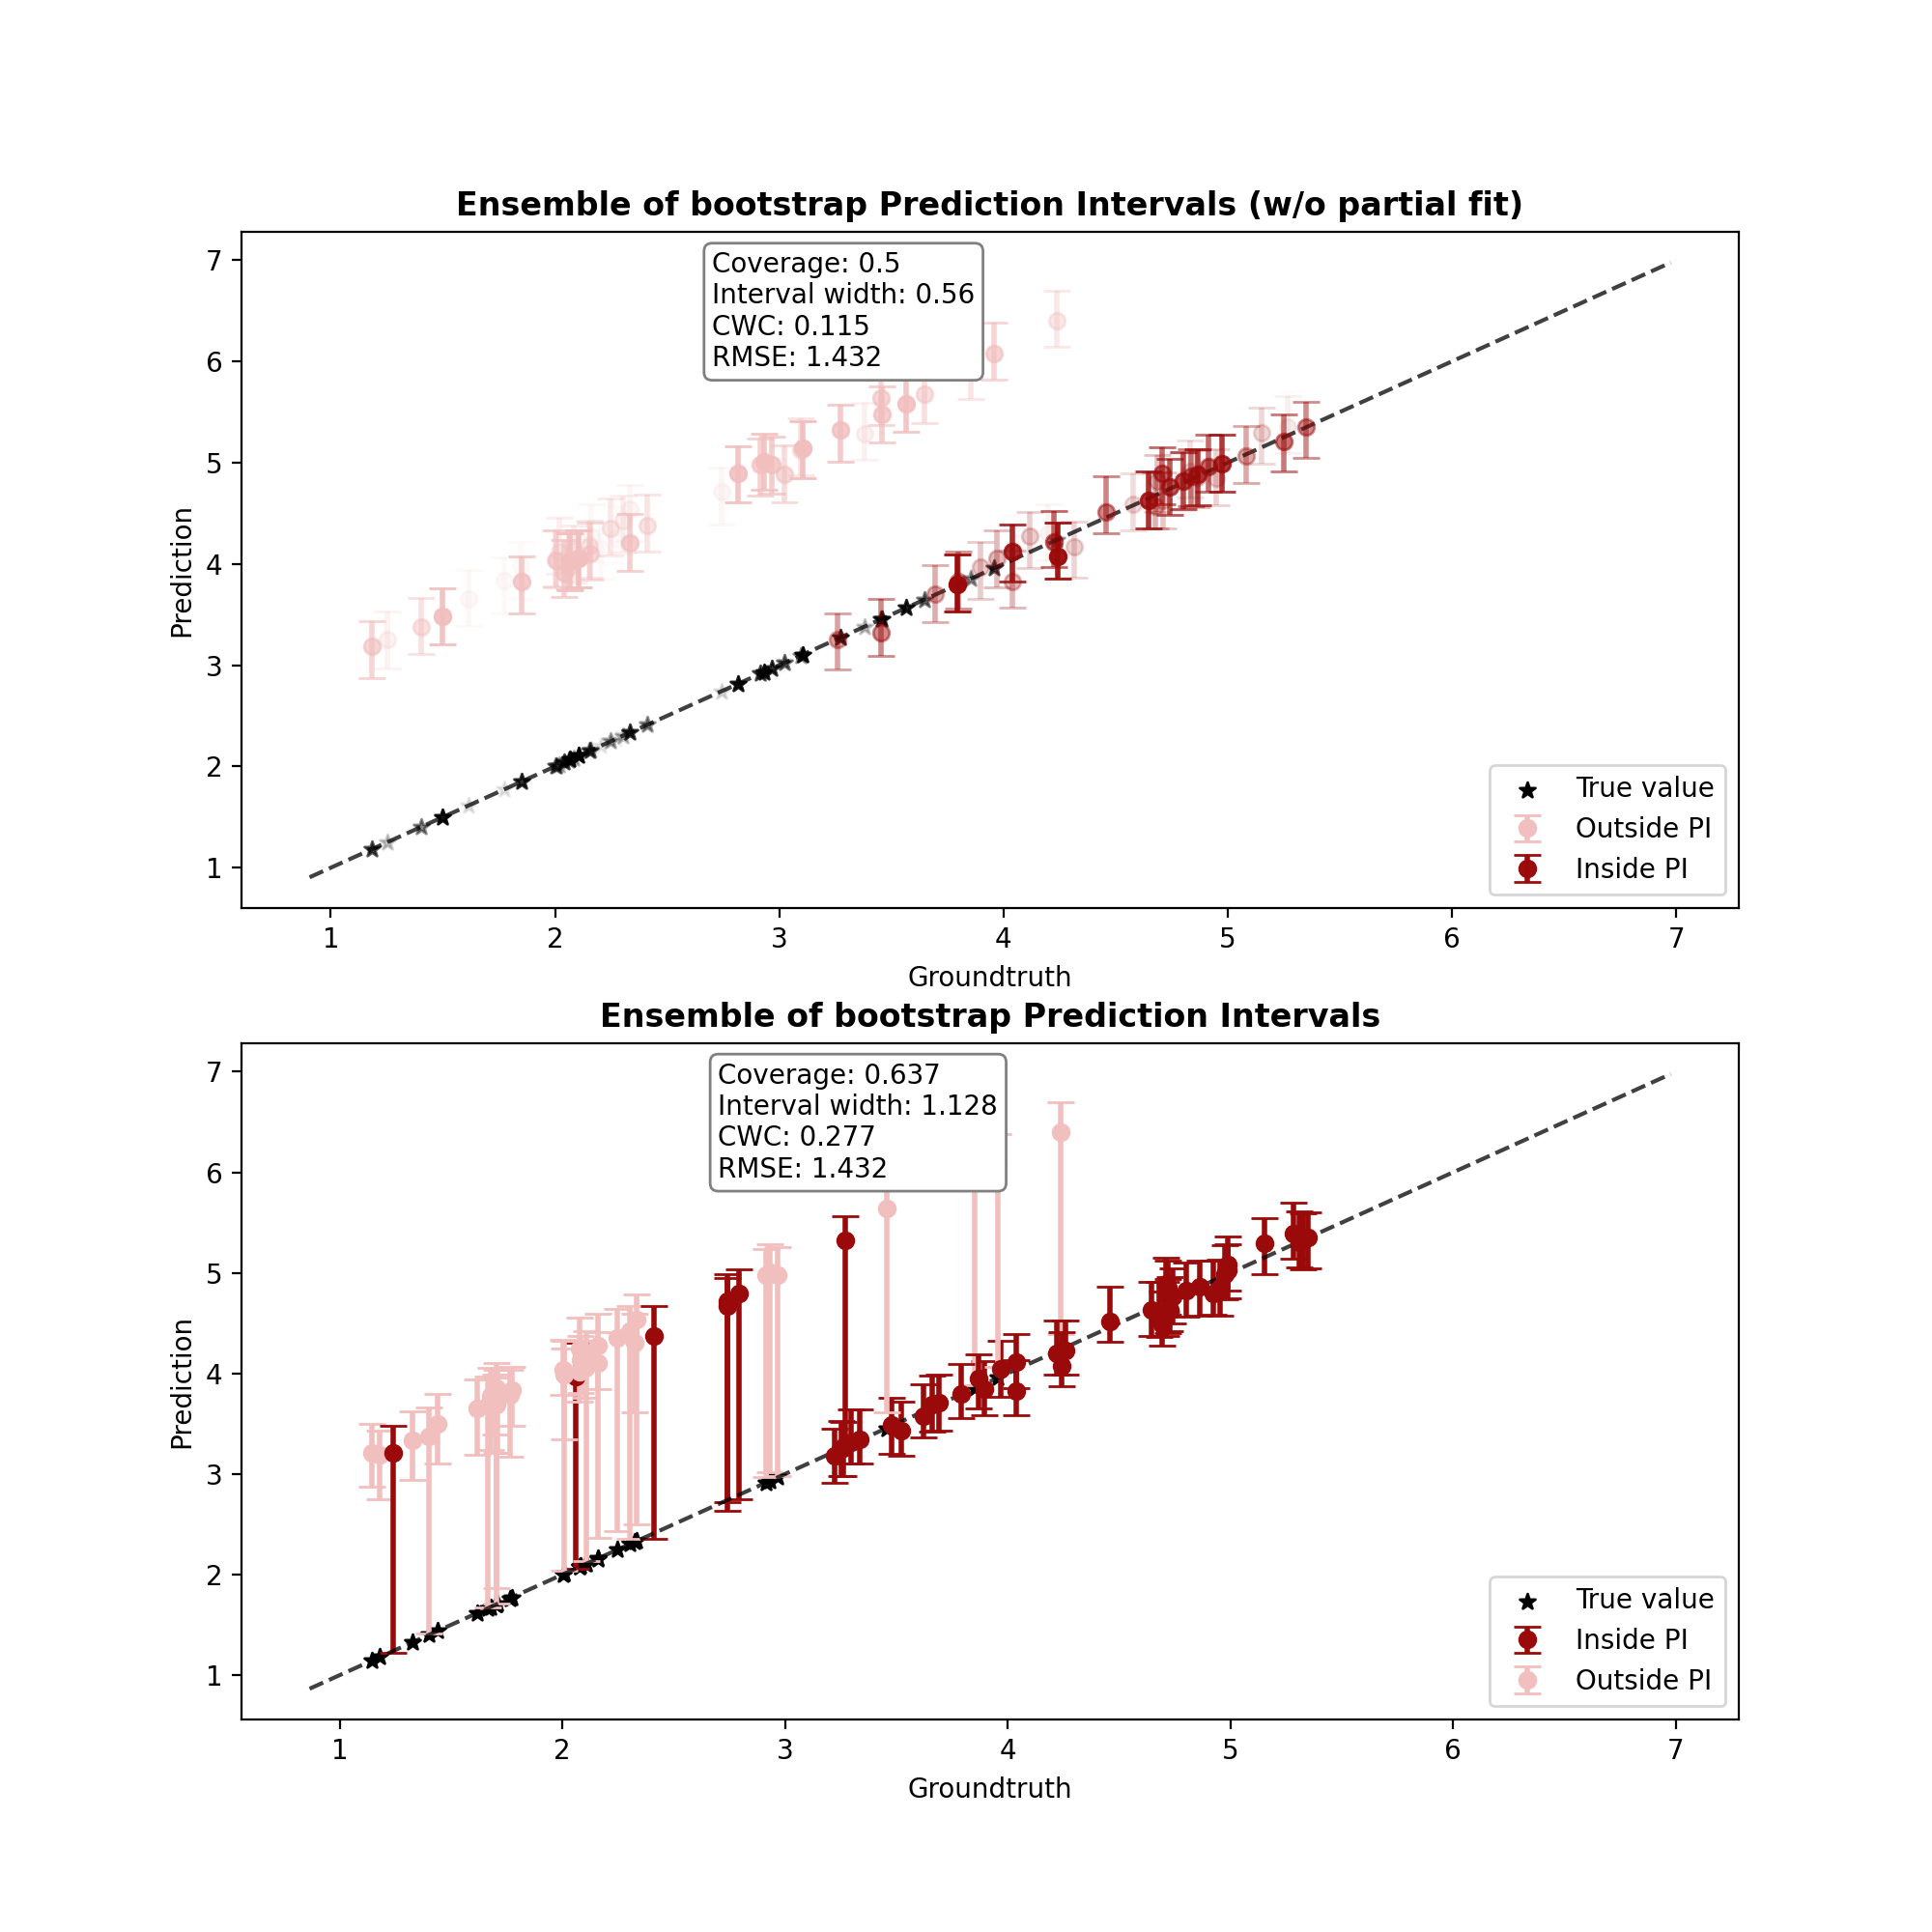
\includegraphics[width=.8\textwidth]{Figures/timeseries/with-change-point/average-goodness-timeseries-problem-with-change-point.png} % Adjust the filename and path
        \caption{Goodness of the prediction intervals (prediction vs. ground truth). Just a $50\%$ of the data is shown due to visualization reasons.}
        \label{subfig:app-timeseries-intervals-goodness-cpoint}
    \end{subfigure}
    \caption{Visualizations related to the prediction intervals for the test data (with a change point) \& the EnbPI strategy (without partial fit, top; and with it, bottom).}
    \label{fig:app-timeseries-intervals-cpoint}
\end{figure}

\begin{figure}[ht]
    \centering
    %\hspace{-10mm}
    \begin{subfigure}[b]{0.32\textwidth}
        \centering
        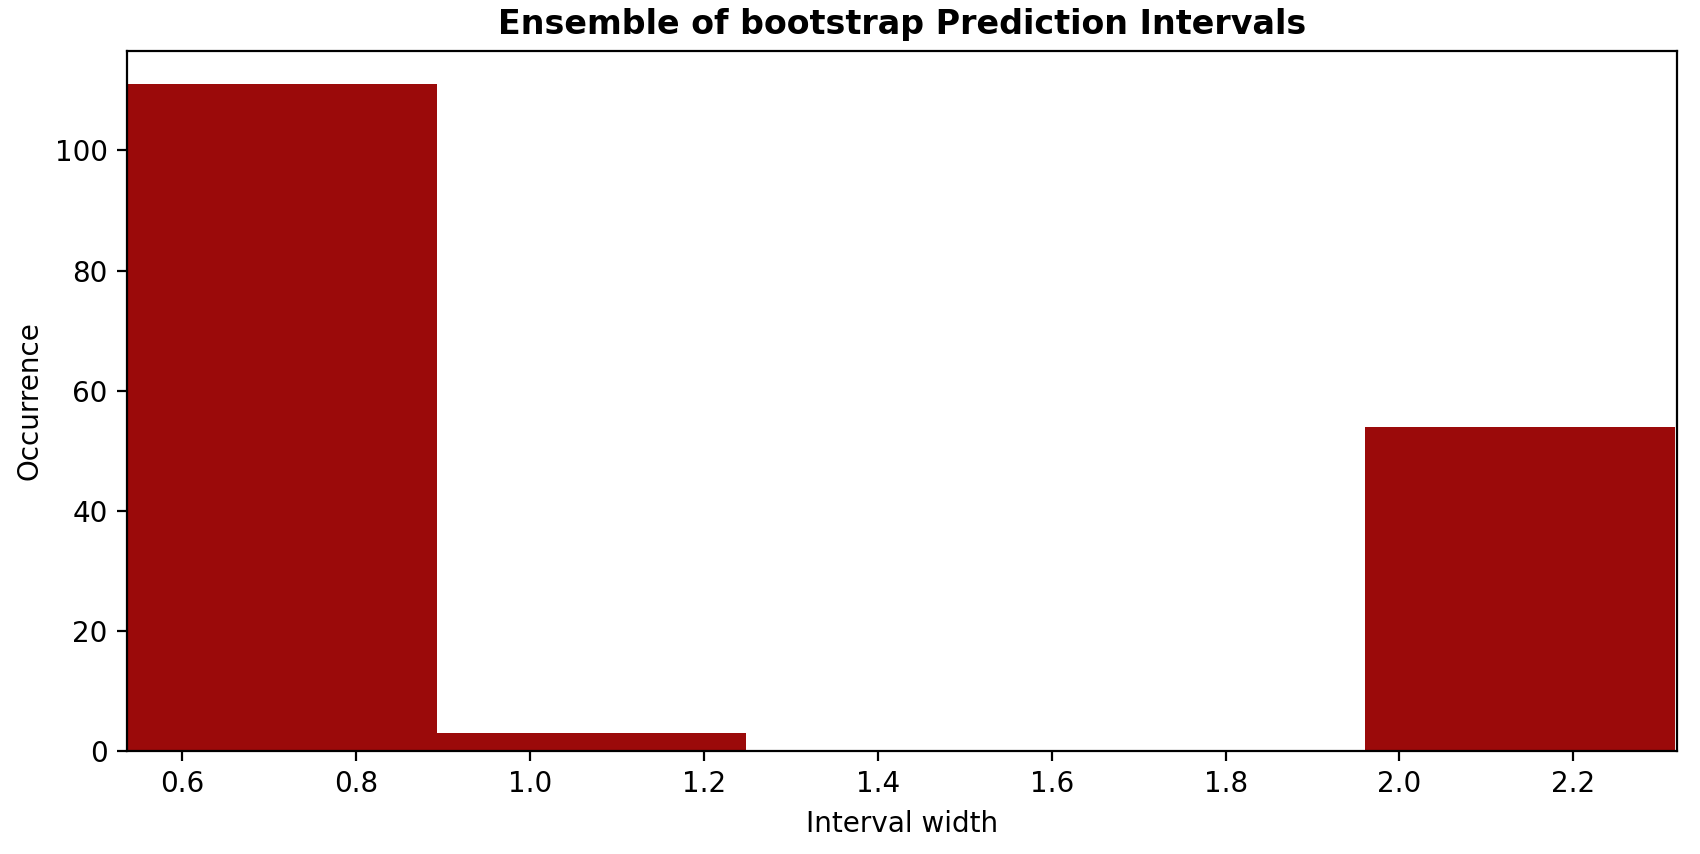
\includegraphics[width=1.15\textwidth, height=1.75\textwidth]{Figures/timeseries/with-change-point/width-occurrence-timeseries-problem-with-change-point.png}
        \caption{Intervals' width histograms}
        \label{subfig:app-timeseries-width-histograms-cpoint}
    \end{subfigure}
    \hfill
    \begin{subfigure}[b]{0.32\textwidth}
        \centering
        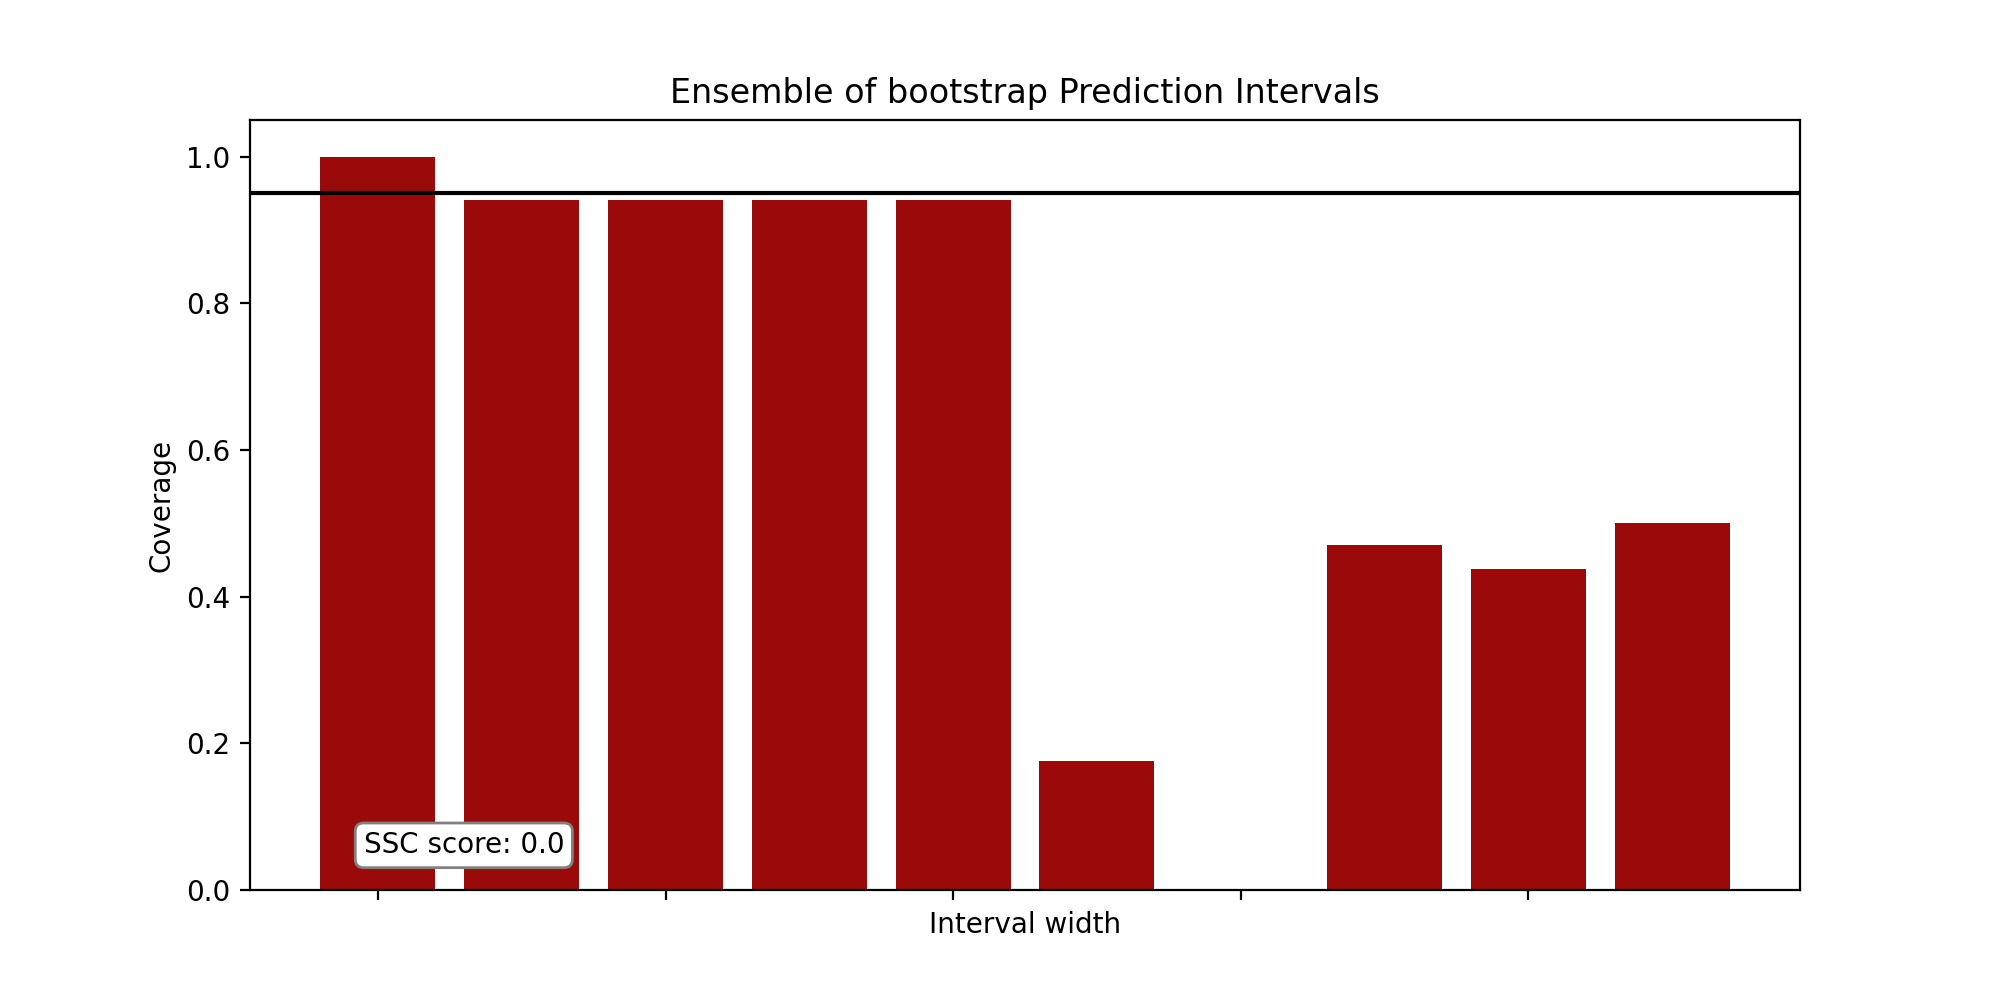
\includegraphics[width=1.15\textwidth, height=0.85\textwidth]{Figures/timeseries/with-change-point/coverage-vs-width-timeseries-problem-with-change-point.png}
        \caption{Coverage in function of intervals' width}
        \label{subfig:app-timeseries-coverage-width-cpoint}
    \end{subfigure}
    \hfill % adds horizontal space between figures
    \begin{subfigure}[b]{0.32\textwidth} % Adjust the width to fit your needs
        \centering
        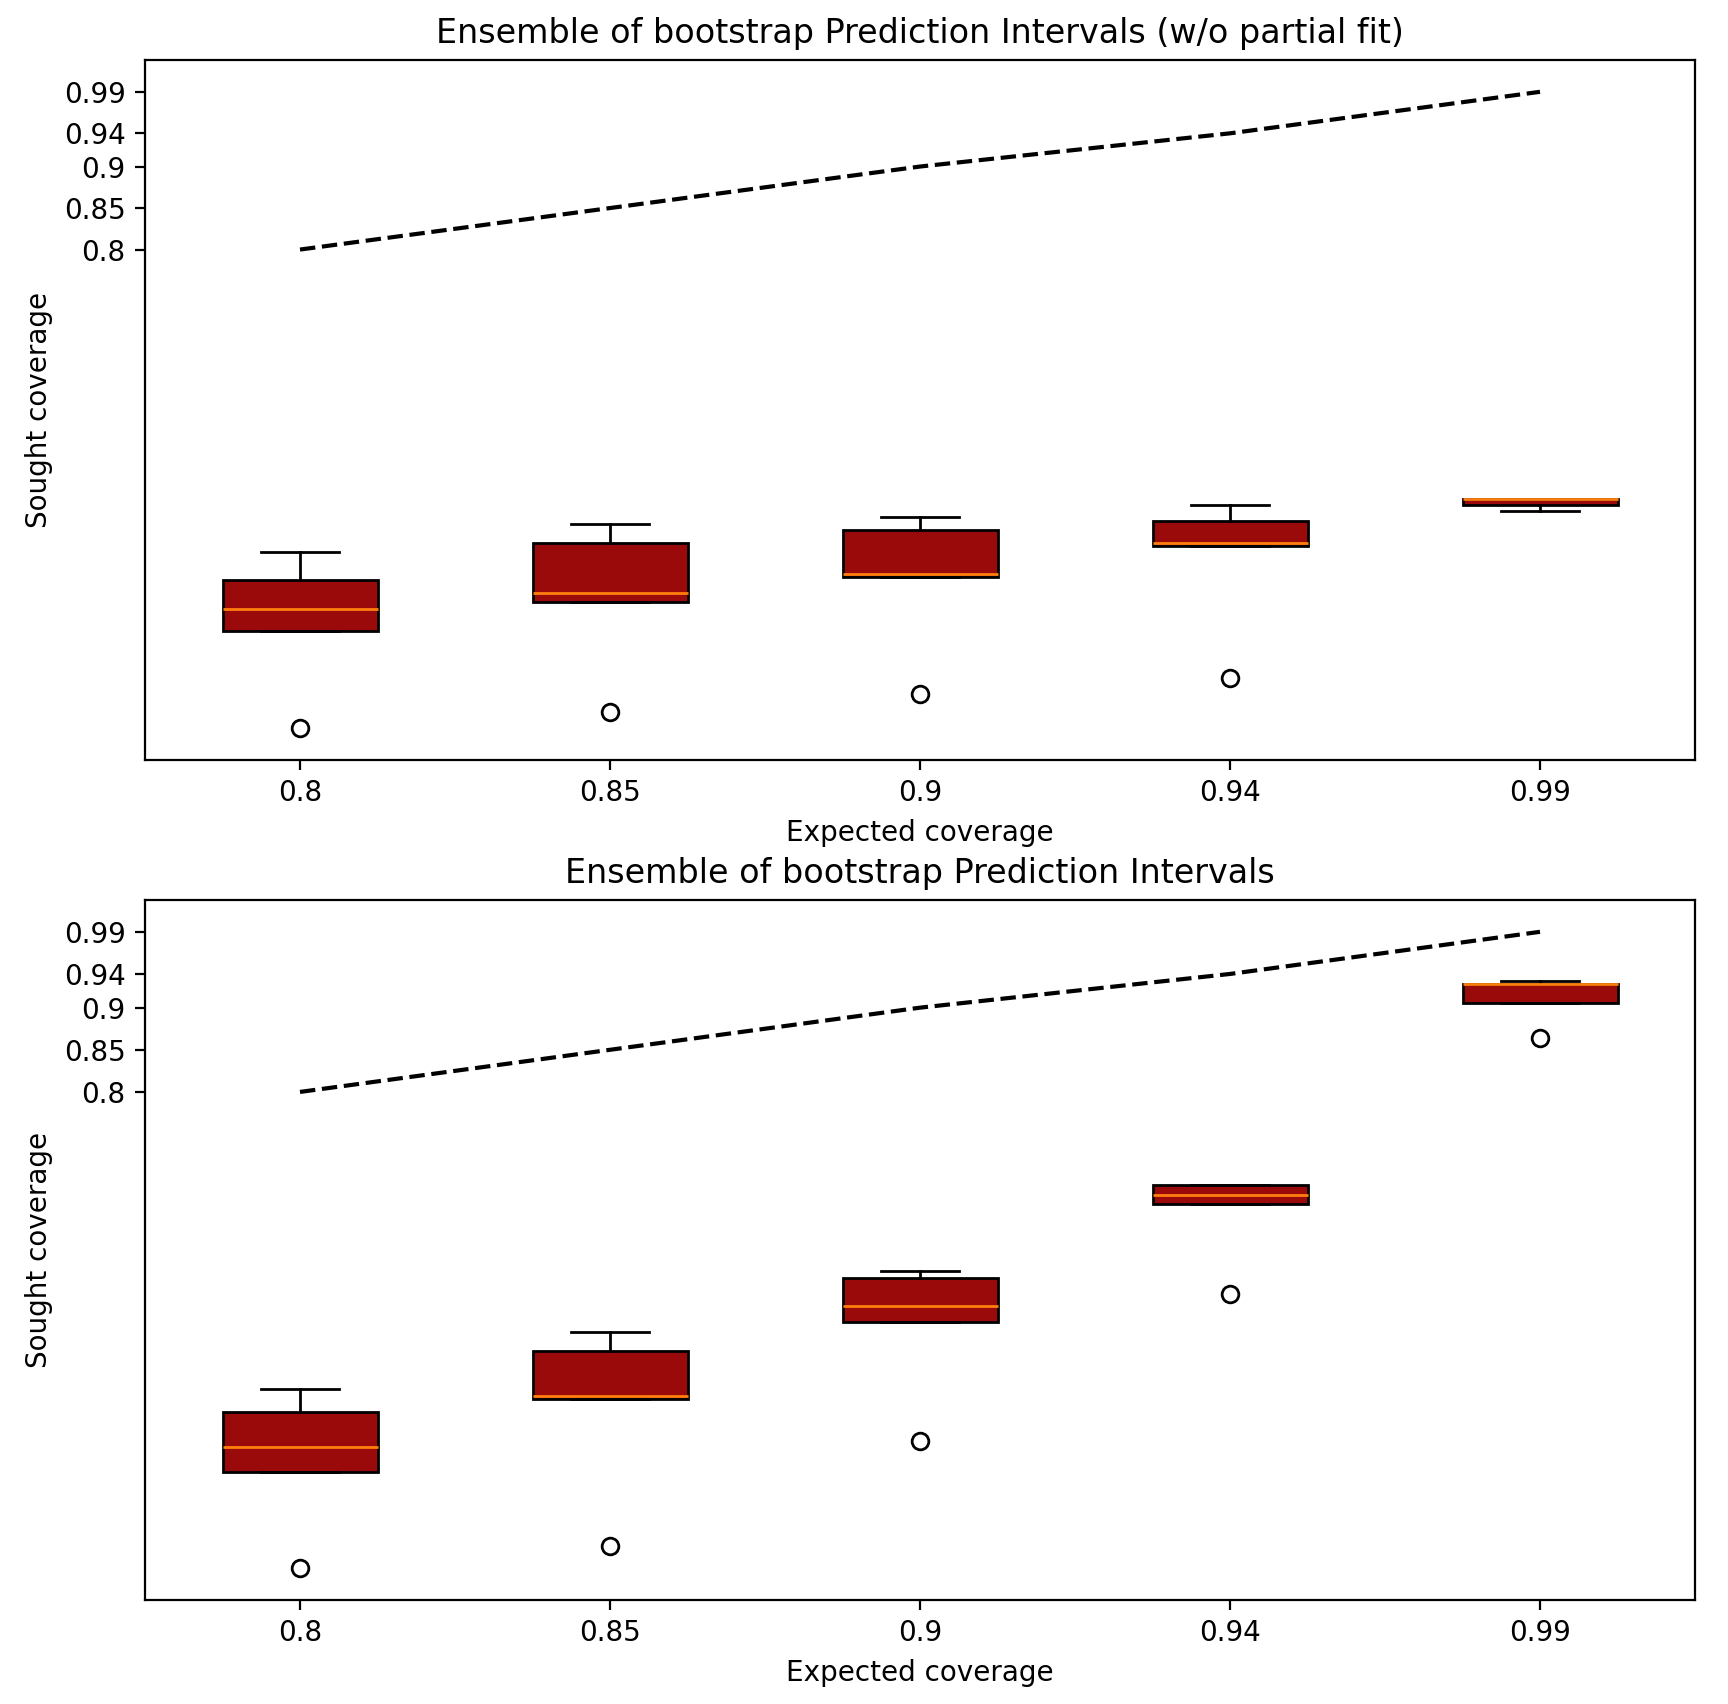
\includegraphics[width=1.15\textwidth, height=1.75\textwidth]{Figures/timeseries/with-change-point/coverage-vs-alpha-timeseries-problem-with-change-problem.png} % Adjust the filename and path
        \caption{Coverage in function of $\a$}
        \label{subfig:app-timeseries-coverage-alpha-cpoint}
    \end{subfigure}
    \caption{Visualizations related to width \& coverage distributions for the test data (with a change point) \& the EnbPI strategy (without partial fit, top; and with it, bottom).}
    \label{fig:app-timeseries-width-coverage-cpoint}
\end{figure}

\begin{figure}[ht]
    \centering
    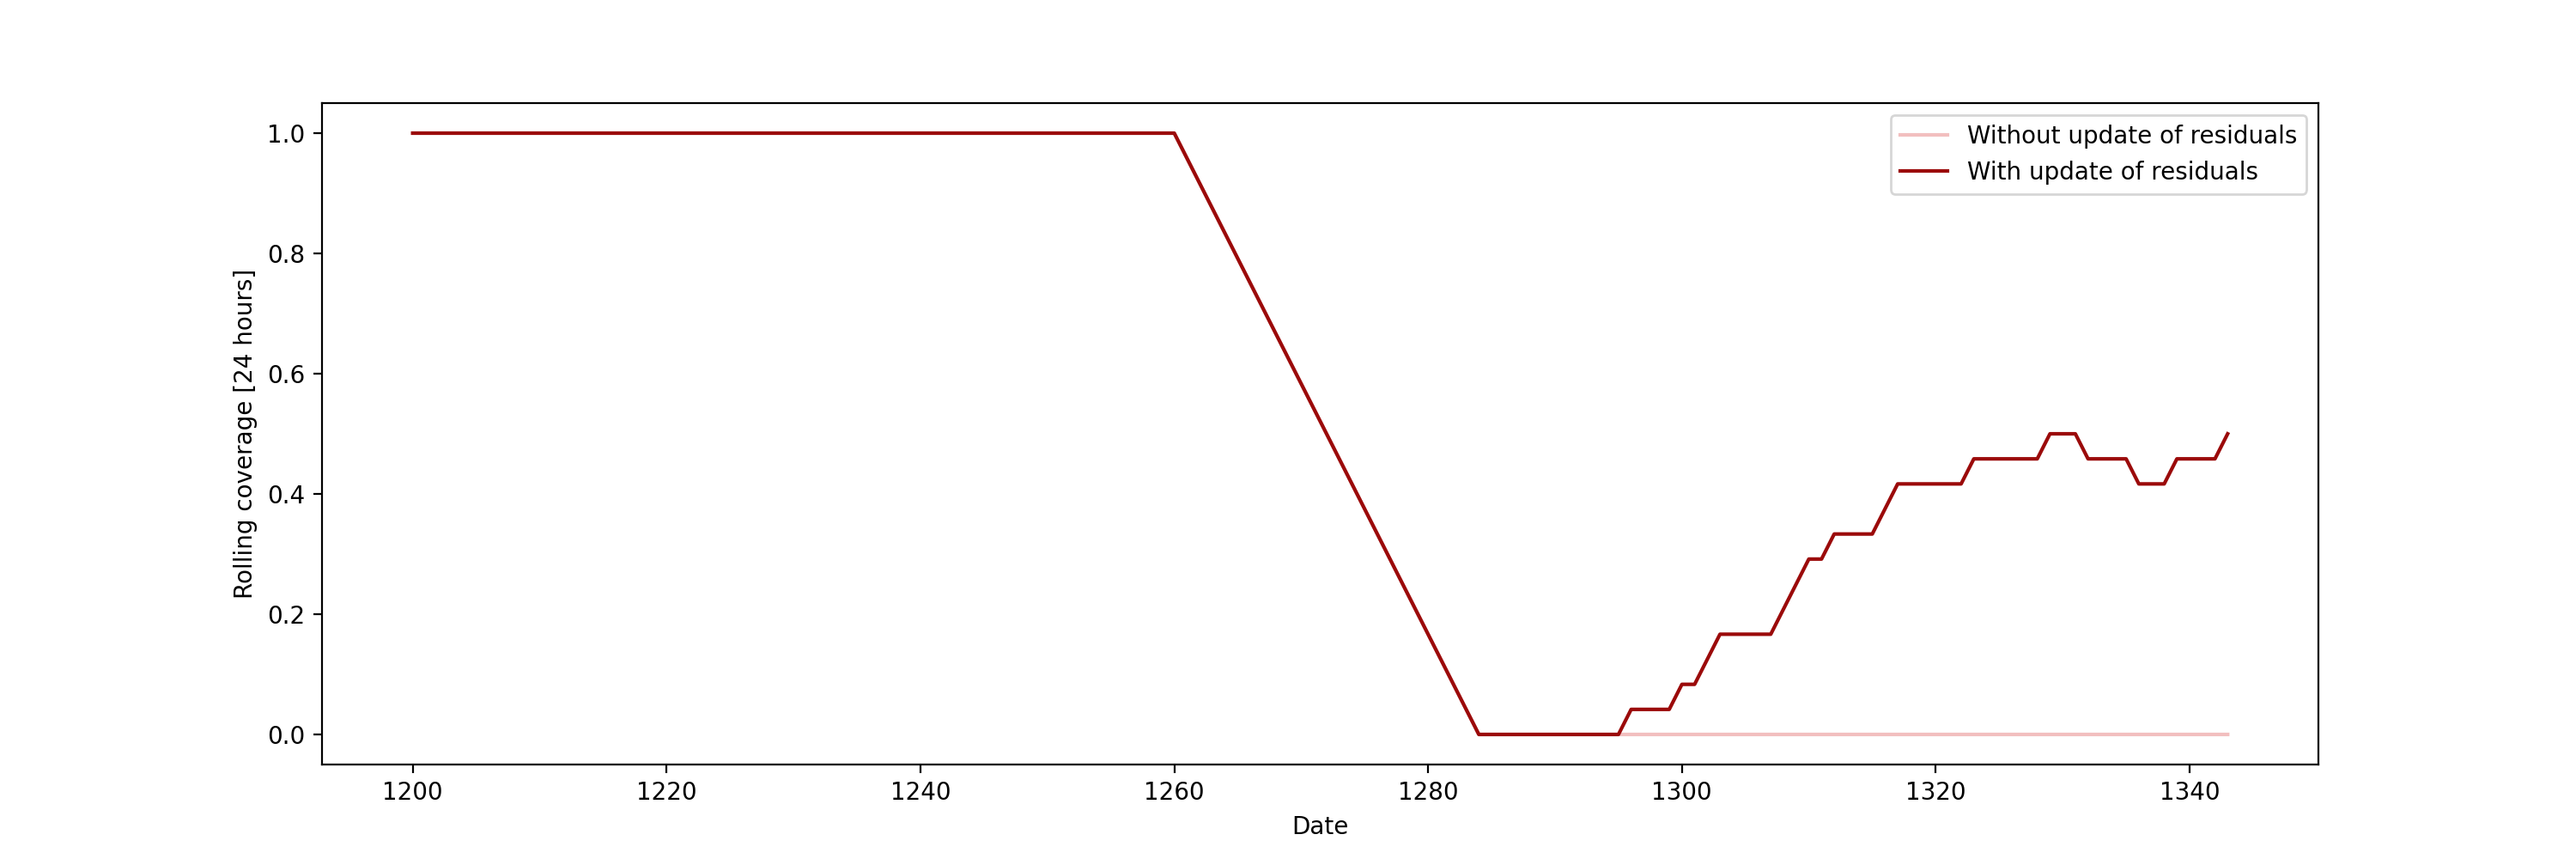
\includegraphics[width=\textwidth]{Figures/timeseries/with-change-point/rolling-coverage-with-change-point.png}
    \caption{Test data coverage (change point's dataset), for the EnbPI strategies, in function of time (grouped within 24h rolling windows).}
    \label{fig:app-timeseries-rolling-coverage-cpoint}
\end{figure}

\begin{figure}[ht]
    \centering
    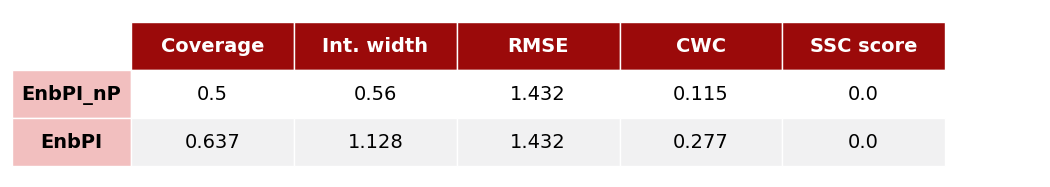
\includegraphics[width=\textwidth]{Figures/timeseries/with-change-point/metrics-table-timeseries-problem-with-change-point.png}
    \caption{Test data metrics for the EnbPI strategy and 1 particular experiment (no 5-folds CV) for $\a=0.05$ and the chage point dataset. From top to bottom: EnbPI without partial fit (EnbPI\_{}nP), EnbPI with it (EnbPI).}
    \label{fig:app-timeseries-metrics-cpoint}
\end{figure}

\begin{figure}[ht]
    \centering
    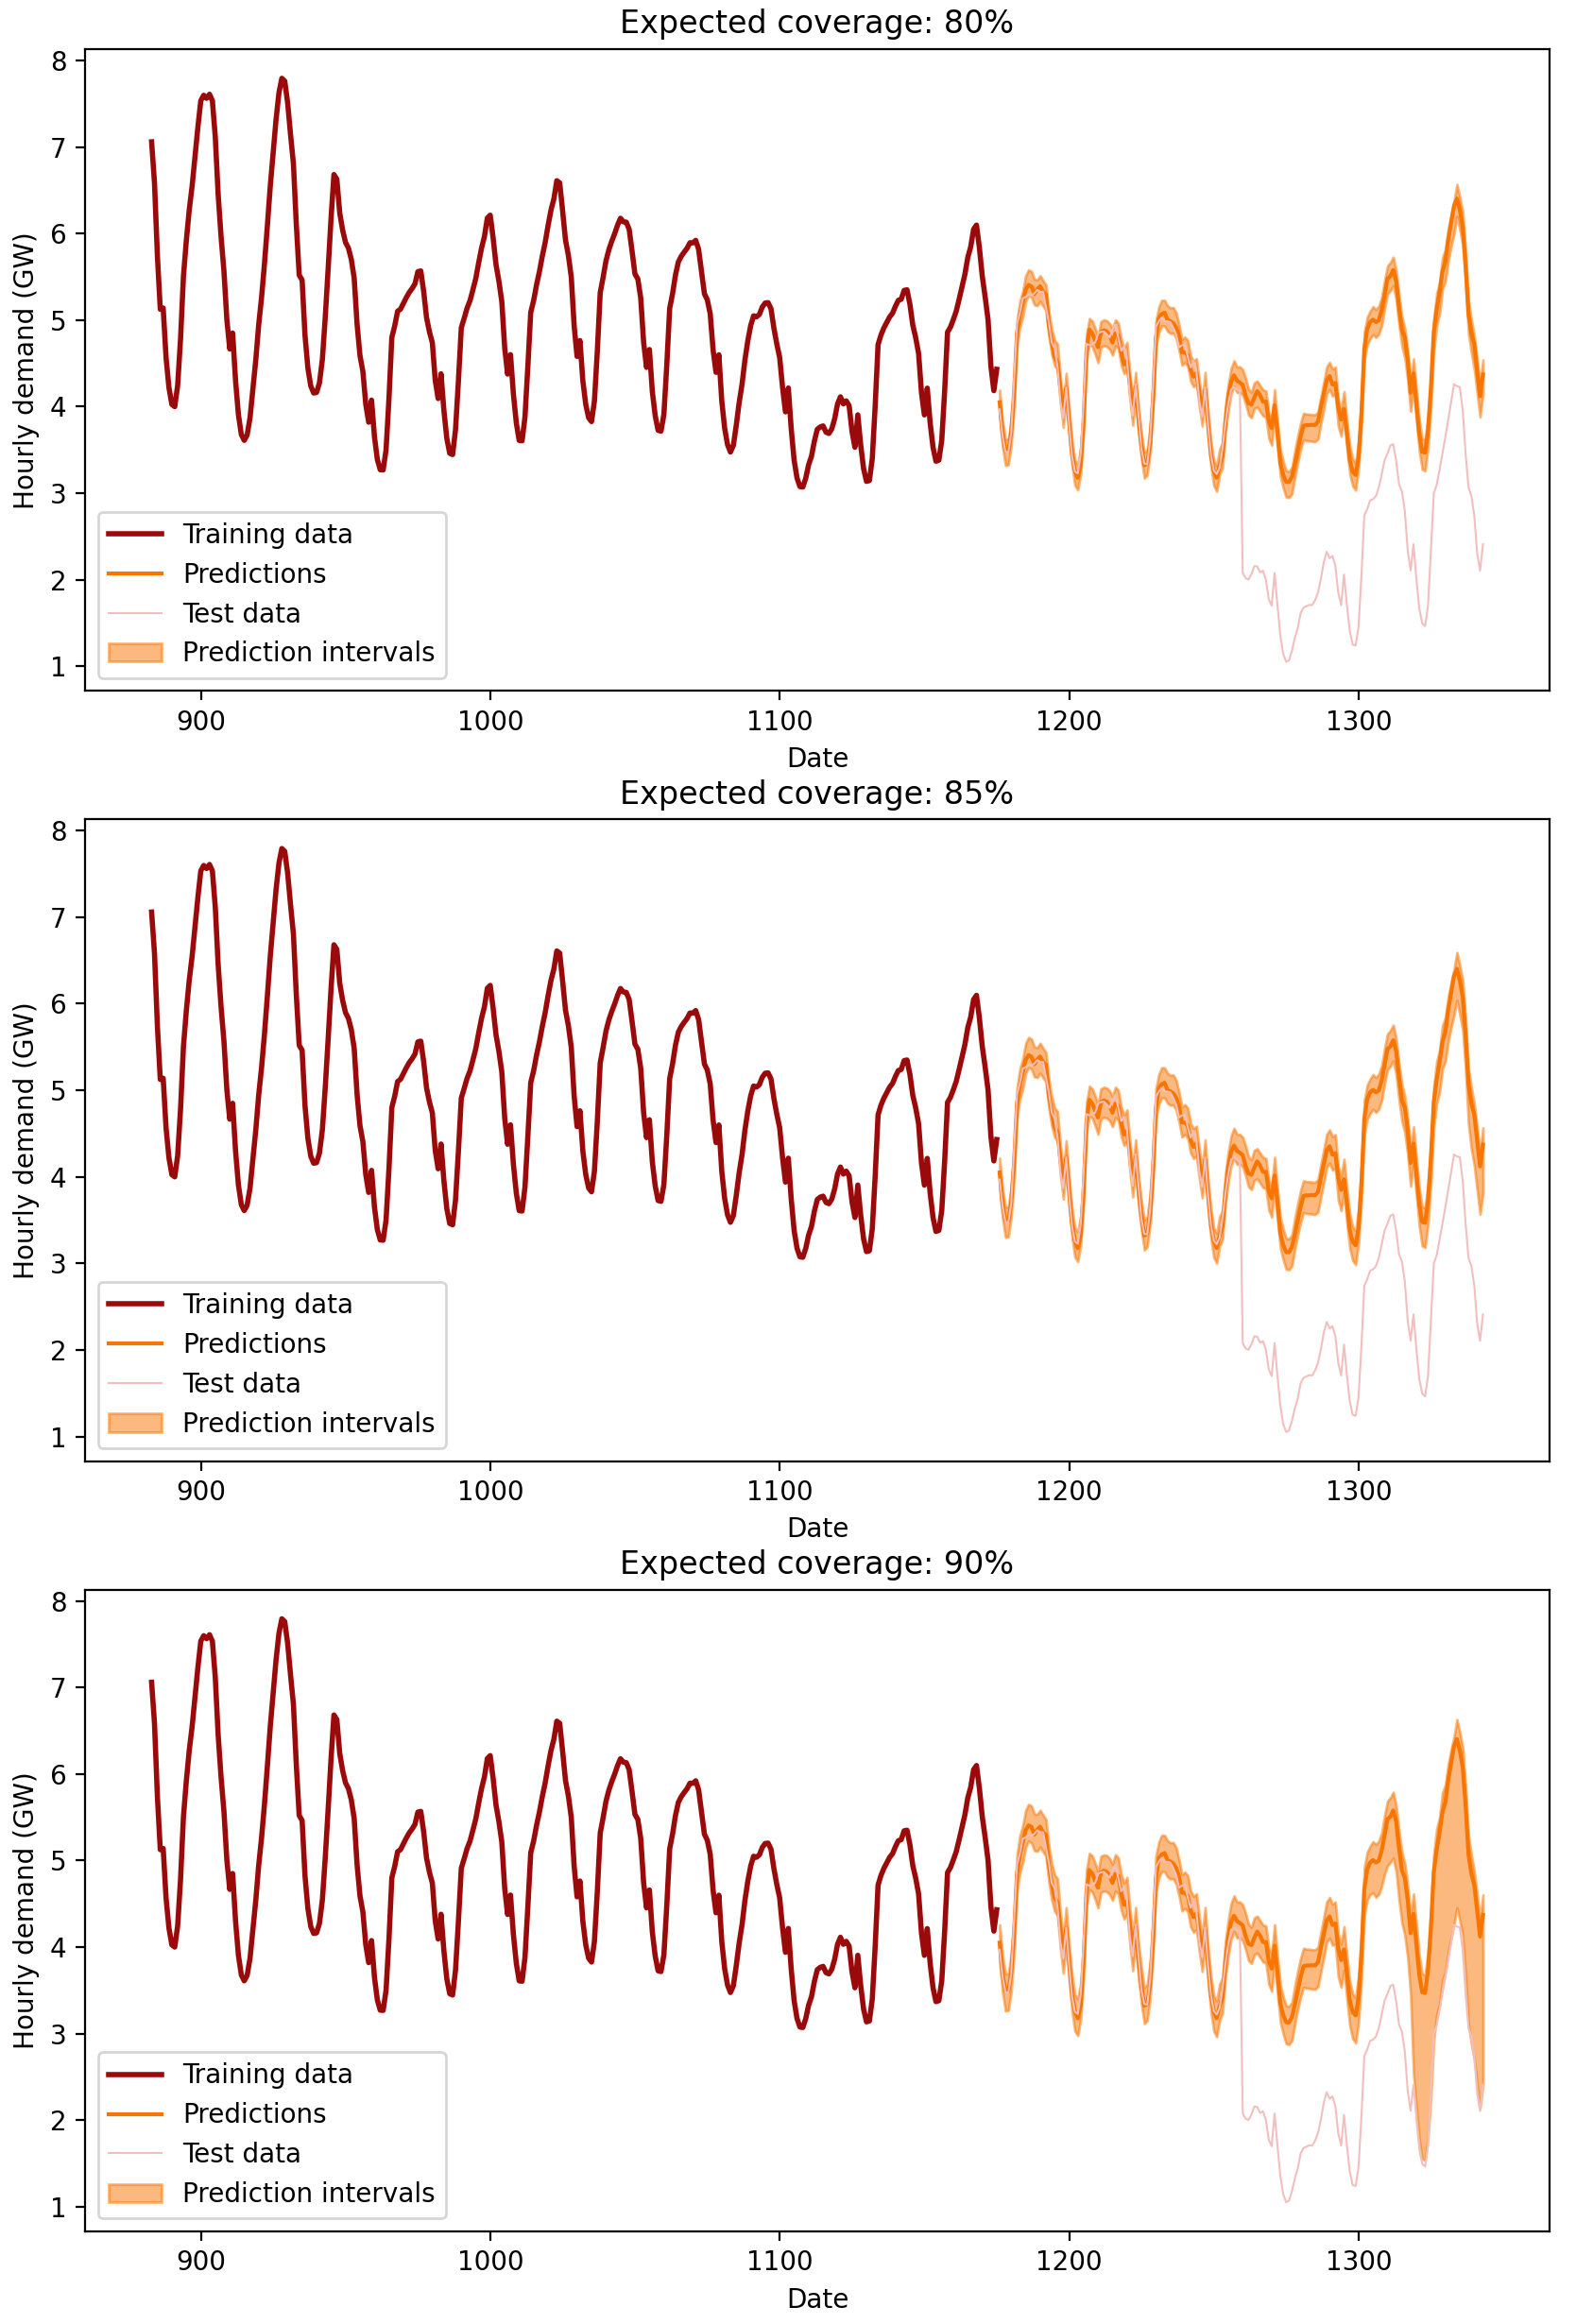
\includegraphics[width=\textwidth]{Figures/timeseries/with-change-point/prediction-intervals-in-function-of-miscoverage.png}
    \caption{Prediction intervals (change point's dataset) in function of time and for different values of $\a$.}
    \label{fig:app-timeseries-intervals-alpha-cpoint}
\end{figure}

%----------------------------------------------------------------------------------------
%	BIBLIOGRAPHY
%----------------------------------------------------------------------------------------

\printbibliography[heading=bibintoc]

%----------------------------------------------------------------------------------------

\end{document}  
